
\documentclass[reqno,11pt]{book}

%%%%%%%%%%%%%%%Setting for fast compiling
%\special{dvipdfmx:config z 0}
%\includeonly{chapters/contents}
%\includeonly{chapters/introduction}
%\includeonly{chapters/affinepaving}
%\includeonly{chapters/chapter5}

%packages
%\usepackage{color,graphicx}
%\usepackage{mathrsfs,amsbsy}
\usepackage{amssymb}
\usepackage{amsmath}
\usepackage{amsfonts}
\usepackage{bm}
\usepackage{caption,subcaption}
\usepackage{graphicx}
\usepackage{amsthm}
\usepackage{enumerate}
\usepackage{extarrows}
\usepackage[mathscr]{eucal}
\usepackage{float}
\usepackage{mathrsfs}
\usepackage{multicol}
\usepackage{multirow}
\usepackage[all,pdf]{xy}
\usepackage[a4paper,left=3cm,right=3cm,bottom=3cm]{geometry}
\usepackage[table,xcdraw]{xcolor} % before tikz-cd
\usepackage{tikz-cd}
\usepackage[colorlinks]{hyperref}
\usepackage{scalerel}
\usepackage{stackengine,wasysym}
\usepackage[width=0.5,tiewidth=0.7]{strands}
\usepackage{quiver}
\usepackage[shortlabels]{enumitem} %https://tex.stackexchange.com/questions/58852/possible-incompatibility-with-enumitem
\usepackage{array}
\usepackage{diagbox}
\usepackage{makecell}
\usepackage{adjustbox}
\usepackage{indentfirst}
\usepackage{pifont}
\usepackage{MA_Titlepage}

%\usepackage{nicematrix}%https://ctan.org/pkg/nicematrix?lang=en
%\usepackage[notcite,notref]{showkeys}

% showkeys  make label explicit on the paper
\hypersetup{
colorlinks=true,
citecolor=blue,
linkcolor=blue,
urlcolor=blue,
}

\numberwithin{equation}{section}

\theoremstyle{plain}
\newtheorem{theorem}{Theorem}[section]
\newtheorem{lemma}[theorem]{Lemma}
\newtheorem{proposition}[theorem]{Proposition}
\newtheorem{corollary}[theorem]{Corollary}
\newtheorem{claim}[theorem]{Claim}
\newtheorem{defn}[theorem]{Definition}
\newtheorem{ques}[theorem]{Question}
\newtheorem*{bbox}{Black box}
\newtheorem{eg}[theorem]{Example}
\newtheorem{ex}[theorem]{Exercise}
\newtheorem{fact}[theorem]{Fact}
\newtheorem{warning}[theorem]{Warning}
\newtheorem{setting}[theorem]{Setting}
\newtheorem{conj}[theorem]{Conjecture}
\newtheorem*{notation}{Conventions and Notations}


\theoremstyle{plain}
\newtheorem{thmsub}{Theorem}[subsection]
\newtheorem{lemmasub}[thmsub]{Lemma}
\newtheorem{corollarysub}[thmsub]{Corollary}
\newtheorem{propositionsub}[thmsub]{Proposition}
\newtheorem{defnsub}[thmsub]{Definition}

\numberwithin{equation}{section}


\theoremstyle{remark}

\newtheorem{remark}[theorem]{Remark}
\newtheorem{remarks}{Remarks}


\newtheoremstyle{theoremletter}{4mm}{1mm}{\itshape}{ }{\bfseries}{}{ }{}
\theoremstyle{theoremletter}
\newtheorem{theoremA}{Theorem}
\renewcommand{\thetheoremA}{A}
\newtheorem{theoremB}{Theorem}
\renewcommand{\thetheoremB}{B}

%\renewcommand\thefootnote{\fnsymbol{footnote}}
%dont use number as footnote symbol, use this command to change

\DeclareMathOperator{\EGG}{\operatorname{E}\!}
\DeclareMathOperator{\BGG}{\operatorname{B}\!}
\DeclareMathOperator{\GL}{\operatorname{GL}}
\DeclareMathOperator{\SL}{\operatorname{SL}}
\DeclareMathOperator{\supp}{supp}
\DeclareMathOperator{\dist}{dist}
\DeclareMathOperator{\vol}{vol}
\DeclareMathOperator{\diag}{diag}
\DeclareMathOperator{\tr}{tr}
\DeclareMathOperator{\Img}{\operatorname{Im}}
\DeclareMathOperator{\gr}{\operatorname{gr}}
\DeclareMathOperator{\Id}{\operatorname{Id}}
\DeclareMathOperator{\rep}{\operatorname{rep}}
\DeclareMathOperator{\Rep}{\operatorname{Rep}}
\DeclareMathOperator{\Irr}{\operatorname{Irr}}
\DeclareMathOperator{\RRep}{\widetilde{\operatorname{Rep}}}
\DeclareMathOperator{\Mod}{\operatorname{Mod}}
\DeclareMathOperator{\catmod}{\operatorname{mod}}
\DeclareMathOperator{\Ind}{\operatorname{Ind}}
\DeclareMathOperator{\Res}{\operatorname{Res}}
\DeclareMathOperator{\Coh}{\operatorname{Coh}}
\DeclareMathOperator{\Tor}{\operatorname{Tor}}
\newcommand{\Dcoh}{\mathcal{D}_{\operatorname{Coh}}}%%%This one shows the difference between \DeclareMathOperator and \newcommand
\DeclareMathOperator{\Hom}{\operatorname{Hom}}
\DeclareMathOperator{\Ext}{\operatorname{Ext}}
\DeclareMathOperator{\gldim}{\operatorname{gl.dim}}
\DeclareMathOperator{\projdim}{\operatorname{proj.dim}}
\DeclareMathOperator{\injdim}{\operatorname{inj.dim}}
\DeclareMathOperator{\dimv}{\operatorname{\underline{\mathbf{dim}}}}
\DeclareMathOperator{\Alggp}{\text{-Alg gp}}
\DeclareMathOperator{\Pic}{\operatorname{Pic}}
\DeclareMathOperator{\Jac}{\operatorname{Jac}}
\DeclareMathOperator{\pt}{\operatorname{pt}}
\DeclareMathOperator{\ptt}{\operatorname{par}}
\DeclareMathOperator{\Frac}{\operatorname{Frac}}
\DeclareMathOperator{\Rpt}{\operatorname{R}}
\DeclareMathOperator{\Rptc}{\operatorname{\mathcal{R}}}
\DeclareMathOperator{\Spt}{\operatorname{S}}
\DeclareMathOperator{\Sptc}{\operatorname{\mathcal{S}}}
\DeclareMathOperator{\Kcurl}{\operatorname{\mathcal{K}}}
\DeclareMathOperator{\Hcurl}{\operatorname{\mathcal{H}}}
\DeclareMathOperator{\eu}{\operatorname{eu}}
\DeclareMathOperator{\Eu}{\operatorname{Eu}}
\newcommand{\Spec}{\operatorname{Spec}}
\DeclareMathOperator{\St}{\mathcal{Z}}

\DeclareMathOperator{\str}{\operatorname{str}}


\DeclareMathOperator{\Mor}{\operatorname{Mor}}
\DeclareMathOperator{\rad}{\operatorname{rad}}
\DeclareMathOperator{\ind}{\operatorname{ind}}
\DeclareMathOperator{\End}{\operatorname{End}}
\DeclareMathOperator{\Modup}{\overline{\operatorname{mod}}}
\DeclareMathOperator{\Moddown}{\underline{\operatorname{mod}}}
\DeclareMathOperator{\Homup}{\overline{\operatorname{Hom}}}
\DeclareMathOperator{\Homdown}{\underline{\operatorname{Hom}}}

\newcommand{\Gr}{\operatorname{Gr}}
\newcommand{\Grr}{\operatorname{Gr}}
\newcommand{\Gralg}[1]{\operatorname{Gr}^{#1}}
\newcommand{\Grq}{\operatorname{Gr}^{KQ}}
\newcommand{\Flag}[1]{\operatorname{Flag}_{#1}}
\newcommand{\Flagstr}[1]{\operatorname{Flag}_{#1,\operatorname{str}}}
\DeclareMathOperator{\Flagd}{\operatorname{Flag}_{d}}
\DeclareMathOperator{\Flagdstr}{\operatorname{Flag}_{d,\operatorname{str}}}
\newcommand{\dimvec}[1]{\mathbf{#1}}
\newcommand{\abdimvec}[1]{|\dimvec{#1}|}
\newcommand{\ftdimvec}[1]{\underline{\dimvec{#1}}}
\newcommand{\absgp}[1]{\mathbb{#1}}
\newcommand{\ww}{\varpi}
\newcommand{\Ri}{\operatorname{R}^i\!\!}
\newcommand{\AS}{\operatorname{AS}}
\newcommand{\chern}{\operatorname{ch}^{*}}
\newcommand{\Td}{\operatorname{Td}}
\DeclareMathOperator{\MinWd}{\operatorname{Min}(\absgp{W}_{\abdimvec{d}},W_{\dimvec{d}})}
\DeclareMathOperator{\Compd}{\operatorname{Comp}_{\dimvec{d}}}
\DeclareMathOperator{\Shuffled}{\operatorname{Shuffle}_{\dimvec{d}}}
\newcommand{\WWd}{\absgp{W}_{\abdimvec{d}}}
\newcommand{\Wd}{W_{\dimvec{d}}}
\newcommand{\norm}[1]{\Vert{#1}\Vert}
\newcommand{\ord}{\operatorname{ord}}
\newcommand{\orde}{\operatorname{ord}_e }
\newcommand{\shorttimes}{\!\times\!}
\newcommand{\oder}{\;\;\text{ or }\;\;}
\newcommand{\representation}[2]{\genfrac{}{}{0pt}{3}{\phantom{000}#2\phantom{00}}{#1}}
\newcommand{\Omcell}{\Omega}
\newcommand{\OOmcell}{\boldsymbol{\Omega}}
\newcommand{\Vcell}{\mathcal{V}}
\newcommand{\VVcell}{\boldsymbol{\mathcal{V}}}
\newcommand{\Ocell}{\mathcal{O}}
\newcommand{\OOcell}{\boldsymbol{\mathcal{O}}}
\newcommand{\preimage}[1]{\widetilde{#1}}
\newcommand{\fakestar}{*}
%https://tex.stackexchange.com/questions/96549/how-do-i-write-above-a-left-right-arrow
%\makeatletter
%\newcommand\xleftrightarrow[2][]{%
%  \ext@arrow 9999{\longleftrightarrowfill@}{#1}{#2}}
%\newcommand\longleftrightarrowfill@{%
%  \arrowfill@\leftarrow\relbar\rightarrow}
%\makeatother
\newcommand{\inCell}[2]
{\setlength{\fboxrule}{0pt} %%https://tex.stackexchange.com/questions/393676/remove-border-of-a-framebox
\fbox{
  \begin{minipage}{1cm}
    \centering
      {\hspace{-0.13cm}\textcolor{red}{$\scriptstyle {#1}$} \hfill $\,$}%
      \linebreak 
      {$#2$}%
      \linebreak 
      \vspace{0cm}
  \end{minipage}
  }
}
%global settings
\setlength\parindent{15pt}
\setlength\intextsep{0cm}
\setlength\textfloatsep{0cm}
\def\arraystretch{1.2}
\setcounter{secnumdepth}{3}
\allowdisplaybreaks


\makeatletter
\preto\env@matrix{\renewcommand{\arraystretch}{0.6}
\setlength\arraycolsep{1pt}}
\makeatother

% HIGHLIGHTING

%\newcommand{\lbox}{\adjustbox{cfbox=red, margin=-\fboxrule-\fboxsep}}
\newcommand{\lbox}{\adjustbox{}}
% from https://tex.stackexchange.com/questions/63545/big-tilde-in-math-mode

%https://tex.stackexchange.com/questions/456307/invalid-use-of-intertext-in-aligned
\newcommand{\alignedintertext}[1]{%
  \noalign{%
    \vskip\belowdisplayshortskip
    \vtop{\hsize=\linewidth#1\par
    \expandafter}%
    \expandafter\prevdepth\the\prevdepth
  }%
}

\DeclareRobustCommand{\otherrobustref}{%
  \ref{claim:bigorder}%
}

%%%% todo notes %%%%
\usepackage[colorinlistoftodos,textsize=footnotesize]{todonotes}
\setlength{\marginparwidth}{2.5cm}
\newcommand{\leftnote}[1]{\reversemarginpar\marginnote{\footnotesize #1}}
\newcommand{\rightnote}[1]{\normalmarginpar\marginnote{\footnotesize #1}\reversemarginpar}
\begin{document}



\setcounter{tocdepth}{1}

%Name of the author of the thesis 
\authornew{Xiaoxiang Zhou}
%Date of birth of the Author
\geburtsdatum{9th March 1999}
%Place of Birth
\geburtsort{Ningde, China}
%Date of submission of the thesis
\date{4th January 2023}

%Name of the Advisor
% z.B.: Prof. Dr. Peter Koepke
\betreuer{Advisor: Prof. Dr. Catharina Stroppel}
%name of the second advisor of the thesis
\zweitgutachter{Second Advisor: Dr. Jens Niklas Eberhardt}

%Name of the Insitute of the advisor
%z.B.: Mathematisches Institut
\institut{Mathematical Institute}
%\institut{Institut f\"ur Angewandte Mathematik}
%\institut{Institut f\"ur Numerische Simulation}
%\institut{Forschungsinstitut f\"ur Diskrete Mathematik}
%Title of the thesis 
\title{Geometry of Quiver Flag Varieties}
%Do not change!
\ausarbeitungstyp{Master's Thesis  Mathematics}

\maketitle
\tableofcontents

%%%%%%%%%%%%%%%%%%%%%%%%%%%%%%%%%%%%%%%%%%%%%%%%%%%%%%%%%%%%%%%%%%%%%%%%%%%%%%%%%%%%%%%%%%%%%
\begin{warning}
I made some assumptions during the writing. To avoid confusing readers, these assumptions are listed here:
\begingroup
\setlist{itemsep=-0.4em}
\begin{itemize}
\item We use $\leqslant$ to represent subgroups and Bruhat orders. For example, $H \leqslant G$ means $H$ is a subgroup of $G$.

\item For the diagram, we always read from top to bottom.

\item For quivers, all the quivers we considered (except Auslander--Reiten quivers) are connected and finite (Remark \ref{rmk:quiver_restriction}). For simplicity, From Section \ref{sec:algebraic_group_Lie_algebra} to Chapter \ref{chap:excess_intersection_formula}, all the quivers have no loops or cycles.
%maybe the cycle condition can be removed.

\item  For any $\ww \in \WWd$, we always write $\ww = wu$, where $w \in \Wd$ and $u$ is the shortest element in the coset $\Wd \ww$. The flag-type dimension vector $\ftdimvec{d} \in \Wd \setminus \WWd$ corresponds to $u$, i.e., $\ftdimvec{d}=\Wd u$. Whenever $\tilde{w}$ and $\tilde{u}$ emerge, they are always defined by $uw'u'=\tilde{w}\tilde{u}$. See Section \ref{sec:algebraic_group_Lie_algebra}. 

\item Usually, the symbol $\ftdimvec{d}$ represents a complete   dimension vector in Part \ref{part:Steinberg_varieties}, while the symbols $\ftdimvec{f}, \ftdimvec{g}$ represent a (partial) dimension vector in Part \ref{part:partial_flag_varieties}.

\item We relable the coefficient ring before the basis $\preimage{\psi}_{\ww}$; see Remark \ref{rmk:relabling_of_coef}.
\end{itemize}
\endgroup
\end{warning}

\section*{Preprint and electronic version}
Over the course of this master project the second part of this thesis have appeared in the preprint \cite{zhou2022affine} on the arXiv. The updated version of this thesis can be found here:  \href{https://github.com/ramified/master_thesis/raw/main/master_thesis_Xiaoxiang_Zhou.pdf}{https://github.com/ramified/master\_thesis/raw/main/master\_thesis\_Xiaoxiang\_Zhou.pdf}
\chapter*{Introduction}
\addcontentsline{toc}{chapter}{Introduction}

With two different goals, this master thesis is naturally divided into two parts. The first part is dedicated to computing the equivariant $K$-theory of Steinberg varieties, while the second part is dedicated to constructing affine pavings for quiver partial flag varieties.

\section*{Part I}

The Steinberg variety $\St$ was introduced in \cite{steinberg1976desingularization} and, in type $A$, consists of triples of a nilpotent operator and two flags fixed by this operator. The (top) Borel--Moore homology of $\St$ can be equipped with the structure of convolution algebra which yields the group algebra of Weyl group, see \cite{kazhdan1980topological}.
 
Similarly, Lusztig showed in \cite{lusztig1985equivariant} that the affine Hecke algebra can realized as the $G \times \mathbb{C}^{\times}$-equivariant $K$-theory of $\St$—a fact that is often referred to as the Kazhdan–Lusztig isomorphism. Moreover, irreducible representations of these algebras can be constructed using the geometry of Springer fibers.

Khovanov and Lauda \cite{https://doi.org/10.48550/arxiv.0803.4121} and Rouquier \cite{https://doi.org/10.48550/arxiv.0812.5023} defined an algebra, called the quiver Hecke algebra or KLR algebra, in order to categorify quantum groups. In fact, Varagnolo--Vasserot \cite{varagnolo2011canonical} show that this algebra arises as the $G$-equivariant cohomology of a quiver version $\St_{\dimvec{d}}$ of the Steinberg variety.

Motivated by this, we study a $K$-theoretic version of the KLR algebra in the first part of this thesis. We follow methods from Varagnolo--Vasserot \cite{varagnolo2011canonical} and Przezdziecki’s master thesis \cite{przezdziecki2015geometric}. We base our $K$-theoretic arguments on the exposition in \cite[Chapter 5]{chriss1997representation}.

$\,$

To state our results, we fix some notation. For a $G$-variety $X$, denote by $K^G(X)=K\big(\!\Coh^G(X)\big)$ the Grothendieck group of $G$-equivariant coherent sheaves on $X$, and by $\Rpt(G)=K^G(\pt)$ the representation ring. Fix a quiver $Q$ (without loops and cycles) and dimension vector $\dimvec{d}$. Denote by $G_{\dimvec{d}}=\prod_{i \in v(Q)} \GL_{\dimvec{d}_i}(\mathbb{C})$ and by $T_{\dimvec{d}} \subset G_{\dimvec{d}}$ the maximal torus of diagonal matrices. Let $\mathcal{F}_{\dimvec{d}}$ be the complete flag variety and $\Rep_{\dimvec{d}}(Q)$ be the vector space of representations of $Q$ with dimension vector $\dimvec{d}$.

We will study the geometry of the incidence varieties $\RRep_{\dimvec{d}}(Q) \subseteq \Rep_{\dimvec{d}}(Q) \times \mathcal{F}_{\dimvec{d}}$ and $\St_{\dimvec{d}} \subseteq \Rep_{\dimvec{d}}(Q) \times \mathcal{F}_{\dimvec{d}} \times \mathcal{F}_{\dimvec{d}}$ consisting of pairs, respectively triples, of a representation of $Q$ and one, respectively two, flags fixed by this representation. Now we state Theorem \ref{thm:A} as the main result in Part \ref{part:Steinberg_varieties}.

\begin{theoremA}\label{thm:A}
Under the convolution product, $K^{G_{\dimvec{d}}}(\St_{\dimvec{d}})$ has a $\Rpt(T_{\dimvec{d}})$-algebra structure. Moreover,
\begingroup
\upshape
\setlist{itemsep=-0.4em}
\renewcommand\labelenumi{(\theenumi)}
\begin{enumerate}
\item $K^{G_{\dimvec{d}}}(\St_{\dimvec{d}})$ is a free $\Rpt(T_{\dimvec{d}})$-module of rank $\abdimvec{d}!$, with a basis corresponding to $G_{\dimvec{d}}$-invariant cells $\left\{ \preimage{\OOcell}_{\ww} \right\}_{\ww}$ of $\St_{\dimvec{d}}$;\label{item:A1}
\item After base change to fraction field, $\Kcurl^{G_{\dimvec{d}}}(\St_{\dimvec{d}})$ is a free $\Rptc(T_{\dimvec{d}})$-module of rank $\abdimvec{d}!$, with a new basis corresponding to the $T_{\dimvec{d}}$-fixed points of $\St_{\dimvec{d}}$;\label{item:A2}
\item As an $\Rpt(T_{\dimvec{d}})$-algebra, $K^{G_{\dimvec{d}}}(\St_{\dimvec{d}})$ is generated by the Demazure operators $\{D_i\}_{i=1}^{\abdimvec{d}-1}$;\label{item:A3}
\item $K^{G_{\dimvec{d}}}(\St_{\dimvec{d}})$ has a faithful action on $K^{G_{\dimvec{d}}}\left(\RRep_{\dimvec{d}}(Q)\right)$, which embeds $K^{G_{\dimvec{d}}}(\St_{\dimvec{d}})$ as a subalgebra of the endomorphism ring $\End_{\mathbb{Z}}\label{item:A4} \left(K^{G_{\dimvec{d}}}\left(\RRep_{\dimvec{d}}(Q)\right)\right)$. Also, we have an explicit formula for the Demazure operator action on $K^{G_{\dimvec{d}}}\left(\RRep_{\dimvec{d}}(Q)\right)$.
\item Any element in $K^{G_{\dimvec{d}}}(\St_{\dimvec{d}})$ can be written as formal sum of certain planar diagrams, and the algebraic structure of $K^{G_{\dimvec{d}}}(\St_{\dimvec{d}})$ can be understood in a diagrammatic way.\label{item:A5}
\end{enumerate} 
\endgroup
\end{theoremA}

We will show \eqref{item:A1} in Chapter \ref{chap:cellular_fibration_theorem} (see Table \ref{table:module_absolute}), \eqref{item:A2} in Chapter \ref{chap:localization} (see Theorem \ref{thm:localization_theorem}, Definition \ref{def:localization_basis}), \eqref{item:A3}, \eqref{item:A4} in Chapter \ref{chap:excess_intersection_formula} (see Proposition \ref{prop:generators} for \eqref{item:A3}, Proposition \ref{prop:faithfulness}, Theorem \ref{thm:Demazure_operator_1} for \eqref{item:A4}). \eqref{item:A5} will be explained in detail in Chapter \ref{chap:applications} (see Section \ref{sec:diagram}). Varieties as well as their stratifications and $T$-fixed points will be defined in Chapter \ref{chap:variety_stratification}, while the basic results on $K$-theory will be treated in Chapter \ref{chap:Ktheory}.

Similar methods should apply to the case of partial flag varieties and yield a $K$-theoretic version of the quiver Schur algebra introduced by Stroppel--Webster \cite{https://doi.org/10.48550/arxiv.1110.1115}. We also note that similar $K$-theoretic analogs in the context of Soergel bimodules were studied by Eberhardt in  \cite{Eberhardt2022Koszul,https://doi.org/10.48550/arxiv.2208.01665}. Using the work of Stroppel--Eberhardt \cite{eberhardt2022motivic}, one should be able to show that the derived categories of modules of the $K$-theoretic KLR algebra can be realized in terms of certain $K$-motives on $\RRep_{\dimvec{d}}(Q)$.

$\,$

We proceed as follows.

In Chapter \ref{chap:variety_stratification}, we fix notation and collect properties of quiver flag varieties. Especially, the Steinberg varieties are also defined as an incidence variety, and their properties are described for future use.

From Chapter \ref{chap:Ktheory} to Chapter \ref{chap:excess_intersection_formula}, we introduce general results of $K$-theory, and then specify them to our cases. Both $K$-theory and cohomology are defined in Chapter \ref{chap:Ktheory}, with examples and functorialities carefully discussed (in $K$-theoretic version). Three isomorphisms are also stated in $K$-theoretic version in Section \ref{sec:Thom_isomorphism}-\ref{sec:reduction}. We compute the module structure of $K$-groups by the cellular fibration theorem \ref{thm:cellular_fibration}, see Chapter \ref{chap:cellular_fibration_theorem}. For the computation of convolution product, we introduce another basis of $K$-groups (in the field of fractions) and compute the transition matrix by the localization formula \ref{thm:localization_formula}, see Chapter \ref{chap:localization}. Finally, we compute the convolution structure of $K$-theory (Proposition \ref{prop:convolution_product_formula} for $T_{\dimvec{d}}$-equivariant, and Theorem \ref{thm:Demazure_operator_1} for $G_{\dimvec{d}}$-equivariant) by the excess intersection formula \ref{thm:excess_intersection_formula}.

Different from the previous chapters, the three sections in Chapter \ref{chap:applications} are quite independent, and can be read in any order. In Section \ref{sec:generalization}, we slightly relax the conditions on quivers and group actions. Section \ref{sec:diagram} collect examples and present them by diagrams. In Section \ref{sec:AScompletion}, $K$-theory and cohomology are connected by the Atiyah--Segal completion theorem \ref{thm:Atiyah--Segal_completion_theorem}, and the Chern class and the Todd class emerge explicitly in examples.
\clearpage
\section*{Part II}


As explained in the introduction of Part \ref{part:Steinberg_varieties}, irreducible representations of convolution algebras, such as (quiver) Hecke algebras, can be realized in terms of Springer fibers or generalizations thereof.
While the geometry of Springer fibers can be very intricate, one often show that they admit affine pavings.

Affine pavings are an important concept in algebraic geometry similar to cellular decompositions in topology. A complex algebraic variety $X$ has an affine paving if $X$ has a filtration
$$0= X_0 \subset X_1 \subset \cdots \subset X_d=X$$
with $X_i$ closed and $X_{i+1} \setminus X_i$ isomorphic to some affine space $\mathbb{A}^k_{\mathbb{C}}$.

Affine pavings imply nice properties about the cohomology of varieties, for example the vanishing of cohomology in odd degrees. For other properties see \cite[1.7]{de1988homology}.

Affine pavings have been constructed in many cases, as for Grassmannians, flag varieties, as well as certain Springer fibers, quiver Grassmannians, and quiver flag varieties. Part \ref{part:partial_flag_varieties} focuses on the case of (strict) partial flag varieties which parameterize subrepresentations of a fixed indecomposable representation of a quiver. In particular, we consider quivers of Dynkin type or affine type.
In this case, affine pavings have been constructed in \cite{irelli2019cell} for quiver Grassmannians in all types and in \cite{maksimau2019flag} for partial flag varieties of type $A$ and $D$ (see Table \ref{table:result}). Besides, affine pavings 
have been constructed in \cite[Theorem 6.3]{eberhardt2022motivic} for strict partial flag varieties in type $\tilde{A}$ with cyclic orientation, which generalized the result in \cite{sauter2015cell} for complete quiver flag varieties in nilpotent representations of an oriented cycle. In this part, we will tackle the remaining cases.
\begin{theoremB}\label{thm:affine_paving}
Fix a quiver $Q$ and a representation $M$ of $Q$.
\begingroup
\setlist{itemsep=-0.4em}
\renewcommand\labelenumi{(\theenumi)}
\upshape
\begin{enumerate}
\item If $Q$ is Dynkin, then any (strict) partial flag variety $\Flag{}(M)$ has an affine paving;\label{item:B1}
\item If $Q$ is of type $\tilde{A}$ or $\tilde{D}$, then for any indecomposable representation $M$, the (strict) partial flag variety $\Flag{}(M)$ has an affine paving;\label{item:B2}
\item If $Q$ is of type $\tilde{E}$, assume that $\Flag{}(N)$ has an affine paving for any regular quasi-simple representation $N \in \rep(Q)$, then $\Flag{}(M)$ has an affine paving for any indecomposable representation $M$.\label{item:B3}
\end{enumerate}
\endgroup
\end{theoremB}

%The nocolor version 
\begingroup
\renewcommand{\arraystretch}{1.3}
\begin{table}[ht]
\centering
\vspace{0.5cm}
\begin{tabular}{|c|c|c|c|}
\hline
            & $\Grq(M)$                  & $\Flagd(M)$                          & $\Flagdstr(M)$          \\ \hline
$A$         & \multirow{3}{*}{\cite[Section 5]{irelli2019cell}} & \multirow{2}{*}{\cite[Theorem 2.20]{maksimau2019flag}}        & \multirow{2}{*}{Theorem \ref{thm:Dynkincase}}       \\ \cline{1-1}
$D$         &                            &                                      &                         \\ \cline{1-1} \cline{3-4} 
$E$         &                            & \multicolumn{2}{c|}{Theorem \ref{thm:Dynkincase}}                                          \\ \hline
$\tilde{A}$ & \multirow{3}{*}{\cite[Section 6]{irelli2019cell}} & \multicolumn{2}{c|}{\multirow{2}{*}{Theorem \ref{thm:affinecase}}}                         \\ \cline{1-1}
$\tilde{D}$ &                            & \multicolumn{2}{c|}{}                                          \\ \cline{1-1} \cline{3-4} 
$\tilde{E}$ &                            & \multicolumn{2}{c|}{reduced to the regular quasi-finite case.} \\ \hline
\end{tabular}
\vspace{1mm}
\caption{}\label{table:result}
\end{table}
\endgroup
We will show \eqref{item:B1} in Theorem \ref{thm:Dynkincase} and \eqref{item:B2}, \eqref{item:B3} in Theorem \ref{thm:affinecase}.

$\,$

We proceed as follows. In Chapter \ref{chap:flag=gr}, we discuss basic definitions and properties of partial flags. In Section \ref{sec:mainthm} we will prove key Theorems \ref{thm:main1} and \ref{thm:main2}, which allow us to construct affine pavings for quiver partial flag varieties inductively. We apply these theorems to partial flag varieties of Dynkin type, see Section \ref{sec:Dynkin}, and to partial flag varieties of affine type, see Section \ref{sec:affine}. We will combine and extend results from \cite{irelli2019cell} and \cite{maksimau2019flag}.
Following the arguments of \cite{maksimau2019flag} would require studying millions of cases when we  consider the Dynkin quivers of type $E$. To avoid this, we extend the methods of \cite{irelli2019cell} from quiver Grassmannian to quiver partial flag variety. This will reduce the case by case analysis to a feasible computation of (mostly) 8 critical cases, which we carry out in Section \ref{sec:Dynkin} and Section \ref{appendix:proofcomplement}. The reduction uses Auslander--Reiten theory which we recall in Section \ref{appendix:arth}.
%It's easy to see that $\Flag{1}(X)=\Grq(X)$. These geometrical objects can be divided into different pieces according to the dimension vectors of $M_1,\ldots,M_d$, and each piece have its own natural (complex/Zariski) topology. It was proved in \cite{irelli2019cell} that $\Grq(X)$ have an affine paving, and in \cite{maksimau2019flag} that $\Flagd(X)$ have the same property when $Q$ is Dynkin quiver of type $A/E$. Here we go one step further, the results are concluded in the Table \ref{table:result}.
%
%
%The idea of proof is very simple: first, we view the  quiver partial flag variety as the quiver Grassmannian of the more complicated quiver; then we establish the decomposition so that one may solve the problem by induction; finally we set a special way of decomposition for each indecomposable module so that we can avoid meeting the bad decomposition. These contents are in Section \ref{sec:flag=gr},\ref{sec:mainthm},\ref{sec:Dynkin}, accordingly.



%%%%%%%%%%%%%%%%%%%%%%%%%%%%%%%%%%%%%%%%%%%%%%%%%%%%%%%%%%%%%%%%%%%%%%%%%%%%%%%%%%%%%%%%%%%%%
\section*{Acknowledgement}
%\addcontentsline{toc}{section}{Acknowledgement}
First, I would like to thank my supervisor, Jens Niklas Eberhardt, for introducing me to these problems, discussing earlier drafts, as well as providing help with the write-up.  I’d also like to extend my gratitude to my supervisor Professor Dr. Catharina Stroppel, who provided me with support and suggestions. I would also like to thank Hans Franzen for answering some questions regarding \cite{irelli2019cell}, and thank Ruslan Maksimau, Francesco Esposito for some comments and suggestions. Finally, I am also grateful to Luozi Shi, Chenji Fu, Yilong Zhang and Haohao Liu for reading earlier drafts and giving me feedback. Thanks for everyone who encouraged and supported me in the last month of deadline chasing.
%My thanks go to Professor xyz for his / her guidance and advice in the preparation and finalization of this article
% I would like to express my gratitude to
%my advisor James Newton without whom this paper would never have been completed. I
%thank him for suggesting this problem and guiding me throughout the whole project. He
%spent many hours discussing earlier drafts with me and explained a lot of things to me.
\part{{$K$-theory of the Steinberg varieties}}\label{part:Steinberg_varieties}
%%%%%%%%%%%%%%%%%%%%%%%%%%%%%%%%%%%%%%%%%%%%%%%%%%%%%%%%%%%%%%%%%%%%%%%%%%%%%%%%%%%%%%%%%%%%%
\chapter{Varieties and stratifications}\label{chap:variety_stratification}
\begingroup
In this chapter we fix notation and state properties of various varieties. In particular, we will:\\[-7mm]
\begin{itemize}
\setlength\itemsep{-2mm}
\item investigate stratifications for each variety;
\item describe the closure of some cells;
\item list $T$-fixed points;
\item describe the tangent space of some varieties.
\end{itemize}
\endgroup
\section{Initial case: $\mathcal{F}$ and $\mathcal{F} \times \mathcal{F}$}\label{sec:inital_case} 

In this section, we introduce the complete flag variety to give a bird's eye view on the whole chapter. We refer readers to the book \cite{brown2018flag} for detailed description of flag varieties, Bruhat order and Bruhat decomposition.

\begin{setting}\label{set:initial_case}
Fix $n \geqslant 1$. Let $\GL_n:=\GL_n(\mathbb{C})$, $B$, $T$, $N$, $W$ be the standard Borel subgroup, standard torus, unipotent subgroup and Weyl group, respectively, i.e.,
{
\setlength\arraycolsep{1pt}
\renewcommand{\arraystretch}{0.6}
$$\GL_n= \begin{pmatrix}
* & \cdots & * \\[-1.4mm]
\vdots & \ddots & \vdots \\
* & \cdots & * 
\end{pmatrix} \quad
B= \begin{pmatrix}
* & \cdots & * \\[-1.4mm]
 & \ddots & \vdots \\
\scriptstyle 0 &  & * 
\end{pmatrix} \quad
T= \begin{pmatrix}
* &  & \scriptstyle 0 \\[-1.4mm]
 & \ddots &  \\
\scriptstyle 0 &  & * 
\end{pmatrix} \quad
N= \begin{pmatrix}
\scriptstyle 1 & \cdots & * \\[-1.4mm]
 & \ddots & \vdots \\
\scriptstyle 0 &  & \scriptstyle 1
\end{pmatrix} \quad
$$
$$W:= N_{\GL_n}(T)/T \cong S_n$$
}
\end{setting}

\subsection{The flag variety $\mathcal{F}$}
\begin{defn}[Flag]
For a finite dimensional $\mathbb{C}$-vector space $V$, a \textbf{(partial) flag} of $V$ of length $d \in \mathbb{N}_{>0}$ is an increasing sequence of subspaces of $V$:
$$F: 0 \subseteq M_1 \subseteq M_2 \subseteq \cdots \subseteq M_d \subseteq V.$$
$F$ is called a \textbf{complete flag} if $d=\dim_{\mathbb{C}} V$ and $\dim M_k = k$ for all $k$.
\end{defn}

\begin{defn}[Complete flag variety]
The complete flag variety $\mathcal{F}$ is defined as 
\begin{equation*}
\begin{aligned}
  \mathcal{F}:=\;& \GL_n/B \\ 
    \cong\;&  \left\{ \text{complete flags of } \mathbb{C}^n \right\} \\ 
      =\;& \left\{ 0 \subseteq M_1 \subseteq M_2 \subseteq \cdots \subseteq M_n = \mathbb{C}^n \;\middle|\; \dim M_k =k \right\} \\ 
       \cong\;&  \left\{ \text{Borel subgroups of } \GL_n \right\} \\
          =\;& \left\{ gBg^{-1} \;\middle|\; g \in \GL_n \right\} \\ 
\end{aligned}
\end{equation*}
\end{defn}

\begin{remark}\
\begin{enumerate}
\item $\mathcal{F}$ is a smooth projective variety of dimension $\frac{n(n+1)}{2}$, which can be seen from the embedding
$$\mathcal{F} \hookrightarrow \Gr(1,n) \times \cdots \times \Gr(n-1,n)$$

\item We implicitly give the base point of $\mathcal{F}$, which is not considered as the data of $\mathcal{F}$. Fix a standard basis of $\mathbb{C}^n$ by $\{v_1, \ldots, v_n \}$, we define the standard flag
$$F_{\Id}: 0 \subseteq \left< v_1 \right> \subseteq \left< v_1,v_2 \right> \subseteq \cdots \subseteq \left< v_1, \ldots, v_n \right> = \mathbb{C}^n.$$
\item There is a natural $\GL_n$-action on $\mathcal{F}$.

For $g \in \GL_n$, we define the flag attached to $g$: 
$$F_g \triangleq gF_{\Id}: 0 \subseteq \left< gv_1 \right> \subseteq \left< gv_1,gv_2 \right> \subseteq \cdots \subseteq \left< gv_1, \ldots, gv_n \right> = \mathbb{C}^n.$$
Especially, for $w \in W=N_{\GL_n}(T)/T \cong S_n$, the flag attached to $w$
\begin{equation*}
\begin{aligned}
  F_w:\;&  0 \subseteq \left< \tilde{w}v_1 \right> \subseteq \left< \tilde{w}v_1,\tilde{w}v_2 \right> \subseteq \cdots \subseteq \left< \tilde{w}v_1, \ldots, \tilde{w}v_n \right> = \mathbb{C}^n\\ 
  &  0 \subseteq \left< v_{w(1)} \right> \subseteq \left< v_{w(1)},v_{w(2)} \right> \subseteq \cdots \subseteq \left< v_{w(1)}, \ldots, v_{w(n)} \right> = \mathbb{C}^n\\
\end{aligned}
\end{equation*}
does not depend on the choice of the lift $\tilde{w} \in N_{\GL_n}(T)$ of $w$.

Readers can verify that $\left\{ F_w \,\middle|\, w \in W \right\}$ are all $T$-fixed points of $\mathcal{F}$, while the set $\left\{ wBw^{-1} \,\middle|\, w \in W \right\}$ consists of all Borel subgroups of $G$ containing the standard torus $T$.
\item For $n=2$, $\mathcal{F} \cong \mathbb{P}^1$, and we use $\mathbb{P}^1$ as a toy example for the whole theory.
\end{enumerate}
\end{remark}



\begin{table}[ht]
\centering
\begin{tabular}{|c|c|c|c|}
\hline
interpretation & $\GL_n/B$           & flags                       & Borel subgroups \\ \hline
base point     & $\Id$               & $F_{\Id}$                   & $B$             \\ \hline
$\GL_n$-action & left multiplication & $\{V_i\} \mapsto \{gV_i \}$ & conjugation     \\ \hline
general point  & $g$                 & $F_g$                       & $gBg^{-1}$      \\ \hline
\end{tabular}
\end{table}
        
$\mathcal{F}$ is a well-studied variety, and has many combinatorical properties. For example, from the well-known Bruhat decomposition,\footnotemark 
\footnotetext{The formula does not depend on the lift of $w$, so we abuse the notation of $w \in N_{\GL_n}(T)/T$ and $\tilde{w} \in N_{\GL_n}(T)$.}
$$\GL_n =\bigsqcup_{w\in W} BwB,$$
we get a stratification of $\mathcal{F}$ by $B$-orbits:
$$\mathcal{F} = \GL_n/B \cong \bigsqcup_{w\in W} BwB/B$$
The $B$-orbit $BwB/B$ is called the \textbf{Schubert cell}, denoted by $\Omcell_w$. Since 
$$\Omcell_w=BwB/B \cong B/\left( B \cap wBw^{-1} \right) \cong \mathbb{A}^{l(w)},$$
the Schubert cell is an affine space of dimension $l(w)$.

%https://tex.stackexchange.com/questions/112576/math-mode-in-tabular-without-having-to-use-everywhere
%\newcolumntype{C}{>{$}c<{$}} % math-mode version of "l" column type
%\begin{table}[ht]
%  \vspace{0cm}
%    \centering  
%    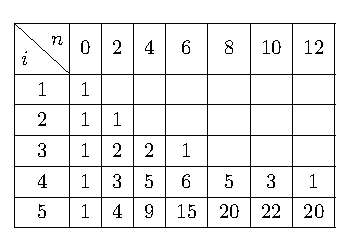
\includegraphics[]{figures/table/table_sing_coh.pdf}   
%    \caption{The singular cohomology $H^{i}(\mathcal{F};\mathbb{C})$ for $\mathcal{F}=\GL_n/B$}    
%\end{table}


$\overline{\Omcell}_w \subseteq \mathcal{F}$ is called the \textbf{Schubert variety}. It is well-known that
$$\overline{\Omcell}_w= \bigsqcup_{w' \leqslant w} \Omcell_w$$
as a set. Especially, for any $s\in W$ with $l(s)=1$, denote $P_s=B \sqcup BsB$,
$$\overline{\Omcell}_s= \Omcell_{\Id} \sqcup \Omcell_s = B/B \sqcup BsB/B = P_s/B \cong \mathbb{P}^1.$$
Most  Schubert varieties are not smooth.


\subsection{$\mathcal{F} \times \mathcal{F}$}\label{subsec:product_of_F}
As a more complicated geometrical object, $\mathcal{F} \times \mathcal{F}$ works as the base space for the Steinberg variety, which turns out to be the central focus in the thesis. $\mathcal{F} \times \mathcal{F}$ has naturally a diagonal $\GL_n$-action:
$$\GL_n \times \mathcal{F} \times \mathcal{F} \longrightarrow \mathcal{F} \times \mathcal{F} \qquad (g,F_1,F_2) \longmapsto (gF_1,gF_2).$$
Under this action, $\mathcal{F} \times \mathcal{F}$ has a stratification consisting of $\GL_n$-orbits, indexed by the Weyl group:
$$\GL_n \setminus (\mathcal{F} \times \mathcal{F}) \cong \GL_n \setminus (\GL_n/B \times \GL_n/B) \cong B \setminus \GL_n /B \cong W \quad \text{ as sets.}$$

For $w'\in W$, denote $\OOmcell_{w'}:= \GL_n \cdot (F_{\Id}, F_{w'})$. Then $\mathcal{F} \times \mathcal{F}= \sqcup_{w'} \OOmcell_{w'}$. Moreover, by the orbit-stabilizer theorem, we get
$$\OOmcell_{w'} \cong \GL_n/\left( B \cap w'B(w')^{-1}  \right)$$
which is an $\mathbb{A}^{l(w')}$-bundle over $\mathcal{F}$.
% https://q.uiver.app/?q=WzAsMyxbMCwwLCJcXG1hdGhiYntBfV57bCh3Jyl9IFxcY29uZyBCL1xcbGVmdCggQiBcXGNhcCB3J0IodycpXnstMX0gIFxccmlnaHQpIl0sWzEsMCwiXFxHTF9uL1xcbGVmdCggQiBcXGNhcCB3J0IodycpXnstMX0gIFxccmlnaHQpIl0sWzEsMSwiXFxtYXRoY2Fse0Z9PVxcR0xfbi9CXFxoc3BhY2V7NW1tfSJdLFswLDFdLFsxLDJdXQ==
%\[\begin{tikzcd}
%	{\mathbb{A}^{l(w')} \cong B/\left( B \cap w'B(w')^{-1}  \right)} & {\GL_n/\left( B \cap w'B(w')^{-1}  \right)} \\
%	& {\hspace{-10mm}\mathcal{F}=\GL_n/B}
%	\arrow[from=1-1, to=1-2]
%	\arrow[from=1-2, to=2-2]
%\end{tikzcd}\]

Different from $\mathcal{F}$, the $\GL_n$-action on $\mathcal{F} \times \mathcal{F}$ is not transitive. To facilitate the stratification of $\mathcal{F}\times \mathcal{F}$, we introduce the twisted $\GL_n \times \GL_n$-action:
$$\GL_n \times \GL_n \times \mathcal{F} \times \mathcal{F} \longrightarrow \mathcal{F} \times \mathcal{F} \qquad (g_1,g_2,F_g,F_{g'}) \longmapsto (F_{g_1g},F_{g_1(gg_2g^{-1}) g'}).$$
If we write $\underline{F}_{g,g'}:= (F_g,F_{gg'}) \in \mathcal{F} \times \mathcal{F}$, then 
$$(g_1,g_2) \cdot\underline{F}_{g,g'}=\underline{F}_{g_1g,g_2g'}.$$

This $\GL_n \times \GL_n$-action is now transitive, and decomposes $\mathcal{F}\times \mathcal{F}$ as disjoint union of finite many $B \times B$-orbits, which are compatible with $G$-orbits:

\begin{equation*}
\begin{aligned}
  &\OOmcell_{w,w'}:=\; (B \times B) \cdot \underline{F}_{w,w'} \subseteq \mathcal{F}\times \mathcal{F}\\ 
  &\mathcal{F}\times \mathcal{F}= \bigsqcup_{w, w'\in W} \OOmcell_{w,w'} \qquad\OOmcell_{w'}= \bigsqcup_{w\in W} \OOmcell_{w,w'} \\
\end{aligned}
\end{equation*}
\begin{equation}\label{eq:twisted_stabilizer}
\begin{aligned}
   \OOmcell_{w,w'} \cong\;& (B \times B)/\left\{ (g_1,g_2) \in B \times B  \;\middle|\; (g_1,g_2) \cdot (F_w,F_{ww'})=(F_w,F_{ww'})  \right\}\\
=\;& (B \times B)/\left\{ (g_1,g_2) \in B \times B  \;\middle|\; g_1wB=wB, g_1wg_2w'B=ww'B  \right\}\\   
%=\;& (B \times B)/\left\{ (g_1,g_2) \in B \times B  \;\middle|\; g_1wB=wB, (w^{-1}g_1w)g_2w'B=w'B  \right\}\\   
=\;& (B \times B)/\left\{ (g_1,g_2) \in B \times B  \;\middle|\; g_1\in wBw^{-1}, g_2 \in (w^{-1}g_1^{-1}w) \left(w'Bw'^{-1}\right)  \right\}\\  
=\;& (B \times B)/\left\{ (g_1,g_2) \in \left(B \cap wBw^{-1}\right) \times (w^{-1}g_1^{-1}w)  \left(B \cap  w'Bw'^{-1}\right)    \right\}\\  
   \cong\;& B/(B \cap wBw^{-1}) \times B/(B \cap w'Bw'^{-1}) \cong \mathbb{A}^{l(w)+l(w')}
\end{aligned}
\end{equation}
We conclude the information of orbits and fixed points in Table \ref{table:orbit_fixed_points}.

\begin{table}[ht]
	\begin{minipage}[b]{.43\textwidth}
\centering
\[
\begin{array}{c|c|c}
\hline
G    & \text{Orbit}                       & G\text{-fixed points}  \\ \hline
\GL_n & \mathcal{F}          & \varnothing            \\ \hline
B    & \Omcell_w            \\ \hline
T    & -                                  & \{F_w |  \, w \in W \} \\ \hline
\end{array}
\]
\subcaption{$\mathcal{F}$}
	\end{minipage}
	\begin{minipage}[b]{.55\textwidth}
		\centering
		\[
		\begin{array}{c|c|c}
		\hline
		G                  & \text{Orbit}              & G\text{-fixed points}                      \\ \hline
		\GL_n \times \GL_n & \mathcal{F} \times \mathcal{F} & \varnothing                                \\ \hline
		\GL_n              & \OOmcell_{w'}              & \varnothing                                \\ \hline
		B \times B         & \OOmcell_{w,w'}            & \{F_{\Id,\Id} \}                           \\ \hline
		T                  & -                         & \{\underline{F}_{w,w'} |  \, w,w' \in W \} \\ \hline
		\end{array}
		\]
		\subcaption{$\mathcal{F} \times \mathcal{F}$}
	\end{minipage}
\caption{Orbit and fixed points}
\label{table:orbit_fixed_points}
\vspace{3mm}
\end{table}

Like $\mathcal{F}$, we also study the closure of $\OOmcell_{w'}$ and $\OOmcell_{w,w'}$ in special case. It can be shown that 
$$\overline{\OOmcell}_{w'} = \bigsqcup_{x'\leqslant w'} \OOmcell_{x'} \qquad 
\overline{\OOmcell}_{w,w'} = \bigsqcup_{x \leqslant w, x'\leqslant w'} \OOmcell_{x,x'}$$
as a set. Especially, for any $s \in W$ with $l(s)=1$, \footnote{Here, $\GL_n \times^B X$ is called balanced product. Roughly, it is defined by
$$\GL_n \times^B X :=\GL_n \times X/\big( (gb,x) \sim (g,bx) \big)$$
We will discuss balanced product in Subsection \ref{subsec:balanced_product} thoroughly.}

\begin{equation*}
\begin{aligned}
 \overline{\OOmcell}_{s} = \OOmcell_{\Id}\sqcup \OOmcell_{s} \cong\;& 
  \GL_n /(B \cap sBs^{-1}) &&\sqcup \GL_n/B \\ 
  \cong\;&  \GL_n \times^{B} \left(B/(B \cap sBs^{-1})\right)\hspace{-0.4cm} &&\sqcup \GL_n \times^{B} (B/B) \\ 
  \cong\;& \GL_n \times^{B} (BsB/B) &&\sqcup \GL_n \times^{B} (B/B)  \\ 
  \cong\;& \GL_n \times^{B} (P_s/B)&& \\ 
\end{aligned}
\end{equation*}
is an $\mathcal{F}$-bundle over $\mathbb{P}^1$. Also, 
\begin{equation*}
\begin{aligned}
\overline{\OOmcell}_{\Id,s} = \OOmcell_{\Id,s} \sqcup \OOmcell_{\Id,\Id} \cong\;& 
 \big(B/B \times BsB/B\big) \sqcup \big(B/B \times B/B\big)  \\ 
 \cong\;& P_s/B \cong \mathbb{P}^1
\end{aligned}
\end{equation*}
Other closure can be highly singular.

\begin{eg}
In the Table \ref{table:stratifications_of_FF}, $n=3$, $t=(12)$, $s=(23)$. In this case, $\mathcal{F}\times \mathcal{F}$ has $6$ $\GL_3$-orbits, and each $\GL_3$-orbits decompose as $6$ $B\times B$-orbits, with dimensions equal to $l(w)+l(w')$. 


We can also see the $\GL_3$-orbit (and its closure) from the table, for example,
\begin{equation*}
\begin{aligned}
  \OOmcell_{s}=\;& \OOmcell_{\Id,s} \sqcup
  \OOmcell_{t,s} \sqcup
  \OOmcell_{s,s} \sqcup
  \OOmcell_{ts,s} \sqcup
  \OOmcell_{st,s} \sqcup
  \OOmcell_{sts,s}  \\ 
  \overline{\OOmcell}_{s}=\;& \OOmcell_{s} \sqcup \OOmcell_{\Id} = \bigsqcup_{w} (\OOmcell_{w,s} \sqcup \OOmcell_{w,\Id})
\end{aligned}
\end{equation*}
We color pieces of $\OOmcell_{s}$ by blue, and $\OOmcell_{ts,s}$ by light blue.
\end{eg}



Now we understand the structure a lot about $\mathcal{F}$ and $\mathcal{F} \times \mathcal{F}$, and the whole process will be applied repeatedly in Section \ref{sec:typical_variety} and \ref{sec:stratification}. 
\section{Quivers}
To introduce more complicated spaces and discuss their stratifications, we fix notation related to quiver and algebraic group in the following sections.

Roughly speaking, a quiver is a directed multigraph permitting loops.

\begin{defn}[Quiver]
A quiver is a quadruple 
$$Q=(v(Q),a(Q),s,t)$$
where
\begin{itemize}[noitemsep,topsep=0pt]
\item $v(Q)$ is a non-empty set consisting of vertices of $Q$,
\item $a(Q)$ is a set consisting of arrows of $Q$,
\item $s:a(Q) \longrightarrow v(Q)$ is a map indicating the start vertex of arrows,
\item $t:a(Q) \longrightarrow v(Q)$ is a map indicating the terminal vertex of arrows.
\end{itemize}
\end{defn}

\begin{remark}\label{rmk:quiver_restriction}
In the first part of our master thesis, all the quivers are supposed to be connected and finite (i.e., $v(Q)$, $a(Q)$ are finite sets). We will only encounter disconnected and infinite quiver as Auslander--Reiten quiver later on.
\end{remark}

\begin{eg}
The following graphs are quivers.

\begin{table}[ht]
\centering
\begin{tabular}{@{\extracolsep{5mm}}ccc}
$$\begin{tikzcd}[ampersand replacement=\&]
	\bullet \& \bullet \& \bullet \& \bullet
	\arrow[from=1-1, to=1-2]
	\arrow[from=1-3, to=1-2]
	\arrow[from=1-4, to=1-3]
\end{tikzcd}$$ & $$\begin{tikzcd}[ampersand replacement=\&]
 	\bullet \arrow[out=120,in=60,loop,looseness=8]
 	\arrow[out=0,in=-60,loop,looseness=8]
 	\arrow[out=-120,in=-180,loop,looseness=8]
 \end{tikzcd}$$ & $$\begin{tikzcd}[ampersand replacement=\&]
 	1 \& 2
 	\arrow["a", curve={height=-6pt}, from=1-1, to=1-2]
 	\arrow["b"', curve={height=6pt}, from=1-1, to=1-2]
 \end{tikzcd}$$ \\
 quiver of type $A_3$ & $3$-loop quiver $L(3)$ & $2$-Kronecker quiver $K(2)$
\end{tabular}
\end{table}
The reader can easily read the quadruple of quivers from the graphs. Take $Q=K(2)$ as an example, we have 
$$v(Q)=\{1,2\}, \qquad a(Q)=\{a,b\} \qquad s,t: \{a,b\}\longrightarrow \{1,2\}$$
by $s(a)=s(b)=1$, $t(a)=t(b)=2$.

For simplicity, we mainly use simpler quivers as examples:

\begin{table}[ht]
\centering
\begin{tabular}{@{\extracolsep{5mm}}ccc}
$$\begin{tikzcd}[ampersand replacement=\&]
	\bullet 
\end{tikzcd}$$ & $$\begin{tikzcd}[ampersand replacement=\&]
	\bullet \& \bullet 
	\arrow[from=1-1, to=1-2]
 \end{tikzcd}$$ & $$\begin{tikzcd}[ampersand replacement=\&]
 	\bullet \arrow[out=30,in=-30,loop,looseness=6]
 \end{tikzcd}$$ \\
 trivial quiver & quiver of type $A_1$ & $1$-loop quiver $L(1)$
\end{tabular}
\end{table}

\end{eg}

From those quivers we are able to construct relatively complicated algebraic and geometrical objects.

\begin{defn}[Quiver representation]
Fix a quiver $Q$. 

A representation of $Q$ consists of the following data:
\begin{itemize}[noitemsep,topsep=0pt]
\item A finite dimensional $\mathbb{C}$-vector space $V_i$ for each vertex $i \in v(Q)$;
\item A $\mathbb{C}$-linear map $V_r: V_{s(r)} \longrightarrow V_{t(r)}$ for each arrow $r \in a(Q)$.
\end{itemize}

A morphism $f:V \longrightarrow W$ is a collection of morphisms $f_i: V_i \longrightarrow W_i$ (for every $i \in v(Q)$) which makes the following diagram commute:
% https://q.uiver.app/?q=WzAsNCxbMCwwLCJWX3tzKGEpfSAiXSxbMSwwLCJWX3t0KGEpfSJdLFsxLDEsIldfe3QoYSl9Il0sWzAsMSwiV197cyhhKX0gIl0sWzAsMywiZl97cyhhKX0iLDJdLFswLDEsIlZfYSJdLFsxLDIsImZfe3QoYSl9Il0sWzMsMiwiV19hIl1d
\[\begin{tikzcd}
	{V_{s(r)} } & {V_{t(r)}} \\
	{W_{s(r)} } & {W_{t(r)}}
	\arrow["{f_{s(r)}}"', from=1-1, to=2-1]
	\arrow["{V_r}", from=1-1, to=1-2]
	\arrow["{f_{t(r)}}", from=1-2, to=2-2]
	\arrow["{W_r}", from=2-1, to=2-2]
\end{tikzcd}\]

We denote the category of representations of $Q$ by $\rep(Q)$.
\end{defn}
\begin{eg}\label{eg:1-loop_quiver}
A representation of the $1$-loop quiver $L(1)$ is a $2$-tuple
$$(V, \; \alpha: V \longrightarrow V)$$
which is equivalent to a (finite dimensional) $\mathbb{C}[t]$-module.
\end{eg}
\begin{remark}
The equivalence in Example \ref{eg:1-loop_quiver} can be generalized to arbitrary quivers. For a quiver $Q$, we can define the path algebra $\mathbb{C}Q$, and view any $Q$-representation as $\mathbb{C}Q$-module, and vice versa.
\end{remark}

\begin{defn}[$Q$-vector space/Vector space with quiver partition]\label{def:Q-vs}
Fix a quiver $Q$, a $Q$-vector space is a finite dimensional $\mathbb{C}$-vector space with a direct sum decomposition
$$V= \bigoplus_{i \in v(Q)} V_i.$$
The dimension vector of a $Q$-vector space is defined as
$$\dimv V :=\left( \dim_{\mathbb{C}} V_i \right)_{i \in v(Q)} \in \prod_{i \in v(Q)} \mathbb{Z}.$$
\end{defn} 

On the contrary, given $\dimvec{d} \in \prod_{i \in v(Q)} \mathbb{N}_{\geqslant 0}$, we can construct a canonical $Q$-vector space of dimension vector $\dimvec{d}$, as follows:
$$V= \bigoplus_{i \in v(Q)} V_i \qquad \text{ with } V_i= \mathbb{C}^{\dimvec{d}_i}.$$

\begin{defn}
The total dimension vector of a $Q$-vector space $V$ is defined as
$$\left| \dimv V  \right|:=\dim_{\mathbb{C}} V.$$
For $\dimvec{d} \in \prod_{i \in v(Q)} \mathbb{N}_{\geqslant 0}$, denote $\abdimvec{d}:= \sum_{i \in v(Q)} \dimvec{d}_i$.
\end{defn}
\begin{defn}[Space of representations with given dimension vector]
For any quiver $Q$, dimension vector $\dimvec{d}$, fix the canonical $Q$-vector space $V= \bigoplus_{i \in v(Q)} V_i$, the space of representations with dimension vector $\dimvec{d}$ is defined as
\begin{equation*}
\begin{aligned}
  \Rep_{\dimvec{d}}(Q):=\;&  \left\{ (V_i,V_a: V_{s(a)} \longrightarrow V_{t(a)} ) \text{ as a representation of $Q$}  \right\} \\ 
  =\;& \bigoplus_{r \in a(Q)} \Hom \left(\mathbb{C}^{\dimvec{d}_{s(a)}},\mathbb{C}^{\dimvec{d}_{t(a)}}\right)
\end{aligned}
\end{equation*}

Since we encode the information of vector space in $\dimvec{d}$, $\Rep_{\dimvec{d}}(Q)$ only records the information of linear maps.
\end{defn}

For both $Q$-vector spaces and $Q$-representations, we can define (complete) flags.

\begin{defn}[Flag with quiver] \label{def:flag_with_quiver}
For a quiver representation $V \in \rep(Q)$, a (partial) flag of $V$ is defined as an increasing sequence of subrepresentation of $V$, i.e.,
$$F: 0 \subseteq M_1 \subseteq \ldots \subseteq M_d=V \qquad M_k\in \rep(Q). $$
For a $Q$-vector space $V=\oplus_{i \in v(Q)}V_i$, a (quiver-graded partial) flag of $V$ is defined as an increasing sequence of $Q$-subspace of $V$, i.e.,
$$F: 0 \subseteq M_1 \subseteq \ldots \subseteq M_d=V \qquad M_k=\bigoplus_{i \in v(Q)}M_{k,i}. $$
For both $Q$-vector space and $Q$-representation, $F$ is called a \textbf{complete flag} if $d=\dim_{\mathbb{C}} V$ and
$$\dim_{\mathbb{C}} M_k=k \qquad \text{ for any }k \in \{1,\ldots, d  \}$$
\end{defn}
For the flag we also have the notation of dimension vector.
\begin{defn}[flag-type dimension vector]\label{def:ftdv}
For any flag $F: 0 \subseteq M_1 \subseteq \ldots \subseteq M_d \subseteq V$, the (flag-type) dimension vector of $F$ is defined as
$$\ftdimvec{f}=\big(\!\dimv M_k   \big)_{k \in \{1,\ldots,d\}} \in  \prod_{\substack{i \in v(Q) \\ k \in \{1,\ldots,d\}}} \mathbb{Z}.$$
$\ftdimvec{f}$ is called a complete flag-type dimension vector if $\ftdimvec{f}$ is the dimension vector of some complete flag $F$, i.e.,\footnote{For convenience, we define $M_0:=0$.} $d=\abdimvec{f}$ and
$$\left| \dimv M_{k+1}/M_k \right|=1 \qquad \text{ for any }k \in \{0,\ldots, d-1  \}.$$
\end{defn}
From now on, we denote a complete dimension vector by $\ftdimvec{d}$, and  (partial) dimension vectors by $\ftdimvec{f}$, $\ftdimvec{g}$. 

\begin{eg}\label{eg:5-case-0}
For the quiver $Q: \textcolor{red}{i} \longrightarrow \textcolor{blue}{i'}$, $\dimvec{d}=(3,2)$, the canonical $Q$-vector space of dimension vector $\dimvec{d}$ is
\begin{equation*}
\begin{aligned}
  V=\;& V_i \oplus V_{i'} \\ 
  =\;& \left< v_1,v_2,v_3 \right>_{\mathbb{C}} \oplus \left< v_4,v_5 \right>_{\mathbb{C}}\\ 
\end{aligned}
\end{equation*}
The flag 
$$F: 0 \subseteq \left< v_4 \right>
\subseteq \left< v_4,v_1 \right>
\subseteq \left< v_4,v_1,v_2 \right>
\subseteq \left< v_4,v_1,v_2,v_5 \right>
\subseteq \left< v_4,v_1,v_2,v_5,v_3 \right>=V$$
is a complete flag of $V$, with complete dimension vector
{
\def\arraystretch{0.8}
$$\ftdimvec{d}= \begin{pmatrix}
3,2\\ 2,2 \\ 2,1 \\ 1,1 \\ 0,1
\end{pmatrix}.$$
}
\end{eg}
\begin{remark}
Any complete flag-type dimension vector $\ftdimvec{d}$ can be viewed as a partition of set $\{1,\ldots, \abdimvec{d} \}$, i.e., a map
$$\ptt: \{1,\ldots, \abdimvec{d}  \} \longrightarrow v(Q)$$
such that $\#\ptt^{-1}(i)=\dimvec{d}_i$.\footnote{The partition corresponding to $\ptt$ is$$\{1,\ldots, \abdimvec{d}\}=\bigsqcup_{i \in v(Q)}\ptt^{-1}(i).$$} We color the set $\{1,\ldots, \abdimvec{d}  \}$ by the partition $\ptt$. In the Example \ref{eg:5-case-0},
{
\def\arraystretch{0.8}
$$\ftdimvec{d}= \begin{pmatrix}
3,2\\ 2,2 \\ 2,1 \\ 1,1 \\ 0,1
\end{pmatrix} \quad
\begin{aligned}
&\text{ corresponds to }\quad \{1,2,3,4,5\}= \{2,3,5\} \sqcup \{1,4\}\\
&\text{ corresponds to }\quad 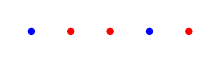
\begin{tikzpicture}
% \vpartition[
% floor=1,
% tkzpic=0,
% type=0
% ]{{5}}
 \tie[color=blue,bull=1,bulletie=0.04,style=solid]{{1,0}}
 \tie[color=red,bull=1,bulletie=0.04,style=solid]{{2,0}}
 \tie[color=red,bull=1,bulletie=0.04,style=solid]{{3,0}}
 \tie[color=blue,bull=1,bulletie=0.04,style=solid]{{4,0}}
 \tie[color=red,bull=1,bulletie=0.04,style=solid]{{5,0}}
 \end{tikzpicture}
\end{aligned}
$$
}
\end{remark}

\section{Symmetric group calculus}

As a reminder, we recall some basic diagrams referring to the elements in $S_n$, and do some calculations by these diagrams. We will also relate cosets with complete flag-type dimension vectors.

Fix a quiver $Q$ and dimension vector $\dimvec{d}$. Later (Definition \ref{def:absalggp}, \ref{def:relalggp}) we will define 
$$\absgp{W}_{\abdimvec{d}}= S_{\abdimvec{d}} \qquad W_{\dimvec{d}} = \prod_{i \in v(Q)} S_{\dimvec{d}_i} \leqslant \absgp{W}_{\abdimvec{d}}$$
For simplicity, we take $v(Q)=\{1,\ldots, k\}$, then $W_{\dimvec{d}}= S_{\dimvec{d}_1} \times \cdots \times S_{\dimvec{d}_k}$ embeds in  $S_{\abdimvec{d}}$.

\begin{remark}
We have different ways to express $\ww \in \absgp{W}_{\abdimvec{d}}= S_{\abdimvec{d}}$. For example, take $\abdimvec{d}=5$, $\ww \in S_5$ by
$$\ww(1)=4,\quad \ww(2)=3,\quad \ww(3)=1,\quad \ww(4)=5,\quad \ww(5)=2,$$ 
then one can represent $\ww$ via
{
\setlength\arraycolsep{1pt}
\renewcommand{\arraystretch}{0.6}
\begin{equation*}
\begin{aligned}
  \ww \hat{=}\;& (14523) \hat{=} \begin{pmatrix}
  1\,2\,3\,4\,5\\ 4\,3\,1\,5\,2
  \end{pmatrix} \hat{=} \parbox[h][][c]{3cm}{\permutation[tkzpic=1]{4,3,1,5,2}}\hspace{-6mm} \hat{=}\begin{bmatrix}
  &&\scriptstyle 1&&\\
  &&&&\scriptstyle 1\\
  &\scriptstyle 1&&&\\
  \scriptstyle 1&&&&\\
  &&&\scriptstyle 1&
  \end{bmatrix} \\ 
  \hat{=}\;& (23)(34)(45)(12)(23)(12) \hat{=} \hspace{0mm} 
  \parbox[h][][c]{3cm}{ 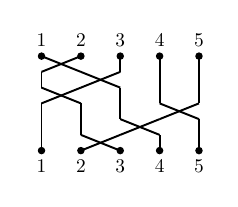
\begin{tikzpicture}
   \permutation[
   height=0.2,
   bullb=0,
   floor=5,
   tkzpic=0,
   type=1
   ]{2,1,3,4,5}
   \permutation[
   height=0.2,
   bulla=0,
   bullb=0,
   floor=4,
   tkzpic=0,
   type=0
   ]{1,3,2,4,5}
   \permutation[
   height=0.2,
   bulla=0,
   bullb=0,
   floor=3,
   tkzpic=0,
   type=0
   ]{2,1,3,4,5}
    \permutation[
    height=0.2,
    bulla=0,
    bullb=0,
    floor=2,
    tkzpic=0,
    type=0
    ]{1,2,3,5,4}
   \permutation[
   height=0.2,
   bulla=0,
   bullb=0,
   floor=1,
   tkzpic=0,
   type=0
   ]{1,2,4,3,5}
   \permutation[
   height=0.2,
   bulla=0,
   floor=0,
   tkzpic=0,
   type=-1
   ]{1,3,2,4,5}
   \end{tikzpicture}}
\end{aligned}
\end{equation*}
}

Even though all expressions give us the same amount of information, the diagram presents them more vividly. For example, each intersection of strands corresponds to a simple reflection, so we read from the diagram that $l(\ww)=6$. Readers can also check that
\begin{equation*}
\begin{aligned}
  &  l(\ww s_1)=5,\quad l(\ww s_2)=5,\quad l(\ww s_3)=7,\quad l(\ww s_4)=5,\\ 
  &  l(s_1\ww)=7,\quad l(s_2\ww)=5,\quad l(s_3\ww)=5,\quad l(s_4\ww)=7,\\ 
\end{aligned}
\end{equation*} 
where $s_i:=(i,i+1) \in S_5$ are simple reflections.

\end{remark}

\begin{defn}[Simple reflections in the Weyl group]
For $i \in \left\{ 1, \ldots , \abdimvec{d}-1 \right\}$, the simple reflection is defined as
$$s_i:=(i,i+1) \in  S_{\abdimvec{d}}.$$
We define
$$\Pi=\;  \Big\{ s_i \in S_{\abdimvec{d}} \;\Big|\; i \in \left\{ 1, \ldots , \abdimvec{d}-1 \right\} \Big\}$$
as the set of simple reflections in $\absgp{W}_{\abdimvec{d}}$, and
\begin{equation*}
\begin{aligned} 
    \Pi_{\dimvec{d}}=\;&  \Big\{ s_i \in S_{\dimvec{d}_1} \times \cdots \times S_{\dimvec{d}_k} \;\Big|\; i \in \left\{ 1, \ldots , \abdimvec{d}-1 \right\} \Big\} \\ 
    =\;&\left\{ s_1,\ldots, s_{\abdimvec{d}-1} \right\} \smallsetminus \left\{s_{\dimvec{d}_1},s_{\dimvec{d}_1+\dimvec{d}_2},\ldots,s_{\dimvec{d}_1+\cdots+\dimvec{d}_{k-1}} \right\} \\
\end{aligned}
\end{equation*}
as the set of simple reflections in $W_{\dimvec{d}}$.
\end{defn}
We also denote  the longest elements in $\absgp{W}_{\abdimvec{d}}$ and  $W_{\dimvec{d}}$ by $\ww_{\max}$ and $w_{\max}$,  respectively. See Table \ref{table:Wgp_collected_notation} for a picture of $\ww_{\max}$ and $w_{\max}$.

We discuss right cosets $W_{\dimvec{d}}\setminus\absgp{W}_{\abdimvec{d}}$ and minimal length coset representatives now.

Multiplying on the left by $w\in W_{\dimvec{d}}$ is equivalent to plugging in a diagram representing $w \in W_{\dimvec{d}}$ underneath the original diagram. Therefore, we connect some bottom points by lines, indicating that switching them will cause no trouble. Furthermore, we color different parts to make the following more explicitly.

\begin{proposition}\label{prop:5-case-0.05}
Every element $W_{\dimvec{d}}\ww \in W_{\dimvec{d}}\setminus\absgp{W}_{\abdimvec{d}}$ corresponds to a partition on set $\left\{ 1, \ldots , \abdimvec{d} \right\}$ (of a given number partition $\dimvec{d}$), which corresponds to a complete flag-type dimension vector $\ftdimvec{d}$, i.e., an ordered set of points colored by the vertices of $Q$.
\end{proposition}

\begin{eg}\label{eg:5-case-0.1}
\begin{equation*}
\begin{aligned}
\parbox[h][][c]{3cm}{
 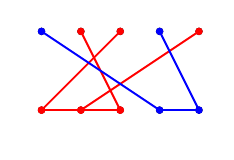
\begin{tikzpicture}
 \vpartition[
 floor=0,
 tkzpic=0,
 type=0
 ]{{5}}
 \tie[color=red,bull=1,bulletie=0.04,style=solid,tieheight=0]{{1},{2},{3}}
 \tie[color=red,bull=1,bulletie=0.04,style=solid]{{3,1},{1,0}}
 \tie[color=red,bull=1,bulletie=0.04,style=solid]{{5,1},{2,0}}
 \tie[color=red,bull=1,bulletie=0.04,style=solid]{{2,1},{3,0}}
 \tie[color=blue,bull=1,bulletie=0.04,style=solid]{{1,1},{4,0},{5,0},{4,1}}
 \end{tikzpicture}
 }
  =\hspace{8mm}& 
\parbox[h][][c]{3cm}{
 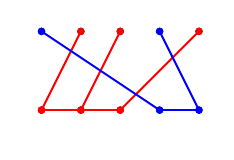
\begin{tikzpicture}
 \vpartition[
 floor=0,
 tkzpic=0,
 type=0
 ]{{5}}
 \tie[color=red,bull=1,bulletie=0.04,style=solid,tieheight=0]{{1},{2},{3}}
 \tie[color=red,bull=1,bulletie=0.04,style=solid]{{2,1},{1,0}}
 \tie[color=red,bull=1,bulletie=0.04,style=solid]{{3,1},{2,0}}
 \tie[color=red,bull=1,bulletie=0.04,style=solid]{{5,1},{3,0}}
 \tie[color=blue,bull=1,bulletie=0.04,style=solid]{{1,1},{4,0},{5,0},{4,1}}
 \end{tikzpicture}
 } \qquad   \text{ in } \Wd\setminus \WWd \\
 since\hspace{5.7cm}&\hspace{10cm}\\
%\shortintertext{since}
\parbox[h][][c]{3cm}{
 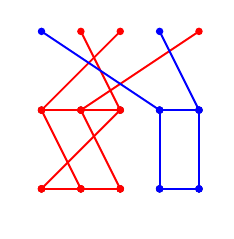
\begin{tikzpicture}
 \vpartition[
 floor=0,
 tkzpic=0,
 type=0
 ]{{5}}
 \tie[color=red,bull=1,bulletie=0.04,style=solid,tieheight=0]{{1},{2},{3}}
 \tie[color=red,bull=1,bulletie=0.04,style=solid]{{2,2},{3,1},{1,0}}
 \tie[color=red,bull=1,bulletie=0.04,style=solid]{{3,2},{1,1},{2,0}}
 \tie[color=red,bull=1,bulletie=0.04,style=solid]{{5,2},{2,1},{3,0}}
 \tie[color=blue,bull=1,bulletie=0.04,style=solid]{{1,2},{4,1},{4,0}}
 \tie[color=blue,bull=1,bulletie=0.04,style=solid]{{4,2},{5,1},{5,0}}
 \tie[color=red,bull=1,bulletie=0.04,style=solid]{{1,1},{2,1},{3,1}} 
 \tie[color=red,bull=1,bulletie=0.04,style=solid]{{1,0},{2,0},{3,0}} 
 \tie[color=blue,bull=1,bulletie=0.04,style=solid]{{4,1},{5,1}}
 \tie[color=blue,bull=1,bulletie=0.04,style=solid]{{4,0},{5,0}}
 \end{tikzpicture}
 }
  =\hspace{8mm}& 
\parbox[h][][c]{3cm}{
 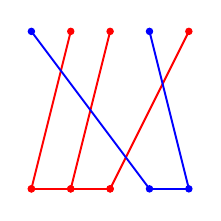
\begin{tikzpicture}
% \vpartition[
% floor=1,
% tkzpic=0,
% type=0
% ]{{5}}
 \tie[color=red,bull=1,bulletie=0.04,style=solid,tieheight=0]{{1},{2},{3}}
 \tie[color=red,bull=1,bulletie=0.04,style=solid]{{2,2},{1,0}}
 \tie[color=red,bull=1,bulletie=0.04,style=solid]{{3,2},{2,0}}
 \tie[color=red,bull=1,bulletie=0.04,style=solid]{{5,2},{3,0}}
 \tie[color=blue,bull=1,bulletie=0.04,style=solid]{{1,2},{4,0},{5,0},{4,2}} 
 \end{tikzpicture}
 } \qquad   \text{ in } \WWd \\
 \end{aligned}
 \end{equation*}

This coset corresponds to the partition $\{1,2,3,4,5 \}= \{2,3,5\} \sqcup \{1,4\}$, and this corresponds to the ordered set of colored points:$\;$ $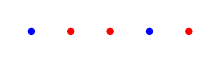
\begin{tikzpicture}
% \vpartition[
% floor=1,
% tkzpic=0,
% type=0
% ]{{5}}
 \tie[color=blue,bull=1,bulletie=0.04,style=solid]{{1,0}}
 \tie[color=red,bull=1,bulletie=0.04,style=solid]{{2,0}}
 \tie[color=red,bull=1,bulletie=0.04,style=solid]{{3,0}}
 \tie[color=blue,bull=1,bulletie=0.04,style=solid]{{4,0}}
 \tie[color=red,bull=1,bulletie=0.04,style=solid]{{5,0}}
 \end{tikzpicture}$

\end{eg}

It is easy to see from the diagram that in every coset, there exists a unique element $u \in \absgp{W}_{\abdimvec{d}}$ of minimal length. Let $\MinWd$ be the collection of these minimal  length coset representatives.\footnote{In some references $\MinWd$ is also denoted by $\Shuffled$, since those elements can be thought as ways off riffle shuffling several words together.}

\begin{proposition}
For any $\ww \in \absgp{W}_{\abdimvec{d}}$, there exists unique $w \in \Wd$, $u \in \MinWd$ such that $\ww=wu$. 
\end{proposition}
\begin{proposition}
For $u \in \MinWd$, $s_i \in \Pi$,
\begin{equation*}
\begin{aligned}
us_iu^{-1}\in W_{\dimvec{d}} \quad\Longrightarrow&\quad us_iu^{-1}=s_{u(i)} \in \Pi_{\dimvec{d}},\\
us_iu^{-1}\notin W_{\dimvec{d}} \quad\Longrightarrow&\quad us_i \in \MinWd.
\end{aligned}
\end{equation*}
\end{proposition}

We finish this section with figures and examples.
% https://q.uiver.app/?q=WzAsOSxbMywwLCJcXE1pbldkIl0sWzMsMSwiV197XFxkaW12ZWN7ZH19XFxzZXRtaW51c1xcYWJzZ3B7V31fe1xcYWJkaW12ZWN7ZH19Il0sWzIsMSwiXFxhYnNncHtXfV97XFxhYmRpbXZlY3tkfX0iXSxbNCwxLCIwIl0sWzEsMSwiV197XFxkaW12ZWN7ZH19Il0sWzAsMSwiMCJdLFs2LDAsInUiXSxbNSwxLCJcXHd3PXd1Il0sWzYsMSwiXFxmdGRpbXZlY3tkfSJdLFswLDEsIlxcY29uZyJdLFswLDIsIiIsMix7InN0eWxlIjp7InRhaWwiOnsibmFtZSI6Imhvb2siLCJzaWRlIjoiYm90dG9tIn19fV0sWzIsMV0sWzEsM10sWzQsMl0sWzUsNF0sWzcsOCwiIiwwLHsic3R5bGUiOnsidGFpbCI6eyJuYW1lIjoibWFwcyB0byJ9fX1dLFs2LDgsIiIsMix7InN0eWxlIjp7InRhaWwiOnsibmFtZSI6Im1hcHMgdG8ifX19XV0=
%\[\begin{tikzcd}
%	&&& \MinWd &&& u \\
%	0 & {W_{\dimvec{d}}} & {\absgp{W}_{\abdimvec{d}}} & {W_{\dimvec{d}}\setminus\absgp{W}_{\abdimvec{d}}} & 0 & {\ww=wu} & {\ftdimvec{d}}
%	\arrow["\cong", from=1-4, to=2-4]
%	\arrow[hook', from=1-4, to=2-3]
%	\arrow[from=2-3, to=2-4]
%	\arrow[from=2-4, to=2-5]
%	\arrow[from=2-2, to=2-3]
%	\arrow[from=2-1, to=2-2]
%	\arrow[maps to, from=2-6, to=2-7]
%	\arrow[maps to, from=1-7, to=2-7]
%\end{tikzcd}\]

\begin{eg}\label{eg:5-case-1}
In Table \ref{table:Wgp_collected_notation}, $\abdimvec{d}=5$, $\dimvec{d}=(3,2)$, typical elements would be
$$\ww = \parbox[h][][c]{3cm}{\permutation[tkzpic=1,type=0]{4,3,1,5,2}} \quad
w =\parbox[h][][c]{3cm}{\permutation[tkzpic=1,type=0]{3,1,2,5,4}} \quad
u =\parbox[h][][c]{3cm}{
 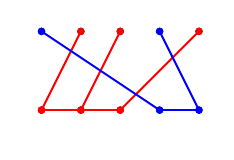
\begin{tikzpicture}
 \vpartition[
 floor=0,
 tkzpic=0,
 type=0
 ]{{5}}
 \tie[color=red,bull=1,bulletie=0.04,style=solid,tieheight=0]{{1},{2},{3}}
 \tie[color=red,bull=1,bulletie=0.04,style=solid]{{2,1},{1,0}}
 \tie[color=red,bull=1,bulletie=0.04,style=solid]{{3,1},{2,0}}
 \tie[color=red,bull=1,bulletie=0.04,style=solid]{{5,1},{3,0}}
 \tie[color=blue,bull=1,bulletie=0.04,style=solid]{{1,1},{4,0},{5,0},{4,1}}
 
 \end{tikzpicture}
 } \quad  $$
 {
 
 %https://tex.stackexchange.com/questions/394775/vertical-space-distribution-when-arraystretch-is-increased
\def\arraystretch{2}
 \begin{table}[ht]
 $$
 \begin{array}{l|l|r|c}
 \hline
 \multicolumn{1}{c|}{\text{set}} & \multicolumn{1}{c|}{\text{element}} & \multicolumn{1}{c|}{\text{special element}} & \text{others/alias} \\ \hline
\absgp{W}_{\abdimvec{d}} = S_5 & \ww,x                               &   \ww_{\max}=  \lbox{\parbox[h][][c]{1.5cm}{\permutation[tkzpic=1,type=0,scale=0.5]{5,4,3,2,1}}  }                                      &   \Pi_{\phantom{d}}=\{s_1,s_2,s_3,s_4 \}            \\ \hline
W_{\dimvec{d}} = S_3 \times S_2      & w                                   &     w_{\max}= \lbox{\parbox[h][][c]{1.5cm}{\permutation[tkzpic=1,type=0,scale=0.5]{3,2,1,5,4}}    }                                    &  \Pi_{\dimvec{d}}=\{s_1,s_2,\phantom{s_3,}s_4 \}              \\ \hline
W_{\dimvec{d}}\setminus\absgp{W}_{\abdimvec{d}} \cong (S_3 \times S_2) \setminus S_5 & \ww, \ftdimvec{d}                   &          \parbox[h][][c]{1.6cm}{\parbox[h][][c]{1.5cm}{ 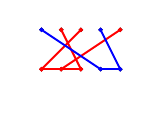
\begin{tikzpicture}[scale=0.5]
 \vpartition[
 floor=0,
 tkzpic=0,
 type=0
 ]{{5}}
 \tie[color=red,bull=1,bulletie=0.04,style=solid,tieheight=0]{{1},{2},{3}}
 \tie[color=red,bull=1,bulletie=0.04,style=solid]{{3,1},{1,0}}
 \tie[color=red,bull=1,bulletie=0.04,style=solid]{{5,1},{2,0}}
 \tie[color=red,bull=1,bulletie=0.04,style=solid]{{2,1},{3,0}}
 \tie[color=blue,bull=1,bulletie=0.04,style=solid]{{1,1},{4,0},{5,0},{4,1}}
 \end{tikzpicture}} }                                   &    \Compd           \\ \hline
\MinWd =\left\{\parbox[h][][c]{1.5cm}{ 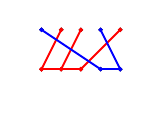
\begin{tikzpicture}[scale=0.5]
 \vpartition[
 floor=0,
 tkzpic=0,
 type=0
 ]{{5}}
 \tie[color=red,bull=1,bulletie=0.04,style=solid,tieheight=0]{{1},{2},{3}}
 \tie[color=red,bull=1,bulletie=0.04,style=solid]{{2,1},{1,0}}
 \tie[color=red,bull=1,bulletie=0.04,style=solid]{{3,1},{2,0}}
 \tie[color=red,bull=1,bulletie=0.04,style=solid]{{5,1},{3,0}}
 \tie[color=blue,bull=1,bulletie=0.04,style=solid]{{1,1},{4,0},{5,0},{4,1}}
 \end{tikzpicture}}  ,\ldots \right\}  & u                                   &                                       \parbox[h][][c]{1.5cm}{ 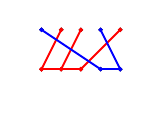
\begin{tikzpicture}[scale=0.5]
 \vpartition[
 floor=0,
 tkzpic=0,
 type=0
 ]{{5}}
 \tie[color=red,bull=1,bulletie=0.04,style=solid,tieheight=0]{{1},{2},{3}}
 \tie[color=red,bull=1,bulletie=0.04,style=solid]{{2,1},{1,0}}
 \tie[color=red,bull=1,bulletie=0.04,style=solid]{{3,1},{2,0}}
 \tie[color=red,bull=1,bulletie=0.04,style=solid]{{5,1},{3,0}}
 \tie[color=blue,bull=1,bulletie=0.04,style=solid]{{1,1},{4,0},{5,0},{4,1}}
 \end{tikzpicture}}      &   \Shuffled            \\ \hline
 \end{array}
 $$
 \caption{Collected notation in $(3,2)$-case}
 \label{table:Wgp_collected_notation}
 \end{table}
 }
 %调整表格。。。大难题
\end{eg}

\begin{eg}\label{eg:3-case-1}
In Table \ref{table:smalleg_Weyl}, 
$$\abdimvec{d}=3,\quad \dimvec{d}=(1,2),\qquad \WWd=S_3,\quad \Wd=S_1 \times S_2,\qquad s=(12),\quad t=(23).$$ The columns ``order of basis" and ``Borel subgroups" will be introduced in Definition \ref{def:special_flags} and Remark \ref{rmk:Borel_difference}.

\begin{table}[ht]
  \vspace{0cm}
    \centering  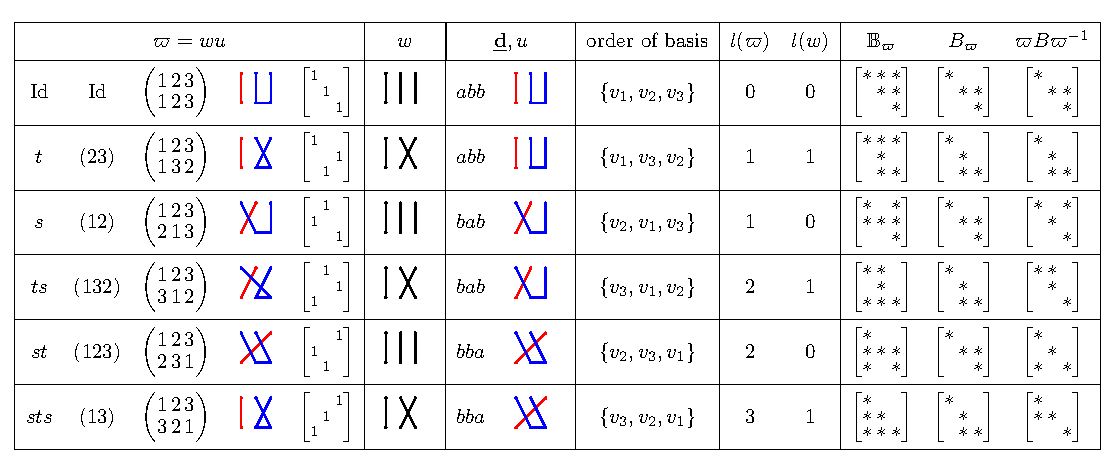
\includegraphics[width=15cm]{figures/table/table_basic_information.pdf}
      \caption{Basic information of $(1,2)$-case}  
      \label{table:smalleg_Weyl} 
      \vspace{3mm}    
        \end{table}       
\end{eg}
\section{Algebraic groups and Lie algebras}\label{sec:algebraic_group_Lie_algebra}
In this section we fix notation for some algebraic groups and Lie algebras. 

\begin{setting}\label{set:Qvs}
Fix a quiver $Q$, a dimension vector $\dimvec{d}$ and a $Q$-vector space 
$$V=\bigoplus_{i \in v(Q)} V_i \qquad \text{with } V_i=\mathbb{C}^{\dimvec{d}_i}.$$
When a basis of $V$ is needed, we fix a total order on $v(Q)$, and denote
$$V=\left< v_1, \ldots v_{\abdimvec{d}} \right> $$
where
$$V_i=\left< v_{f_i+1}, \ldots v_{f_i+\dimvec{d}_i} \right> \qquad f_i= \sum_{i' < i} \dimvec{d}_{i'}.$$
\end{setting}

\subsection{Algebraic groups}

\begin{defn}[Absolute algebraic groups]\label{def:absalggp}
%The following algebraic groups are not related to the quiver partition of $V$.
We set
$$\absgp{G}_{\abdimvec{d}}:= \GL(V)=\GL_{\abdimvec{d}}(\mathbb{C}),$$
and $\absgp{B}_{\abdimvec{d}}$, $\absgp{T}_{\abdimvec{d}}$, $\absgp{N}_{\abdimvec{d}}$ are corresponding standard Borel, torus and unipotent subgroups, respectively.

The Weyl group is
$$\absgp{W}_{\abdimvec{d}}:= N_{\absgp{G}_{\abdimvec{d}}}(\absgp{T}_{\abdimvec{d}})/\absgp{T}_{\abdimvec{d}} \cong S_{\abdimvec{d}}.$$

For $\ww \in \absgp{W}_{\abdimvec{d}}$, we define\footnote{As usual, we abuse the notation of $\ww$ and its lift.}
$$\absgp{B}_{\ww}:= \ww \absgp{B}_{\abdimvec{d}} \ww^{-1}.$$
We will view $\absgp{B}_{\ww}$ as the stabilizer of the flag $F_{\ww}$ with $\absgp{G}_{\abdimvec{d}}$-action.
\end{defn}

\begin{defn}[Relative algebraic groups]\label{def:relalggp}

We set
$$G_{\dimvec{d}}:= \prod_{i \in v(Q)}\GL(V_i)=\prod_{i \in v(Q)}\GL_{\dimvec{d}_i}(\mathbb{C}) \subseteq \absgp{G}_{\abdimvec{d}},$$
and $B_{\dimvec{d}}$, $T_{\dimvec{d}}$, $N_{\dimvec{d}}$ are corresponding standard Borel, torus and unipotent subgroups.

The Weyl group is
$$W_{\dimvec{d}}:= N_{G_{\dimvec{d}}}(T_{\dimvec{d}})/T_{\dimvec{d}} \cong \prod_{i \in v(Q)}S_{\dimvec{d}_i}.$$

For $\ww=wu \in W_{\dimvec{d}}$, we define
$$B_{\ww}:= w B_{\dimvec{d}} w^{-1}.$$
We will view $B_{\ww}$ as the stabilizer of the flag $F_{\ww}$ with $G_{\dimvec{d}}$-action.
\end{defn}

\begin{remark}\label{rmk:Borel_difference}
Be careful that $B_{\ww} \neq \ww B_{\dimvec{d}} \ww^{-1}$. Actually,
$$B_{\ww}= \ww \absgp{B}_{\abdimvec{d}}\ww^{-1} \cap G_{\dimvec{d}}=wB_{\dimvec{d}}w^{-1}$$
The difference is clearly shown in Table \ref{table:smalleg_Weyl}.
\end{remark}

We also have a series of algebraic groups indexed by elements in the Weyl group:
\begin{defn}[More algebraic groups]
For $\ww, \ww'' \in \absgp{W}_{\abdimvec{d}}$, define
\begin{equation*}
\begin{aligned}
  N_{\ww}:=\;& R_u(B_{\ww}),  \\ 
  N_{\ww,\ww''}:=\;& N_{\ww} \cap N_{\ww''},  \\ 
  M_{\ww,\ww''}:=\;& N_{\ww}/N_{\ww,\ww''},  \\ 
\end{aligned}
\end{equation*}
where $R_u$ denotes the unipotent radical.

For $s \in \Pi$ such that $\ww s \ww^{-1} \in W_d$ (i.e., $W_{\dimvec{d}}\ww=W_{\dimvec{d}}\ww s$), define
\begin{equation*}
\begin{aligned}
  P_{\ww,\ww s}:\xlongequal{\ww =wu}\;& w\left( B_{\dimvec{d}} usu^{-1} B_{\dimvec{d}} \cup B_{\dimvec{d}} \right)w^{-1} \\ 
  \xlongequal{\phantom{\ww =wu}}\;&  B_{\ww} \ww s\ww^{-1} B_{\ww} \cup B_{\ww}  \\ 
\end{aligned}
\end{equation*}
\end{defn}
\begin{remark}
One can easily show that $N_{\ww, \ww s}=R_u (P_{\ww, \ww s})$.
\end{remark}
%problems on making short vertical space
%https://tex.stackexchange.com/questions/183562/how-to-reduce-vertical-space-in-matrix?newreg=ca78ba434426423a8be8ce4f1df4548c
%https://tex.stackexchange.com/questions/643384/horizontal-spacing-bmatrix-in-align-environment
%https://tex.stackexchange.com/questions/275725/adjusting-separation-between-matrix-entries
{\setlength\arraycolsep{1pt}
\renewcommand{\arraystretch}{0.6}

%small fonts: use \scriptstyle instead of \scriptsize

%vertical line:
%https://tex.stackexchange.com/questions/33519/vertical-line-in-matrix-using-latexit

\makeatletter
\renewcommand*\env@matrix[1][*\c@MaxMatrixCols c]{%
  \hskip -\arraycolsep
  \let\@ifnextchar\new@ifnextchar
  \array{#1}}
\makeatother
\begin{eg}[Follows Example \ref{eg:5-case-1}] \label{eg:5-case-2}
For $\abdimvec{d}=5$, $\dimvec{d}=(3,2)$, $\ww =\hspace{-3mm} \parbox[h][][c]{2cm}{\permutation[tkzpic=1,type=0,scale=0.5]{4,3,1,5,2}}$\hspace{-7mm}, 
$w =\hspace{-3mm}\parbox[h][][c]{2cm}{\permutation[tkzpic=1,type=0,scale=0.5]{3,1,2,5,4}}$\hspace{-7mm}, $s=s_2$, we compute all the algebraic groups we mentioned:
\begin{equation*}
\begin{aligned}
  &\absgp{G}_{\abdimvec{d}}= \begin{pmatrix}
  * & * & * & * & * \\
  * & * & * & * & * \\
  * & * & * & * & * \\
  * & * & * & * & * \\
  * & * & * & * & * \\
  \end{pmatrix}&
  \absgp{B}_{\abdimvec{d}}=
  \begin{pmatrix}
  * & * & * & * & * \\
   & * & * & * & * \\
   &  & * & * & * \\
   &  &  & * & * \\
   &  &  &  & * \\
  \end{pmatrix}&&
  \absgp{T}_{\abdimvec{d}}=
  \begin{pmatrix}
  * &  &  &  &  \\
   & * &  &  &  \\
   &  & * &  &  \\
   &  &  & * &  \\
   &  &  &  & * \\
  \end{pmatrix}&&
  \absgp{N}_{\abdimvec{d}}=
  \begin{pmatrix}
  \scriptstyle 1 & * & * & * & * \\
   & \scriptstyle 1 & * & * & * \\
   &  & \scriptstyle 1 & * & * \\
   &  &  & \scriptstyle 1 & * \\
   &  &  &  & \scriptstyle 1 \\
  \end{pmatrix}
    \\
  &\absgp{W}_{\abdimvec{d}}\cong S_5&
  \absgp{B}_{\ww}=
   \begin{pmatrix}
  * & * &  &  & * \\
   & * &  &  &  \\
  * & * & * &  & * \\
  * & * & * & * & * \\
   & * &  &  & * \\
  \end{pmatrix}&&
  \absgp{B}_{\ww s}=
     \begin{pmatrix}
    * & * & *  &  & * \\
     & * &  &  &  \\
     & * & * &  & * \\
    * & * & * & * & * \\
     & * &  &  & * \\
    \end{pmatrix}&&
  \\
  &G_{\dimvec{d}}\;=
  \begin{pmatrix}[ccc|cc]
  * & * & * &  &  \\
  * & * & * &  &  \\
  * & * & * &  &  \\
     \hline
   &  &  & * & * \\ 
   &  &  & * & * \\ 
  \end{pmatrix}&
  B_{\dimvec{d}}=
    \begin{pmatrix}[ccc|cc]
    * & * & * &  &  \\
     & * & * &  &  \\
     &  & * &  &  \\
        \hline
     &  &  & * & * \\ 
     &  &  &  & * \\ 
    \end{pmatrix}&&
  T_{\dimvec{d}}=
    \begin{pmatrix}[ccc|cc]
     * &  &  &  &  \\
       & * &  &  &  \\
       &  & * &  &  \\
          \hline
       &  &  & * &  \\
       &  &  &  & * \\
    \end{pmatrix}&&
  N_{\dimvec{d}}=
         \begin{pmatrix}[ccc|cc]
          \scriptstyle 1 & * & * &  &  \\
           & \scriptstyle 1 & * &  &  \\
           &  & \scriptstyle 1 &  &  \\
              \hline
           &  &  & \scriptstyle 1 & * \\ 
           &  &  &  & \scriptstyle 1 \\ 
          \end{pmatrix}  
  \\
&W_{\dimvec{d}}\cong S_3 \times S_2&
  B_{\ww}=
   \begin{pmatrix}[ccc|cc]
  * & * &  &  &  \\
   & * &  &  &  \\
  * & * & * &  &  \\
     \hline
   &  &  & * &  \\
   &  &  & * & * \\
  \end{pmatrix}&&
  B_{\ww s}=
     \begin{pmatrix}[ccc|cc]
  * &  &  &  &  \\
  * & * &  &  &  \\
  * & * & * &  &  \\
     \hline
   &  &  & * &  \\
   &  &  & * & * \\
    \end{pmatrix}&&
  \\
   &N_{\ww}=
    \begin{pmatrix}[ccc|cc]
   \scriptstyle 1 & * &  &  &  \\
    & \scriptstyle 1 &  &  &  \\
   * & * & \scriptstyle 1 &  &  \\
      \hline
    &  &  & \scriptstyle 1 &  \\
    &  &  & * & \scriptstyle 1 \\
   \end{pmatrix}&
   N_{\ww,\ww s}=
      \begin{pmatrix}[ccc|cc]
   \scriptstyle 1 &  &  &  &  \\
    & \scriptstyle 1 &  &  &  \\
   * & * & \scriptstyle 1 &  &  \\
      \hline
    &  &  & \scriptstyle 1 &  \\
    &  &  & * & \scriptstyle 1 \\
     \end{pmatrix}&& 
   M_{\ww,\ww s}=
      \begin{pmatrix}[ccc|cc]
   \scriptstyle 1 & * &  &  &  \\
    & \scriptstyle 1 &  &  &  \\
   \scriptstyle- & \scriptstyle- & \scriptstyle 1 &  &  \\
      \hline
    &  &  & \scriptstyle 1 &  \\
    &  &  & \scriptstyle- & \scriptstyle 1 \\
     \end{pmatrix}&& 
   P_{\ww,\ww s}=
      \begin{pmatrix}[ccc|cc]
   * & * &  &  &  \\
   * & * &  &  &  \\
   * & * & * &  &  \\
   \hline
    &  &  & * &  \\
    &  &  & * & * \\
     \end{pmatrix}
\end{aligned}
\end{equation*}




\end{eg}
}
\subsection{Lie algebra}
We use Fraktur-font symbols to represent the Lie algebras of the corresponding algebraic groups introduced in the last section:
\begin{equation*}
\begin{aligned}
  & \boldsymbol{\mathfrak{g}}_{\abdimvec{d}}, &&\boldsymbol{\mathfrak{b}}_{\abdimvec{d}}, &&\boldsymbol{\mathfrak{t}}_{\abdimvec{d}}, &&\boldsymbol{\mathfrak{n}}_{\abdimvec{d}}, &&\boldsymbol{\mathfrak{b}}_{\ww}  \\
  & \mathfrak{g}_{\dimvec{d}},
  &&\mathfrak{b}_{\dimvec{d}},
  &&\mathfrak{t}_{\dimvec{d}},
  &&\mathfrak{n}_{\dimvec{d}},
  &&\mathfrak{b}_{\ww},\\
  & \mathfrak{n}_{\ww},\hspace{5mm}
  &&\mathfrak{n}_{\ww,\ww''},
  &&\mathfrak{m}_{\ww,\ww''},
  &&\mathfrak{p}_{\ww,\ww s},
  &&\\
\end{aligned}
\end{equation*}

We also have to encode the information of representations as Lie algebra. Notice that
$$\Hom (V_{s(a)},V_{t(a)}) \hookrightarrow \Hom(V,V) \cong \boldsymbol{\mathfrak{g}}_{\abdimvec{d}} \qquad f \longmapsto \iota_{t(a)} \circ f \circ \pi_{s(a)}$$
realizes $\Hom (V_{s(a)},V_{t(a)})$ as a subspace of $\boldsymbol{\mathfrak{g}}_{\abdimvec{d}}$, so 
$$  \Rep_{\dimvec{d}}(Q)= \bigoplus_{r \in a(Q)} \Hom \left(\mathbb{C}^{\dimvec{d}_{s(a)}},\mathbb{C}^{\dimvec{d}_{t(a)}}\right) \subseteq \bigoplus_{r \in a(Q)} \boldsymbol{\mathfrak{g}}_{\abdimvec{d}}.$$
\begin{defn}[Lie algebras connected with representations]\label{def:Lie_alg_with_rep}
For $\ww \in \absgp{W}_{\abdimvec{d}}$, denote 
$$V_{\ww,k}:= \left< e_{\ww(1)},\ldots e_{\ww(k)} \right> \subseteq V.$$
We define Lie subalgebras of $\Rep_{\dimvec{d}}(Q)$ as follows.
%https://tex.stackexchange.com/questions/352752/align-inside-left-right
$$\mathfrak{r}_{\ww}:=\; \left\{ (f_a)_{a\in a(Q)} \in \Rep_{\dimvec{d}}(Q) \;\middle| \; f_a(V_{\ww,k} \cap V_{s(a)}) \subseteq V_{\ww,k} \text{ for any } k \right\},$$
\vspace{-8mm}
\begin{equation*}
\begin{aligned}
  \mathfrak{r}_{\ww,\ww''}:=\;& \mathfrak{r}_{\ww} \cap \mathfrak{r}_{\ww''},  \\ 
  \mathfrak{d}_{\ww,\ww''}:=\;& \mathfrak{r}_{\ww}/\mathfrak{r}_{\ww,\ww''},  \\ 
\end{aligned}
\end{equation*}

\end{defn}
\begin{eg}[Follows Example \ref{eg:5-case-2}]\label{eg:5-case-3}
Consider the quiver $\begin{tikzcd}[ampersand replacement=\&]
	\textcolor{red}{\bullet} \& \textcolor{blue}{\bullet} 
	\arrow[from=1-1, to=1-2]
 \end{tikzcd}$, and $u =\parbox[h][][c]{2cm}{
  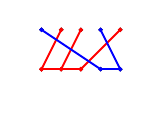
\begin{tikzpicture}[scale=0.5]
  \vpartition[
  floor=0,
  tkzpic=0,
  type=0
  ]{{5}}
  \tie[color=red,bull=1,bulletie=0.04,style=solid,tieheight=0]{{1},{2},{3}}
  \tie[color=red,bull=1,bulletie=0.04,style=solid]{{2,1},{1,0}}
  \tie[color=red,bull=1,bulletie=0.04,style=solid]{{3,1},{2,0}}
  \tie[color=red,bull=1,bulletie=0.04,style=solid]{{5,1},{3,0}}
  \tie[color=blue,bull=1,bulletie=0.04,style=solid]{{1,1},{4,0},{5,0},{4,1}}
  
  \end{tikzpicture}
  }$\hspace{-7mm}. Table \ref{table:Lie_alg} gives us an example of the shape of these Lie algebras. Symbols like $\frac{e_1}{e_2}$ will be explained in Example \ref{eg:K-initial-2}.
\begin{table}[ht]
  \vspace{0cm}
    \centering  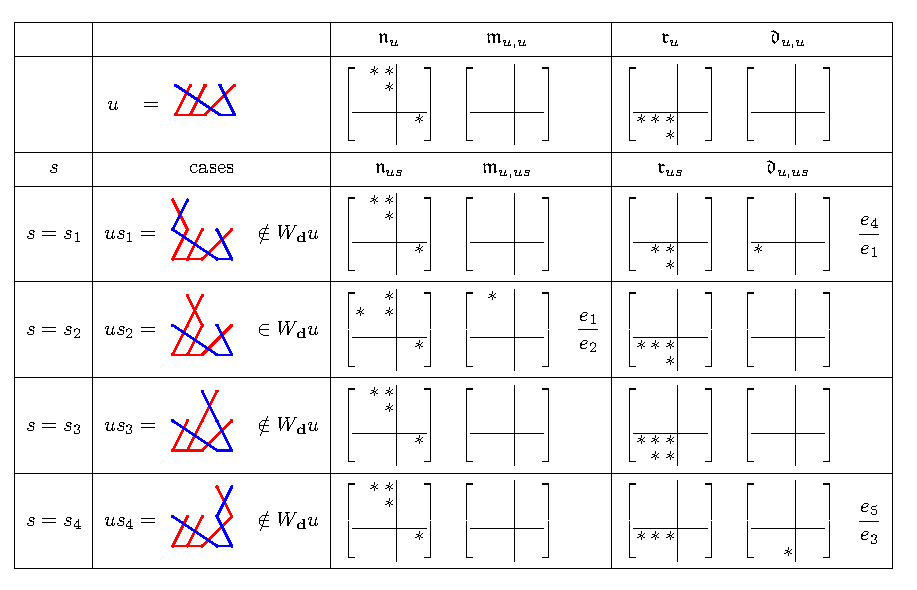
\includegraphics[width=15cm]{figures/table/table_Lie_alg.pdf}
      \caption{examples of Lie algebras}
      \label{table:Lie_alg}        
\end{table}
\end{eg}


\begin{remark}
We also have twisted notation for Lie algebras. For example,
\begin{equation*}
\begin{aligned}
  \underline{\mathfrak{n}}_{\ww,\ww'}=\;& \mathfrak{n}_{\ww,\ww\ww'},
   &&\underline{\mathfrak{m}}_{\ww,\ww'}=\; \mathfrak{m}_{\ww,\ww\ww'},
   &&
   \underline{\mathfrak{p}}_{\ww,s}=\; \mathfrak{p}_{\ww,\ww s}, \\ 
  \underline{\mathfrak{r}}_{\ww,\ww'}=\;& \mathfrak{r}_{\ww,\ww\ww'},
  &&\underline{\mathfrak{d}}_{\ww,\ww'}=\; \mathfrak{d}_{\ww,\ww\ww'}.&&  \\ 
\end{aligned}
\end{equation*}
Another twist happens when we add minus sign as the superscript:
\begin{equation*}
\begin{aligned}
  \boldsymbol{\mathfrak{b}}_{\ww}^{-} =&\boldsymbol{\mathfrak{b}}_{\ww_{\max}\ww},&& \\
  \mathfrak{b}_{\ww}^{-}=&\mathfrak{b}_{w_{\max}\ww}, & 
\mathfrak{n}_{\ww}^{-}=&\mathfrak{n}_{w_{\max}\ww}, \\
  \mathfrak{n}_{\ww,\ww''}^{-}=&\mathfrak{n}_{w_{\max}\ww,w_{\max}\ww''}, & 
\mathfrak{m}_{\ww,\ww''}^{-}=&\mathfrak{m}_{w_{\max}\ww,w_{\max}\ww''}.  \\
\end{aligned}
\end{equation*}
\end{remark}
\section{Quiver flag varieties}\label{sec:typical_variety}

In this section, we define quiver flag varieties we care about in the same spirit as Section \ref{sec:inital_case}. Their stratifications and related ``Schubert" varieties will be defined in Section \ref{sec:stratification}.

Recall Setting \ref{sec:inital_case} and Definition \ref{def:flag_with_quiver}.
\subsection{Flag variety}
\begin{defn}[Absolute complete flag variety]
The absolute complete flag variety $\mathcal{F}_{\abdimvec{d}}$ is defined as 
\begin{align*}
  \mathcal{F}_{\abdimvec{d}}=\;& \absgp{G}_{\abdimvec{d}}/\absgp{B}_{\abdimvec{d}} \\ 
    \cong\;&  \left\{ \text{complete flags of } \mathbb{C}^{\abdimvec{d}} \right\} \\ 
      =\;& \left\{ 0 \subseteq M_1 \subseteq M_2 \subseteq \cdots \subseteq M_{\abdimvec{d}} = \mathbb{C}^{\abdimvec{d}} \;\middle|\; \dim M_k =k \right\} \\ 
       \cong\;&  \left\{ \text{Borel subgroups of } \absgp{G}_{\abdimvec{d}} \right\} \\
          =\;& \left\{ g\absgp{B}_{\abdimvec{d}}g^{-1} \;\middle|\; g \in \absgp{G}_{\abdimvec{d}} \right\} \\ 
\end{align*}
Here, $M_i$ can have no $Q$-vector space structure.
\end{defn}

\begin{defn}[complete flag variety with flag-type dimension vector]
For a complete flag-type dimension vector $\ftdimvec{d}$, the flag variety $\mathcal{F}_{\ftdimvec{d}}$ is defined as
\begin{equation*}
\begin{aligned}
  \mathcal{F}_{\ftdimvec{d}}=\;&  \left\{ \text{complete flags of } V=\raisebox{1.3mm}{$\displaystyle\bigoplus_{i \in v(Q)}$} V_i \text{ with dimension vector } \ftdimvec{d}\right\} \\ 
      =\;& \left\{ F: 0 \subseteq M_1 \subseteq M_2 \subseteq \cdots \subseteq M_{\abdimvec{d}} = V \;\middle|\; \dimv F =\ftdimvec{d} \phantom{\Big)\!\!\!} \right\}
\end{aligned}
\end{equation*}
\end{defn}

\begin{defn}[Relative complete flag variety]
The relative complete flag variety $\mathcal{F}_{\dimvec{d}}$ is defined as 
\begin{equation*}
\begin{aligned}
  \mathcal{F}_{\dimvec{d}}=\;&  \left\{ \text{complete flags of } V=\raisebox{1.3mm}{$\displaystyle\bigoplus_{i \in v(Q)}$} V_i \right\} \\ 
      =\;& \left\{ 0 \subseteq M_1 \subseteq M_2 \subseteq \cdots \subseteq M_{\abdimvec{d}} = V \;\middle|\; \left|\dimv M_k \right| =k \phantom{\Big)\!\!\!} \right\}\\
      =\;& \bigsqcup_{\ftdimvec{d}}\mathcal{F}_{\ftdimvec{d}}
\end{aligned}
\end{equation*}
Here, $M_i$ are $Q$-vector spaces.
\end{defn}

\begin{remark}\label{rmk:action_on_flag}\
\begin{enumerate}
\item $\mathcal{F}_{\abdimvec{d}}$, $\mathcal{F}_{\ftdimvec{d}}$ and $\mathcal{F}_{\dimvec{d}}$ are smooth varieties, since
$$\mathcal{F}_{\abdimvec{d}} \cong \GL_{\abdimvec{d}}/B \qquad \mathcal{F}_{\ftdimvec{d}} \cong \prod_{i \in v(Q)} \GL_{\dimvec{d}_i}/B$$
are products of usual flag varieties.
\item $\mathcal{F}_{\abdimvec{d}}$ is an $\absgp{G}_{\abdimvec{d}}$-variety, while $\mathcal{F}_{\ftdimvec{d}}$, $\mathcal{F}_{\dimvec{d}}$ are $G_{\dimvec{d}}$-varieties. The actions are induced by the actions on the vector space $V$.
\end{enumerate}
\end{remark}

We need to simplify our notation of flags.
\begin{defn}[Coordinate flags and related flags]\label{def:special_flags}
For a basis $\{x_1, \ldots ,x_{\abdimvec{d}} \}$, define the flag
$$F_{\{x_1, \ldots ,x_{\abdimvec{d}} \}} : 0 \subseteq \left<x_1 \right> \subseteq \left<x_1,x_2 \right>\subseteq \cdots \subseteq  \left<x_1,\ldots x_{\abdimvec{d}} \right>=V.$$
\end{defn}
For $g\in \absgp{G}_{\abdimvec{d}}$, $\ww \in \WWd$, define
\begin{equation*}
\begin{aligned}
  F_{\Id}=\;& F_{\{v_1, \ldots ,v_{\abdimvec{d}} \}} \qquad&& \in \mathcal{F}_{\dimvec{d}} \\ 
  F_{g}=\;& gF_{\Id}=F_{\{gv_1, \ldots ,gv_{\abdimvec{d}} \}} \qquad&& \in \mathcal{F}_{\abdimvec{d}} \\ 
  F_{\ww}=\;& \ww F_{\Id}=F_{\{v_{\ww(1)}, \ldots ,v_{\ww(\abdimvec{d})} \}} \qquad&& \in \mathcal{F}_{\dimvec{d}} \\ 
\end{aligned}
\end{equation*}
$F_{\Id}$ is called the \textbf{standard flag} of $V$.

Now we can define flag varieties attached to $\ww \in \WWd$.
\begin{defn}
For $\ww=wu \in \WWd$, define $\mathcal{F}_{\ww}$ as the $G_{\dimvec{d}}$-orbit of $F_{\ww}$. By the orbit-stabilizer theorem,
$$\mathcal{F}_{\ww} \cong G_{\dimvec{d}}/B_{\ww}.$$
We can generalize it a little bit: for $g \in G_{\dimvec{d}}$, $F_{g\ww} \in \mathcal{F}_{\dimvec{d}}$,
$$\mathcal{F}_{g\ww}:=G_{\dimvec{d}} \cdot F_{g\ww} \cong G_{\dimvec{d}}/B_{g\ww}=G_{\dimvec{d}}/gB_{\ww}g^{-1}.$$
\end{defn}
\begin{remark}
$F_{\ww}$ is the preferred base point of $\mathcal{F}_{\ww}$. Ignoring the base point,
$$\mathcal{F}_{\ww}=\mathcal{F}_{u}=\mathcal{F}_{\ftdimvec{d}} \quad \text{ for } \ww=wu, \quad \ftdimvec{d}=\Wd \ww.$$
In fact, we are not defining new varieties; we give old varieties new names, so that we can manipulate them more freely.
\end{remark}

Like Section \ref{sec:inital_case}, we also consider the product of two flag varieties. For $g,g',g'' \in \absgp{G}_{\abdimvec{d}}$, $\ww,\ww',\ww'' \in \WWd$, denote
\begin{equation*}
\begin{aligned}
   F_{\Id,\Id}&=(F_{\Id},F_{\Id}) && \\ 
   F_{g,g''}&=(F_{g},F_{g''})\qquad & \underline{F}_{g,g'}&=F_{g,gg'}=(F_{g},F_{gg'})\\
   F_{\ww,\ww''}&=(F_{\ww},F_{\ww''}) & \underline{F}_{\ww,\ww'}&=F_{\ww,\ww\ww'}=(F_{\ww},F_{\ww\ww'})\\  
\end{aligned}
\end{equation*}

Table \ref{table:base_varieties} concludes all varieties we get until now.
\begin{table}[ht]
\centering
\[
\begin{array}{l|c|l|c}
\hline
                                                                                   &\text{base point} &                                                                                                                                                                & \text{base point}   \\ \hline
\mathcal{F}_{\abdimvec{d}} \cong \absgp{G}_{\abdimvec{d}}/\absgp{B}_{\abdimvec{d}} & F_{\Id}    & \mathcal{F}_{\abdimvec{d}} \times \mathcal{F}_{\abdimvec{d}}                                                                                                   & F_{\Id,\Id}  \\ \hline
\mathcal{F}_{\ftdimvec{d}} \cong G_{\dimvec{d}}/B_{\dimvec{d}}                     & F_u        & \mathcal{F}_{\ftdimvec{d}} \times \mathcal{F}_{\ftdimvec{d}'}                                                                                                  & F_{u,u'}     \\ \hline
\mathcal{F}_{\ww} \cong G_{\dimvec{d}}/B_{\ww}                                     & F_{\ww}    & \mathcal{F}_{\ww} \times \mathcal{F}_{\ww'}                                                                                                                    & F_{\ww,\ww'} \\ \hline
\displaystyle\mathcal{F}_{\dimvec{d}}= \bigsqcup_{\ftdimvec{d}}\mathcal{F}_{\ftdimvec{d}}       & -          & \displaystyle\mathcal{F}_{\dimvec{d}} \times \mathcal{F}_{\dimvec{d}} = \bigsqcup_{\ftdimvec{d},\ftdimvec{d}'}\mathcal{F}_{\ftdimvec{d}} \times \mathcal{F}_{\ftdimvec{d}'} & -            \\ \hline
\end{array}
\]
\vspace{-5mm}
\caption{Base varieties and their preferred base point}
\label{table:base_varieties}
\vspace{1mm}
\end{table}

\subsection{Incidence variety}

Now it is time to include information about arrows.

\begin{defn}[Incidence variety]\label{def:incidence_variety}
For a quiver $Q$ with complete flag-type dimension vector $\ftdimvec{d}$, define
\begin{equation*}
\begin{aligned}
  \RRep_{\ftdimvec{d}}(Q):=\;& \left\{ (\rho,F) \in \Rep_{\dimvec{d}}(Q) \times \mathcal{F}_{\ftdimvec{d}}  \,\middle|\, \rho(M_k) \subseteq M_k \text{ for any } k \right\} \\
  \RRep_{\dimvec{d}}(Q):=\;& \left\{ (\rho,F) \in \Rep_{\dimvec{d}}(Q) \times \mathcal{F}_{\dimvec{d}}  \,\middle|\, \rho(M_k) \subseteq M_k \text{ for any } k \right\} =\; \bigsqcup_{\ftdimvec{d}} \RRep_{\ftdimvec{d}}(Q)
\end{aligned}
\end{equation*}
and $\mu_{\ftdimvec{d}}$, $\pi_{\ftdimvec{d}}$, $\mu_{\dimvec{d}}$, $\pi_{\dimvec{d}}$ to be the natural morphisms from the incidence varieties to $\Rep_{\dimvec{d}}(Q)$ or flag varieties, as follows:
	\begin{figure}[ht]
	\centering
		\vspace{0cm}
			\parbox[t]{.48\textwidth}{\centering
			\vspace{0cm}
			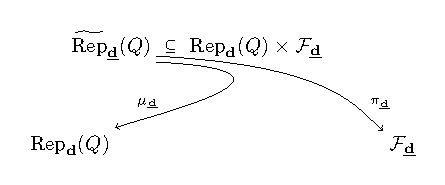
\includegraphics[width=6cm]{figures/comm_diagram/incidence_variety_1.pdf}
			}
			\parbox[t]{.48\textwidth}{\centering
			\vspace{0cm}
			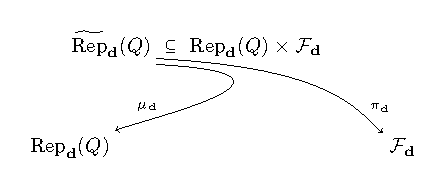
\includegraphics[width=6cm]{figures/comm_diagram/incidence_variety_2.pdf}
			}
			\vspace{-7mm}
	\end{figure}

\begin{remark}\label{rmk:flag_variety_FlagX}
Fix $X \in \Rep_{\dimvec{d}}(Q)$, the flag variety associated to $X$
$$\Flag{\ftdimvec{d}}(X):= \mu_{\ftdimvec{d}}^{-1}(X) \cong \pi_{\ftdimvec{d}}\big(\mu_{\ftdimvec{d}}^{-1}(X)\big) \subseteq \mathcal{F}_{\ftdimvec{d}}$$
records the complete flags of subrepresentations of $X$. The partial flag variety version of $\Flag{\ftdimvec{d}}(X)$ will become the key object in Part \ref{part:partial_flag_varieties}.
\end{remark}
\end{defn}
\begin{defn}[Steinberg variety]
For a quiver $Q$ with complete flag-type dimension vectors $\ftdimvec{d}$, $\ftdimvec{d}'$, define 
\begin{equation*}
\begin{aligned}
  \St_{\ftdimvec{d},\ftdimvec{d}'}:=\;& \RRep_{\ftdimvec{d}}(Q) \times_{\Rep_{\dimvec{d}}(Q)} \RRep_{\ftdimvec{d}'}(Q) \\
  \St_{\dimvec{d}}:=\;& \RRep_{\dimvec{d}}(Q) \times_{\Rep_{\dimvec{d}}(Q)} \RRep_{\dimvec{d}}(Q) \\
  =\;& \bigsqcup_{\ftdimvec{d},\ftdimvec{d}'} \St_{\ftdimvec{d},\ftdimvec{d}'}
\end{aligned}
\end{equation*}
$\St_{\dimvec{d}}$ is called the \textbf{Steinberg variety}.
\end{defn}
$\St_{\ftdimvec{d},\ftdimvec{d}'}$ can actually be realized as the incidence variety between $\Rep_{\dimvec{d}}(Q)$ and $\mathcal{F}_{\ftdimvec{d}} \times \mathcal{F}_{\ftdimvec{d}'}$, since
\begin{equation*}
\begin{aligned}
\St_{\ftdimvec{d},\ftdimvec{d}'}=\;& \RRep_{\ftdimvec{d}}(Q) \times_{\Rep_{\dimvec{d}}(Q)} \RRep_{\ftdimvec{d}'}(Q) \\
\subseteq \;& \left( \Rep_{\dimvec{d}}(Q) \times \mathcal{F}_{\ftdimvec{d}}  \right) 
\times_{\Rep_{\dimvec{d}}(Q)}
\left( \Rep_{\dimvec{d}}(Q) \times \mathcal{F}_{\ftdimvec{d}'}  \right) \\
\cong\;& \Rep_{\dimvec{d}}(Q) \times \mathcal{F}_{\ftdimvec{d}} \times \mathcal{F}_{\ftdimvec{d}'}
\end{aligned}
\end{equation*} 
For that reason, we define $\mu_{\ftdimvec{d},\ftdimvec{d}'}$, $\pi_{\ftdimvec{d},\ftdimvec{d}'}$, $\mu_{\dimvec{d},\dimvec{d}}$, $\pi_{\dimvec{d},\dimvec{d}}$  as natural morphisms from $\St_{\ftdimvec{d},\ftdimvec{d}'}$, $\St_{\dimvec{d}}$ to $\Rep_{\dimvec{d}}(Q)$ or product of flag varieties, as follows:

	\begin{figure}[ht]
		\centering
		\vspace{0cm}
			\parbox[t]{.48\textwidth}{\centering
			\vspace{0cm}
			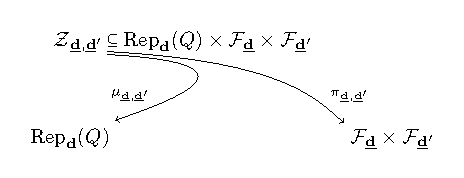
\includegraphics[width=6cm]{figures/comm_diagram/incidence_variety_3.pdf}
			}
			\parbox[t]{.48\textwidth}{\centering
			\vspace{0cm}
			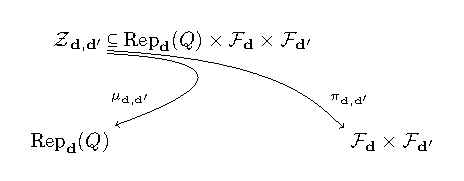
\includegraphics[width=6cm]{figures/comm_diagram/incidence_variety_4.pdf}
			}
	\end{figure}

\begin{remark}[Group actions]\
\begin{enumerate}
\item $\Rep_{\dimvec{d}}(Q)\subseteq \oplus_{r \in a(Q)} \boldsymbol{\mathfrak{g}}_{\abdimvec{d}}$ has a natural $G_{\dimvec{d}}$-action, which is induced by the conjugation action of $G_{\dimvec{d}}$ on $\boldsymbol{\mathfrak{g}}_{\abdimvec{d}}$. We have already mentioned the $G_{\dimvec{d}}$-action on $\mathcal{F}_{\ftdimvec{d}}$ and $\mathcal{F}_{\dimvec{d}}$ in Remark \ref{rmk:action_on_flag}. Therefore, by restriction we automatically get $G_{\dimvec{d}}$-actions on $\RRep_{\ftdimvec{d}}(Q)$, $\RRep_{\dimvec{d}}(Q)$, $\St_{\ftdimvec{d},\ftdimvec{d}'}$ and $\St_{\dimvec{d}}$. All the maps we mentioned in Definition \ref{def:incidence_variety} are $G_{\dimvec{d}}$-equivariant.
\item In Subsection \ref{subsec:Cstar_action} we will also view all the varieties as $G_{\dimvec{d}} \times \mathbb{C}^{\times}$-varieties, so we also shortly introduce $\mathbb{C}^{\times}$-action here. View $\Rep_{\dimvec{d}}(Q)$ as a $\mathbb{C}$-vector space, $\mathbb{C}^{\times}$ acts on $\Rep_{\dimvec{d}}(Q)$ by scalar multiplication. For $\mathcal{F}_{\ftdimvec{d}}$ and $\mathcal{F}_{\dimvec{d}}$, $\mathbb{C}^{\times}$ acts trivially, and by restriction we get $\mathbb{C}^{\times}$-actions on $\RRep_{\ftdimvec{d}}(Q)$, $\RRep_{\dimvec{d}}(Q)$, $\St_{\ftdimvec{d},\ftdimvec{d}'}$ and $\St_{\dimvec{d}}$. Also, all the maps we mentioned above are $\mathbb{C}^{\times}$-equivariant.
\item It may be worth mentioning that $\mathcal{F}_{\dimvec{d}}$ has an $\WWd$-action which can be extended neither to $\absgp{G}_{\abdimvec{d}}$-action on $\mathcal{F}_{\dimvec{d}}$ nor to $\WWd$-action on $\RRep_{\ftdimvec{d}}(Q)$.

\end{enumerate}
\end{remark}


\section{Stratifications and $T$-fixed points}\label{sec:stratification}

%Natural defined varieties resemble burr puzzles, they have delicate structures and can be decomposed into relatively easy pieces. 
In this subsection, we will find stratifications of varieties introduced in Section \ref{sec:typical_variety}, and fix notation of orbits. We will also discuss their $T$-fixed points. These stratifications will give us a basis for the $K$-theory and cohomology in Chapter \ref{chap:Ktheory}, while those $T$-fixed points will give us another ``basis" in Chapter \ref{chap:localization}.

\subsection{Stratifications: flag varieties}
\label{subsec:stratification_flag_variety}
We begin with $\mathcal{F}_{\abdimvec{d}}$ and $\mathcal{F}_{\abdimvec{d}} \times \mathcal{F}_{\abdimvec{d}}$, which is roughly a repetition of Section \ref{sec:inital_case}.

\begin{defn}[Twisted action]
We define the twisted $\absgp{G}_{\abdimvec{d}} \times \absgp{G}_{\abdimvec{d}}$-action on $\mathcal{F}_{\abdimvec{d}} \times \mathcal{F}_{\abdimvec{d}}$:
$$\absgp{G}_{\abdimvec{d}} \times \absgp{G}_{\abdimvec{d}} \times \mathcal{F}_{\abdimvec{d}} \times \mathcal{F}_{\abdimvec{d}} \longrightarrow \mathcal{F}_{\abdimvec{d}} \times \mathcal{F}_{\abdimvec{d}} \qquad \left( g_1,g_2,\underline{F}_{g,g'} \right) \longmapsto \underline{F}_{g_1g,g_2g'}$$
which is the same as original $\absgp{G}_{\abdimvec{d}}$-action when we restrict to $\absgp{G}_{\abdimvec{d}} \times \{\Id \}$-action. Other $G \times G$-actions on $\mathcal{F} \times \mathcal{F}$ are defined in a similar way.
\end{defn}

\begin{defn}[Stratifications of $\mathcal{F}_{\abdimvec{d}}$ and $\mathcal{F}_{\abdimvec{d}} \times \mathcal{F}_{\abdimvec{d}}$]
For $\ww,\ww' \in \WWd$, we define
\begin{equation*}
\begin{aligned}
  \Vcell_{\ww}=\;& \absgp{B}_{\abdimvec{d}} \cdot F_{\ww} \qquad&& \subseteq \mathcal{F}_{\abdimvec{d}} \\ 
  \VVcell_{\ww,\ww'}=\;& \left(\absgp{B}_{\abdimvec{d}} \times \absgp{B}_{\abdimvec{d}}\right) \cdot \underline{F}_{\ww,\ww'} && \subseteq \mathcal{F}_{\abdimvec{d}} \times \mathcal{F}_{\abdimvec{d}} \\ 
  \VVcell_{\ww'}=\;& \absgp{G}_{\abdimvec{d}} \cdot \underline{F}_{\Id,\ww'} && \subseteq \mathcal{F}_{\abdimvec{d}} \times \mathcal{F}_{\abdimvec{d}} \\ 
\end{aligned}
\end{equation*}
as $\absgp{B}_{\abdimvec{d}}$-orbit, $\absgp{B}_{\abdimvec{d}} \times \absgp{B}_{\abdimvec{d}}$-orbit, $\absgp{G}_{\abdimvec{d}}$-orbit of $\mathcal{F}_{\abdimvec{d}}$, $\mathcal{F}_{\abdimvec{d}} \times \mathcal{F}_{\abdimvec{d}}$ and  $\mathcal{F}_{\abdimvec{d}} \times \mathcal{F}_{\abdimvec{d}}$, respectively.
\end{defn}

By Bruhat-decomposition, we are able to show
$$\mathcal{F}_{\abdimvec{d}}= \bigsqcup_{\ww} \Vcell_{\ww} \qquad \mathcal{F}_{\abdimvec{d}} \times \mathcal{F}_{\abdimvec{d}} = \bigsqcup_{\ww'} \VVcell_{\ww'} = \bigsqcup_{\ww,\ww'} \VVcell_{\ww,\ww'}.$$
We also realize these orbits as quotients of algebraic groups by the orbit-stabilizer theorem, as follows:
\begin{equation*}
\begin{aligned}
  \Vcell_{\ww}\cong\;& \absgp{B}_{\abdimvec{d}} /\left(  \absgp{B}_{\abdimvec{d}} \cap \absgp{B}_{\ww} \right) \qquad&&  \cong \mathbb{A}^{l(\ww)} \\ 
  \VVcell_{\ww,\ww'}\cong\;& \left(\absgp{B}_{\abdimvec{d}} \times \absgp{B}_{\abdimvec{d}}\right) / \left(\absgp{B}_{\abdimvec{d}} \cap \absgp{B}_{\ww} \times \absgp{B}_{\abdimvec{d}} \cap \absgp{B}_{\ww'}\right)&& \cong \mathbb{A}^{l(\ww)+l(\ww')}  \\ 
  \VVcell_{\ww'}\cong\;& \absgp{G}_{\abdimvec{d}} /\left(  \absgp{B}_{\abdimvec{d}} \cap \absgp{B}_{\ww'} \right) && \cong \mathbb{A}^{l(\ww')}\text{-bundle over }\mathcal{F}_{\abdimvec{d}}  \\ 
\end{aligned}
\end{equation*}

Similar stratifications happen for $\mathcal{F}_{u}$ and $\mathcal{F}_{\dimvec{d}}$.

\begin{defn}[Stratifications of $\mathcal{F}_{u}$ and $\mathcal{F}_{u} \times \mathcal{F}_{u'}$]
For $u,u' \in \MinWd$, $w,w' \in \Wd$, we define
\begin{equation*}
\begin{aligned}
  \Omcell_{w}^{u}=\;& B_{\dimvec{d}} \cdot F_{wu} \qquad&& \subseteq \mathcal{F}_{u} \\ 
  \OOmcell_{w,w'}^{u,u'}=\;& \left(B_{\dimvec{d}} \times B_{\dimvec{d}}\right) \cdot \left( F_{wu}, F_{ww'u'} \right)  && \subseteq \mathcal{F}_{u} \times \mathcal{F}_{u'}\\ 
  \OOmcell_{w'}^{u,u'}=\;&  G_{\dimvec{d}} \cdot \left( F_{u}, F_{w'u'} \right) && \subseteq \mathcal{F}_{u} \times \mathcal{F}_{u'} \\ 
\end{aligned}
\end{equation*}
as $B_{\dimvec{d}}$-orbit, $B_{\dimvec{d}} \times B_{\dimvec{d}}$-orbit, $G_{\dimvec{d}}$-orbit of $\mathcal{F}_{u}$, $\mathcal{F}_{u} \times \mathcal{F}_{u'}$ and $\mathcal{F}_{u} \times \mathcal{F}_{u'}$, respectively.
\end{defn}

By Bruhat decomposition, we are again able to show
$$\mathcal{F}_{u}= \bigsqcup_{w} \Omcell_{w}^{u} \qquad \mathcal{F}_{u} \times \mathcal{F}_{u'} = \bigsqcup_{w'} \OOmcell_{w'}^{u,u'} = \bigsqcup_{w,w'} \OOmcell_{w,w'}^{u,u'}$$
and
\begin{equation*}
\begin{aligned}
  \Omcell_{w}^{u}\cong\;& B_{\dimvec{d}} /\left(  B_{\dimvec{d}} \cap B_{w} \right) \qquad&&  \cong \mathbb{A}^{l(w)} \\ 
  \OOmcell_{w,w'}^{u,u'}\cong\;& \left(B_{\dimvec{d}} \times B_{\dimvec{d}}\right) / \left(B_{\dimvec{d}} \cap B_{w} \times B_{\dimvec{d}} \cap B_{w'}\right)&& \cong \mathbb{A}^{l(w)+l(w')}  \\ 
  \OOmcell_{w'}^{u,u'}\cong\;& G_{\dimvec{d}} /\left(  B_{\dimvec{d}} \cap B_{w'} \right) && \cong \mathbb{A}^{l(w')}\text{-bundle over }\mathcal{F}_{u}  \\ 
\end{aligned}
\end{equation*}

\begin{defn}[Stratifications of $\mathcal{F}_{\dimvec{d}}$ and $\mathcal{F}_{\dimvec{d}} \times \mathcal{F}_{\dimvec{d}}$]
For $\ww,\ww' \in \WWd$, we define
\begin{equation*}
\begin{aligned}
  \Ocell_{\ww}=\;& B_{\dimvec{d}} \cdot F_{\ww} \qquad&&\subseteq \mathcal{F}_{\ww}&& \subseteq \mathcal{F}_{\dimvec{d}} \\ 
  \OOcell_{\ww,\ww'}=\;& \left(B_{\dimvec{d}} \times B_{\dimvec{d}}\right) \cdot \underline{F}_{\ww,\ww'} && \subseteq \mathcal{F}_{\ww} \times \mathcal{F}_{\ww\ww'} && \subseteq \mathcal{F}_{\dimvec{d}} \times \mathcal{F}_{\dimvec{d}}\\ 
  \OOcell_{\ww'}=\;& \bigsqcup_{u} G_{\dimvec{d}} \cdot \underline{F}_{u,\ww'} && \subseteq \bigsqcup_{u}\mathcal{F}_{u} \times \mathcal{F}_{u\ww'}\hspace{-1cm}&& \subseteq \mathcal{F}_{\dimvec{d}} \times \mathcal{F}_{\dimvec{d}} \\ 
\end{aligned}
\end{equation*}
as $B_{\dimvec{d}}$-orbit, $B_{\dimvec{d}} \times B_{\dimvec{d}}$-orbit, (union of) $G_{\dimvec{d}}$-orbit of $\mathcal{F}_{\dimvec{d}}$, $\mathcal{F}_{\dimvec{d}} \times \mathcal{F}_{\dimvec{d}}$ and $\mathcal{F}_{\dimvec{d}} \times \mathcal{F}_{\dimvec{d}}$, respectively.
\end{defn}
Notice that $\Ocell_{\ww}$, $\OOcell_{\ww,\ww'}$, $\OOcell_{\ww'}$ are preimages of $\Vcell_{\ww}$, $\VVcell_{\ww,\ww'}$, $\VVcell_{\ww'}$ under the maps
$$\mathcal{F}_{\dimvec{d}} \hookrightarrow  \mathcal{F}_{\abdimvec{d}} \qquad \mathcal{F}_{\dimvec{d}} \times \mathcal{F}_{\dimvec{d}} \hookrightarrow  \mathcal{F}_{\abdimvec{d}} \times \mathcal{F}_{\abdimvec{d}}.$$
Therefore, 
$$\mathcal{F}_{\dimvec{d}}= \bigsqcup_{\ww} \Ocell_{\ww} \qquad \mathcal{F}_{\dimvec{d}} \times \mathcal{F}_{\dimvec{d}} = \bigsqcup_{\ww'} \OOcell_{\ww'} = \bigsqcup_{\ww,\ww'} \OOcell_{\ww,\ww'}.$$

%Some stratifications are quite compatible with the connected component of $\mathcal{F}_{\dimvec{d}}$, so we give new names for them.



We still need to care about symbols. For $\ww=wu$, $\ww'=w'u'$, denote $uw'u'$ by $\tilde{w}\tilde{u}$ for some unique $\tilde{w} \in \Wd$, $\tilde{u} \in \MinWd$, then
$$\underline{F}_{\ww,\ww'}= \left( F_{\ww}, F_{\ww\ww'}  \right)= \left( F_{wu}, F_{wuw'u'}  \right)= \left( F_{wu}, F_{w\tilde{w}\tilde{u}}  \right) \in \mathcal{F}_{u} \times \mathcal{F}_{\tilde{u}}.$$
This incompatibility comes from our twisted $G_{\dimvec{d}} \times G_{\dimvec{d}}$-actions. In particular, denote
$$\OOcell_{\ww'}^{u}:= G_{\dimvec{d}} \cdot \underline{F}_{u,\ww'}\subseteq \mathcal{F}_{u} \times \mathcal{F}_{\tilde{u}},$$
we have $\OOcell_{\ww'}=\sqcup_{u} \OOcell_{\ww'}^{u}$ and identifications
\begin{equation}\label{eq:identification}
\Ocell_{\ww}=\Omcell_{w}^{u} \qquad \OOcell_{\ww,\ww'}=\OOmcell_{w,\tilde{w}}^{u,\tilde{u}} \qquad \OOcell_{\ww'}^{u}=\OOmcell_{\tilde{w}}^{u,\tilde{u}}.
\end{equation}
 \begin{table}
   \vspace{0cm}
     \centering  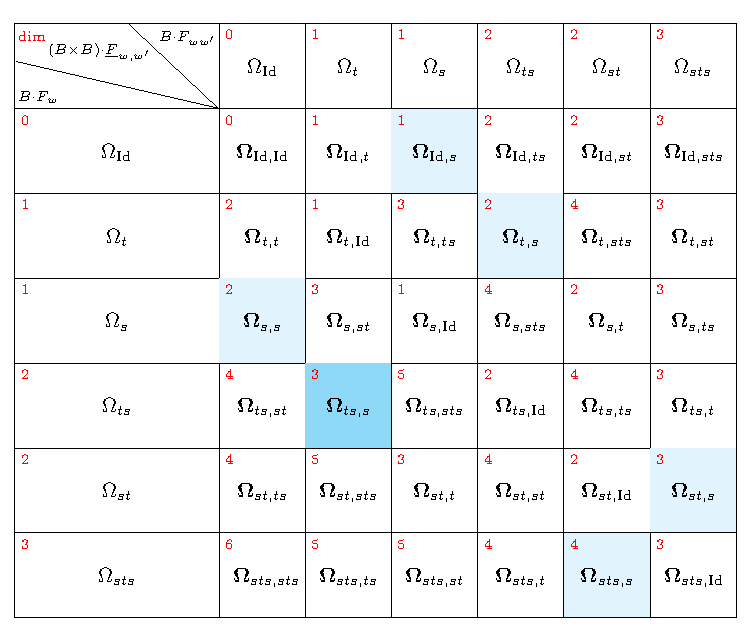
\includegraphics[width=12.5cm]{figures/table/table_1.pdf}
         \caption{stratifications of $\mathcal{F}\times \mathcal{F}$}
         \label{table:stratifications_of_FF}
  \vspace{1cm} 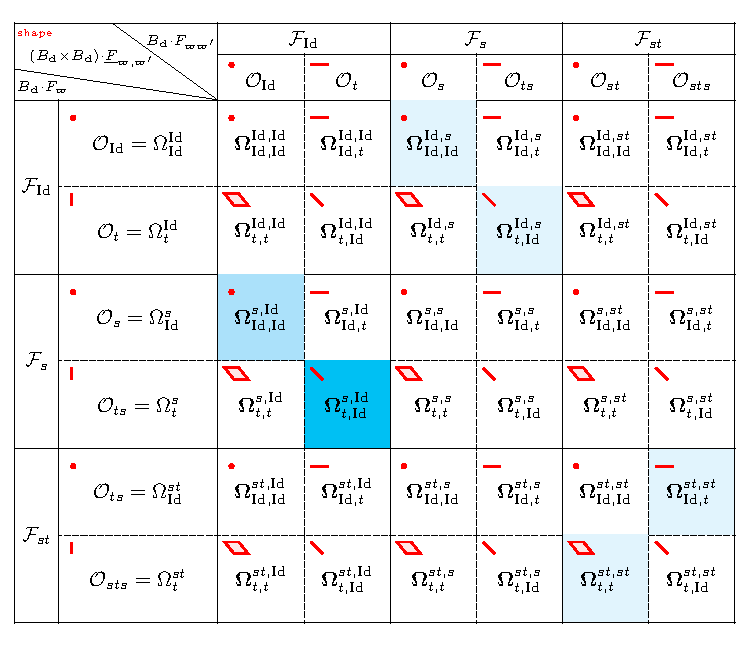
\includegraphics[width=12.5cm]{figures/table/table_2.pdf}
        \caption{stratifications of $\mathcal{F}_{\dimvec{d}}\times \mathcal{F}_{\dimvec{d}}$}
        \label{table:stratifications_of_FdFd}
\end{table}

After so much notation is introduced rapidly, an enlightening example is needed here.
\begin{eg}[Follows Example \ref{eg:3-case-1}]\label{eg:3-case-2}
In Table \ref{table:stratifications_of_FdFd}, $\WWd=S_3$, $\Wd=S_1 \times S_2$,
$$\ww=ts=t \cdot s, \qquad \ww'=s=\Id \cdot s,\qquad \ww\ww'=t=t \cdot \Id.$$

$\mathcal{F}_{\dimvec{d}}$ has $3$ connected components, each of them has $2$ $B_{\dimvec{d}}$-orbits;

 $\mathcal{F}_{\dimvec{d}} \times \mathcal{F}_{\dimvec{d}}$ has $9$ connected components, each of them has $4$ $B_{\dimvec{d}} \times B_{\dimvec{d}}$-orbits.

We have given every orbit a name, and other spaces are finite union of these orbits. For example,
\begin{equation*}
\begin{aligned}
  \OOcell_{ts,s}=\;& \OOmcell_{t,\Id}^{s,\Id} \\ 
  \OOcell_{s}^{s}=\;& \OOmcell_{\Id}^{s,\Id} = \OOmcell_{\Id,\Id}^{s,\Id} \sqcup \OOmcell_{t,\Id}^{s,\Id} \\ 
  \OOcell_{s}=\;& \OOcell_{s}^{s} \sqcup \OOcell_{s}^{\Id} \sqcup \OOcell_{s}^{st} \\   
  =\;& \OOcell_{s}^{s} \sqcup \OOcell_{s}^{\Id} \sqcup \OOcell_{s}^{st} \\  
  =\;& \OOmcell_{\Id}^{s,\Id} \sqcup \OOmcell_{\Id}^{\Id,s} \sqcup \OOmcell_{\Id}^{st,st}
   \\  
  =\;& \OOmcell_{\Id,\Id}^{s,\Id} \sqcup \OOmcell_{t,\Id}^{s,\Id} \sqcup \OOmcell_{\Id,\Id}^{\Id,s} \sqcup  \OOmcell_{t,\Id}^{\Id,s} \sqcup \OOmcell_{\Id,\Id}^{st,st} \sqcup \OOmcell_{t,\Id}^{st,st}
   \\  
\end{aligned}
\end{equation*}
%Their closures are also clear from the table, for example, 
%$$\overline{\OOcell}_s=\OOcell_{s} \sqcup \OOmcell_{\Id}^{st,st}$$
%contains $8$ $B_{\dimvec{d}} \times B_{\dimvec{d}}$-orbits.
\end{eg}


\subsection{Stratifications: incidence varieties}\label{subsec:stratification:_incidence_variety}
Now comes the stratifications of incidence varieties. Those stratifications are produced by taking the preimage of stratifications on base spaces. They are relatively easy to obtain, while their closures are quite difficult to analyze.

\begin{defn}[Stratifications of incidence varieties]
For $\ww=wu$, $\ww'=w'u' \in \WWd$, denote $\tilde{w}\tilde{u}=uwu' $, $\ftdimvec{d}=\Wd u$, $\ftdimvec{d}'=\Wd u'$, $\widetilde{\ftdimvec{d}}=\Wd \tilde{u}$. We define

\begin{align*}
  \preimage{\Omcell}_{w}^{u}:=\;& \pi_{\ftdimvec{d}}^{-1}(\Omcell_{w}^{u})&& \subseteq \RRep_{\ftdimvec{d}}(Q) &\preimage{\Ocell}_{\ww}:=\;& \pi_{\dimvec{d}}^{-1}(\Ocell_{\ww})\hspace{-7mm}&& \subseteq \RRep_{\dimvec{d}}(Q)\\ 
  \preimage{\OOmcell}_{w,w'}^{u,u'}:=\;& \pi_{\ftdimvec{d},\ftdimvec{d}'}^{-1}(\OOmcell_{w,w'}^{u,u'})&& \subseteq \St_{\ftdimvec{d},\ftdimvec{d}'} &\preimage{\OOcell}_{\ww,\ww'}:=\;& \pi_{\dimvec{d},\dimvec{d}'}^{-1}(\OOcell_{\ww,\ww'})\hspace{-7mm}&& \subseteq \St_{\dimvec{d}} \\ 
  \preimage{\OOmcell}_{w'}^{u,u'}:=\;& \pi_{\ftdimvec{d},\ftdimvec{d}'}^{-1}(\OOmcell_{w'}^{u,u'})&& \subseteq \St_{\ftdimvec{d},\ftdimvec{d}'} &\preimage{\OOcell}_{\ww'}:=\;& \pi_{\dimvec{d},\dimvec{d}'}^{-1}(\OOcell_{\ww'})\hspace{-7mm}&& \subseteq \St_{\dimvec{d}} \\ 
  \preimage{\OOcell}_{\ww'}^{u}:=\;& \pi_{\ftdimvec{d},\widetilde{\ftdimvec{d}}}^{-1}(\OOcell_{\ww'}^{u}) = \preimage{\OOmcell}_{\tilde{w}}^{u,\tilde{u}}\hspace{-7mm}&& \subseteq \St_{\ftdimvec{d},\widetilde{\ftdimvec{d}}} \\
\end{align*}
\end{defn}


It is not hard to see that they are stratifications:
\begin{equation*}
\begin{aligned}
  \RRep_{\ftdimvec{d}}(Q)=\;& \bigsqcup_{\ww} \preimage{\Omcell}_{w}^{u} \qquad &  \St_{\ftdimvec{d},\ftdimvec{d}'} =\;& \bigsqcup_{w} \preimage{\OOmcell}_{w'}^{u,u'} = \bigsqcup_{w,w'} \preimage{\OOmcell}_{w,w'}^{u,u'}  \\
  \RRep_{\dimvec{d}}(Q)=\;& \bigsqcup_{\ww} \preimage{\Ocell}_{\ww} \qquad &  \St_{\dimvec{d}} =\;& \bigsqcup_{\ww'} \preimage{\OOcell}_{\ww'} = \bigsqcup_{\ww,\ww'} \preimage{\OOcell}_{\ww,\ww'}  \\
\end{aligned}
\end{equation*}

\begin{proposition}\label{prop:strataffine}
Those stratifications are affine spaces over corresponding base spaces. To be precise,
\begin{equation*}
\begin{aligned}
  \preimage{\Omcell}_{w}^{u}=\;& \mathfrak{r}_{wu}\text{-bundle over }\Omcell_{w}^{u}  \quad&\preimage{\Ocell}_{\ww}=\;&\mathfrak{r}_{\ww}\text{-bundle over }\Ocell_{\ww} \\ 
  \preimage{\OOmcell}_{w,w'}^{u,u'}=\;&\mathfrak{r}_{wu,ww'u'}\text{-bundle over }\OOmcell_{w,w'}^{u,u'} \quad&\preimage{\OOcell}_{\ww,\ww'}=\;&\underline{\mathfrak{r}}_{\ww,\ww'}\text{-bundle over }\OOcell_{\ww,\ww'} \\ 
  \preimage{\OOmcell}_{w'}^{u,u'}=\;&\mathfrak{r}_{u,w'u'}\text{-bundle over }\OOmcell_{w'}^{u,u'}\quad&\preimage{\OOcell}_{\ww'}=\;&\underline{\mathfrak{r}}_{\Id,\ww'}\text{-bundle over }\OOcell_{\ww'} \\ 
  \preimage{\OOcell}_{\ww'}^{u}=\;&\underline{\mathfrak{r}}_{u,\ww'}\text{-bundle over }\OOcell_{\ww'}^{u} 
\end{aligned}
\end{equation*}
\end{proposition}

\begin{proof}
The fibers are all computed over the preferred base point. The group action induces the isomorphism between different fibers, and lift affine local charts on base space (viewed as group quotient) to the local charts of fiber bundles. 
\end{proof}

We end this subsection by Table \ref{table:orbit}:
\begin{table}[ht]
  \vspace{0cm}
    \centering  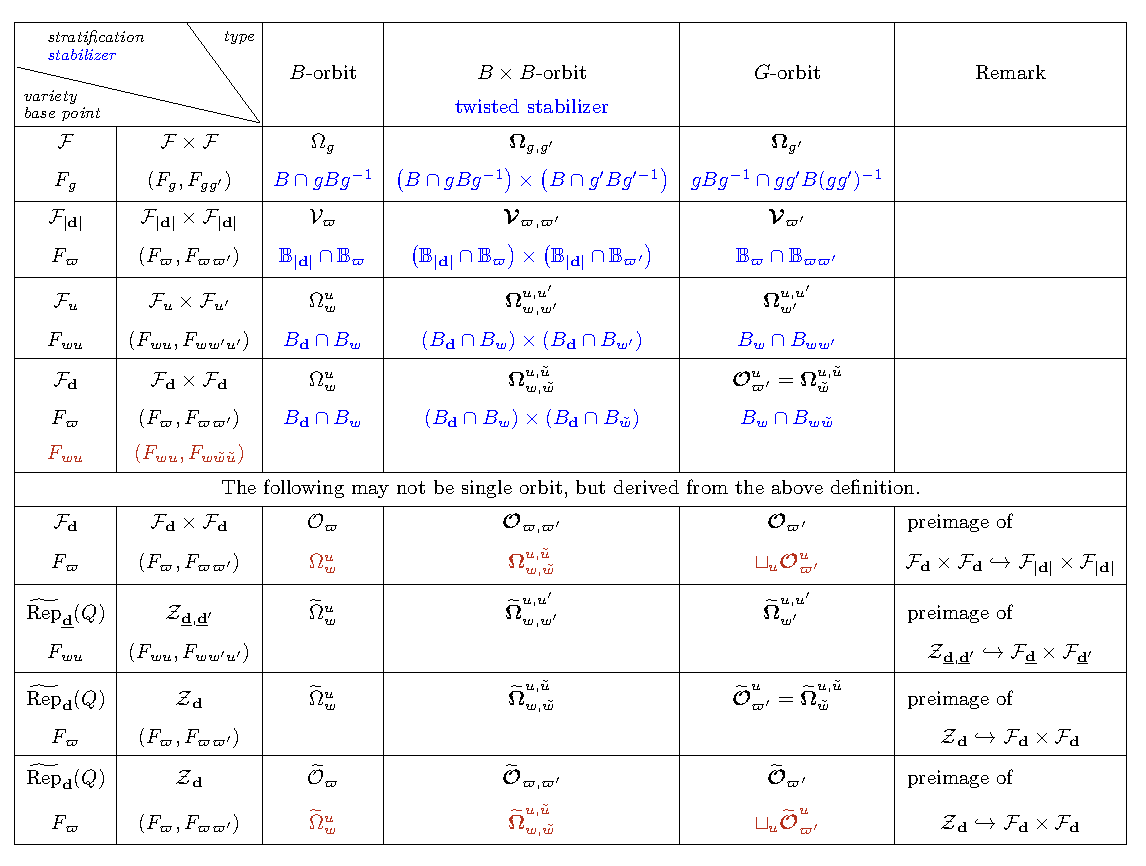
\includegraphics[width=15cm]{figures/table/table_orbit.pdf}
      \caption{stratifications of typical varieties}
      \label{table:orbit}    
      \vspace{3mm}    
\end{table}
\subsection{Closure of cells}

In this subsection we describe the closure of cells. We begin with $\OOmcell$-cells:
\begin{equation*}
  \overline{\Omcell}_{w}^{u}= \bigsqcup_{x\leqslant w}\Omcell_{x}^{u}  \qquad
  \overline{\OOmcell}_{w,w'}^{u,u'}=\bigsqcup_{x \leqslant w, x'\leqslant w'} \OOmcell_{x,x'}^{u,u'} \qquad
  \overline{\OOmcell}_{w'}^{u,u'}=\bigsqcup_{x'\leqslant w'} \OOmcell_{x'}^{u,u'} \\ 
\end{equation*}
Especially, for any $s \in \Pi_{\dimvec{d}}$, $u,u' \in \MinWd$, we have
$$\overline{\OOmcell}_{s}^{u,u'} = \OOmcell_{s}^{u,u'} \sqcup \OOmcell_{\Id}^{u,u'} \cong G_{\dimvec{d}} \times^{B_{\dimvec{d}}} \left( P_{\Id,s} / B_{\dimvec{d}} \right)$$
when we work over base point $F_{u,u'}$. If we work over different base points, we will get different isomorphisms, as follows:
\begin{equation*}
\begin{aligned}
 \overline{\OOmcell}_{s}^{u,u'} = \OOmcell_{\Id}^{u,u'}\sqcup \OOmcell_{s}^{u,u'} \cong\;& 
  G_{\dimvec{d}} /(B_w \cap B_{ws} ) &&\sqcup G_{\dimvec{d}}/B_w \\ 
  \cong\;&  G_{\dimvec{d}} \times^{B_w} \big(B_w/(B_w \cap B_{ws})\big)\hspace{-0.4cm} &&\sqcup G_{\dimvec{d}} \times^{B_w} (B_w/B_w) \\ 
  \cong\;& G_{\dimvec{d}} \times^{B_w} (B_w sB_w/B_w) &&\sqcup G_{\dimvec{d}} \times^{B_w} (B_w/B_w)  \\ 
  \cong\;& G_{\dimvec{d}} \times^{B_w} (\underline{P}_{w,s}/B_w)&& \qquad \text{ base point }F_{wu,wu'}\\ 
  \cong\;& G_{\dimvec{d}} \times^{B_w} (\underline{P}_{w,s}/B_{ws})&& \qquad \text{ base point }F_{wu,wsu'}\\ 
\end{aligned}
\end{equation*}

Closures of $\OOcell$-cells are obtained by identifications \eqref{eq:identification}. To illustrate it, we compute $\overline{\OOcell}_s$ by hand. Let $\ww'=s, us=\tilde{w}\tilde{u}$,
 
\begin{align*}
 \overline{\OOcell}_{s} = \;&\bigsqcup_u \overline{\OOcell}_{s}^{u} = \bigsqcup_u \overline{\OOmcell}_{\tilde{w}}^{u,\tilde{u}}\\
 =\;& \left(\raisebox{1.4mm}{$\displaystyle\bigsqcup_{u:usu^{-1} \in \Wd}$} \overline{\OOmcell}_{usu^{-1}}^{u,u}\right) \sqcup \left(\raisebox{1.4mm}{$\displaystyle\bigsqcup_{u:usu^{-1} \notin \Wd}$} \overline{\OOmcell}_{\Id}^{u,us}\right)\\
 =\;& \left(\raisebox{1.4mm}{$\displaystyle\bigsqcup_{u:usu^{-1} \in \Wd}$} \OOmcell_{usu^{-1}}^{u,u}\right) \sqcup \left(\raisebox{1.4mm}{$\displaystyle\bigsqcup_{u:usu^{-1} \notin \Wd}$} \OOmcell_{\Id}^{u,us}\right) \sqcup \left(\raisebox{1.4mm}{$\displaystyle\bigsqcup_{u:usu^{-1} \in \Wd}$} \OOmcell_{\Id}^{u,u}\right)\\
 =\;&\OOcell_{s} \sqcup \left(\raisebox{1.4mm}{$\displaystyle\bigsqcup_{u:usu^{-1} \in \Wd}$} \OOcell_{\Id}^{u}\right)
\end{align*}

We restrict the result of $\overline{\OOmcell}_{s}^{u,u'}$ to $\overline{\OOcell}_{s}^{u}$ in Lemma \ref{lem:iso_of_orbits}.

\begin{lemma}\label{lem:iso_of_orbits}
For $\ww=wu \in \WWd$, $s\in \Pi$ such that $\ww s \ww^{-1} \in \Wd$, we have isomorphisms of $G_{\dimvec{d}}$-varieties
\begin{equation*}
\begin{aligned}
& G_{\dimvec{d}} \times^{B_{\ww}} (\underline{P}_{\ww,s}/B_{\ww}) \longrightarrow \overline{\OOcell}_{s}^{u} \qquad && (g,p) \longmapsto (g \cdot F_{\ww}, gp \cdot F_{\ww})\\
& G_{\dimvec{d}} \times^{B_{\ww}} (\underline{P}_{\ww,s}/B_{\ww s}) \longrightarrow \overline{\OOcell}_{s}^{u} \qquad && (g,p) \longmapsto (g \cdot F_{\ww}, gp \cdot F_{\ww s})\\
\end{aligned}
\end{equation*}
\end{lemma}
\begin{proof}
Notice that when $\ww s \ww^{-1} \in \Wd$, $\OOcell_{s}^{u}=\OOmcell_{usu^{-1}}^{u,u}$. Therefore, 
\begin{equation*}
\begin{aligned}
 \overline{\OOcell}_{s}^{u}=\overline{\OOmcell}_{usu^{-1}}^{u,u} \cong\;& 
 \begin{cases}
 G_{\dimvec{d}} \times^{B_w} (\underline{P}_{w,usu^{-1}}/B_w) & \text{ base point }F_{wu,wu} \\
 G_{\dimvec{d}} \times^{B_w} (\underline{P}_{w,usu^{-1}}/B_{wusu^{-1}}) & \text{ base point }F_{wu,wus} 
 \end{cases} \\ 
  \cong\;& 
  \begin{cases}
  G_{\dimvec{d}} \times^{B_{\ww}} (\underline{P}_{\ww,s}/B_{\ww}) & \qquad\text{ base point }F_{\ww,\ww} \\
  G_{\dimvec{d}} \times^{B_{\ww}} (\underline{P}_{\ww,s}/B_{\ww s}) & \qquad\text{ base point }F_{\ww,\ww s} 
  \end{cases} \\ 
\end{aligned}
\end{equation*}
\\[-2\baselineskip]
\end{proof}


\begin{defn}
We define
\begin{equation*}
\begin{aligned}
  \St_{w'}^{u,u'}:=\;& \overline{\preimage{\OOmcell}}_{w'}^{u,u'} && \subseteq \hspace{7mm}\St^{u,u'}:= \St_{\ftdimvec{d},\ftdimvec{d}'}, \\
  \St_{\ww'}:=\;& \overline{\preimage{\OOcell}}_{\ww'} && \subseteq \phantom{\hspace{7mm} \St^{u,u'}:=}\St_{\dimvec{d}}.
\end{aligned}
\end{equation*}
\end{defn}

%\begin{proposition}[Properties of the closure]
%$\St_{\ww'}$ is a Zarisky-locally trivial cone bundle over $\mathcal{F}_{\dimvec{d}} \times \mathcal{F}_{\dimvec{d}}$. To be precise, under the map
%$$\pi_{\dimvec{d},\dimvec{d},\ww'}: \St_{\ww'} \longrightarrow \mathcal{F}_{\dimvec{d}} \times \mathcal{F}_{\dimvec{d}},$$
%for any $x,x' \in \WWd$, $\pi_{\dimvec{d},\dimvec{d},\ww'}^{-1}(\OOcell_{x,x'})$ is a trivial fiber bundle over $\OOcell_{x,x'}$, whose fibers are cones.
%\end{proposition}
%
%Notice that
%\begin{equation*}
%\begin{aligned}
%  \St_{w'}^{u,u'}:=\;& \overline{\preimage{\OOmcell}}_{w'}^{u,u'} && \subseteq \hspace{7mm}\preimage{\overline{\OOmcell}}_{w'}^{u,u'}:= \pi_{\ftdimvec{d},\ftdimvec{d}'}^{-1}\left( \overline{\OOmcell}_{w'}^{u,u'} \right), \\
%  \St_{\ww'}:=\;& \overline{\preimage{\OOcell}}_{\ww'} && \subseteq \hspace{7mm} \preimage{\overline{\OOcell}}_{\ww'} :=\pi_{\dimvec{d},\dimvec{d}}^{-1}\left( \overline{\OOcell}_{\ww'} \right).
%\end{aligned}
%\end{equation*}
%Even though these inclusions are usually not equalities, we can still say something when the length of $w'$ or $\ww'$ is small. For example,
%\begin{equation*}
%\begin{aligned}
%&\St_{\Id}^{u,u'}=\preimage{\OOmcell}_{\Id}^{u,u'} \\ 
%&\St_{\Id}=\preimage{\OOcell}_{\Id}\\
%\preimage{\OOmcell}_{s}^{u,u'}\sqcup \OOmcell_{\Id}^{u,u'} \subseteq &\St_{s}^{u,u'} \subseteq \preimage{\OOmcell}_{s}^{u,u'}\sqcup \preimage{\OOmcell}_{\Id}^{u,u'} \qquad &(s \in \Pi_{\dimvec{d}})\\
% \preimage{\OOcell}_{s} \sqcup \left(\bigsqcup_{u:usu^{-1} \in \Wd}\OOcell_{\Id}^{u}\right) \subseteq& \St_{s} \subseteq \preimage{\OOcell}_{s} \sqcup \left(\bigsqcup_{u:usu^{-1} \in \Wd}\preimage{\OOcell}_{\Id}^{u}\right) \qquad &(s \in \Pi_{\phantom{d}})
%\end{aligned}
%\end{equation*}

\begin{proposition}\label{prop:vector_bundle_Z_s}
$\St_s$ is a Zarisky-locally trivial vector bundle over $\overline{\OOcell}_s$, with fiber $\mathfrak{r}_{u,us}$ at point $\underline{F}_{u,s}$.
\end{proposition}
\begin{proof}
This is claimed in \cite[2.20(c)]{varagnolo2011canonical}. In fact, we have a $G_{\dimvec{d}}$-equivariant morphism
$$\phi: G_{\dimvec{d}} \times^{B_u} \left(  \underline{P}_{u,s}/B_{us} \times \underline{\mathfrak{r}}_{u,s} \right) \hookrightarrow \Rep_{\dimvec{d}}(Q) \times \mathcal{F}_{\dimvec{d}} \times \mathcal{F}_{\dimvec{d}} \qquad (g,p,x) \longmapsto (gx, g \cdot F_u, gp \cdot F_{us})$$
which realized $G_{\dimvec{d}} \times^{B_u} \left(  \underline{P}_{u,s}/B_{us} \times \underline{\mathfrak{r}}_{u,s} \right)$ as a closed subset of $\Rep_{\dimvec{d}}(Q) \times \mathcal{F}_{\dimvec{d}}$. In the meantime, the open dense subset $$G_{\dimvec{d}} \times^{B_u} \left(  B_{us}sB_{us}/B_{us}\times \underline{\mathfrak{r}}_{u,s} \right) \subseteq G_{\dimvec{d}} \times^{B_u} \left(  \underline{P}_{u,s}/B_{us}\times \underline{\mathfrak{r}}_{u,s} \right)$$
 is identified with $\preimage{\OOcell}_{s}^{u}$ by $\phi$. Therefore, $\phi$ identifies $\St_{s}^{u,\tilde{u}}$ with the vector bundle $G_{\dimvec{d}} \times^{B_u} \left(  \underline{P}_{u,s}/B_{us} \times \underline{\mathfrak{r}}_{u,s} \right)$ over $\overline{\OOcell}_{s}^{u}$, with fiber $\underline{\mathfrak{r}}_{u,s}=\mathfrak{r}_{u,us}$.
\end{proof}

\begin{remark}\label{rmk:vector_bundle_O_s}
By the same method, one can show that $\overline{\preimage{\Ocell}}_{s}$ is a Zarisky-locally trivial vector bundle over $\overline{\Ocell}_s$, with fiber $\mathfrak{r}_{s}$ at point $F_{s}$.
\end{remark}

\subsection{$T$-fixed points}

Recall that the $T$-fixed points of a complete flag variety $\mathcal{F}$ are exactly the coordinate flags $\left\{ F_w \,\middle|\, w \in W \right\}$. For absolute or relative flag varieties, we have similar results:
$$\mathcal{F}_{\abdimvec{d}}^{\absgp{T}_{\abdimvec{d}}} = \mathcal{F}_{\dimvec{d}}^{T_{\dimvec{d}}}= \left\{ F_{\ww} \,\middle|\, \ww \in \WWd \right\} \qquad \mathcal{F}_u^{T_{\dimvec{d}}} = \left\{ F_{wu} \,\middle|\, w \in \Wd \right\}$$ 
For $\Rep_{\dimvec{d}}(Q)$, we get
$$\big(\!\Rep_{\dimvec{d}}(Q) \big)^{T_{\dimvec{d}}} = \bigoplus_{r \in a(Q)} \bigg( \Hom \left(\mathbb{C}^{\dimvec{d}_{s(a)}},\mathbb{C}^{\dimvec{d}_{t(a)}}\right) \bigg)^{T_{\dimvec{d}}} =\{ \rho_0 \}$$
where $\rho_0$ is the zero representation in $\Rep_{\dimvec{d}}(Q)$.

Combining these two results, one can easily describe $T$-fixed points of varieties constructed over them:
\begin{align*}
  \left(\mathcal{F}_{\abdimvec{d}} \times \mathcal{F}_{\abdimvec{d}}\right)^{\absgp{T}_{\abdimvec{d}}}=\;& \left\{  (F_{\ww},F_{\ww'}) \,\middle|\,  \ww,\ww' \in \WWd  \right\}\quad& \left(\RRep_{\ftdimvec{d}}(Q)\right)^{T_{\dimvec{d}}}=\;& \left\{  (\rho_0,F_{wu}) \,\middle|\,  w \in \Wd  \right\}\\ 
  \left(\mathcal{F}_{u} \times \mathcal{F}_{u'}\right)^{T_{\dimvec{d}}}=\;&  \left\{  (F_{wu},F_{w'u'}) \,\middle|\,  w,w' \in \Wd  \right\} \quad&\left(\RRep_{\dimvec{d}}(Q)\right)^{T_{\dimvec{d}}}=\;& \left\{  (\rho_0,F_{\ww}) \,\middle|\,  \ww \in \WWd  \right\} \\ 
  \left(\mathcal{F}_{\dimvec{d}} \times \mathcal{F}_{\dimvec{d}}\right)^{T_{\dimvec{d}}}=\;&  \left\{  (F_{\ww},F_{\ww'}) \,\middle|\,  \ww,\ww' \in \WWd  \right\} \quad&\left(\St_{\ftdimvec{d},\ftdimvec{d}'}\right)^{T_{\dimvec{d}}}=\;&  \left\{  (\rho_0,F_{wu},F_{w'u'}) \,\middle|\,  w,w' \in \Wd  \right\}\\[2mm]
  &\quad&\left(\St_{\dimvec{d}}\right)^{T_{\dimvec{d}}}=\;& \left\{  (\rho_0,F_{\ww},F_{\ww'}) \,\middle|\,  \ww,\ww' \in \WWd  \right\} \\ 
\end{align*}

Notice that, each $B_{\dimvec{d}} \times B_{\dimvec{d}}$-orbit of $\mathcal{F}_{\dimvec{d}} \times \mathcal{F}_{\dimvec{d}}$ contains exactly one $T_{\dimvec{d}}$-fixed point. Also, all the $T$-fixed points lie in the zero sections. By this reason, we can compute more:
\begin{equation*}
\begin{aligned}
\left(\St_{\Id}^{u,u'}\right)^{T_{\dimvec{d}}}=\;&  \left\{  (\rho_0,F_{wu},F_{wu'}) \,\middle|\,  w \in \Wd  \right\}\\ 
\left(\St_{\Id}\right)^{T_{\dimvec{d}}}=\;&  \left\{  (\rho_0,F_{\ww},F_{\ww}) \,\middle|\,  \ww \in \WWd  \right\}\\
\left(\St_{s}^{u,u'}\right)^{T_{\dimvec{d}}} =\;&  \left\{  (\rho_0,F_{wu},F_{wsu'}) \,\middle|\,  w \in \Wd  \right\} \sqcup \left\{  (\rho_0,F_{wu},F_{wu'}) \,\middle|\,  w \in \Wd  \right\}\\
 \left(\St_{s}\right)^{T_{\dimvec{d}}} =\;&  \left\{  (\rho_0,F_{\ww},F_{\ww s}) \,\middle|\,  \ww \in \WWd  \right\} \sqcup  \left\{  (\rho_0,F_{\ww},F_{\ww}) \,\middle|\,  \ww \in \WWd, \ww s \ww^{-1} \in \Wd  \right\}\\
\end{aligned}
\end{equation*}

\subsection{Tangent spaces of $T$-fixed points}\label{subsec:tangent_space}

The tangent space of $T$-fixed points will be used in Chapter \ref{chap:localization}, so we fix symbols of them and compute some of them as Lie algebras.\footnote{In algebraic geometry, we can define the tangent space even at singular points, see \cite[12.1]{vakil2017rising}.}

\begin{defn}[Tangent space of $T$-fixed points]
For $\ww,\ww',x \in \WWd$, we define the following tangent spaces:
\begin{equation*}
\begin{aligned}
  \mathcal{T}_{\ww}:=\;& T_{F_{\ww}}\mathcal{F}_{\dimvec{d}} \quad& \mathcal{T}_{\ww}^x:=\;& T_{F_{\ww}}\overline{\Ocell}_x \quad& \mathcal{T}_{\ww,\ww'}^x:=\;& T_{F_{\ww,\ww'}}\overline{\OOcell}_x  \\ 
    \preimage{\mathcal{T}}_{\ww}:=\;& T_{(\rho_0,F_{\ww})}\RRep_{\dimvec{d}}(Q) \quad& \preimage{\mathcal{T}}_{\ww}^x:=\;& T_{(\rho_0,F_{\ww})}\overline{\preimage{\Ocell}}_x \quad& \preimage{\mathcal{T}}_{\ww,\ww'}^x:=\;& T_{(\rho_0,F_{\ww},F_{\ww'})}\St_x  \\ 
\end{aligned}
\end{equation*}
For completeness, denote
$$\mathcal{T}_{\ww,\ww'}:=T_{F_{\ww,\ww'}}\big(\mathcal{F}_{\dimvec{d}} \times \mathcal{F}_{\dimvec{d}}\big) \qquad \preimage{\mathcal{T}}_{\ww,\ww'}:= T_{(\rho_0,F_{\ww},F_{\ww'})}\St_{\dimvec{d}}.$$
When we underline, the subscripts are twisted. For example, 
$$\underline{\mathcal{T}}_{\ww,\ww'}^x := \mathcal{T}_{\ww,\ww\ww'}^x =T_{F_{\ww,\ww\ww'}}\overline{\OOcell}_x.$$

\end{defn}

From the description of $\mathcal{F}_{\dimvec{d}}$ and $\RRep_{\dimvec{d}}(Q)$, we know that
\begin{equation*}
\begin{aligned}
 \mathcal{T}_{\ww}=\;& T_{F_{\ww}}\mathcal{F}_{\dimvec{d}} \cong T_{\Id}(G_{\dimvec{d}}/B_{\ww}) \cong \mathfrak{g}_{\dimvec{d}}/\mathfrak{b}_{\ww} && \cong \phantom{ \mathfrak{r}_{\ww} \oplus\;\, }  \mathfrak{n}_{\ww}^{-}  \\ 
 \preimage{\mathcal{T}}_{\ww}=\;& T_{(\rho_0,F_{\ww})}\RRep_{\dimvec{d}}(Q) \cong T_{\rho_0}\mathfrak{r}_{\ww} \oplus T_{F_{\ww}}\mathcal{F}_{\dimvec{d}} && \cong \mathfrak{r}_{\ww} \oplus \mathfrak{n}_{\ww}^{-}  \\ 
\end{aligned}
\end{equation*}

For the rest, we can only compute special cases.

%the original version. No need for general case, even for u!
\begin{proposition}\label{prop:tangent_space_1}
For $s \in \Pi$, We have identifications
\begin{equation*}
\begin{aligned}
  \mathcal{T}_{\Id}^{s}\cong \;& \mathfrak{m}_{s,\Id} \quad & \preimage{\mathcal{T}}_{\Id}^{s}\cong \;& \mathfrak{r}_s \oplus \mathfrak{m}_{s,\Id} \\ 
  \mathcal{T}_{s}^{s}\cong \;& \mathfrak{m}_{\Id,s} \quad & \preimage{\mathcal{T}}_{s}^{s}\cong \;& \mathfrak{r}_s \oplus \mathfrak{m}_{\Id,s}. \\ 
\end{aligned}
\end{equation*}
\end{proposition}

\begin{proof}
We know from Remark \ref{rmk:vector_bundle_O_s} that
\begin{equation*}
\begin{aligned}
 \mathcal{T}_{\Id}^{s}\cong\;&  T_{\Id}(P_{\Id,s}/B_{\dimvec{d}}) \cong \mathfrak{p}_{\Id,s}/\mathfrak{b}_{\dimvec{d}} \cong \mathfrak{b}_{s}/\left(\mathfrak{b}_{s} \cap \mathfrak{b}_{\dimvec{d}}\right) && \cong \phantom{ \mathfrak{r}_{s} \oplus\;\, }  \mathfrak{m}_{s,\Id}  \\ 
 \preimage{\mathcal{T}}_{\Id}^{s}\cong\;& T_{\rho_0}\mathfrak{r}_{s} \oplus \mathcal{T}_{\Id}^{s} && \cong  \mathfrak{r}_{s} \oplus \mathfrak{m}_{s,\Id}  \\ 
\end{aligned}
\end{equation*}
Other proofs are the same.
\end{proof}



\begin{proposition}\label{prop:tangent_space_2}
For $\ww \in \WWd$, $s \in \MinWd$, We have identifications
\begin{equation*}
\begin{aligned}
  \mathcal{T}_{\ww,\ww}^{s}\cong \;& \mathfrak{n}_{\ww}^{-} \oplus \mathfrak{m}_{\ww s,\ww} \quad & \preimage{\mathcal{T}}_{\ww,\ww}^{s}\cong \;& \mathfrak{r}_{\ww,\ww s} \oplus \mathfrak{n}_{\ww}^{-} \oplus \mathfrak{m}_{\ww s,\ww} \\ 
  \mathcal{T}_{\ww,\ww s}^{s}\cong \;& \mathfrak{n}_{\ww}^{-} \oplus \mathfrak{m}_{\ww,\ww s} \quad & \preimage{\mathcal{T}}_{\ww,\ww s}^{s}\cong \;& \mathfrak{r}_{\ww,\ww s} \oplus \mathfrak{n}_{\ww}^{-} \oplus \mathfrak{m}_{\ww,\ww s} \\ 
\end{aligned}
\end{equation*}
\end{proposition}

\begin{proof}
We know from Lemma \ref{lem:iso_of_orbits} and Proposition \ref{prop:vector_bundle_Z_s} that
\begin{equation*}
\begin{aligned}
 \mathcal{T}_{\ww,\ww}^{s}\cong\;&  T_{(\Id,\Id)} \left(G_{\dimvec{d}} \times^{B_{\ww}} (\underline{P}_{\ww,s}/B_{\ww}) \right) \cong \mathfrak{g}_{\dimvec{d}}/\mathfrak{b}_{\ww} \oplus \mathfrak{p}_{\ww,\ww s}/\mathfrak{b}_{\ww} && \cong  \phantom{\mathfrak{r}_{\ww,\ww s} \oplus\;\,} \mathfrak{n}_{\ww}^{-} \oplus \mathfrak{m}_{\ww s,\ww}  \\ 
 \preimage{\mathcal{T}}_{\ww,\ww}^{s}\cong\;& T_{\rho_0}\mathfrak{r}_{\ww,\ww s} \oplus \mathcal{T}_{\ww,\ww}^{s} && \cong  \mathfrak{r}_{\ww,\ww s} \oplus \mathfrak{n}_{\ww}^{-} \oplus \mathfrak{m}_{\ww s,\ww} \\ 
\end{aligned}
\end{equation*}
Other proofs are the same.
\end{proof}

\begin{remark}
We know a little more on the biggest cells. Here is an example. When $\ww'=\ww x$, $F_{\ww, \ww x} \in \OOcell_x$, so
\begin{equation*}
\begin{aligned}
  \mathcal{T}_{\ww,\ww x}^{x}=\;&  T_{F_{\ww,\ww x}}\overline{\OOcell}_x = T_{F_{\ww,\ww x}}\OOcell_x = T_{F_{\ww,\ww x}}\OOcell_{x}^{u}  && \cong \phantom{\mathfrak{r}_{\ww,\ww x} \oplus\;\,} \mathfrak{n}_{\ww}^{-} \oplus \mathfrak{m}_{\ww,\ww x} \\ 
  \preimage{\mathcal{T}}_{\ww,\ww x}^{x}=\;&  T_{(\rho_0, F_{\ww}, F_{\ww x})}\St_x = T_{(\rho_0, F_{\ww}, F_{\ww x})}\preimage{\OOcell}_x \cong   T_{\rho_0} \mathfrak{r}_{\ww,\ww x} \oplus \mathcal{T}_{\ww,\ww x}^{x}\hspace{-3mm} && \cong  \mathfrak{r}_{\ww,\ww x} \oplus \mathfrak{n}_{\ww}^{-} \oplus \mathfrak{m}_{\ww,\ww x} \\ 
\end{aligned}
\end{equation*}
In particular,
\begin{equation*}
\begin{aligned}
  \mathcal{T}_{\ww,\ww}^{\Id}\cong \;& \mathfrak{n}_{\ww}^{-},  \quad & \preimage{\mathcal{T}}_{\ww,\ww}^{s}\cong \;& \mathfrak{r}_{\ww,\ww} \oplus \mathfrak{n}_{\ww}^{-},  \\ 
  \mathcal{T}_{\ww,\ww s}^{s}\cong \;& \mathfrak{n}_{\ww}^{-} \oplus \mathfrak{m}_{\ww,\ww s}, \quad & \preimage{\mathcal{T}}_{\ww,\ww s}^{s}\cong \;& \mathfrak{r}_{\ww,\ww s} \oplus \mathfrak{n}_{\ww}^{-} \oplus \mathfrak{m}_{\ww,\ww s}. \\ 
\end{aligned}
\end{equation*}
\end{remark}




%%%%%%%%%%%%%%%%%%%%%%%%%%%%%%%%%%%%%%%%%%%%%%%%%%%%%%%%%%%%%%%%%%%%%%%%%%%%%%%%%%%%%%%%%%%%
\chapter{$K$-theory and cohomology}\label{chap:Ktheory}



From my humble point of view, there is no easy cohomology theory, in a sense that key properties are usually hard to prove. On the other hand, plenty of examples can be quickly computed once we grasp some properties and use them in black boxes. Therefore, we will not prove any properties we stated, for the restricted space and time.

The main reference for the $K$-theory is \cite[Chapter 5]{chriss1997representation}. 
{
%I don't know how to fix the problem where the latter $$$$ does not work.
\abovedisplayskip=1ex
  \belowdisplayskip=1ex
\begin{setting}
Throughout abstract results of $K$-theory, we use the following notation:
\begin{itemize}
\setlength\itemsep{-2mm}
\item $G$ stands for a linear algebraic group, i.e., a closed subgroup of $\GL_n(\mathbb{C})$.\footnote{The closed embedding $G \hookrightarrow \GL_n(\mathbb{C})$ is not considered as the data of $G$.} Denote
$m: G \times G \longrightarrow G$
as the multiplication map of $G$.
\item $X$ is a variety over $\mathbb{C}$, i.e., a reduced, separated scheme of finite type over $\mathbb{C}$. We assume $X$ to be quasi-projective.
\item 
Usually, $X$ is equipped with an algebraic $G$-action (which is compatible with the variety structure of $G$ and $X$), and we say that $X$ is a $G$-variety. In that case, we will denote 
$\alpha: G \times X \longrightarrow X$
as the $G$-action map.
\item $\mathcal{F}$ is usually a sheaf on $X$.
\end{itemize}
\end{setting}
}

\section{Definitions and initial examples}
\subsection{$G$-equivariant sheaf and $K^G_0(X)$}
We give definition of equivariant algebraic $K$-theory. Roughly speaking, a $G$-equivariant coherent sheaf over $X$ is a sheaf $\mathcal{F} \in \Coh(X)$ equipped with $G$-action which is compatible with the $G$-action on $X$, and $K$-theory is the Grothendieck group of $G$-equivariant coherent sheaves over $X$.

\begin{defn}[{$G$-equivariant sheaf, \cite[Definition 5.1.6]{chriss1997representation}}]\label{def:G-equivariant_sheaf}
For a $G$-variety $X$, denote $p_i^{jk}, p_i:=p_i^{123}, p_{ij}:=p_{ij}^{123}$ as projections onto some factors, as follows.
% https://q.uiver.app/?q=WzAsNyxbMiwwLCJHIFxcdGltZXMgRyBcXHRpbWVzIFgiXSxbMSwxLCJHIFxcdGltZXMgRyJdLFszLDEsIkcgXFx0aW1lcyBYIl0sWzUsMSwiRyBcXHRpbWVzIFgiXSxbNCwyLCJYIl0sWzIsMiwiRyJdLFswLDIsIkciXSxbMSw2LCJwXzFeezEyfSIsMl0sWzAsMSwicF97MTJ9IiwyXSxbMCwyLCJwX3syM30iXSxbMiw0LCJwXzNeezIzfSJdLFsxLDUsInBfMl57MTJ9Il0sWzIsNSwicF8yXnsyM30iLDJdLFszLDQsInBfM157MTN9IiwwLHsibGFiZWxfcG9zaXRpb24iOjMwLCJzdHlsZSI6eyJib2R5Ijp7Im5hbWUiOiJkYXNoZWQifX19XSxbMyw2LCJwXzFeezEzfSIsMix7ImxhYmVsX3Bvc2l0aW9uIjoyMCwic3R5bGUiOnsiYm9keSI6eyJuYW1lIjoiZGFzaGVkIn19fV0sWzAsMywicF97MTN9IiwwLHsiY3VydmUiOi0yfV1d
\[\begin{tikzcd}[column sep={1.5cm,between origins}]
	&& {G \times G \times X} &&&[2cm]\\
	& {G \times G} && {G \times X} && {G \times X} \\
	G && G && X &
	\arrow["{p_1^{12}}"', from=2-2, to=3-1]
	\arrow["{p_{12}}"', from=1-3, to=2-2]
	\arrow["{p_{23}}", from=1-3, to=2-4]
	\arrow["{p_3^{23}}", from=2-4, to=3-5]
	\arrow["{p_2^{12}}", from=2-2, to=3-3]
	\arrow["{p_2^{23}}"', from=2-4, to=3-3]
	\arrow["{p_3^{13}}"{pos=0.3}, dashed, from=2-6, to=3-5]
	\arrow["{p_1^{13}}"'{pos=0.2}, dashed, from=2-6, to=3-1]
	\arrow["{p_{13}}", curve={height=-12pt}, from=1-3, to=2-6]
\end{tikzcd}\]
We have morphisms
% https://q.uiver.app/?q=WzAsMyxbMSwwLCJHIFxcdGltZXMgWCJdLFswLDAsIkcgXFx0aW1lcyBYIFxcdGltZXMgWCJdLFsyLDAsIlgiXSxbMCwyLCJcXGFscGhhIiwwLHsib2Zmc2V0IjotMn1dLFswLDIsInBfM157MjN9PXBfM157MTN9IiwwLHsib2Zmc2V0IjoyfV0sWzEsMCwiXFxJZF9HIFxcdGltZXMgXFxhbHBoYSJdLFsxLDAsIm0gXFx0aW1lcyBcXElkX1giLDAseyJvZmZzZXQiOi00fV0sWzEsMCwicF97MjN9IiwwLHsib2Zmc2V0Ijo0fV1d
\[\begin{tikzcd}[column sep=huge]
	{G \times G \times X} & {G \times X} & X
	\arrow["{p_3^{23}=p_3^{13}}", shift left=3, from=1-2, to=1-3]
	\arrow["\alpha", shift right=3, from=1-2, to=1-3]
	\arrow["{p_{23}}", from=1-1, to=1-2]
	\arrow["{m \times \Id_X}", shift left=6, from=1-1, to=1-2]
	\arrow["{\Id_G \times \alpha}", shift right=6, from=1-1, to=1-2]
\end{tikzcd}\]
which satisfies the ``coequalizer conditions":
\begin{equation*}
\begin{aligned}
  p_3^{23} \circ (m \times \Id_X) =\;& p_3^{23} \circ p_{23}  & (g_1,g_2,x) &\longmapsto x\\ 
  p_3^{23} \circ (\Id_G \times \alpha) =\;& \alpha \circ p_{23}  & (g_1,g_2,x) &\longmapsto g_2x\\ 
  \alpha \circ (m \times \Id_X) =\;& \alpha \circ (\Id_G \times \alpha)  &\qquad (g_1,g_2,x) &\longmapsto g_1g_2x\\ 
\end{aligned}
\end{equation*}

A \textbf{$\mathbf{G}$-equivariant (coherent) sheaf} \footnote{we will omit the word ``coherent" for shorter notation.} on $X$ is a sheaf $\mathcal{F} \in \Coh(X)$ equipped with an isomorphism
$$\phi_{\mathcal{F}}: p_3^{23,*}\mathcal{F} \longrightarrow \alpha^* \mathcal{F}$$
such that the following diagram commutes:
% https://q.uiver.app/?q=WzAsNixbMSwwLCIobSBcXHRpbWVzIFxcSWRfWCleKiBcXGFscGhhXiogXFxtYXRoY2Fse0Z9Il0sWzIsMCwiKG0gXFx0aW1lcyBcXElkX1gpXiogcF8zXnsyMywqfSBcXG1hdGhjYWx7Rn0iXSxbMCwxLCIoXFxJZF9HIFxcdGltZXMgXFxhbHBoYSleKiBcXGFscGhhXiogXFxtYXRoY2Fse0Z9Il0sWzMsMSwicF97MjN9XipwXzNeezIzLCp9IFxcbWF0aGNhbHtGfSJdLFsxLDIsIihcXElkX0cgXFx0aW1lcyBcXGFscGhhKV4qIHBfM157MjMsKn0gXFxtYXRoY2Fse0Z9Il0sWzIsMiwicF97MjN9XiogXFxhbHBoYV4qIFxcbWF0aGNhbHtGfSJdLFswLDEsIihtIFxcdGltZXMgXFxJZF9YKV4qIFxccGhpX3tcXG1hdGhjYWx7Rn19Il0sWzIsMCwiIiwwLHsic3R5bGUiOnsiaGVhZCI6eyJuYW1lIjoibm9uZSJ9fX1dLFsxLDMsIiIsMCx7Im9mZnNldCI6LTEsInN0eWxlIjp7ImhlYWQiOnsibmFtZSI6Im5vbmUifX19XSxbNCw1LCIiLDAseyJzdHlsZSI6eyJoZWFkIjp7Im5hbWUiOiJub25lIn19fV0sWzUsMywicF97MjN9XipcXHBoaV97XFxtYXRoY2Fse0Z9fSJdLFsyLDQsIihcXElkX0cgXFx0aW1lcyBcXGFscGhhKV4qIFxccGhpX3tcXG1hdGhjYWx7Rn19Il1d
\begin{equation}\label{eq:associative_constraint}
\begin{tikzcd}[column sep={2cm,between origins}]
	&{(m \times \Id_X)^* p_3^{23,*} \mathcal{F}}  &[3.5cm]{(m \times \Id_X)^* \alpha^* \mathcal{F}}  &\\
	{p_{23}^*p_3^{23,*} \mathcal{F}} &&&  {(\Id_G \times \alpha)^* \alpha^* \mathcal{F}}\\
	& {p_{23}^* \alpha^* \mathcal{F}} &{(\Id_G \times \alpha)^* p_3^{23,*} \mathcal{F}} 
	\arrow["{(m \times \Id_X)^* \phi_{\mathcal{F}}}", from=1-2, to=1-3]
	\arrow[no head,equal, from=2-1, to=1-2]
	\arrow[shift left=1, no head,equal, from=1-3, to=2-4]
	\arrow[no head,equal, from=3-2, to=3-3]
	\arrow["{(\Id_G \times \alpha)^* \phi_{\mathcal{F}}}", from=3-3, to=2-4]
	\arrow["{p_{23}^*\phi_{\mathcal{F}}}", from=2-1, to=3-2]
\end{tikzcd}
\end{equation}

A \textbf{($\mathbf{G}$-equivariant) morphism} $f: (\mathcal{F},\phi_{\mathcal{F}}) \longrightarrow (\mathcal{G},\phi_{\mathcal{G}})$ between two $G$-equivariant sheaves is a morphism $f:\mathcal{F} \longrightarrow \mathcal{G}$ in $\Coh(X)$ such that the diagram
% https://q.uiver.app/?q=WzAsNCxbMCwwLCJcXGFscGhhXiogXFxtYXRoY2Fse0Z9Il0sWzAsMSwiXFxhbHBoYV4qIFxcbWF0aGNhbHtHfSJdLFsxLDAsInBfM157MjMsKn0gXFxtYXRoY2Fse0Z9Il0sWzEsMSwicF8zXnsyMywqfSBcXG1hdGhjYWx7R30iXSxbMCwyLCJcXHBoaV97XFxtYXRoY2Fse0Z9fSJdLFsxLDMsIlxccGhpX3tcXG1hdGhjYWx7R319Il0sWzAsMSwiXFxhbHBoYV4qIGYiLDJdLFsyLDMsInBfM157MjMsKn0gZiJdXQ==
\begin{equation}\label{eq:equiv_morphism}
\begin{tikzcd}
	{ p_3^{23,*} \mathcal{F}} & {\alpha^* \mathcal{F}} \\
	{ p_3^{23,*} \mathcal{G}} & {\alpha^* \mathcal{G}}
	\arrow["{\phi_{\mathcal{F}}}", from=1-1, to=1-2]
	\arrow["{\phi_{\mathcal{G}}}", from=2-1, to=2-2]
	\arrow["{p_3^{23,*} f}"', from=1-1, to=2-1]
	\arrow["{\alpha^* f}", from=1-2, to=2-2]
\end{tikzcd}
\end{equation}
commutes.

We denote $\Coh^G(X)$ as the category of $G$-equivariant sheaves.


\end{defn}
\begin{defn}[$G$-equivariant $K$-theory]
For a $G$-variety $X$, the $G$-equivariant $K$-theory is defined as the Grothendieck group of $G$-equivariant coherent sheaves over $X$, i.e.,
$$K_0^G(X):= K_0(\Coh^G(X)).$$
Specifically, for a point $\pt=\Spec \mathbb{C}$ with trivial $G$-action, we obtain
$$\Rpt(G):= K_0^G(\pt)=K_0(\Rep(G))$$
the representation ring of group $G$.

We may omit $0$ for convenience.
\end{defn}

Let us unravel Definition \ref{def:G-equivariant_sheaf} a little bit. For (geometric) points $g,g_1,g_2 \in G$, denote
\begin{equation*}
\begin{aligned}
  \iota_{g}:\;&  X \longrightarrow G \times X \qquad & x & \longmapsto (g,x)  \\ 
  \iota_{g_1,g_2}:\;&  X \longrightarrow G \times G \times X \qquad & x & \longmapsto (g_1,g_2,x)  \\
  \alpha_{g}:\;& \hspace{-2mm} \begin{tikzcd}[column sep=7mm]
  	X & {G \times X} & X
  	\arrow["\alpha", from=1-2, to=1-3]
  	\arrow["{\iota_g}", hook, from=1-1, to=1-2]
  \end{tikzcd} \qquad & x & \longmapsto gx  \\
\end{aligned}
\end{equation*}
By pulling back along $\iota_{g}$ and $\iota_{g_1,g_2}$, we can see geometrical meanings in the expressions. Apply $\iota_{g}^{*}$ to $\phi_{\mathcal{F}}$, one get
% https://q.uiver.app/?q=WzAsNCxbMiwwLCIgXFxwaGlfe2cseH1ee1xcbWF0aGNhbHtGfX1cXGhhdHs9fVxcbGVmdChcXGlvdGFfe2d9XnsqfVxccGhpX3tcXG1hdGhjYWx7Rn19XFxyaWdodClfeDogXFxtYXRoY2Fse0Z9X3giXSxbMCwwLCJcXGlvdGFfe2d9XnsqfVxccGhpX3tcXG1hdGhjYWx7Rn19OiBcXG1hdGhjYWx7Rn0iXSxbMSwwLCJcXGFscGhhX3tnfV57Kn1cXG1hdGhjYWx7Rn0iXSxbMywwLCJcXG1hdGhjYWx7Rn1fe2d4fSJdLFswLDNdLFsxLDJdLFsyLDAsIiIsMCx7InNob3J0ZW4iOnsic291cmNlIjozMCwidGFyZ2V0IjozMH0sInN0eWxlIjp7ImJvZHkiOnsibmFtZSI6InNxdWlnZ2x5In19fV1d
\[\begin{tikzcd}
	{\iota_{g}^{*}\phi_{\mathcal{F}}: \mathcal{F}} & {\alpha_{g}^{*}\mathcal{F}} &[1.5cm] { \phi_{g,x}^{\mathcal{F}}\hat{=}\left(\iota_{g}^{*}\phi_{\mathcal{F}}\right)_x: \mathcal{F}_x} & {\mathcal{F}_{gx}}
	\arrow[from=1-3, to=1-4]
	\arrow[from=1-1, to=1-2]
	\arrow[shorten <=7mm, shorten >=7mm,squiggly={
	               pre length=7mm, post length=7mm
	             }, maps to, from=1-2, to=1-3]
\end{tikzcd}\]
Therefore, $\phi_{\mathcal{F}}$ encodes information of $G$-action on $\mathcal{F}$, which is $G$-equivariant.

Now we apply $\iota_{g_1,g_2}^{*}$ to \eqref{eq:associative_constraint}:
% https://q.uiver.app/?q=WzAsOCxbMywwLCIgXFxtYXRoY2Fse0Z9X3giXSxbMCwwLCJcXG1hdGhjYWx7Rn0iXSxbMiwwLCJcXGFscGhhX3tnXzEsZ18yfV57Kn1cXG1hdGhjYWx7Rn09XFxhbHBoYV97Z18xfV57Kn1cXGFscGhhX3tnXzJ9XnsqfVxcbWF0aGNhbHtGfSJdLFs1LDAsIlxcbWF0aGNhbHtGfV97Z18xZ18yeH0iXSxbMSwyLCJcXGFscGhhX3tnXzJ9XnsqfVxcbWF0aGNhbHtGfSJdLFs0LDIsIlxcbWF0aGNhbHtGfV97Z18yeH0iXSxbMiwxXSxbMywxXSxbMCwzLCJcXHBoaV97Z18xZ18yLHh9XntcXG1hdGhjYWx7Rn19Il0sWzEsMiwiXFxpb3RhX3tnXzEsZ18yfV57Kn1cXHBoaV97XFxtYXRoY2Fse0Z9fSJdLFsxLDQsIlxcaW90YV97Z18yfV57Kn1cXHBoaV97XFxtYXRoY2Fse0Z9fSIsMl0sWzQsMiwiXFxpb3RhX3tnXzF9XnsqfVxccGhpX3tcXGFscGhhX3tnXzJ9XnsqfVxcbWF0aGNhbHtGfX0iLDJdLFswLDUsIlxccGhpX3tnXzIseH1ee1xcbWF0aGNhbHtGfX0iLDJdLFs1LDMsIlxccGhpX3tnXzEsZ18yeH1ee1xcbWF0aGNhbHtGfX09XFxwaGlfe2dfMSx4fV57XFxhbHBoYV97Z18yfV57Kn1cXG1hdGhjYWx7Rn19IiwyXSxbNiw3LCIiLDAseyJzaG9ydGVuIjp7InNvdXJjZSI6MzAsInRhcmdldCI6MzB9LCJzdHlsZSI6eyJib2R5Ijp7Im5hbWUiOiJzcXVpZ2dseSJ9fX1dXQ==
\[\begin{tikzcd}[column sep={2cm,between origins}, row sep=small]
	{\mathcal{F}} && {\makebox[10ex][l]{$\alpha_{g_1,g_2}^{*}\mathcal{F}=\alpha_{g_1}^{*}\alpha_{g_2}^{*}\mathcal{F}$}} & [2cm]{ \mathcal{F}_x} && {\mathcal{F}_{g_1 g_2 x}} \\
	&& {} & {} \\
	& {\alpha_{g_2}^{*}\mathcal{F}} &&& {\mathcal{F}_{g_2x}}
	\arrow["{\phi_{g_1g_2,x}^{\mathcal{F}}}", from=1-4, to=1-6]
	\arrow["{\iota_{g_1,g_2}^{*}\phi_{\mathcal{F}}}", from=1-1, to=1-3]
	\arrow["{\iota_{g_2}^{*}\phi_{\mathcal{F}}}"', from=1-1, to=3-2]
	\arrow["{\iota_{g_1}^{*}\phi_{\alpha_{g_2}^{*}\mathcal{F}}}"', from=3-2, to=1-3]
	\arrow["{\phi_{g_2,x}^{\mathcal{F}}}"', from=1-4, to=3-5]
	\arrow["{\phi_{g_1,g_2x}^{\mathcal{F}}=\phi_{g_1,x}^{\alpha_{g_2}^{*}\mathcal{F}}}"', from=3-5, to=1-6]
	\arrow[shorten <=17mm, shorten >=7mm,squiggly={
		               pre length=17mm, post length=7mm
		             }, maps to, from=2-3, to=2-4]
\end{tikzcd}\]
So \eqref{eq:associative_constraint} is just the associative constraint of the $G$-structure on $\mathcal{F}$.

Similarly, apply $\iota_{g}^{*}$ to \eqref{eq:equiv_morphism}, we get
% https://q.uiver.app/?q=WzAsMTAsWzIsMCwiIFxcbWF0aGNhbHtGfV94Il0sWzAsMCwiXFxtYXRoY2Fse0Z9Il0sWzEsMCwiXFxhbHBoYV97Z31eeyp9XFxtYXRoY2Fse0Z9Il0sWzMsMCwiXFxtYXRoY2Fse0Z9X3tneH0iXSxbMCwyLCJcXG1hdGhjYWx7R30iXSxbMiwyLCIgXFxtYXRoY2Fse0d9X3giXSxbMSwxXSxbMiwxXSxbMSwyLCJcXGFscGhhX3tnfV57Kn1cXG1hdGhjYWx7R30iXSxbMywyLCJcXG1hdGhjYWx7R31fe2d4fSJdLFswLDMsIlxccGhpX3tnLHh9XntcXG1hdGhjYWx7Rn19Il0sWzEsMiwiXFxpb3RhX3tnfV57Kn1cXHBoaV97XFxtYXRoY2Fse0Z9fSJdLFsxLDQsImYiLDJdLFswLDUsImZfeCIsMl0sWzYsNywiIiwwLHsic2hvcnRlbiI6eyJzb3VyY2UiOjMwLCJ0YXJnZXQiOjMwfSwic3R5bGUiOnsiYm9keSI6eyJuYW1lIjoic3F1aWdnbHkifX19XSxbMiw4LCJcXGFscGhhX3tnfV57Kn1mIl0sWzQsOCwiXFxpb3RhX3tnfV57Kn1cXHBoaV97XFxtYXRoY2Fse0d9fSJdLFs1LDksIlxccGhpX3tnLHh9XntcXG1hdGhjYWx7R319Il0sWzMsOSwiZl97Z3h9Il1d
\[\begin{tikzcd}[row sep=tiny]
	{\mathcal{F}} & {\alpha_{g}^{*}\mathcal{F}} &[15mm] { \mathcal{F}_x} & {\mathcal{F}_{gx}} \\
	& {} & {} \\
	{\mathcal{G}} & {\alpha_{g}^{*}\mathcal{G}} & { \mathcal{G}_x} & {\mathcal{G}_{gx}}
	\arrow["{\phi_{g,x}^{\mathcal{F}}}", from=1-3, to=1-4]
	\arrow["{\iota_{g}^{*}\phi_{\mathcal{F}}}", from=1-1, to=1-2]
	\arrow["f"', from=1-1, to=3-1]
	\arrow["{f_x}"', from=1-3, to=3-3]
	\arrow[shorten <=9mm, shorten >=9mm,squiggly={
		               pre length=9mm, post length=9mm
		             }, maps to, from=2-2, to=2-3]
	\arrow["{\alpha_{g}^{*}f}", from=1-2, to=3-2]
	\arrow["{\iota_{g}^{*}\phi_{\mathcal{G}}}", from=3-1, to=3-2]
	\arrow["{\phi_{g,x}^{\mathcal{G}}}", from=3-3, to=3-4]
	\arrow["{f_{gx}}", from=1-4, to=3-4]
\end{tikzcd}\]
So \eqref{eq:equiv_morphism} is just the condition for $f$ to be $G$-equivariant.

There are two extreme situations worth mentioning. 
When $G=\Id$, there is no $G$-action structure constrain on varieties and sheaves. Therefore,
$$\Coh^{\Id}(X)=\Coh(X) \qquad K_0^{\Id}(X)=K_0(X) \,\hat{=}\, K_0(\Coh(X)).$$
When $G$ acts on $X=\Spec A$ trivially, any sheaf $\mathcal{F} \in \Coh^G(X)$ can be viewed as an (finitely generated)\footnote{We already assume $X$ to be of finite type, so coherent condition is equivalent to finitely generated condition.} $A$-module $M$ with $G$-action, so
$$\Coh^G(X)=\rep_A(G) \xlongequal{\text{when $G$ is finite}} \Mod(A[G]).$$
In particular, any sheaf $\mathcal{F} \in \Coh^G(\pt)$ can be viewed as a finite dimensional complex $G$-representation, so
$$\Coh^G(\pt)=\rep_{\mathbb{C}}(G) \xlongequal{\text{when $G$ is finite}} \Mod(\mathbb{C}[G]).$$

%???(If I have time I will compute $K_0(\mathbb{P}^1)$ here.)
\subsection{Representation ring $\Rpt(G)$}\label{subset:rep_ring}
Recall that any coherent sheaf over a point $\pt$ is equivalent to a finite dimensional $\mathbb{C}$-vector space, and any $G$-equivariant coherent sheaf over $\pt$ is equivalent to a finite dimensional complex $G$-representation. Moreover, by the  Jordan-Hölder theorem, every finite dimensional complex $G$-representation can be written as a composition series such that each quotient object is irreducible. Therefore,
$$\Rpt(G)=\bigoplus_{\rho \in \Irr(G)} \mathbb{Z}$$
as a free $\mathbb{Z}$-module.

For $\Rpt(G)$, we have the multiplication structure induced by tensor products on complex $G$-representations. Let us see some examples now. We use Setting \ref{set:initial_case} in these examples.

\begin{eg}\label{eg:K-initial-1}
For trivial group $\Id$, every $\Id$-representation is just a $\mathbb{C}$-vector space, which can be written as the direct sum of $1$-dimensional vector spaces. Therefore,
$$\Rpt(\Id)=\mathbb{Z}.$$
\end{eg}

\begin{eg}\label{eg:K-initial-2}
For a torus $T$, every $T$-representation can be written as direct sum of $1$-dimensional vector spaces. Furthermore,
\begin{equation*}
\begin{aligned}
  \Irr(T)=\;&  \left\{ \rho: T \longrightarrow \mathbb{C}^{\times} \;\middle|\;\rho \text{ is an (algebraic) group homomorphism}  \right\} \\ 
  =\;& \Hom_{\mathbb{C}\Alggp}(T, \mathbb{C}^{\times}):= X^{*}(T)
\end{aligned}
\end{equation*} 
We get
$$\Rpt(T)=\bigoplus_{\rho \in \Irr(T)} \mathbb{Z}=\mathbb{Z}\left[X^{*}(T) \right].$$
The group structure in $X^{*}(T)$ is given by tensor product, so the multiplication structure is induced by the group structure in $X^{*}(T)$. Denote 
$$\varepsilon_i: T \longrightarrow \mathbb{C}^{\times} \qquad \begin{pmatrix}
t_1 &&&&\\[-3mm]
& \ddots&&&\\[-1mm]
&&t_i&&\\[-3mm]
&&& \ddots&\\[-1mm]
&&&&t_n\\
\end{pmatrix} \longmapsto t_i$$
as a $\mathbb{Z}$-basis of $X^{*}(T)$, then $X^*(T) \cong \oplus_{i=1}^{n}\mathbb{Z} \varepsilon_i$.

To distinguish the addition in $X^{*}(T)$ and $\mathbb{Z}\left[ X^{*}(T) \right]$, we rewrite $\varepsilon_i$ as $e_i$. In that case, $\sum_{i=1}^{n}k_i\varepsilon_i$ is sent to $\prod_{i=1}^{n}e_{i}^{k_i}$, and 

$$\Rpt(T) \cong \mathbb{Z}\!\left[ e_1^{\pm 1},\ldots,e_n^{\pm 1} \right]$$
as a $\mathbb{Z}$-algebra.

By forgetting $T$-actions, we get a morphism of $\mathbb{Z}$-algebras
$$\Rpt(T) \longrightarrow \Rpt(\Id) \qquad f(e_1,\ldots,e_n) \longmapsto f(1,\ldots,1).$$
\end{eg}

\begin{eg}\label{eg:K-initial-3}
After stating the reduction isomorphism \ref{prop:reduction_isomorphism}, we can show that
$$\Rpt(N) \cong \Rpt(\Id) \cong \mathbb{Z} \qquad \Rpt(B) \cong \Rpt(T) \cong \mathbb{Z}\!\left[ e_1^{\pm 1},\ldots,e_n^{\pm 1} \right]$$
\end{eg}

\begin{eg}\label{eg:K-initial-4}
By \cite[Theorem 6.1.4]{chriss1997representation},
$$\Rpt(\GL_n) \cong \Rpt(T)^{W} \cong \mathbb{Z}\!\left[ e_1^{\pm 1},\ldots,e_n^{\pm 1} \right]^{S_n}.$$
This can be viewed as an analogue of the Chevalley restriction theorem. 
\end{eg}

From these examples we already see the difficulty of computing $K$-theories. Therefore, a series of properties of $K$-theories are definitely needed for computations. To state these properties, we need to define some tools in $K$-theory.
\section[Three functors]{Three functors: pullback, proper pushforward and tensor product}
In this section, we will construct three basic functors of equivariant $K$-theory: pullback, proper pushforward and tensor product.

\subsection{Non-derived three functors in $\Coh^G(X)$} 
We assume that readers know the non-derived pullback, pushforward and tensor product of (ordinary) coherent sheaves. (See \cite[Chapter 16]{vakil2017rising})

As a special reminder, the pushforward of coherent sheaves may be not coherent. This problem can be remedied by Grothendieck's coherence theorem \cite[Theorem 18.9.1]{vakil2017rising}, once we impose morphisms to be proper (and Noetherian hypotheses on varieties). That is why we only consider proper pushforwards.

Now let us consider the effect of $G$-equivariance. Somewhat surprising, these three functors behave quite well with group actions.



\begin{defn}[Group action on pullback, proper pushforward and tensor product]
Let $X,Y$ be $G$-varieties, $f: Y \longrightarrow X$ be a $G$-equivariant morphism. For $(\mathcal{F},\phi_{\mathcal{F}}), (\mathcal{F}',\phi_{\mathcal{F}'}) \in \Coh^G(X)$, $(\mathcal{G},\phi_{\mathcal{G}}) \in \Coh^G(Y)$, we define group actions on $f^*\mathcal{F}$, $f_*\mathcal{G}$ and $\mathcal{F} \otimes \mathcal{F}'$, as follows.

% https://q.uiver.app/?q=WzAsMTAsWzAsMywiRyBcXHRpbWVzIFgiXSxbMSwzLCJYIl0sWzAsMSwiRyBcXHRpbWVzIFkiXSxbMSwxLCJZIl0sWzIsMiwiXFxtYXRoY2Fse0Z9Il0sWzIsMCwiXFxtYXRoY2Fse0d9Il0sWzMsMywiRyBcXHRpbWVzIFgiXSxbNCwzLCJYIl0sWzUsMiwiXFxtYXRoY2Fse0Z9Il0sWzYsMiwiXFxtYXRoY2Fse0Z9JyJdLFswLDEsInBfezMsWH1eezIzfSIsMCx7Im9mZnNldCI6LTJ9XSxbMCwxLCJcXGFscGhhX1giLDAseyJvZmZzZXQiOjJ9XSxbMiwzLCJwX3szLFl9XnsyM30iLDAseyJvZmZzZXQiOi0yfV0sWzIsMywiXFxhbHBoYV9ZIiwyLHsib2Zmc2V0IjoyfV0sWzIsMCwiXFxJZF9HIFxcdGltZXMgZiIsMl0sWzMsMSwiZiJdLFsyLDEsIiIsMix7InN0eWxlIjp7Im5hbWUiOiJjb3JuZXIifX1dLFs1LDMsIiIsMix7InN0eWxlIjp7ImhlYWQiOnsibmFtZSI6Im5vbmUifX19XSxbNCwxLCIiLDIseyJzdHlsZSI6eyJoZWFkIjp7Im5hbWUiOiJub25lIn19fV0sWzYsNywicF97MyxYfV57MjN9IiwwLHsib2Zmc2V0IjotMn1dLFs2LDcsIlxcYWxwaGFfWCIsMCx7Im9mZnNldCI6Mn1dLFs4LDcsIiIsMix7InN0eWxlIjp7ImhlYWQiOnsibmFtZSI6Im5vbmUifX19XSxbOSw3LCIiLDIseyJzdHlsZSI6eyJoZWFkIjp7Im5hbWUiOiJub25lIn19fV1d
\[\begin{tikzcd}[column sep={between origins, 25mm}]
	&&[-20mm] {\mathcal{G}}&&& [-30mm]&[-15mm]\\[-4mm]
	{G \times Y} & Y \\
	&& {\mathcal{F}} &&& {\mathcal{F}} & {\mathcal{F}'} \\[-4mm]
	{G \times X} & X && {G \times X} & X
	\arrow["{p_{3,X}^{23}}", shift left=2, from=4-1, to=4-2]
	\arrow["{\alpha_X}", shift right=2, from=4-1, to=4-2]
	\arrow["{p_{3,Y}^{23}}", shift left=2, from=2-1, to=2-2]
	\arrow["{\alpha_Y}"', shift right=2, from=2-1, to=2-2]
	\arrow["{\Id_G \times f}"', from=2-1, to=4-1]
	\arrow["f"', from=2-2, to=4-2]
	\arrow["\lrcorner"{anchor=center, pos=0.125}, draw=none, from=2-1, to=4-2]
	\arrow[no head, from=1-3, to=2-2]
	\arrow[no head, from=3-3, to=4-2]
	\arrow["{p_{3,X}^{23}}", shift left=2, from=4-4, to=4-5]
	\arrow["{\alpha_X}", shift right=2, from=4-4, to=4-5]
	\arrow[no head, from=3-6, to=4-5]
	\arrow[no head, from=3-7, to=4-5]
\end{tikzcd}\]
By definition, we get $$p_{3,X}^{23} \circ \left(\Id_G \times f\right) = f \circ p_{3,Y}^{23}.$$ 
Since $f$ is $G$-equivariant, $$\alpha_X \circ \left(\Id_G \times f\right) = f \circ \alpha_Y.$$
These two diagrams are Cartesian, and $p_{3,X}^{23}, \alpha_X$ are flat.

The pullback $(f^*\mathcal{F},\phi_{f^*\mathcal{F}}) \in \Coh^G(Y)$ is defined by
$$\phi_{f^* \mathcal{F}}: p_{3,Y}^{23,*}f^*\mathcal{F}=\left( \Id_G \times f  \right)^* p_{3,X}^{23,*}\mathcal{F} 
\begin{tikzcd}[column sep=20mm]
	{} & {}
	\arrow["{\left( \Id_G \times f  \right)^* \phi_{\mathcal{F}}}", from=1-1, to=1-2]
\end{tikzcd} 
\left( \Id_G \times f  \right)^* \alpha_{X}^*\mathcal{F} =\alpha_{Y}^* f^*\mathcal{F}$$

By flat base change \cite[Theorem 24.2.8]{vakil2017rising}, assuming $f$ is proper, the proper pushforward $(f_{*}\mathcal{G},\phi_{f_{*}\mathcal{G}}) \in \Coh^G(X)$ is defined by
$$\phi_{f_{*}\mathcal{G}}: p_{3,X}^{23,*}f_{*}\mathcal{G}\cong\left( \Id_G \times f  \right)_{*} p_{3,Y}^{23,*}\mathcal{G} 
\begin{tikzcd}[column sep=20mm]
	{} & {}
	\arrow["{\left( \Id_G \times f  \right)_{*} \phi_{\mathcal{G}}}", from=1-1, to=1-2]
\end{tikzcd}
 \left( \Id_G \times f  \right)_{*} \alpha_{Y}^*\mathcal{G} \cong\alpha_{X}^*f_{*}\mathcal{G}$$

In general, we can also define $(\Ri f_{*}\mathcal{G},\phi_{\Ri f_{*}\mathcal{G}}) \in \Coh^G(X)$ by
$$\phi_{\Ri f_{*}\mathcal{G}}: p_{3,X}^{23,*}\Ri f_{*}\mathcal{G}\cong\Ri \left( \Id_G \times f  \right)_{*} p_{3,Y}^{23,*}\mathcal{G} 
\begin{tikzcd}[column sep=20mm]
	{} & {}
	\arrow["{\Ri\, \left( \Id_G \times f  \right)_{*} \phi_{\mathcal{G}}}", from=1-1, to=1-2]
\end{tikzcd}
 \Ri \left( \Id_G \times f  \right)_{*} \alpha_{Y}^*\mathcal{G} \cong\alpha_{X}^*\Ri f_{*}\mathcal{G}$$
 
 Similarly, the tensor product $(\mathcal{F} \otimes \mathcal{F}', \phi_{\mathcal{F} \otimes \mathcal{F}'}) \in \Coh^G(X)$ is defined by
 $$\phi_{\mathcal{F} \otimes \mathcal{F}'}: p_{3,X}^{23,*}\left(\mathcal{F} \otimes \mathcal{F}'\right) \cong p_{3,X}^{23,*} \mathcal{F} \otimes p_{3,X}^{23,*} \mathcal{F}'
 \begin{tikzcd}[column sep=20mm]
 	{} & {}
 	\arrow["{ \phi_{\mathcal{F}} \otimes \phi_{\mathcal{F}'}}", from=1-1, to=1-2]
 \end{tikzcd} 
 \alpha_{X}^* \mathcal{F} \otimes \alpha_{X}^* \mathcal{F}' \cong\alpha_{X}^* \left(\mathcal{F} \otimes \mathcal{F}'\right).$$
\end{defn}

The following definition will be useful in redefining tensor products.
\begin{defn}[External tensor product]
For two $G$-varieties $X$ and $Y$, define a functor 
$$\boxtimes: \Coh^G(X) \times \Coh^G(Y) \longrightarrow \Coh^G(X \times Y) \qquad (\mathcal{F},\mathcal{G}) \longmapsto \mathcal{F} \boxtimes \mathcal{G}$$
where
$$\mathcal{F} \boxtimes \mathcal{G}:=p_X^*\mathcal{F} \otimes p_Y^*\mathcal{G}, \qquad \text{$p_X$, $p_Y$ are projections.}\hspace{-40mm}  $$
$\boxtimes$ is called the \textbf{external tensor product}.
\end{defn}
\begin{remark}\label{rmk:ext_tensor_product}
For $G$-variety $X$ and $\mathcal{F}$, $\mathcal{F}' \in \Coh^G(X)$, let $\Delta: X \hookrightarrow X \times X$ be the diagonal embedding. Then
$$\mathcal{F} \otimes \mathcal{F}' \cong \Delta^* (\mathcal{F} \boxtimes \mathcal{F}').$$
Unlike $\otimes$, $\boxtimes$ is always an exact functor. This feature allows us to redefine tensor product in $K$-theory later on.
\end{remark}
\subsection{Smooth case}
We would like to extend functors in $\Coh^G(X)$ to $K^G(X)$. However, these (non-derived) functors are usually not exact, so we have to work over ($G$-equivariant) derived category of coherent sheaves $\Dcoh^{G}(X)$ and replace every functor by its derived version.

Still, we can not extend functors from $\Dcoh^G(X)$ to $K^G(X)$. The chain complex in $\Dcoh^G(X)$ can have infinite many non-zero terms, which can not be viewed as an element in $K^G(X)$. Therefore, we consider the bounded ($G$-equivariant) derived category $\Dcoh^{b,G}(X)$ as a full subcategory of $\Dcoh^G(X)$.

The last problem comes when we restrict functors to $\Dcoh^{b,G}(X)$:
\begin{equation*}
\begin{aligned}
  f^*:\;& \Dcoh^{b,G}(X) \longrightarrow \Dcoh^{G}(Y) \\
  f_*:\;& \Dcoh^{b,G}(Y) \longrightarrow \Dcoh^{b,G}(X) \\
  \otimes:\;& \Dcoh^{b,G}(X) \times \Dcoh^{b,G}(X) \longrightarrow \Dcoh^{G}(X) \\   
\end{aligned}
\end{equation*}
Other than proper pushforward, \footnote{See \cite[5.2.13]{chriss1997representation} for proper pushforward preserving boundedness, and it essentially uses the higher cohomology vanishing theorem \cite[Theorem 18.8.5]{vakil2017rising}.} pullback and tensor product may not preserve boundedness. 


For pullback, preserving boundedness is equivalent to the following condition:
\begin{equation}\label{eq:assumption0}
\text{$f: Y \longrightarrow X$ is $G$-equivariant of globally finite $\Tor$-dimension.}
\end{equation}

When $X,Y$ are smooth, the condition \eqref{eq:assumption0} is automatically satisfied. (See \cite[5.2.5(ii)]{chriss1997representation}). The condition is concluded as follows:
\begin{equation}\label{eq:assumption1}
\text{$X$, $Y$ are smooth $G$-varieties, and $f: Y \longrightarrow X$ is $G$-equivariant.}
\end{equation}

Tensor product also preserves boundedness when $X$ is smooth. By Remark \ref{rmk:ext_tensor_product}, $\boxtimes$ is exact, and $\Delta^*$ preserves boundedness when $X$ is smooth, so $\otimes$ also preserves boundedness. In particular, one can define tensor product on $K^G(X)$ for $X$ smooth:
$$\otimes: K^G(X) \times K^G(X) 
 \begin{tikzcd}[column sep=5mm]
 	{} & {}
 	\arrow["{\boxtimes}", from=1-1, to=1-2]
 \end{tikzcd} 
 K^G(X \times X) 
 \begin{tikzcd}[column sep=5mm]
 	{} & {}
 	\arrow["{\Delta^*}", from=1-1, to=1-2]
 \end{tikzcd}  
 K^G(X) \qquad \mathcal{F} \otimes \mathcal{F}'=\Delta^*\left( \mathcal{F} \boxtimes \mathcal{F}' \right)
 $$

\begin{remark}
When $f: Y \longrightarrow X$ is an open embedding, the non-derived pullback $f^*$ is exact, so we can define pullback on $K$-theory automatically.
\end{remark}
\subsection{Restriction with supports}
In practice, the varieties we consider are not smooth, but always embed in some ambiance spaces which are smooth.

\begin{defn}[Restriction with supports]
For a triple $(X,Y,f)$ satisfying assumption \eqref{eq:assumption1}, and a $G$-equivariant closed subvariety $Z$ of $X$, the triple $\left(Z,f^{-1}(Z),f\big|_{f^{-1}(Z)}  \right)$ is called a restriction with supports of $(X,Y,f)$.
\end{defn}
We can now define pullback of $f$ in the following assumption:
\begin{equation}\label{eq:assumption2}
\begin{aligned}
\text{$f:Y \longrightarrow X$ is $G$-equivariant, and $f$ is a restriction with supports}&\\
\text{of some $f':Y' \longrightarrow X'$, where $X'$, $Y'$ are smooth.}&
\end{aligned}
\end{equation}

\begin{defn}[Pullback with supports]
Let $Z,Z'$ be $G$-varieties, $h: Z' \longrightarrow Z$ be a $G$-equivariant closed embedding. Suppose that $h$ is a restriction with support of some $(X,Y,f)$ satisfying the assumption \eqref{eq:assumption1}, i.e., we have a $G$-equivariant closed embedding $\iota_Z: Z \longrightarrow X$ such that 
$Z' \cong f^{-1}(Z)$ and $h=f\big|_{Z'}$.
Denote $\iota_{Z'}: Z' \longrightarrow Y$ as the induced $G$-equivariant closed embedding, we would like to construct the pullback $h^*: K^G(Z) \longrightarrow K^G(Z')$.
\begin{equation}\label{eq:pullback_with_supports}
% https://q.uiver.app/?q=WzAsMTAsWzAsMCwiWiciXSxbMSwwLCJaIl0sWzAsMiwiWSJdLFsxLDIsIlgiXSxbMiwwLCJLXkcoWicpIl0sWzIsMiwiS15HKFkpIl0sWzMsMiwiS15HKFgpIl0sWzMsMCwiS15HKFopIl0sWzEsMV0sWzIsMV0sWzAsMSwiaCIsMCx7InN0eWxlIjp7InRhaWwiOnsibmFtZSI6Imhvb2siLCJzaWRlIjoidG9wIn19fV0sWzEsMywiXFxpb3RhX1oiLDAseyJzdHlsZSI6eyJ0YWlsIjp7Im5hbWUiOiJob29rIiwic2lkZSI6InRvcCJ9fX1dLFsyLDMsImYiXSxbMCwyLCJcXGlvdGFfe1onfSIsMix7InN0eWxlIjp7InRhaWwiOnsibmFtZSI6Imhvb2siLCJzaWRlIjoidG9wIn19fV0sWzQsNSwiXFxpb3RhX3taJywqfSIsMl0sWzYsNSwiZl4qIiwyXSxbNyw2LCJcXGlvdGFfe1osKn0iXSxbNSw0LCJcXGdyIiwyLHsiY3VydmUiOjIsInN0eWxlIjp7ImJvZHkiOnsibmFtZSI6ImRvdHRlZCJ9fX1dLFs3LDQsImheKiIsMix7InN0eWxlIjp7ImJvZHkiOnsibmFtZSI6ImRhc2hlZCJ9fX1dLFs4LDksIiIsMCx7InNob3J0ZW4iOnsic291cmNlIjoyMCwidGFyZ2V0IjoyMH0sInN0eWxlIjp7InRhaWwiOnsibmFtZSI6Im1hcHMgdG8ifSwiYm9keSI6eyJuYW1lIjoic3F1aWdnbHkifX19XV0=
\begin{tikzcd}[column sep={10mm}, row sep={4mm}]
	{Z'} & Z &[5mm] {K^G(Z')} & {K^G(Z)} \\
	& {} & {} \\
	Y & X & {K^G(Y)} & {K^G(X)}
	\arrow["h", hook, from=1-1, to=1-2]
	\arrow["{\iota_Z}", hook, from=1-2, to=3-2]
	\arrow["f", from=3-1, to=3-2]
	\arrow["{\iota_{Z'}}"', hook, from=1-1, to=3-1]
	\arrow["{\iota_{Z',*}}"', from=1-3, to=3-3]
	\arrow["{f^*}"', from=3-4, to=3-3]
	\arrow["{\iota_{Z,*}}", from=1-4, to=3-4]
	\arrow["\gr"', curve={height=12pt}, dotted, from=3-3, to=1-3]
	\arrow["{h^*}"', dashed, from=1-4, to=1-3]
	\arrow[shorten <=7mm, shorten >=9mm,squiggly={
			               pre length=7mm, post length=9mm
			             }, maps to, from=2-2, to=2-3]
\end{tikzcd}
\end{equation}


Following \cite[5.2.7(ii)]{chriss1997representation}, one can construct a morphism
$$\gr: \Img \left(  f^* \circ \iota_{Z,*} \right) \longrightarrow K^G(Z'),$$
and the pullback is defined as
% https://q.uiver.app/?q=WzAsNCxbMywwLCJLXkcoWicpIl0sWzIsMCwiS15HKFkpIl0sWzEsMCwiS15HKFgpIl0sWzAsMCwiaF4qOkteRyhaKSJdLFsyLDEsImZeKiJdLFszLDIsIlxcaW90YV97WiwqfSJdLFsxLDAsIlxcZ3IiLDAseyJzdHlsZSI6eyJib2R5Ijp7Im5hbWUiOiJkb3R0ZWQifX19XV0=
\[\begin{tikzcd}
	{h^*:K^G(Z)} & {K^G(X)} & {K^G(Y)} & {K^G(Z').}
	\arrow["{f^*}", from=1-2, to=1-3]
	\arrow["{\iota_{Z,*}}", from=1-1, to=1-2]
	\arrow["\gr", dotted, from=1-3, to=1-4]
\end{tikzcd}\]
\end{defn}

\begin{warning}
The diagram \eqref{eq:pullback_with_supports} of $K$-group is usually not commutative. In fact, we will state the excess base change in Section \ref{sec:statement_localization}, in which the Euler class measures the failure of diagram to be commutative. We draw the dashed arrow for $h^{*}$ to emphasize this noncommutativity.
\end{warning}

\begin{defn}[Tensor product with supports/Intersection product]
Let $X$ be a smooth $G$-variety, and $Z$, $Z' \subseteq X$ be two closed $G$-subvarieties. The tensor product with supports is defined as
% https://q.uiver.app/?q=WzAsMyxbMiwwLCJLXkcoWiBcXGNhcCBaJykiXSxbMSwwLCJLXkcoWiBcXHRpbWVzIFonKSJdLFswLDAsIlxcb3RpbWVzOkteRyhaKSBcXHRpbWVzIEteRyhaJykiXSxbMSwwLCJcXERlbHRhXioiXSxbMiwxLCJcXGJveHRpbWVzIl1d
\[\begin{tikzcd}
	{\otimes:K^G(Z) \times K^G(Z')} & {K^G(Z \times Z')} & {K^G(Z \cap Z')}
	\arrow["{\Delta^*}", from=1-2, to=1-3]
	\arrow["\boxtimes", from=1-1, to=1-2]
\end{tikzcd}\]
i.e., $\mathcal{F} \otimes \mathcal{F}' := \Delta^* (\mathcal{F} \boxtimes \mathcal{F}')$.

The following diagram explains the word ``restriction with supports":
% https://q.uiver.app/?q=WzAsNixbMiwwLCJLXkcoWiBcXGNhcCBaJykiXSxbMSwwLCJLXkcoWiBcXHRpbWVzIFonKSJdLFswLDAsIkteRyhaKSBcXHRpbWVzIEteRyhaJykiXSxbMCwxLCJLXkcoWCkgXFx0aW1lcyBLXkcoWCkiXSxbMSwxLCJLXkcoWCBcXHRpbWVzIFgpIl0sWzIsMSwiS15HKFgpIl0sWzEsMCwiXFxEZWx0YV4qIiwwLHsic3R5bGUiOnsiYm9keSI6eyJuYW1lIjoiZGFzaGVkIn19fV0sWzIsMSwiXFxib3h0aW1lcyJdLFszLDQsIlxcYm94dGltZXMiXSxbNCw1LCJcXERlbHRhXioiXSxbMiwzXSxbMSw0XSxbMCw1XV0=
\[\begin{tikzcd}
	{K^G(Z) \times K^G(Z')} & {K^G(Z \times Z')} & {K^G(Z \cap Z')} \\
	{K^G(X) \times K^G(X)} & {K^G(X \times X)} & {K^G(X)}
	\arrow["{\Delta^*}", dashed, from=1-2, to=1-3]
	\arrow["\boxtimes", from=1-1, to=1-2]
	\arrow["\boxtimes", from=2-1, to=2-2]
	\arrow["{\Delta^*}", from=2-2, to=2-3]
	\arrow[from=1-1, to=2-1]
	\arrow[from=1-2, to=2-2]
	\arrow[from=1-3, to=2-3]
\end{tikzcd}\]
\end{defn}
\begin{lemma}\label{lem:unit_of_tensor_product}
Let $X$ be a smooth variety, $Z \subseteq X$ be a closed $G$-subvariety, $\pi_Z:Z \longrightarrow \pt$ be the projection map. For any $\alpha \in K^G(Z)$, $\alpha \otimes \pi_Z^* 1_{\Rpt(G)} = \alpha$.
\end{lemma}

\begin{proof}
This comes from the definition of the tensor product.
\end{proof}

\subsection{Algebraic structures of $K$-theory} 
With enough tools in hand, we can define some extra structures on $K^G(X)$. (A priori $K^G(X)$ is an abelian group)

\begin{proposition}[$\Rpt(G)$-module]
For any $G$-variety $X$, $K^G(X)$ is an $\Rpt (G)$-module by
$$\Rpt (G) \times K^G(X) \cong K^G(\pt) \times K^G(X)  \begin{tikzcd}[column sep=5mm]
 	{} & {}
 	\arrow["{\boxtimes}", from=1-1, to=1-2]
 \end{tikzcd} 
 K^G(\pt \times X) \cong K^G(X).$$
\end{proposition}
Under this proposition, these three functors become $\Rpt(G)$-homomorphisms.

\begin{proposition}[$\otimes$ as multiplication]
For any smooth $G$-variety $X$, $K^G(X)$ is a unital commutative associative $\Rpt(G)$-algebra, where the multiplication (call the $\otimes$-product on $K^G(X)$) is defined by
$$K^G(X) \times K^G(X) 
\begin{tikzcd}[column sep=5mm]
 	{} & {}
 	\arrow["{\otimes}", from=1-1, to=1-2]
 \end{tikzcd}
 K^G(X).
 $$
\end{proposition}
Under this proposition, for any morphism $f:Y \longrightarrow X$ of smooth $G$-varieties, $f^*$ is a ring homomorphism.

\begin{warning}
We will define another product (called the convolution product) on some $K$-theories in Section \ref{sec:convolution}. These two products are essentially different products, and people have to specify which one they are using, when they discuss the ``algebra structures on $K$-theories". The final task is to compute the convolution product of $K^{G_{\dimvec{d}}} (\St_{\dimvec{d}})$, not the $\otimes$-product.

After that, whenever we see an isomorphism of $K$-theories, we need to specify which structures this isomorphism preserve.
\end{warning}

\section{Thom isomorphism}\label{sec:Thom_isomorphism}
In this section we state Thom isomorphism theorem, which is an analogy of Poincaré lemma in $K$-theory.
\begin{proposition}[{Thom isomorphism, \cite[Theorem 5.4.17]{chriss1997representation}}]
Let $X$ be a $G$-variety, $\pi: E \longrightarrow X$ be a $G$-equivariant affine bundle on $X$. The pullback 
$$\pi^*: K^G(X) \longrightarrow K^G(E)$$
is an isomorphism of $K$-theories as $\Rpt(G)$-modules.
\end{proposition}
For a proof, see \cite[Theorem 5.4.17]{chriss1997representation}.

With Thom isomorphism, we can compute $K$-theory of affine bundles by the $K$-theory of the base spaces. Proposition \ref{prop:strataffine} offers plenty of cases to apply Thom isomorphism. Also, for any $k \in \mathbb{N}_{>0}$,
$$K^G(\mathbb{A}^k) \cong K^G(\pt)\cong \Rpt(G).$$
as an $\Rpt(G)$-module.




\section{Induction}\label{sec:induction}
\subsection{Balanced product}\label{subsec:balanced_product}
Before stating the induction isomorphism, let us recall one basic construction of spaces: the balanced product.
\begin{defn}[Balanced product]
Let $H \subseteq G$ be a closed algebraic subgroup and $X$ be an $H$-variety. The balanced product of $G$ and $X$ over $H$ is defined as
$$G \times^H X :=(G \times X)/\sim$$
where
$$(gh,x) \sim (g,hx) \qquad \text{ for any $g \in G$, $h \in H$, $x \in X$.}$$
\end{defn}
$G \times^H X$ has a natural variety structure. $G$ acts on $G \times^H X$ by multiplying from the left side. We have a $G$-equivariant flat morphism
$$G \times^H X \longrightarrow G/H \qquad (g,x) \longrightarrow gH$$
which realize $G \times^H X$ as an $X$-bundle over $G/H$. In particular, for $X=\pt$, we get an isomorphism of $G$-varieties
$$G \times^H \pt \stackrel{\sim}{\longrightarrow} G/H.$$

The balanced product is not only used for the induction isomorphism, but also used in the definition of equivariant cohomology  (see Definition \ref{def:equivariant_cohomology}) and description of some typical varieties (see the description of $\overline{\OOmcell}_s$ in  \ref{subsec:product_of_F}).

\begin{eg}\label{eg:balanced_product_FF}
In the setting \ref{set:initial_case}, the $\GL_n$-equivariant map
$$\GL_n \times^B \mathcal{F} \stackrel{\sim}{\longrightarrow} \GL_n/B \times \mathcal{F} =\mathcal{F} \times \mathcal{F} \qquad (g,g'B) \longmapsto (gB,gg'B)$$
realizes $\mathcal{F} \times \mathcal{F}$ as a balanced product, and 
$$\OOmcell_{w'} \cong \GL_n \times^B \Omcell_{w'}$$
under this isomorphism.
\end{eg}
\subsection{Statement}

\begin{proposition}[{Induction isomorphism, \cite[5.2.16]{chriss1997representation}}]\label{prop:induction_isomorphism}
Let $H \subseteq G$ be a closed algebraic subgroup and $X$ be an $H$-variety, we have a Cartesian diagram of $H$-varieties
% https://q.uiver.app/?q=WzAsNCxbMCwwLCJYPUggXFx0aW1lc15IWCJdLFsxLDAsIkcgXFx0aW1lc15IWCJdLFswLDEsIlxccHQ9SC9IIl0sWzEsMSwiRy9IIl0sWzAsMl0sWzIsMywiXFxpb3RhX3tcXHB0fSJdLFsxLDMsIlxccGkiXSxbMCwxLCJcXGlvdGFfWCJdXQ==
\[\begin{tikzcd}
	{\makebox[10ex][r]{$X=H \times^HX$}} & {G \times^HX} \\
	{\makebox[5ex][r]{$\pt=H/H$}} & {G/H}
	\arrow[from=1-1, to=2-1]
	\arrow["{\iota_{\pt}}", from=2-1, to=2-2]
	\arrow["\pi", from=1-2, to=2-2]
	\arrow["{\iota_X}", from=1-1, to=1-2]
\end{tikzcd}\]

The functor 
% https://q.uiver.app/?q=WzAsMyxbMCwwLCJcXFJlc19IXkc6IFxcQ29oXkcoRyBcXHRpbWVzXntIfSBYKSJdLFsxLDAsIlxcQ29oXkgoRyBcXHRpbWVzXntIfSBYKSJdLFsyLDAsIlxcQ29oXkgoWCkiXSxbMSwyLCJcXGlvdGFfWF4qIl0sWzAsMSwiXFx0ZXh0e2ZvcmdldH0iXV0=
\[\begin{tikzcd}
	{\Res_H^G: \Coh^G(G \times^{H} X)} & {\Coh^H(G \times^{H} X)} & {\Coh^H(X)}
	\arrow["{\iota_X^*}", from=1-2, to=1-3]
	\arrow["{\text{forget}}", from=1-1, to=1-2]
\end{tikzcd}\]
is an equivalence of categories, and descend to an $\Rpt(H)$-module homomorphism of $K$-groups:
\[\begin{tikzcd}
	{\Res_H^G: K^G(G \times^{H} X)} & {K^H(G \times^{H} X)} & {K^H(X)}
	\arrow["{\iota_X^*}", from=1-2, to=1-3]
	\arrow["{\text{forget}}", from=1-1, to=1-2]
\end{tikzcd}\]
When $X$ is smooth, $\Res_H^G$ is an isomorphism of algebras (for $\otimes$-product).
\end{proposition}

We denote the inverse functor of $\Res_H^G$ by $\Ind_H^G$, called the induction, which is also explicitly constructed by pulling back and descent argument in \cite[5.2.16]{chriss1997representation}.

%(???Present the construction of $\Ind_H^G$ and example of $K^{\GL_2} (\mathbb{P}^1)$, if time permits.)

\begin{remark}
The isomorphism $\Res_H^G$ also gives $K^G(G \times^H X)$ an $\Rpt(H)$-module structure.
\end{remark}
\subsection{Applications}
This induction formula is usually used for computing $G$-equivariant $K$-theory of $G$-orbits. For example, in Setting \ref{set:initial_case},
$$K^{\GL_n}(\mathcal{F})=K^{\GL_n}(\GL_n/B) \cong K^B(\pt)=\Rpt(B)$$
is an isomorphism as $\Rpt(\GL_n)$-modules. Notice that $K^{\GL_n}(\mathcal{F})$ is a free $\Rpt(\GL_n)$-module of rank $\#W=n!$.

Also, the isomorphism
$$K^{\GL_n}(\mathcal{F} \times \mathcal{F}) \cong K^{\GL_n}(\GL_n \times^B\mathcal{F}) \cong K^{B}(\mathcal{F})$$
gives $K^{\GL_n}(\mathcal{F} \times \mathcal{F})$ an $\Rpt(B)$-module structure.

In the next section we will explore how to reduce $B$-equivariant $K$-theory to $T$-equivariant $K$-theory.


 
\section{Reduction}\label{sec:reduction}
Let $P = M \ltimes U$ be a linear algebraic group in this section, where $M$ is reductive and $U=R_u(M)$ is the unipotent radical of $P$.

\begin{proposition}[{Reduction isomorphism, \cite[5.2.18]{chriss1997representation} }]\label{prop:reduction_isomorphism}
For any $P$-variety $X$, the forgetful map
$$K^P(X) \longrightarrow K^M(X)$$
is an isomorphism as $\Rpt(M)$-modules. (and as algebras for $\otimes$-product, when $X$ is smooth)
\end{proposition}

In the proof of the reduction isomorphism, the induction isomorphism and the Thom isomorphism are used in an essential way.

This isomorphism allows us to identify $B$-equivariant $K$-theory and $T$-equivariant $K$-theory. In particular, $\Rpt(B) \cong \Rpt(T)$ as $\mathbb{Z}$-algebras.

\section{Equivariant cohomology}
The theory of equivariant cohomology is completely parallel with the theory of equivariant $K$-theory. We shortly sketch the definition and refer readers to see \cite[Chapter 2]{przezdziecki2015geometric} for details (like the definition of universal principle bundle $\EGG G \longrightarrow \BGG G$)

Nearly all the abstract results for $K$-theory have a corresponding cohomology theory version in \cite{przezdziecki2015geometric}. We will mention about the difference of Euler class in Section \ref{sec:euler_class}, compute some examples in Section \ref{sec:diagram}, and compare these two theories in Section \ref{sec:AScompletion}.

\subsection{$G$-equivariant cohomology $H_G^* (X; \mathbb{Q})$}

\begin{defn}[{$G$-equivariant cohomology, \cite[Definition 2.7]{przezdziecki2015geometric}}]\label{def:equivariant_cohomology}
For a $G$-variety $X$, the $G$-equivariant cohomology is defined as the (singular) cohomology ring of the balanced product space $\EGG G \times^G X$, i.e.,
$$H_G^* (X; \mathbb{Q}):= H^* \!\left(\EGG G \times^G X; \mathbb{Q}\right).$$
Specifically, for a point $\{\pt\}=\Spec \mathbb{C}$ with trivial $G$-action, denote
$$\Spt(G):= H_G^* \big(\{\pt\}; \mathbb{Q}\big)=H^* (\BGG G; \mathbb{Q})$$
as the cohomology ring of classifying space $\BGG G$.

We work with coefficient $\mathbb{Q}$ for simplicity, and we may omit $\mathbb{Q}$ for the convenience of writing and typing.
\end{defn}


Parallelly, there are two extreme situations worth mentioning about. 
When $G=\Id$, $\EGG G =\{\pt\}$. Therefore,
$$H_{\Id}^* (X; \mathbb{Q})= H^* \!\left(\{\pt\} \times^{\Id} X; \mathbb{Q}\right) \cong H^* (X; \mathbb{Q}).$$
When $G$ acts on $X$ trivially, we get
$$H_{G}^* (X; \mathbb{Q})= H^* (\BGG G \times X; \mathbb{Q}) \cong H^* (\BGG G; \mathbb{Q}) \otimes_{\mathbb{Q}} H^* (X; \mathbb{Q}).$$

\subsection{Cohomology ring $\Spt(G)$}\label{subsec:coh_ring}

We also list examples in parallel with subsection \ref{subset:rep_ring}. Everything is much more sketchy though. We use Setting \ref{set:initial_case}.

\begin{eg}\label{eg:H-initial-1}
For trivial group $\Id$, $\BGG \Id=\{\pt\}$, so
$$\Spt(\Id)=H^*\big(\{\pt\} ; \mathbb{Q}\big) \cong \mathbb{Q}.$$
\end{eg}

\begin{eg}[{ \cite[Example 2.9(i)]{przezdziecki2015geometric} }]\label{eg:H-initial-2}
For group $T$, $\BGG T=\prod_{j=i}^{n} \mathbb{CP}^{\infty}$, so
$$\Spt(T)=H^*\!\left(\prod_{j=1}^{n} \mathbb{CP}^{\infty} ; \mathbb{Q}\right) \cong \bigotimes_{j=1}^n H^*\left( \mathbb{CP}^{\infty}\; ; \mathbb{Q}\right) \cong \bigotimes_{j=1}^n \mathbb{Q}[\lambda_j] = \mathbb{Q}[\lambda_1,\ldots,\lambda_n] $$
where $\deg t_j=2$ for any $j$.

By forgetting $T$-actions, we get a morphism of $\mathbb{Q}$-algebras
$$\Spt(T) \longrightarrow \Spt(\Id) \qquad f(\lambda_1,\ldots,\lambda_n) \longmapsto f(0,\ldots,0).$$
\end{eg}

\begin{eg}\label{eg:H-initial-3}
By using the reduction isomorphism \ref{prop:reduction_isomorphism} in the version of cohomology theory, we can show that
$$\Spt(N) \cong \Spt(\Id) \cong \mathbb{Q} \qquad \Spt(B) \cong \Spt(T) \cong \mathbb{Q}\!\left[ \lambda_1,\ldots,\lambda_n \right]$$
\end{eg}

\begin{eg}[{\cite[Example 2.9(ii)]{przezdziecki2015geometric} }]\label{eg:H-initial-4}
For group $\GL_n$, $\BGG \GL_n=\Gr(n,\infty)$, so
$$\Spt(\GL_n)=H^*\!\left(\Gr(n,\infty) ; \mathbb{Q}\right) \cong \mathbb{Q}[\sigma_1,\ldots,\sigma_n] \qquad \deg \sigma_j=2j$$

We also have the Chevalley restriction theorem in the version of cohomology theory. In this case, it says
$$\Spt(\GL_n) \cong \Spt(T)^{W} \cong \mathbb{Q}\!\left[ \lambda_1,\ldots,\lambda_n \right]^{S_n}.$$
\end{eg}

See \cite[2.3.2]{przezdziecki2015geometric} for the functionalities of equivariant cohomology. Thom isomorphism, induction isomorphism and reduction isomorphism are still true in the equivariant cohomology  case. In particular, we have
$$H_{\GL_n}^*(\mathcal{F}) \cong H_B^*(\pt) \cong H_T^*(\pt) \cong \mathbb{Q}\!\left[ \lambda_1,\ldots,\lambda_n \right]$$
as an $\Spt(\GL_n)$-module. $H_{\GL_n}^*(\mathcal{F})$ is a free $\Spt(\GL_n)$-module with rank $\#W=n!$.

Also, the isomorphism
$$H_{\GL_n}^*(\mathcal{F} \times \mathcal{F}) \cong H_{\GL_n}^*(\GL_n \times^B\mathcal{F}) \cong H_{B}^*(\mathcal{F})$$
gives $H_{\GL_n}^*(\mathcal{F} \times \mathcal{F})$ an $\Spt(B)$-module structure.
%%%%%%%%%%%%%%%%%%%%%%%%%%%%%%%%%%%%%%%%%%%%%%%%%%%%%%%%%%%%%%%%%%%%%%%%%%%%%%%%%%%%%%%%%%%%%
\chapter{Cellular fibration theorem}
\section{Statement}
We first state one general theorem, and then apply it repeatly to get the cellular fibration theorem.
\begin{theorem}[Glueing theorem]\label{thm:glueing_theorem}
Suppose the triple $(X,Y,\pi)$ satisfies assumption \eqref{eq:assumption2}. For a $G$-equivariant closed embedding $i:Z \hookrightarrow Y$, denote $U:=Y \smallsetminus Z$, and $j:U \hookrightarrow Y$ as the open immersion, as follows.
% https://q.uiver.app/?q=WzAsNCxbMCwwLCJaIl0sWzEsMCwiWSJdLFsyLDAsIlUiXSxbMSwxLCJYIl0sWzAsMSwiaSIsMCx7InN0eWxlIjp7InRhaWwiOnsibmFtZSI6Imhvb2siLCJzaWRlIjoidG9wIn19fV0sWzIsMSwiaiIsMix7InN0eWxlIjp7InRhaWwiOnsibmFtZSI6Imhvb2siLCJzaWRlIjoiYm90dG9tIn19fV0sWzEsMywiXFxwaSJdXQ==
\[\begin{tikzcd}
	Z & Y & U \\
	& X
	\arrow["i", hook, from=1-1, to=1-2]
	\arrow["j"', hook', from=1-3, to=1-2]
	\arrow["\pi", from=1-2, to=2-2]
\end{tikzcd}\]

Suppose that $\pi|_U=\pi \circ j: U \longrightarrow X$ realizes $U$ as a $G$-equivariant affine bundle on $X$, so 
$$\pi\big|_U^*: K^G(X) \stackrel{\cong}{\longrightarrow} K^G(U)$$
as $\Rpt(G)$-modules.


\begin{enumerate}
\item We have a canonical short exact sequence 
% https://q.uiver.app/?q=WzAsNSxbMSwwLCJLXkcoWikiXSxbMiwwLCJLXkcoWSkiXSxbMywwLCJLXkcoVSkiXSxbNCwwLCIwIl0sWzAsMCwiMCJdLFswLDEsImlfKiJdLFsxLDIsImpeKiJdLFsyLDNdLFs0LDBdLFsyLDEsInMiLDAseyJjdXJ2ZSI6LTIsImNvbG91ciI6WzEsMTAwLDYwXSwic3R5bGUiOnsiYm9keSI6eyJuYW1lIjoiZGFzaGVkIn19fSxbMSwxMDAsNjAsMV1dXQ==
\begin{equation}\label{eq:glueing_theorem}
\begin{tikzcd}
	0 & {K^G(Z)} & {K^G(Y)} & {K^G(U)} & 0
	\arrow["{i_*}", from=1-2, to=1-3]
	\arrow["{j^*}", from=1-3, to=1-4]
	\arrow[from=1-4, to=1-5]
	\arrow[from=1-1, to=1-2]
	\arrow["s", color={rgb,255:red,255;green,54;blue,51}, curve={height=-12pt}, dashed, from=1-4, to=1-3]
\end{tikzcd}
\end{equation}
\item If $K^G(X)$ is a free $\Rpt(G)$-module with basis $\{y_1,\ldots y_m\}$, then the short exact sequence \eqref{eq:glueing_theorem} (non-naturally) splits, and
$$K^G(Y) \cong K^G(Z) \oplus K^G(U)$$
as $\Rpt(G)$-modules. The splitting $s$ is defined on basis of $K^G(U)$:
$$s:K^G(U) \longrightarrow K^G(Y) \qquad \pi\big|_U^*(y_l) \longmapsto \iota_{\overline{U},*} \pi\big|_{\overline{U}}^*(y_l)$$
where $\iota_{\overline{U}}$, $\pi\big|_{\overline{U}}$ are defined in the following diagram:
% https://q.uiver.app/?q=WzAsNCxbMCwwLCJVIl0sWzEsMCwiXFxvdmVybGluZXtVfSJdLFsyLDAsIlkiXSxbMiwxLCJYIl0sWzIsMywiXFxwaSJdLFsxLDMsIlxccGlcXGJpZ3xfe1xcb3ZlcmxpbmV7VX19IiwyXSxbMCwzLCJcXHBpXFxiaWd8X3tVfSIsMl0sWzAsMSwiIiwxLHsic3R5bGUiOnsidGFpbCI6eyJuYW1lIjoiaG9vayIsInNpZGUiOiJ0b3AifX19XSxbMSwyLCJcXGlvdGFfe1xcb3ZlcmxpbmV7VX19IiwwLHsic3R5bGUiOnsidGFpbCI6eyJuYW1lIjoiaG9vayIsInNpZGUiOiJ0b3AifX19XV0=
\[\begin{tikzcd}
	U & {\overline{U}} & Y \\
	&& X
	\arrow["\pi", from=1-3, to=2-3]
	\arrow["{\pi\big|_{\overline{U}}}"{pos=0.8,xshift=-3mm}, from=1-2, to=2-3]
	\arrow["{\pi\big|_{U}}"'{pos=0.2,xshift=3mm}, from=1-1, to=2-3]
	\arrow[hook, from=1-1, to=1-2]
	\arrow["{\iota_{\overline{U}}}", hook, from=1-2, to=1-3]
\end{tikzcd}\]

\end{enumerate}

\end{theorem}

In practice, we will use Theorem \ref{thm:glueing_theorem} by repetition.

\begin{defn}[Cellular fibration]
Let $\pi:E \longrightarrow X$ be a $G$-equivariant morphism satisfying the assumption \eqref{eq:assumption2}. A ($G$-equivariant) \textbf{cellular fibration structure} of $E$ is a fibration of closed $G$-equivariant subvarieties
$$\varnothing =E_0 \subseteq E_1 \subseteq \cdots \subseteq E_k=E$$
such that $\pi_j:=\pi\big|_{E_j \smallsetminus E_{j-1}}: E_j \smallsetminus E_{j-1} \longrightarrow X$ is a $G$-equivariant affine bundle over $X$, for any $j \in \{1,\ldots,k \}$.

When $X=\pt$, this filtration is called a \textbf{cellular decomposition} of $E$.
\end{defn}

\begin{theorem}[Cellular fibration]\label{thm:cellular_fibration}
Suppose a $G$-equivariant morphism $\pi: E \longrightarrow X$ has a cellular fibration structure
$$\varnothing =E_0 \subseteq E_1 \subseteq \cdots \subseteq E_k=E$$
and $K^G(X)$ is a free $\Rpt(G)$-module with basis $\{y_1,\ldots,y_m \}$. 

For $j \in \{1,\ldots,k \}$, denote $U_j:=E_j \setminus E_{j-1}$, $\overline{U}_j$ as the closure of $U_j$ in $E_j$, $\iota_{\overline{U}_j}$ as $\overline{U}_j$ embedded in $E$,  $\pi_{\overline{U}_j}:= \pi\big|_{\overline{U}_j}=\pi \circ \iota$, as follows.
% https://q.uiver.app/?q=WzAsMyxbMCwwLCJcXG92ZXJsaW5le1V9X2oiXSxbMSwwLCJFIl0sWzAsMSwiWCJdLFsxLDIsIlxccGkiLDAseyJzdHlsZSI6eyJib2R5Ijp7Im5hbWUiOiJkYXNoZWQifX19XSxbMCwyLCJcXHBpXFxiaWd8X3tcXG92ZXJsaW5le1V9X2p9IiwyXSxbMCwxLCJcXGlvdGFfe1xcb3ZlcmxpbmV7VX1fan0iLDAseyJzdHlsZSI6eyJ0YWlsIjp7Im5hbWUiOiJob29rIiwic2lkZSI6InRvcCJ9fX1dXQ==
\[\begin{tikzcd}
	{\overline{U}_j} & E \\
	X
	\arrow["\pi", dashed, from=1-2, to=2-1]
	\arrow["{\pi_{\overline{U}_j}}"', from=1-1, to=2-1]
	\arrow["{\iota_{\overline{U}_j}}", hook, from=1-1, to=1-2]
\end{tikzcd}\]
\begin{itemize}
\item  $K^G(E)$ is a free $\Rpt(G)$-module with basis
$$\left\{ \iota_{\overline{U}_j,*} \pi_{\overline{U}_j}^*(y_l) \,\middle|\,  1 \leq l \leq m, 1 \leq j \leq k \right\}$$
\item In particular, when $X=\pt$ is a point,
$$K^G(E) \cong \bigoplus_j \Rpt(G) \iota_{\overline{U}_j,*} \pi_{\overline{U}_j}^*(1_{\Rpt(G)}).$$
When $\overline{U}_j$ is smooth, $\pi_{\overline{U}_j}^*(1_{\Rpt(G)})= 1_{K^G\left(\pi_{\overline{U}_j}\right)}$.
\end{itemize}
\end{theorem}

This theorem is powerful. Most stratifications can be (non-canonically) viewed as cellular decompositions, and the theorem gives us the $\Rpt(G)$-module structure of the total space. Readers can compare this theorem with the cellular cohomology of CW-complexs with no cell in odd dimension.


\section{Application: module structure}
Before we really start working, let us make a shorthand for the basis.
\begin{figure}[th]
  \begin{minipage}[t]{.7\textwidth}
  \vspace{5mm}
\begin{defn}
Let $\iota_Y: Y \longrightarrow X$ be a closed $G$-equivariant embedding, $\pi_Y:Y \longrightarrow \pt$ be the projection map. Denote
$$[Y]^G:= \iota_{Y,*}\pi_Y^* 1_{\Rpt(G)} \in K^G(X).$$

\end{defn}
  \end{minipage}  
   \begin{minipage}[t]{.02\textwidth}
   \hfill
    \end{minipage}
   \begin{minipage}[t]{.01\textwidth}
   \rule[-23mm]{0.2mm}{20mm}
    \end{minipage}
 \begin{minipage}[t]{.24\textwidth}
       \centering    
       % https://q.uiver.app/?q=WzAsMyxbMCwwLCJZIl0sWzEsMCwiWCJdLFswLDEsIlxccHQiXSxbMCwxLCJcXGlvdGFfWSIsMCx7InN0eWxlIjp7InRhaWwiOnsibmFtZSI6Imhvb2siLCJzaWRlIjoidG9wIn19fV0sWzAsMiwiXFxwaV9ZIiwyXV0=
       \[\begin{tikzcd}
       	Y & X \\
       	\pt
       	\arrow["{\iota_Y}", hook, from=1-1, to=1-2]
       	\arrow["{\pi_Y}"', from=1-1, to=2-1]
       \end{tikzcd}\]
  \end{minipage}
     \begin{minipage}[t]{.04\textwidth}
      \end{minipage}
\end{figure} 
                      
\begin{warning}
The symbol $[Y]^G$ (weakly) depends on $X$, and we don't want to mention $X$ all the time. In practice, $Y$ will be the closure of some $U_i$ for the stratification $X=\sqcup_i U_i$, so we can read $X$ from the symbol in the bracket.
\end{warning}

Table \ref{table:module_initial} to \ref{table:module_absolute} conclude the results in this section.


\begin{table}[ht]
  \vspace{0.3cm}
    \centering  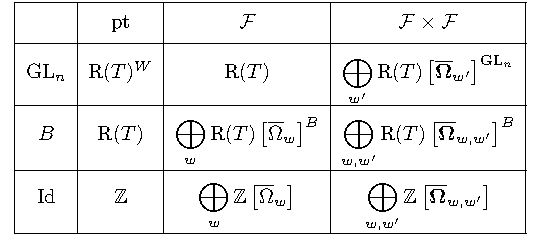
\includegraphics[width=8cm]{figures/table/table_module_initial.pdf}
      \caption{Initial case}
      \label{table:module_initial}        
\end{table}
\begin{table}[ht]
  \vspace{0cm}
    \centering  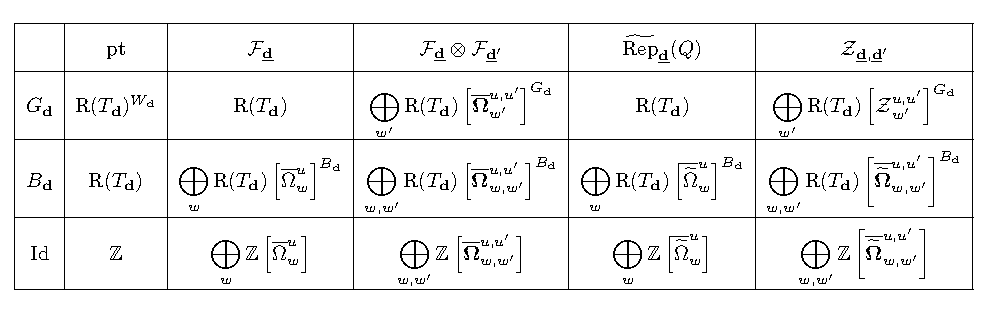
\includegraphics[width=15cm]{figures/table/table_module_relative.pdf}
      \caption{Relative case}
      \label{table:module_relative}        
\end{table}
\begin{table}[ht]
  \vspace{0cm}
    \centering  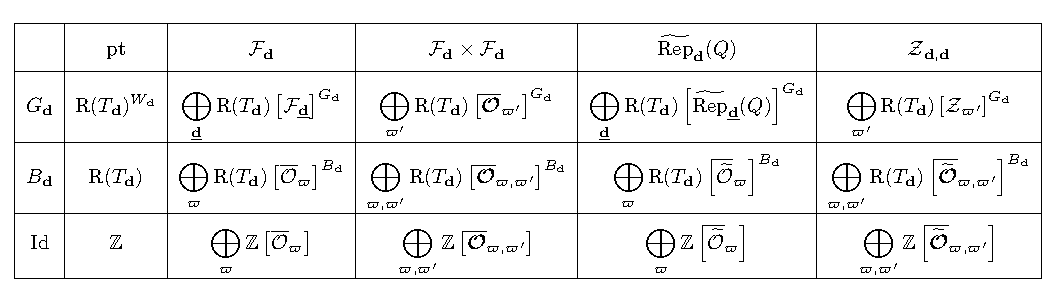
\includegraphics[width=15cm]{figures/table/table_module_absolute.pdf}
      \caption{Absolute case}
      \label{table:module_absolute}        
\end{table}
First, we work over Setting \ref{set:initial_case}.
\begin{eg}\label{eg:module-1-F}
The complete flag variety $\mathcal{F}$ has a stratification $\mathcal{F} = \sqcup_{w} \Omcell_{w}$. By extending the Bruhat order on $W$ to a total order $\preccurlyeq$, we get a cellular decomposition of $\mathcal{F}$:
% https://q.uiver.app/?q=WzAsMyxbMSwwLCJcXHN1YnNldGVxIFxcYmlnc3FjdXBfe3ggXFxwcmVjY3VybHllcSB3fVxcT21jZWxsX3t4fSBcXHN1YnNldGVxICJdLFswLDAsIjAgXFxzdWJzZXRlcSBcXE9tY2VsbF97XFxJZH0gXFxzdWJzZXRlcSJdLFsyLDAsIlxcc3Vic2V0ZXEgXFxiaWdzcWN1cF97eCB9XFxPbWNlbGxfe3h9ID1cXG1hdGhjYWx7Rn0iXSxbMSwwLCJcXGNkb3RzIiwzLHsic3R5bGUiOnsiYm9keSI6eyJuYW1lIjoibm9uZSJ9LCJoZWFkIjp7Im5hbWUiOiJub25lIn19fV0sWzAsMiwiXFxjZG90cyIsMyx7InN0eWxlIjp7ImJvZHkiOnsibmFtZSI6Im5vbmUifSwiaGVhZCI6eyJuYW1lIjoibm9uZSJ9fX1dXQ==
\[\begin{tikzcd}
	{0 \subseteq \Omcell_{\Id} \subseteq} & {\subseteq \bigsqcup_{x \preccurlyeq w}\Omcell_{x} \subseteq } & {\subseteq \bigsqcup_{x }\Omcell_{x} =\mathcal{F}}
	\arrow["\cdots"{marking}, draw=none, from=1-1, to=1-2]
	\arrow["\cdots"{marking}, draw=none, from=1-2, to=1-3]
\end{tikzcd}\]
By Theorem \ref{thm:cellular_fibration},
$$K^B(\mathcal{F}) \cong \bigoplus_{w} \Rpt(B) \left[ \overline{\Omcell}_{w} \right]^B \qquad K(\mathcal{F}) \cong \bigoplus_{w} \mathbb{Z} \left[ \overline{\Omcell}_{w} \right].$$
In particular,
\begin{equation*}
\begin{aligned}
  K^{\GL_n}(\mathcal{F} \times \mathcal{F}) \cong K^B(\mathcal{F})\cong\;& \bigoplus_{w} \Rpt(B) \cdot\Ind_B^{\GL_n} \left(\left[ \overline{\Omcell}_{w} \right]^B\right) \\ 
  \cong\;& \bigoplus_{w'} \Rpt(B)  \left[ \overline{\OOmcell}_{w'} \right]^{\GL_n}
\end{aligned}
\end{equation*}
\end{eg}


\begin{eg}\label{eg:module-2-FF}
$\mathcal{F} \times \mathcal{F}$ has many stratifications. Consider the stratification $\mathcal{F}\times \mathcal{F}= \sqcup_{w, w'\in W} \OOmcell_{w,w'}$. By extending the Bruhat order on $W \times W$ (i.e., $(x,x') \leq (w,w')$ if and only if $x \leq w$ and $x' \leq w'$) to a total order $\preccurlyeq$, we get a cellular decomposition of $\mathcal{F} \times \mathcal{F}$:
% https://q.uiver.app/?q=WzAsMyxbMSwwLCJcXHN1YnNldGVxIFxcYmlnc3FjdXBfeyh4LHgnKSBcXHByZWNjdXJseWVxICh3LHcnKX1cXE9PbWNlbGxfe3gseCd9IFxcc3Vic2V0ZXEgIl0sWzAsMCwiMCBcXHN1YnNldGVxIFxcT09tY2VsbF97XFxJZCxcXElkfSBcXHN1YnNldGVxIl0sWzIsMCwiXFxzdWJzZXRlcSBcXGJpZ3NxY3VwX3t4LHgnfVxcT09tY2VsbF97eCx4J30gPVxcbWF0aGNhbHtGfSBcXHRpbWVzIFxcbWF0aGNhbHtGfSJdLFsxLDAsIlxcY2RvdHMiLDMseyJzdHlsZSI6eyJib2R5Ijp7Im5hbWUiOiJub25lIn0sImhlYWQiOnsibmFtZSI6Im5vbmUifX19XSxbMCwyLCJcXGNkb3RzIiwzLHsic3R5bGUiOnsiYm9keSI6eyJuYW1lIjoibm9uZSJ9LCJoZWFkIjp7Im5hbWUiOiJub25lIn19fV1d
\[\begin{tikzcd}
	{0 \subseteq \OOmcell_{\Id,\Id} \subseteq} & {\subseteq \bigsqcup_{(x,x') \preccurlyeq (w,w')}\OOmcell_{x,x'} \subseteq } & {\subseteq \bigsqcup_{x,x'}\OOmcell_{x,x'} =\mathcal{F} \times \mathcal{F}}
	\arrow["\cdots"{marking}, draw=none, from=1-1, to=1-2]
	\arrow["\cdots"{marking}, draw=none, from=1-2, to=1-3]
\end{tikzcd}\]
By Theorem \ref{thm:cellular_fibration},
$$K^B(\mathcal{F} \times \mathcal{F}) \cong \bigoplus_{w,w'} \Rpt(B) \left[ \overline{\OOmcell}_{w,w'} \right]^B \qquad K(\mathcal{F} \times \mathcal{F}) \cong \bigoplus_{w,w'} \mathbb{Z} \left[ \overline{\OOmcell}_{w,w'} \right].$$

\end{eg}

\begin{eg}\label{eg:K-theory-by-induction}
For computing $K^{\GL_n}(\mathcal{F} \times \mathcal{F})$, consider the ($GL_n$-equivariant) stratification $\mathcal{F} \times \mathcal{F}= \sqcup_{w'} \OOmcell_{w'}$. Again, we get a cellular decomposition of $\pi_2: \mathcal{F} \times \mathcal{F} \longrightarrow \mathcal{F}$:
% https://q.uiver.app/?q=WzAsMyxbMSwwLCJcXHN1YnNldGVxIFxcYmlnc3FjdXBfe3gnIFxccHJlY2N1cmx5ZXEgdyd9XFxPT21jZWxsX3t4J30gXFxzdWJzZXRlcSAiXSxbMCwwLCIwIFxcc3Vic2V0ZXEgXFxPT21jZWxsX3tcXElkfSBcXHN1YnNldGVxIl0sWzIsMCwiXFxzdWJzZXRlcSBcXGJpZ3NxY3VwX3t4J31cXE9PbWNlbGxfe3gnfSA9XFxtYXRoY2Fse0Z9IFxcdGltZXMgXFxtYXRoY2Fse0Z9Il0sWzEsMCwiXFxjZG90cyIsMyx7InN0eWxlIjp7ImJvZHkiOnsibmFtZSI6Im5vbmUifSwiaGVhZCI6eyJuYW1lIjoibm9uZSJ9fX1dLFswLDIsIlxcY2RvdHMiLDMseyJzdHlsZSI6eyJib2R5Ijp7Im5hbWUiOiJub25lIn0sImhlYWQiOnsibmFtZSI6Im5vbmUifX19XV0=
\[\begin{tikzcd}
	{0 \subseteq \OOmcell_{\Id} \subseteq} & {\subseteq \bigsqcup_{x' \preccurlyeq w'}\OOmcell_{x'} \subseteq } & {\subseteq \bigsqcup_{x'}\OOmcell_{x'} =\mathcal{F} \times \mathcal{F}}
	\arrow["\cdots"{marking}, draw=none, from=1-1, to=1-2]
	\arrow["\cdots"{marking}, draw=none, from=1-2, to=1-3]
\end{tikzcd}\]
By Theorem \ref{thm:cellular_fibration} and Example \ref{eg:contracted_product_FF}, we get
\begin{equation*}
\begin{aligned}
  K^{\GL_n}(\mathcal{F} \times \mathcal{F})\cong\;& \bigoplus_{w'} K^{\GL_n}(\OOmcell_{w'})  \\ 
  \cong\;& \bigoplus_{w'} K^B(\Omcell_{w'})  \\ 
  \cong\;& \bigoplus_{w'} \Rpt(B) \left[ \overline{\OOmcell}_{w'} \right]^{\GL_n} \\ 
\end{aligned}
\end{equation*}
\end{eg}
The general case can be solved by the same method.
\begin{eg}
By repeating Example \ref{eg:K-initial-1} to \ref{eg:K-initial-4}, we get
$$\Rpt(N_{\dimvec{d}}) \cong \Rpt(\Id) \cong \mathbb{Z} \qquad \Rpt(B_{\dimvec{d}}) \cong \Rpt(T_{\dimvec{d}}) \cong \mathbb{Z}\!\left[ e_1^{\pm 1},\ldots,e_{\abdimvec{d}}^{\pm 1} \right]$$
$$ \Rpt(G_{\dimvec{d}}) \cong \Rpt(T_{\dimvec{d}})^{\Wd} \cong \mathbb{Z}\!\left[ e_1^{\pm 1},\ldots,e_{\abdimvec{d}}^{\pm 1} \right]^{\Wd}$$
The induction formula tells us 
$$K^{G_{\dimvec{d}}} (\mathcal{F}_{\ftdimvec{d}}) \cong K^{B_{\dimvec{d}}} (\pt) =\Rpt (B_{\dimvec{d}}) \cong \mathbb{Z}\!\left[ e_1^{\pm 1},\ldots,e_{\abdimvec{d}}^{\pm 1} \right].$$
By repeating Example \ref{eg:module-1-F} to \ref{eg:module-2-FF}, we get

\begin{equation*}
\begin{aligned}
&K^{B_{\dimvec{d}}}(\mathcal{F}_{\ftdimvec{d}}) \cong \bigoplus_{w} \Rpt(B_{\dimvec{d}}) \left[ \overline{\Omcell}_{w}^{u} \right]^{B_{\dimvec{d}}} \qquad &&K(\mathcal{F}_{\ftdimvec{d}}) \cong \bigoplus_{w} \mathbb{Z} \left[ \overline{\Omcell}_{w}^{u} \right]\\
&K^{G_{\dimvec{d}}}(\mathcal{F}_{\ftdimvec{d}} \times \mathcal{F}_{\ftdimvec{d}'}) \cong \bigoplus_{w'} \Rpt(B_{\dimvec{d}}) \left[ \overline{\OOmcell}_{w'}^{u,u'} \right]^{G_{\dimvec{d}}}\\
&K^{B_{\dimvec{d}}}(\mathcal{F}_{\ftdimvec{d}} \times \mathcal{F}_{\ftdimvec{d}'}) \cong \bigoplus_{w,w'} \Rpt(B_{\dimvec{d}}) \left[ \overline{\OOmcell}_{w,w'}^{u,u'} \right]^{B_{\dimvec{d}}} \qquad &&K(\mathcal{F}_{\ftdimvec{d}} \times \mathcal{F}_{\ftdimvec{d}'}) \cong \bigoplus_{w,w'} \mathbb{Z} \left[ \overline{\OOmcell}_{w,w'}^{u,u'} \right]\\
\end{aligned}
\end{equation*}

Since 
$$\mathcal{F}_{\dimvec{d}}= \bigsqcup_{\ftdimvec{d}}\mathcal{F}_{\ftdimvec{d}}\qquad \mathcal{F}_{\dimvec{d}} \times \mathcal{F}_{\dimvec{d}} = \bigsqcup_{\ftdimvec{d},\ftdimvec{d}'}\mathcal{F}_{\ftdimvec{d}} \times \mathcal{F}_{\ftdimvec{d}'}$$
as topological spaces, we get $K$-theory of $\mathcal{F}_{\dimvec{d}}$ and $\mathcal{F}_{\dimvec{d}} \times \mathcal{F}_{\dimvec{d}}$ for free. (See Table???)
\end{eg}

The calculations of incidence spaces use the same method we introduced in Example \ref{eg:K-theory-by-induction}.

\begin{eg}
We compute $G_{\dimvec{d}}$-equivariant $K$-theory of the Steinberg variety in this example.
\begin{equation*}
\begin{aligned}
  K^{G_{\dimvec{d}}}(\St_{\ftdimvec{d},\ftdimvec{d}'})\cong\;& \bigoplus_{w'} K^{G_{\dimvec{d}}}(\preimage{\OOmcell}_{w'}^{u,u'})  \\ 
  \cong\;& \bigoplus_{w'} K^{G_{\dimvec{d}}}(\OOmcell_{w'}^{u,u'})  \\ 
  \cong\;& \bigoplus_{w'} K^{B_{\dimvec{d}}}(\Omcell_{w'}^{u,u'})  \\ 
  \cong\;& \bigoplus_{w'} \Rpt(B_{\dimvec{d}}) \left[ \overline{\preimage{\OOmcell}}_{w'}^{u,u'} \right]^{G_{\dimvec{d}}} \\ 
\end{aligned}
\end{equation*}
\end{eg}

Now we've done with the module structure. The equivariant cohomology theory can be also computed in the exact same way, see \cite[Chapter 7]{przezdziecki2015geometric}.

%%%%%%%%%%%%%%%%%%%%%%%%%%%%%%%%%%%%%%%%%%%%%%%%%%%%%%%%%%%%%%%%%%%%%%%%%%%%%%%%%%%%%%%%%%%%%
\chapter{Localization theorem}\label{chap:localization}
We have already gotten the module structure of $K$-theories. However, these basis behave badly with the convolution product (will be introduced in Section \ref{sec:convolution}), because "the information is not concentrated enough". In this chapter we will introduce another basis, which "concentrate information in the $T$-fixed points". The localization formula describe the transition matrix of two basis. Readers with topological background can compare the localization theorem with the Poincaré-Hopf theorem.


\section{Euler class}\label{sec:euler_class}
In the category of coherent sheaf, the "proper base change" is usually not true. In order to describe the defect of the diagram, we introduce the Euler class.

\begin{defn}[Euler class, for $K$-group]
Let $X$ be a $G$-variety, and $\mathcal{T}$ be a $G$-equivariant vector bundle over $X$. The Euler class is defined by
$$\eu(\mathcal{T}):= \sum_{k=0}^{\infty} (-1)^k \left[ \Lambda^{k} \mathcal{T}^* \right] \in \Rpt(G) $$
\end{defn}

In practice, $X$ are points and $G$ is a torus. In that case, since we know the representation of a torus (see Example \ref{eg:K-initial-2}), the Euler class can be explicitly written down. For example, ($X=\pt$)
\begin{equation*}
\begin{aligned}
  &\eu\left( 1 \right)=  1\\ 
    &\eu\left( \frac{e_1}{e_2} \right)=  1-\frac{e_2}{e_1}\\ 
      &\eu\left(\frac{e_1}{e_2}+\frac{e_2}{e_3}+\frac{e_3}{e_1} \right)=  \left(1-\frac{e_2}{e_1}\right)\left(1-\frac{e_3}{e_2}\right)\left(1-\frac{e_1}{e_3}\right)\\ 
\end{aligned}
\end{equation*}
Here we confuse the notation of $\Rpt(T)$ and $\Rep(T)$: the elements inside the bracket of Euler class should be viewed as a vector bundle rather than a linear combination of coherent sheaves. 

\begin{warning}
Compared with usual Euler class, some properties are kept in $K$-theory version, while some are not. For example, for line bundles $\mathcal{L}$, $\mathcal{L}_1$, $\mathcal{L}_2$ over $X$,
\begin{equation*}
\begin{aligned}
  &  \eu(\mathcal{T} \oplus \mathcal{T}') \cong \eu(\mathcal{T}) \cdot \eu(\mathcal{T}'),            \\ 
  & \eu(\mathcal{L}_1 \otimes \mathcal{L}_2) \neq \eu(\mathcal{L}_1 )+\eu( \mathcal{L}_2) \qquad \eu(\mathcal{L}^{*}) \neq -\eu(\mathcal{L}).
\end{aligned}
\end{equation*}
\end{warning}

\begin{remark}
We also have equivariant Euler class for cohomology theory, see \cite[Chapter 9]{przezdziecki2015geometric}, ??? for more details. In particular, for any $T$-representation $\mathcal{T}$ with weight space decomposition $\mathcal{T}^{*} = \oplus \mathcal{T}_{\lambda}^{*}$, the Euler class of $\mathcal{T}$ (for cohomology theory) is defined by
$$\eu'(\mathcal{T}):= \prod_{\lambda \in X^{*}(T)} \lambda^{\dim \mathcal{T}_{\lambda}^{*}} \in \Spt(T) $$
where $X^{*}(T)$ embeds in $\Spt(T)$ by
$$X^{*}(T) \longrightarrow \Spt(T) \qquad \sum_{i}k_i \varepsilon_i \longmapsto \sum_{i}k_i \lambda_i.$$
For example,
\begin{equation*}
\begin{aligned}
  &\eu'\left( 1 \right)=  1\\ 
    &\eu'\left( \frac{e_1}{e_2} \right)=  \lambda_2-\lambda_1\\ 
      &\eu'\left(\frac{e_1}{e_2}+\frac{e_2}{e_3}+\frac{e_3}{e_1} \right)=  \left(\lambda_2-\lambda_1\right)\left(\lambda_3-\lambda_2\right)\left(\lambda_1-\lambda_3\right)\\ 
\end{aligned}
\end{equation*}
\end{remark}

\section{Statement}\label{sec:statement_localization}
We first state one general theorem, which will be connected with both localization formula and excess intersection formula.

\begin{theorem}[{Excess base change, \cite[Théorème 3.1]{thomason1993k}}]\label{thm:excess_base_change}
Let \eqref{eq:excess_base_change} be a Cartesian square of $G$-varieties, $\phi$, $\varphi$ are regular embeddings and $f,g$ are of globally finite $\Tor$-dimension. Denote $\mathcal{N}_{\phi}$ and $\mathcal{N}_{\varphi}$ as the normal cone of $\phi$, $\varphi$ respectively, and $\mathcal{T}:=(g^{*}\mathcal{N}_{\varphi})/\mathcal{N}_{\phi}$ as a vector bundle over $W$.
\begin{equation}\label{eq:excess_base_change}
% https://q.uiver.app/?q=WzAsNyxbMSwxLCJXIl0sWzMsMSwiWiJdLFszLDIsIlgiXSxbMSwyLCJZIl0sWzQsMCwiXFxtYXRoY2Fse059X3tcXHZhcnBoaX0iXSxbMiwwLCJnXnsqfVxcbWF0aGNhbHtOfV97XFx2YXJwaGl9Il0sWzAsMCwiXFxtYXRoY2Fse059X3tcXHBoaX0iXSxbMywyLCJmIl0sWzEsMiwiXFx2YXJwaGkiXSxbMCwxLCJnIl0sWzAsMywiXFxwaGkiLDJdLFs0LDEsIiIsMCx7InN0eWxlIjp7ImhlYWQiOnsibmFtZSI6Im5vbmUifX19XSxbNSwwLCIiLDAseyJzdHlsZSI6eyJoZWFkIjp7Im5hbWUiOiJub25lIn19fV0sWzYsMCwiIiwwLHsic3R5bGUiOnsiaGVhZCI6eyJuYW1lIjoibm9uZSJ9fX1dXQ==
\begin{tikzcd}[row sep={between origins,20mm},column sep={between origins,5mm}]
	{\mathcal{N}_{\phi}} && {g^{*}\mathcal{N}_{\varphi}} &[10mm]& {\mathcal{N}_{\varphi}} \\[-12mm]
	& N && Z \\
	& Y && X
	\arrow["f", from=3-2, to=3-4]
	\arrow["\varphi", from=2-4, to=3-4]
	\arrow["g", from=2-2, to=2-4]
	\arrow["\phi"', from=2-2, to=3-2]
	\arrow[no head, from=1-5, to=2-4]
	\arrow[no head, from=1-3, to=2-2]
	\arrow[no head, from=1-1, to=2-2]
\end{tikzcd}
\end{equation}

For any $\alpha \in K^G(Z)$, we have the \textbf{excess base change formula}:
$$f^* \circ \varphi_{*}(\alpha)=\phi_{*} \left( \eu(\mathcal{T})\cdot g^*(\alpha)\rule{0mm}{4mm}  \right) \qquad \text{ in }K^{G}(Y)$$


\end{theorem}

By applying Theorem \ref{thm:excess_base_change} to the Cartesian square \eqref{eq:fake_localization_formula}, we get the (fake) localization formula:
\begin{equation}\label{eq:fake_localization_formula}
% https://q.uiver.app/?q=WzAsNCxbMSwwLCJYXlQiXSxbMCwwLCJYXlQiXSxbMCwxLCJYXlQiXSxbMSwxLCJYIl0sWzAsMywiaSJdLFsyLDMsImkiXSxbMSwwLCJcXElkIl0sWzEsMiwiXFxJZCIsMl1d
\begin{tikzcd}
	{X^T} & {X^T} \\
	{X^T} & X
	\arrow["i", from=1-2, to=2-2]
	\arrow["i", from=2-1, to=2-2]
	\arrow["\Id", from=1-1, to=1-2]
	\arrow["\Id"', from=1-1, to=2-1]
\end{tikzcd}
\end{equation}

\begin{proposition}[Fake localization formula]
For a smooth $T$-variety $X$ with finite fixed points $\{x_1,\ldots,x_m \}$, denote $i:X^T \longrightarrow X$ and $i_k: \{x_k\} \longrightarrow X$ as embeddings. For any $\beta \in K^T(X^T)$, $\beta_k \in K^T(\{x_k\})$, we have formulas
$$i^*i_* \beta =\eu \left( \bigoplus_k T_{x_k}X \right) \cdot \beta \qquad i_{k}^*i_{k,*} \beta =\eu \left( T_{x_k}X \right) \cdot \beta_k.$$


\end{proposition}

This proposition is not as powerful as it is supposed to be, but it explains some technical details in the localization theorem and localization formula. First, we would like to work on a base ring where Euler classes are invertible, so we denote the curly font as everything in the fraction field.
\begin{equation*}
\begin{aligned}
  \Rptc(T):=\;& \Frac\!\big(\!\Rpt(T)\big) \qquad & \Kcurl^T(X):=\;& K^T(X) \otimes_{\Rpt(T)}\Rptc(T)  \\ 
  \Sptc(T):=\;& \Frac\!\big(\!\Spt(T)\big) \qquad & \Hcurl_{T}^{*}(X):=\;& H_{T}^{*}(X) \otimes_{\Spt(T)}\Sptc(T)  \\
\end{aligned}
\end{equation*}

Now we can do linear algebras and discuss about the actual basis:
\begin{theorem}[{Localization theorem, \cite[Theorem 10.1]{przezdziecki2015geometric} or \cite[Corollary 5.11.3]{chriss1997representation}}] \label{thm:localization_theorem}
Let $X$ be a smooth $T$-variety,  $i:X^T \longrightarrow X$ be the embedding. The morphisms $i_*$, $i^*$ are isomorphism after tensored over the fraction field, i.e.,
% https://q.uiver.app/?q=WzAsNixbMSwwLCJcXEtjdXJsXlQoWCkiXSxbMCwwLCJcXEtjdXJsXlQoWF5UKSJdLFsyLDAsIlxcS2N1cmxeVChYXlQpIl0sWzAsMSwiXFxIY3VybF97VH1eeyp9KFheVCkiXSxbMSwxLCJcXEhjdXJsX3tUfV57Kn0oWCkiXSxbMiwxLCJcXEhjdXJsX3tUfV57Kn0oWF5UKSJdLFswLDIsImleKiJdLFszLDQsImlfKiJdLFs0LDUsImleKiJdLFsxLDAsImlfKiJdXQ==
\[\begin{tikzcd}[row sep=0mm]
	{\Kcurl^T(X^T)} & {\Kcurl^T(X)} & {\Kcurl^T(X^T)} \\
	{\Hcurl_{T}^{*}(X^T)} & {\Hcurl_{T}^{*}(X)} & {\Hcurl_{T}^{*}(X^T)}
	\arrow["{i^*}", from=1-2, to=1-3]
	\arrow["{i_*}", from=2-1, to=2-2]
	\arrow["{i^*}", from=2-2, to=2-3]
	\arrow["{i_*}", from=1-1, to=1-2]
\end{tikzcd}\]
are isomorphism as $\mathcal{R}(T)$ or $\mathcal{S}(T)$-modules.
\end{theorem}

The genuine localization formula is stated as follows.

\begin{theorem}[{Localization formula, \cite[Theorem 10.2]{przezdziecki2015geometric} or \cite[Proposition 6]{edidin1998localization}}]\label{thm:localization_formula}
For a smooth $T$-variety $X$ with finite fixed points $\{x_1,\ldots,x_m \}$, denote $i_k: \{x_k\} \longrightarrow X$ as embeddings. For any $\alpha \in \Kcurl^T(X)$, we have formula
$$\alpha= \sum_{k=1}^{m} \eta_k \cdot i_{k,*}i_{k}^* \alpha $$
where $\eta_k:= \left(\!\rule{0mm}{3.5mm} \eu(T_{x_k}X) \right)^{-1} \in \Rptc(T)$.

More generally, suppose $f: Y \hookrightarrow X$ is a $T$-equivariant closed subvariety with finite fixed points $\{x_1,\ldots,x_{m'} \}$, denote $i'_k: \{x_k\} \longrightarrow Y$ as embeddings. For any $\beta \in \Kcurl^T(Y)$, we have formula
$$\beta= \sum_{k=1}^{m} \eta_k \cdot i'_{k,*}i_{k}^* f_{*} \beta. $$

\end{theorem}

Let us unravel Theorem \ref{thm:localization_formula} a little bit. For the closed $T$-equivariant subset $Z$ of $Y$, denote $[Z]_X^T \in K^T(X)$, $[Z]_Y^T \in K^T(Y)$, $[x_k]_Y^T \in K^T(Y)$. Substitute the localization formula, we get
\begin{equation*}
\begin{aligned}\
   [Z]_Y^T=\;& \sum_{k=1}^{m} \eta_k \cdot i'_{k,*}i_{k}^* f_{*} [Z]_Y^T&& \\
   =\;& \sum_{k=1}^{m} \eta_k \cdot i'_{k,*}\left(i_{k}^* [Z]_X^T \cdot 1_{\Rpt(T)}\right) && \text{by definition of $[Z]_X^T$}\\
   =\;& \sum_{k=1}^{m} \eta_k \cdot \left(i_{k}^* [Z]_X^T\right) \cdot\left( i'_{k,*} 1_{\Rpt(T)}\right) && \text{$i'_{k,*}$ is a $\Rpt(T)$-module homomorphism}\hspace{-14mm}\\
   =\;& \sum_{k=1}^{m} \eta_k \cdot \left(i_{k}^* [Z]_X^T\right) \cdot[x_k]_Y^T && \text{by definition of $[x_k]_Y^T$}\\
\end{aligned}
\end{equation*}
When $Z$ is smooth at $x_k$,\footnote{The smoothness guaranteed the regular embedding condition in Theorem \ref{thm:excess_base_change}.} denote $g: Z \hookrightarrow X$ and $j_k: \{x_k\} \longrightarrow Z$, 
\begin{equation*}
\begin{aligned}\
   i_{k}^* [Z]_X^T=\;& i_{k}^* g_* \big(  \pi_Z^* 1_{\Rpt(T)} \big) &&\\
   =\;& \eu \left( j_k^* N_Z X  \right) \cdot j_k^* \big(  \pi_Z^* 1_{\Rpt(T)} \big) \qquad&& \text{by excess base change}\\
   =\;& \eu \left( \frac{T_{x_k}X}{T_{x_k}Z}  \right) \cdot  1_{\Rpt(T)}&& \pi_Z \circ j_k = \Id_{\pt} \\
   =\;& \frac{\eu \left(T_{x_k}X\right)}{\eu \left(T_{x_k}Z\right)} && \text{ $\Rep(T)$ is semisimple} \\
\end{aligned}
\end{equation*}
Therefore, the coefficient before $[x_k]_Y^T$ is 
$$\eta_k \cdot \left(i_{k}^* [Z]_X^T\right) = \frac{1}{\eu \left(T_{x_k}X\right)}\cdot\frac{\eu \left(T_{x_k}X\right)}{\eu \left(T_{x_k}Z\right)}=\frac{1}{\eu \left(T_{x_k}Z\right)}.$$
In other word, we computed the transition matrix between two basis, where the matrix coefficient is roughly the inverse of the Euler class. Keep this is mind, and let us see applications now.

\section{Application: change of basis}
Before we really start working, let us make a shorthand for the basis and the Euler class.

\begin{defn}[Another basis]
For $\ww$, $\ww'$, $x \in \WWd$, denote
\begin{equation*}
\begin{aligned}
  \psi_{\ww}:=\;& \left[\{F_{\ww}\} \right]^{T_{\dimvec{d}}} = (i_{\ww})_{*} 1_{\Rpt(T_{\dimvec{d}})} && \in K^{T_{\dimvec{d}}} (\mathcal{F}_{\dimvec{d}}) \\ 
  \psi_{\ww}^{x}:=\;& \left[\{F_{\ww}\} \right]^{T_{\dimvec{d}}} = (i_{\ww}^x)_{*} 1_{\Rpt(T_{\dimvec{d}})} && \in K^{T_{\dimvec{d}}} (\overline{\Ocell}_x) \\ 
  \psi_{\ww,\ww'}:=\;& \left[\{F_{\ww,\ww'}\} \right]^{T_{\dimvec{d}}} = (i_{\ww,\ww'})_{*} 1_{\Rpt(T_{\dimvec{d}})} && \in K^{T_{\dimvec{d}}} (\mathcal{F}_{\dimvec{d}} \times \mathcal{F}_{\dimvec{d}} ) \\ 
  \psi_{\ww,\ww'}^{x}:=\;& \left[\{F_{\ww,\ww'}\} \right]^{T_{\dimvec{d}}} = (i_{\ww,\ww'}^{x})_{*} 1_{\Rpt(T_{\dimvec{d}})} && \in K^{T_{\dimvec{d}}} (\overline{\OOcell}_x) \\ 
\end{aligned}
\end{equation*}
The same symbols are used for 
$$\preimage{\psi}_{\ww} \in K^{T_{\dimvec{d}}} \left( \RRep_{\dimvec{d}}(Q) \right)  \quad  \preimage{\psi}_{\ww}^{x} \in K^{T_{\dimvec{d}}} \left( \overline{\preimage{\Ocell}}_x \right)  \quad  \preimage{\psi}_{\ww,\ww'} \in K^{T_{\dimvec{d}}} (\St_{\dimvec{d}})  \quad  \preimage{\psi}_{\ww,\ww'}^{x} \in K^{T_{\dimvec{d}}} (\St_x).$$
Also, we use underline to twist subscripts, like $\underline{\psi}_{\ww,\ww'}:=\psi_{\ww,\ww\ww'}$.
\end{defn}

By Theorem \ref{thm:localization_theorem},
\begin{equation*}
\begin{aligned}
   \Kcurl^{T_{\dimvec{d}}} (\mathcal{F}_{\dimvec{d}}) \cong\;& \bigoplus_{\ww} \Rptc(T_{\dimvec{d}}) \psi_{\ww}\qquad & \Kcurl^{T_{\dimvec{d}}} (\mathcal{F}_{\dimvec{d}} \times \mathcal{F}_{\dimvec{d}} ) \cong\;& \bigoplus_{\ww,\ww'} \Rptc(T_{\dimvec{d}}) \psi_{\ww,\ww'} \\ 
   \Kcurl^{T_{\dimvec{d}}} \left(\RRep_{\dimvec{d}}(Q)\right) \cong\;& \bigoplus_{\ww} \Rptc(T_{\dimvec{d}}) \preimage{\psi}_{\ww} & \Kcurl^{T_{\dimvec{d}}} (\St_{\dimvec{d}} ) \cong\;& \bigoplus_{\ww,\ww'} \Rptc(T_{\dimvec{d}}) \preimage{\psi}_{\ww,\ww'}. \\ 
\end{aligned}
\end{equation*}

\begin{defn}[Shorthand for Euler class]
For $\ww$, $\ww'$, $x \in \WWd$, denote the Euler class in $\Rpt(T_{\dimvec{d}})$:
\begin{equation*}
\begin{aligned}
  \Lambda_{\ww}:=\;& \eu\left(\mathcal{T}_{\ww}\right) \quad& \Lambda_{\ww}^x:=\;& \eu\left(\mathcal{T}_{\ww}^x\right) \quad& \Lambda_{\ww,\ww'}^x:=\;& \eu\left(\mathcal{T}_{\ww,\ww'}^x \right) \\ 
    \preimage{\Lambda}_{\ww}:=\;& \eu\left(\preimage{\mathcal{T}}_{\ww}\right) \quad& \preimage{\Lambda}_{\ww}^x:=\;& \eu\left(\preimage{\mathcal{T}}_{\ww}^x\right) \quad& \preimage{\Lambda}_{\ww,\ww'}^x:=\;& \eu\left(\preimage{\mathcal{T}}_{\ww,\ww'}^x\right)  \\ 
\end{aligned}
\end{equation*}
For completeness, denote
$$\Lambda_{\ww,\ww'}:=\eu\left(\mathcal{T}_{\ww,\ww'}\right) \qquad \preimage{\Lambda}_{\ww,\ww'}:=\eu\left(\preimage{\mathcal{T}}_{\ww,\ww'}\right).$$
Also, we use underline to twist subscripts.
\end{defn}

Now we can compute the transition matrix of two basis.

\begin{eg}
Let $X=Y=\mathcal{F}_{\dimvec{d}}$, $T=T_{\dimvec{d}}$, $i_{\ww}: \{F_{\ww}\} \hookrightarrow \mathcal{F}_{\dimvec{d}}$ be the embedding, $y \in \Wd$, we get
$$\left[  \overline{\Omcell}_{y}^{u} \right]^{T_{\dimvec{d}}}= \sum_{w \leq y} \Lambda_{wu}^{-1}\left(  i_{wu}^{*} \left[  \overline{\Omcell}_y^{u} \right]^{T_{\dimvec{d}}} \right) \cdot \psi_{wu}.$$
When $\overline{\Omcell}_{y}^{u}$ is smooth at $F_{wu}$, $\Lambda_{wu}^{-1}\left(  i_{wu}^{*} \left[  \overline{\Omcell}_y^{u} \right]^{T_{\dimvec{d}}} \right) = \left( \eu \left( T_{F_{wu}} \overline{\Omcell}_{y}^{u}  \right)\rule{0mm}{4mm} \right)^{-1} = \left(\Lambda_{wu}^{yu}\right)^{-1}$. Especially, for $s \in \Pi_{\dimvec{d}}$,
\begin{equation*}
\begin{aligned}
  \left[  \overline{\Omcell}_{\Id}^{u} \right]^{T_{\dimvec{d}}}=\;&  \left( \Lambda_{u}^{u}  \right)^{-1} \psi_{u}=\psi_{u} \\
  \left[  \overline{\Omcell}_{s}^{u} \right]^{T_{\dimvec{d}}}=\;&  \left( \Lambda_{u}^{su}  \right)^{-1} \psi_{u} + \left( \Lambda_{su}^{su}  \right)^{-1} \psi_{su} \\
  \left[  \mathcal{F}_{u} \right]^{T_{\dimvec{d}}}=\;&  \sum_{w} \Lambda_{wu}^{-1} \psi_{wu} \\
  \left[  \mathcal{F}_{\dimvec{d}} \right]^{T_{\dimvec{d}}}=\;&  \sum_{\ww} \Lambda_{\ww}^{-1} \psi_{\ww} \\  
\end{aligned}
\end{equation*}
Also, for $s \in \Pi$,
$$
\left[  \overline{\Ocell}_s \right]^{T_{\dimvec{d}}}=
\begin{cases}
\left( \Lambda_{\Id}^{s}  \right)^{-1} \psi_{\Id} + \left( \Lambda_{s}^{s}  \right)^{-1} \psi_{s}, &s \in \Pi_{\dimvec{d}}\\
\psi_{s}, &s \notin \Pi_{\dimvec{d}}
\end{cases}
$$
\end{eg}

\begin{eg}
Let $X=Y=\RRep_{\dimvec{d}}(Q)$, $T=T_{\dimvec{d}}$, $i_{\ww}: \{(\rho_0, F_{\ww})\} \hookrightarrow \RRep_{\dimvec{d}}(Q)$ be the embedding, $y \in \Wd$, we get
$$\left[  \overline{\preimage{\Omcell}}_{y}^{u} \right]^{T_{\dimvec{d}}}= \sum_{w \leq y} \preimage{\Lambda}_{wu}^{-1}\left(  i_{wu}^{*} \left[  \overline{\preimage{\Omcell}}_y^{u} \right]^{T_{\dimvec{d}}} \right) \cdot \preimage{\psi}_{wu}.$$
When $\overline{\preimage{\Omcell}}_{y}^{u}$ is smooth at $F_{wu}$, $\preimage{\Lambda}_{wu}^{-1}\left(  i_{wu}^{*} \left[  \overline{\preimage{\Omcell}}_y^{u} \right]^{T_{\dimvec{d}}} \right) = \left( \eu \left( T_{F_{wu}} \overline{\preimage{\Omcell}}_{y}^{u}  \right)\rule{0mm}{4mm} \right)^{-1} = \left(\preimage{\Lambda}_{wu}^{yu}\right)^{-1}$. Especially, for $s \in \Pi_{\dimvec{d}}$,
\begin{equation*}
\begin{aligned}
  \left[  \overline{\preimage{\Omcell}}_{\Id}^{u} \right]^{T_{\dimvec{d}}}=\;&  \left( \preimage{\Lambda}_{u}^{u}  \right)^{-1} \preimage{\psi}_{u}=\preimage{\psi}_{u} \\
  \left[  \overline{\preimage{\Omcell}}_{s}^{u} \right]^{T_{\dimvec{d}}}=\;&  \left( \preimage{\Lambda}_{u}^{su}  \right)^{-1} \preimage{\psi}_{u} + \left( \preimage{\Lambda}_{su}^{su}  \right)^{-1} \preimage{\psi}_{su} \\
  \left[  \RRep_{\ftdimvec{d}}(Q) \right]^{T_{\dimvec{d}}}=\;&  \sum_{w} \preimage{\Lambda}_{wu}^{-1} \preimage{\psi}_{wu} \\
  \left[  \RRep_{\dimvec{d}}(Q) \right]^{T_{\dimvec{d}}}=\;&  \sum_{\ww} \preimage{\Lambda}_{\ww}^{-1} \preimage{\psi}_{\ww} \\  
\end{aligned}
\end{equation*}
Also, for $s \in \Pi$,
$$
\left[  \overline{\preimage{\Ocell}}_s \right]^{T_{\dimvec{d}}}=
\begin{cases}
\left( \preimage{\Lambda}_{\Id}^{s}  \right)^{-1} \preimage{\psi}_{\Id} + \left( \preimage{\Lambda}_{s}^{s}  \right)^{-1} \preimage{\psi}_{s}, &s \in \Pi_{\dimvec{d}}\\
\preimage{\psi}_{s}, &s \notin \Pi_{\dimvec{d}}
\end{cases}
$$
\end{eg}

\begin{eg}
Let $X=Y=\mathcal{F}_{\dimvec{d}} \times \mathcal{F}_{\dimvec{d}}$, $T=T_{\dimvec{d}}$, $s \in \Pi$. Since $\overline{\OOcell}_s$ is smooth, we get
$$\left[  \overline{\OOcell}_s \right]^{T_{\dimvec{d}}}= \sum_{\ww \in \WWd} \left( \Lambda_{\ww,\ww s}^{s} \right)^{-1} \psi_{\ww,\ww s} +  \sum_{\substack{\ww \in \WWd \\ \ww s \ww^{-1} \in \Wd}} \left( \Lambda_{\ww,\ww}^{s} \right)^{-1} \psi_{\ww,\ww}.$$
One can also write $\left[  \overline{\OOcell}_{\ww} \right]$ in terms of $\Rptc(T_{\dimvec{d}})$-linear combination of those $\psi_{\ww,\ww'}$.

%$$\left[  \overline{\OOmcell}_{y,y'}^{u,u'} \right]^{T_{\dimvec{d}}}= \sum_{(w,w') \leq (y,y')} \Lambda_{wu,ww'u'}^{-1}\left(  i_{wu,ww'u'}^{*} \left[  \overline{\OOmcell}_{y,y'}^{u,u'} \right]^{T_{\dimvec{d}}} \right) \cdot \psi_{wu,ww'u'}.$$
%When $\overline{\OOmcell}_{y,y'}^{u,u'}$ is smooth at $F_{wu,ww'u'}$, $\Lambda_{wu,ww'u'}^{-1}\left(  i_{wu,ww'u'}^{*} \left[  \overline{\OOmcell}_{y,y'}^{u,u'} \right]^{T_{\dimvec{d}}} \right) = \left( \eu \left( T_{F_{wu,ww'u'}} \overline{\OOmcell}_{y,y'}^{u,u'}  \right)\rule{0mm}{4mm} \right)^{-1}$. Especially, for $s \in \Pi_{\dimvec{d}}$,
%%%%haven't change the result
%\begin{equation*}
%\begin{aligned}
%  \left[  \overline{\OOmcell}_{\Id,\Id}^{u,u'} \right]^{T_{\dimvec{d}}}=\;&  \left( \Lambda_{u}^{u}  \right)^{-1} \psi_{u}=\psi_{u} \\
%  \left[  \overline{\OOmcell}_{\Id,s}^{u,u'} \right]^{T_{\dimvec{d}}}=\;&  \left( \Lambda_{u}^{su}  \right)^{-1} \psi_{u} + \left( \Lambda_{su}^{su}  \right)^{-1} \psi_{su} \\
%  \left[  \mathcal{F}_{u} \right]^{T_{\dimvec{d}}}=\;&  \sum_{w} \Lambda_{wu}^{-1} \psi_{wu} \\
%  \left[  \mathcal{F}_{\dimvec{d}} \right]^{T_{\dimvec{d}}}=\;&  \sum_{\ww} \Lambda_{\ww}^{-1} \psi_{\ww} \\  
%\end{aligned}
%\end{equation*}
%Also, for $s \in \Pi$,
%$$
%\left[  \overline{\OOcell}_s \right]^{T_{\dimvec{d}}}=
%\begin{cases}
%\left( \Lambda_{\Id}^{s}  \right)^{-1} \psi_{\Id} + \left( \Lambda_{s}^{s}  \right)^{-1} \psi_{s}, &s \in \Pi_{\dimvec{d}}\\
%\psi_{s}, &s \notin \Pi_{\dimvec{d}}
%\end{cases}
%$$
\end{eg}

\begin{eg}
Let $X=\Rep_{\dimvec{d}}(Q) \times \mathcal{F}_{\dimvec{d}} \times \mathcal{F}_{\dimvec{d}}$, $Y=\St_{\dimvec{d}}$, $T=T_{\dimvec{d}}$, $s \in \Pi$. Since $\St_s$ is smooth, we get
$$\left[  \St_s \right]^{T_{\dimvec{d}}}= \sum_{\ww \in \WWd} \left( \preimage{\Lambda}_{\ww,\ww s}^{s} \right)^{-1} \preimage{\psi}_{\ww,\ww s} +  \sum_{\substack{\ww \in \WWd \\ \ww s \ww^{-1} \in \Wd}} \left( \preimage{\Lambda}_{\ww,\ww}^{s} \right)^{-1} \preimage{\psi}_{\ww,\ww}.$$
One can also write $\left[  \overline{\OOcell}_{\ww} \right]$ in terms of $\Rptc(T_{\dimvec{d}})$-linear combination of those $\preimage{\psi}_{\ww,\ww'}$.
\end{eg}
%%%%%%%%%%%%%%%%%%%%%%%%%%%%%%%%%%%%%%%%%%%%%%%%%%%%%%%%%%%%%%%%%%%%%%%%%%%%%%%%%%%%%%%%%%%%%
\chapter{Excess intersection formula}\label{chap:excess_intersection_formula}
Finally, we are able to compute the convolution structure of the Steinberg variety in Theorem \ref{thm:Demazure_operator_1}. We first introduce the convolution product, then give an explicit intersection formula, and finally apply theorems to our settings.

\section{Convolution}\label{sec:convolution}
The construction of the convolution product is similar to a Fourier-Mukai transformation, which is the composition of pullback, tensor product and proper pushforward.

\begin{defn}[Convolution product]\label{def:convolution_product}
For the convenience of reading, we divide the whole process into three steps.
\paragraph*{\underline{Step1.}}Setting.\\[-3mm]

Let $M_1$, $M_2$, $M_3$ be smooth quasi-projective $G$-varieties. For convenience, denote
$$M_{ij}:=M_i \times M_j \qquad M_{123}=M_1 \times M_2 \times M_3$$
and $p_i^{jk}, p_i:=p_i^{123}, p_{ij}:=p_{ij}^{123}$ as projections onto some factors, as follows.
% https://q.uiver.app/?q=WzAsNyxbMiwwLCJHIFxcdGltZXMgRyBcXHRpbWVzIFgiXSxbMSwxLCJHIFxcdGltZXMgRyJdLFszLDEsIkcgXFx0aW1lcyBYIl0sWzUsMSwiRyBcXHRpbWVzIFgiXSxbNCwyLCJYIl0sWzIsMiwiRyJdLFswLDIsIkciXSxbMSw2LCJwXzFeezEyfSIsMl0sWzAsMSwicF97MTJ9IiwyXSxbMCwyLCJwX3syM30iXSxbMiw0LCJwXzNeezIzfSJdLFsxLDUsInBfMl57MTJ9Il0sWzIsNSwicF8yXnsyM30iLDJdLFszLDQsInBfM157MTN9IiwwLHsibGFiZWxfcG9zaXRpb24iOjMwLCJzdHlsZSI6eyJib2R5Ijp7Im5hbWUiOiJkYXNoZWQifX19XSxbMyw2LCJwXzFeezEzfSIsMix7ImxhYmVsX3Bvc2l0aW9uIjoyMCwic3R5bGUiOnsiYm9keSI6eyJuYW1lIjoiZGFzaGVkIn19fV0sWzAsMywicF97MTN9IiwwLHsiY3VydmUiOi0yfV1d
\[\begin{tikzcd}[column sep={1.5cm,between origins}]
	&& {M_{123}} &&&[2cm]\\
	& {M_{12}} && {M_{23}} && {M_{13}} \\
	M_1 && M_2 && M_3 &
	\arrow["{p_1^{12}}"', from=2-2, to=3-1]
	\arrow["{p_{12}}"', from=1-3, to=2-2]
	\arrow["{p_{23}}", from=1-3, to=2-4]
	\arrow["{p_3^{23}}", from=2-4, to=3-5]
	\arrow["{p_2^{12}}", from=2-2, to=3-3]
	\arrow["{p_2^{23}}"', from=2-4, to=3-3]
	\arrow["{p_3^{13}}"{pos=0.3}, dashed, from=2-6, to=3-5]
	\arrow["{p_1^{13}}"'{pos=0.2}, dashed, from=2-6, to=3-1]
	\arrow["{p_{13}}", curve={height=-12pt}, from=1-3, to=2-6]
\end{tikzcd}\]
%(Check that $p_i = p_i^{jk} \circ p_{jk}$ for $1 \leqslant j < k \leqslant 3$, $i=j$ or $i=k$)



\paragraph*{\underline{Step2.}}Convolution product on the level of varieties.\\[-3mm]

For closed $G$-subvarieties $Z_{12} \subseteq M_{12}$, $Z_{23} \subseteq M_{23}$, denote
$$Z_{123}:= p_{12}^{-1}(Z_{12}) \cap p_{23}^{-1}(Z_{23}) \subseteq M_{123}$$
as the intersection of two preimages. The \textbf{convolution product} of $Z_{12}$ and $Z_{23}$ is defined as
$$Z_{12} \circ Z_{23} := p_{13}(Z_{123}) \subseteq M_{13}$$
which is a closed $G$-subvariety of $M_{13}$.
\paragraph*{\underline{Step3.}}Convolution product on the level of $K$-theories.\\[-3mm]

Denote 
$$\pi_{12}:=p_{12}\big|_{p_{12}^{-1}(Z_{12})} \qquad \pi_{23}:=p_{23}\big|_{p_{23}^{-1}(Z_{23})} \qquad
\pi_{13}:=p_{13}\big|_{Z_{123}}$$
as corresponding morphisms restricted to $p_{12}^{-1}(Z_{12})$, $p_{23}^{-1}(Z_{23})$ and  $Z_{123}$, respectively. We assume that $\pi_{13}$ is proper, so that we can use proper pushforward in $K$-theory.

We define the convolution product by
$$*: K_0^G(Z_{12}) \times K_0^G(Z_{23}) \longrightarrow K_0^G(Z_{12} \circ Z_{23}) \qquad (\mathcal{F}_{12}, \mathcal{F}_{23}) \longmapsto \mathcal{F}_{12}*\mathcal{F}_{23}$$
$$\mathcal{F}_{12}*\mathcal{F}_{23}=\pi_{13,*}\left(\pi_{12}^* \mathcal{F}_{12} \otimes \pi_{23}^* \mathcal{F}_{23} \right) \in K_0^G(Z_{12} \circ Z_{23})$$

\end{defn}

\begin{remark}
Those ``$Z$-varieties" ($Z_{12}$, $p_{12}^{-1}(Z_{12})$, $Z_{123}$, etc.) are often singular in practice, so $\pi_{12}^{*}$, $\pi_{23}^{*}$ and $\otimes$ are defined in the sense of ``restriction with supports", under the ``$M$-varieties" which are smooth. The following diagram best illustrates the ``actual" definition.
%closed immersion induce f.faithful map in quasicoherent sheaf: https://en.wikipedia.org/wiki/Closed_immersion
% https://q.uiver.app/?q=WzAsOCxbMCwwLCJLXzBeRyhaX3sxMn0pIFxcdGltZXMgS18wXkcoWl97MjN9KSJdLFsxLDAsIktfMF5HXFxiaWcocF97MTJ9XnstMX0oWl97MTJ9KVxcYmlnKSBcXHRpbWVzIEtfMF5HXFxiaWcocF97MTJ9XnstMX0oWl97MjN9KVxcYmlnKSJdLFswLDEsIktfMF5HKE1fezEyfSkgXFx0aW1lcyBLXzBeRyhNX3syM30pIl0sWzEsMSwiS18wXkcoTV97MTIzfSkgXFx0aW1lcyBLXzBeRyhNX3sxMjN9KSJdLFsyLDEsIktfMF5HKE1fezEyM30pIl0sWzMsMSwiS18wXkcoTV97MTN9KSJdLFsyLDAsIktfMF5HKFpfezEyM30pIl0sWzMsMCwiS18wXkcoWl97MTJ9IFxcY2lyYyBaX3syM30pIl0sWzAsMiwiIiwwLHsic3R5bGUiOnsidGFpbCI6eyJuYW1lIjoiaG9vayIsInNpZGUiOiJib3R0b20ifX19XSxbMSwzLCIiLDAseyJzdHlsZSI6eyJ0YWlsIjp7Im5hbWUiOiJob29rIiwic2lkZSI6ImJvdHRvbSJ9fX1dLFs2LDQsIiIsMCx7InN0eWxlIjp7InRhaWwiOnsibmFtZSI6Imhvb2siLCJzaWRlIjoiYm90dG9tIn19fV0sWzcsNSwiIiwwLHsic3R5bGUiOnsidGFpbCI6eyJuYW1lIjoiaG9vayIsInNpZGUiOiJib3R0b20ifX19XSxbMiwzLCJwX3sxMn1eKiBcXHRpbWVzIHBfezIzfV4qIl0sWzMsNCwiXFxvdGltZXMiXSxbNCw1LCJwX3sxMywqfSJdLFs2LDcsIlxccGlfezEzLCp9Il0sWzEsNiwiXFxvdGltZXMiLDAseyJzdHlsZSI6eyJib2R5Ijp7Im5hbWUiOiJkYXNoZWQifX19XSxbMCwxLCJcXHBpX3sxMn1eKiBcXHRpbWVzIFxccGlfezIzfV4qIiwwLHsic3R5bGUiOnsiYm9keSI6eyJuYW1lIjoiZGFzaGVkIn19fV1d
\tikzcdset{scale cd/.style={every label/.append style={scale=#1},
    cells={nodes={scale=#1}}}}
\begin{equation}\label{eq:convolution_singularity_solved}
\begin{tikzcd}[scale cd=0.7]
	{K_0^G(Z_{12}) \times K_0^G(Z_{23})} & {K_0^G\big(p_{12}^{-1}(Z_{12})\big) \times K_0^G\big(p_{12}^{-1}(Z_{23})\big)} & {K_0^G(Z_{123})} & {K_0^G(Z_{12} \circ Z_{23})} \\
	{K_0^G(M_{12}) \times K_0^G(M_{23})} & {K_0^G(M_{123}) \times K_0^G(M_{123})} & {K_0^G(M_{123})} & {K_0^G(M_{13})}
	\arrow["{\iota_{Z_{12},*}, \iota_{Z_{23},*}}",from=1-1, to=2-1]
	\arrow[from=1-2, to=2-2]
	\arrow[from=1-3, to=2-3]
	\arrow["{\iota_{Z_{12} \circ Z_{23},*}}"', from=1-4, to=2-4]
	\arrow["{p_{12}^* \times p_{23}^*}", from=2-1, to=2-2]
	\arrow["\otimes", from=2-2, to=2-3]
	\arrow["{p_{13,*}}", from=2-3, to=2-4]
	\arrow["{\pi_{13,*}}", from=1-3, to=1-4]
	\arrow["\otimes", dashed, from=1-2, to=1-3]
	\arrow["{\pi_{12}^* \times \pi_{23}^*}", dashed, from=1-1, to=1-2]
\end{tikzcd}
\end{equation}
The diagram in \eqref{eq:convolution_singularity_solved} commutes by the vanishing of the Euler class. Therefore, one can compute
$$\mathcal{F}_{12}*\mathcal{F}_{23}=p_{13,*}\left(p_{12}^* \iota_{Z_{12},*}\mathcal{F}_{12} \otimes p_{23}^* \iota_{Z_{23},*}\mathcal{F}_{23} \right) \in K_0^G(M_{13}),$$
and then find the preimage of it under the map $\iota_{Z_{12} \circ Z_{23},*}$. This technique will be used in Subsection \ref{subsec:convolution_product_fml}.
\end{remark}

The whole process can be concluded in Figure \ref{fig:convolution_product}.
\begin{figure}[ht]
  \vspace{0cm}
    \centering  
    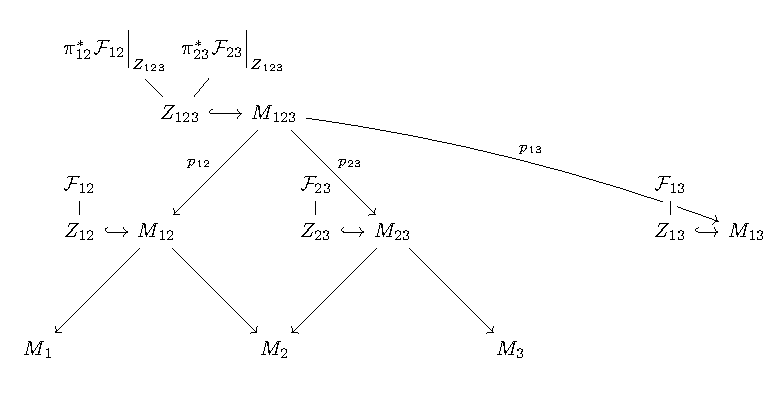
\includegraphics[]{figures/table/figure_convolution.pdf}    
    \caption{Convolution Product}  
    \label{fig:convolution_product}
\end{figure}

\section{Statement}
To facilitate the computation of intersections (i.e., tensor product in the construction of convolution product), we state the excess intersection formula.

\begin{theorem}[{Excess intersection formula, \cite[Corollary 9.4]{przezdziecki2015geometric}}]\label{thm:excess_intersection_formula}
Let $X'$ be a smooth $G$-variety, $X \subseteq X'$ be a (maybe singular) closed $G$-subvariety, and $Y_1,Y_2 \subseteq X$ be closed $G$-equivariant embeddings (of globally finite $\Tor$-dimension). Denote
\begin{equation*}
\begin{aligned}
  Y:=\;&Y_1 \cap Y_2 \qquad \iota_Y: Y \hookrightarrow X  \\
  \mathcal{T}:=\;&TX\big|_{Y} / \left( TY_1\big|_{Y}+ TY_2\big|_{Y}   \right) 
\end{aligned}
\end{equation*}
\begin{equation}\label{eq:excess_intersection_formula}
% https://q.uiver.app/?q=WzAsNyxbMSwxLCJXIl0sWzMsMSwiWiJdLFszLDIsIlgiXSxbMSwyLCJZIl0sWzQsMCwiXFxtYXRoY2Fse059X3tcXHZhcnBoaX0iXSxbMiwwLCJnXnsqfVxcbWF0aGNhbHtOfV97XFx2YXJwaGl9Il0sWzAsMCwiXFxtYXRoY2Fse059X3tcXHBoaX0iXSxbMywyLCJmIl0sWzEsMiwiXFx2YXJwaGkiXSxbMCwxLCJnIl0sWzAsMywiXFxwaGkiLDJdLFs0LDEsIiIsMCx7InN0eWxlIjp7ImhlYWQiOnsibmFtZSI6Im5vbmUifX19XSxbNSwwLCIiLDAseyJzdHlsZSI6eyJoZWFkIjp7Im5hbWUiOiJub25lIn19fV0sWzYsMCwiIiwwLHsic3R5bGUiOnsiaGVhZCI6eyJuYW1lIjoibm9uZSJ9fX1dXQ==
\begin{tikzcd}[row sep={between origins,20mm},column sep={between origins,5mm}]
	{N_Y Y_2} &[3mm]&[3mm] {\frac{N_Y X}{N_Y Y_1}} &[10mm]&[3mm] {N_{Y_1}X} \\[-9mm]
	& Y && Y_1 \\
	& Y_2 && X
	\arrow["f", from=3-2, to=3-4]
	\arrow["\varphi", from=2-4, to=3-4]
	\arrow["g", from=2-2, to=2-4]
	\arrow["\phi"', from=2-2, to=3-2]
	\arrow[no head, from=1-5, to=2-4]
	\arrow[no head, from=1-3, to=2-2]
	\arrow[no head, from=1-1, to=2-2]
\end{tikzcd}
\end{equation}
Assume that $TY_1\big|_{Y} \cap TY_2\big|_{Y} = TY$. We get the  excess intersection formula:
$$[Y_1]_{X}^G \otimes [Y_2]_{X}^G = \iota_{Y,*} \left(\eu( \mathcal{T} ) \cdot [Y]_{Y}^G \right).$$
In particular, when $Y=\pt$ is a point, we get simplified formula in $K^G(X)$:
$$[Y_1]^G \otimes [Y_2]^G = \eu( \mathcal{T} ) \cdot [Y]^G $$
where $\eu( \mathcal{T} ) \in \Rpt(G)$ acts by scalar multiplication.
\end{theorem}

Readers may find Theorem \ref{thm:excess_intersection_formula} as a special case of excess base change theorem. In fact,
\begin{equation*}
\begin{aligned}\
   [Y_1]_{X}^G \otimes [Y_2]_{X}^G=\;& [Y_1]_{X}^G \otimes f_*[Y_2]_{Y_2}^G&& \text{definition of $[Y_2]_{X}^G$}\\
   =\;& f_*\left(f^*[Y_1]_{X}^G \otimes [Y_2]_{Y_2}^G\right) && \text{proper projection formula}\\
   =\;& f_*\left(f^*[Y_1]_{X}^G \right) && \text{Lemma \ref{lem:unit_of_tensor_product}}\\
   =\;& f_*\left(f^*\varphi_{*}[Y_1]_{Y_1}^G \right) && \text{definition of $[Y_1]_{X}^G$}\\
   =\;& f_*\left(\phi_{*} \left( \eu(\mathcal{T})\cdot g^*[Y_1]_{Y_1}^G\rule{0mm}{3.6mm}  \right)\rule{0mm}{4mm} \right) && \text{excess base change to \eqref{eq:excess_intersection_formula}}\\
   =\;& \iota_{Y,*} \left(\eu( \mathcal{T} ) \cdot [Y]_{Y}^G \right) &&\\
\end{aligned}
\end{equation*}

The projection formula is stated here.
\begin{proposition}[Projection formula]
For any proper $G$-equivariant morphism $f:Y \longrightarrow X$ of globally finite $\Tor$-dimension, $\alpha \in K^G(Y)$, $\beta \in K^G(X)$, we have proper projection formula:
$$f_* \alpha \otimes \beta =f_*(\alpha \otimes f^{*} \beta).$$
\end{proposition}

\section{Application: convolution structure}
In this section, we will apply Definition \ref{def:convolution_product} and Theorem \ref{thm:excess_intersection_formula} to our typical varieties. In particular, we will get the convolution product formula in terms of basis elements $\preimage{\phi}_{\ww}$ and $\preimage{\phi}_{\ww,\ww'}$.

\subsection{Algebraic structures induced by convolution product}

\begin{defn}[Convolution product structure on $K^{G_{\dimvec{d}}}(\St_{\dimvec{d}})$]
Following notations in \ref{def:convolution_product}, We take $G=G_{\dimvec{d}}$,
\begin{equation*}
\begin{aligned}
  M_1=\;& M_2=M_3= \RRep_{\dimvec{d}}(Q) \\ 
  Z_{12}=\;& Z_{23}= \St_{\dimvec{d}} \\ 
  \St_{\dimvec{d}}=\;& \RRep_{\dimvec{d}}(Q) \times_{\Rep_{\dimvec{d}}(Q)} \RRep_{\dimvec{d}}(Q) \subseteq \RRep_{\dimvec{d}}(Q) \times \RRep_{\dimvec{d}}(Q)
\end{aligned}
\end{equation*}
By definition, we see that $\St_{\dimvec{d}} \circ \St_{\dimvec{d}} = \St_{\dimvec{d}}$. Therefore, we define a ring structure on $K^{G_{\dimvec{d}}}(\St_{\dimvec{d}})$:
$$\fakestar: K^{G_{\dimvec{d}}}(\St_{\dimvec{d}}) \times K^{G_{\dimvec{d}}}(\St_{\dimvec{d}}) \longrightarrow K^{G_{\dimvec{d}}}(\St_{\dimvec{d}}).$$
\end{defn}

\begin{defn}[$K^{G_{\dimvec{d}}}(\St_{\dimvec{d}})$-module structure on $K^{G_{\dimvec{d}}}(\RRep_{\dimvec{d}}(Q))$]
Following notations in \ref{def:convolution_product}, We take $G=G_{\dimvec{d}}$,
\begin{equation*}
\begin{aligned}
  M_1=\;& M_2= \RRep_{\dimvec{d}}(Q)  \qquad& M_3=\;& \{\pt\}\\ 
  Z_{12}=\;& \St_{\dimvec{d}} & Z_{23}=\;& \RRep_{\dimvec{d}}(Q) \\ 
\end{aligned}
\end{equation*}
By definition, we see that $\St_{\dimvec{d}} \circ \RRep_{\dimvec{d}}(Q) = \RRep_{\dimvec{d}}(Q)$. Therefore, we define a $K^{G_{\dimvec{d}}}(\St_{\dimvec{d}})$-module structure on $K^{G_{\dimvec{d}}}\left(\RRep_{\dimvec{d}}(Q)\right)$:
$$\star: K^{G_{\dimvec{d}}}(\St_{\dimvec{d}}) \times K^{G_{\dimvec{d}}}\left(\RRep_{\dimvec{d}}(Q)\right) \longrightarrow K^{G_{\dimvec{d}}}\left(\RRep_{\dimvec{d}}(Q)\right).$$
\end{defn}

\begin{remark}\label{rmk:process_convolution_product}
Notice that in the construction of the convolution product, pullback, tensor product and proper pushforward are compatible with the forgetful map of groups. Therefore, the following diagrams commute:
% https://q.uiver.app/?q=WzAsMTgsWzAsMCwiS157R197XFxkaW12ZWN7ZH19fShcXFN0X3tcXGRpbXZlY3tkfX0pIl0sWzEsMCwiS157R197XFxkaW12ZWN7ZH19fShcXFN0X3tcXGRpbXZlY3tkfX0pIl0sWzIsMCwiS157R197XFxkaW12ZWN7ZH19fShcXFN0X3tcXGRpbXZlY3tkfX0pIl0sWzMsMCwiS157R197XFxkaW12ZWN7ZH19fShcXFN0X3tcXGRpbXZlY3tkfX0pIl0sWzQsMCwiS157R197XFxkaW12ZWN7ZH19fVxcbGVmdChcXFJSZXBfe1xcZGltdmVje2R9fShRKVxccmlnaHQpIl0sWzUsMCwiS157R197XFxkaW12ZWN7ZH19fVxcbGVmdChcXFJSZXBfe1xcZGltdmVje2R9fShRKVxccmlnaHQpIl0sWzAsMSwiS157VF97XFxkaW12ZWN7ZH19fShcXFN0X3tcXGRpbXZlY3tkfX0pIl0sWzEsMSwiS157VF97XFxkaW12ZWN7ZH19fShcXFN0X3tcXGRpbXZlY3tkfX0pIl0sWzIsMSwiS157VF97XFxkaW12ZWN7ZH19fShcXFN0X3tcXGRpbXZlY3tkfX0pIl0sWzMsMSwiS157VF97XFxkaW12ZWN7ZH19fShcXFN0X3tcXGRpbXZlY3tkfX0pIl0sWzQsMSwiS157VF97XFxkaW12ZWN7ZH19fVxcbGVmdChcXFJSZXBfe1xcZGltdmVje2R9fShRKVxccmlnaHQpIl0sWzUsMSwiS157VF97XFxkaW12ZWN7ZH19fVxcbGVmdChcXFJSZXBfe1xcZGltdmVje2R9fShRKVxccmlnaHQpIl0sWzAsMiwiXFxLY3VybF57VF97XFxkaW12ZWN7ZH19fShcXFN0X3tcXGRpbXZlY3tkfX0pIl0sWzEsMiwiXFxLY3VybF57VF97XFxkaW12ZWN7ZH19fShcXFN0X3tcXGRpbXZlY3tkfX0pIl0sWzIsMiwiXFxLY3VybF57VF97XFxkaW12ZWN7ZH19fShcXFN0X3tcXGRpbXZlY3tkfX0pIl0sWzMsMiwiXFxLY3VybF57VF97XFxkaW12ZWN7ZH19fShcXFN0X3tcXGRpbXZlY3tkfX0pIl0sWzQsMiwiXFxLY3VybF57VF97XFxkaW12ZWN7ZH19fVxcbGVmdChcXFJSZXBfe1xcZGltdmVje2R9fShRKVxccmlnaHQpIl0sWzUsMiwiXFxLY3VybF57VF97XFxkaW12ZWN7ZH19fVxcbGVmdChcXFJSZXBfe1xcZGltdmVje2R9fShRKVxccmlnaHQpIl0sWzAsNiwiIiwwLHsic3R5bGUiOnsidGFpbCI6eyJuYW1lIjoiaG9vayIsInNpZGUiOiJib3R0b20ifX19XSxbMSw3LCIiLDAseyJzdHlsZSI6eyJ0YWlsIjp7Im5hbWUiOiJob29rIiwic2lkZSI6ImJvdHRvbSJ9fX1dLFsyLDgsIiIsMCx7InN0eWxlIjp7InRhaWwiOnsibmFtZSI6Imhvb2siLCJzaWRlIjoiYm90dG9tIn19fV0sWzMsOSwiIiwwLHsic3R5bGUiOnsidGFpbCI6eyJuYW1lIjoiaG9vayIsInNpZGUiOiJib3R0b20ifX19XSxbNCwxMCwiIiwwLHsic3R5bGUiOnsidGFpbCI6eyJuYW1lIjoiaG9vayIsInNpZGUiOiJib3R0b20ifX19XSxbNiwxMiwiIiwwLHsic3R5bGUiOnsidGFpbCI6eyJuYW1lIjoiaG9vayIsInNpZGUiOiJib3R0b20ifX19XSxbNywxMywiIiwwLHsic3R5bGUiOnsidGFpbCI6eyJuYW1lIjoiaG9vayIsInNpZGUiOiJib3R0b20ifX19XSxbOCwxNCwiIiwwLHsic3R5bGUiOnsidGFpbCI6eyJuYW1lIjoiaG9vayIsInNpZGUiOiJib3R0b20ifX19XSxbOSwxNSwiIiwwLHsic3R5bGUiOnsidGFpbCI6eyJuYW1lIjoiaG9vayIsInNpZGUiOiJib3R0b20ifX19XSxbMTAsMTYsIiIsMCx7InN0eWxlIjp7InRhaWwiOnsibmFtZSI6Imhvb2siLCJzaWRlIjoiYm90dG9tIn19fV0sWzUsMTEsIiIsMCx7InN0eWxlIjp7InRhaWwiOnsibmFtZSI6Imhvb2siLCJzaWRlIjoiYm90dG9tIn19fV0sWzExLDE3LCIiLDAseyJzdHlsZSI6eyJ0YWlsIjp7Im5hbWUiOiJob29rIiwic2lkZSI6ImJvdHRvbSJ9fX1dLFs0LDUsIlxcZGl2aWRlb250aW1lcyJdLFsxMCwxMSwiXFxkaXZpZGVvbnRpbWVzIl0sWzE2LDE3LCJcXGRpdmlkZW9udGltZXMiXSxbMSwyLCIqIl0sWzcsOCwiKiJdLFsxMywxNCwiKiJdLFszLDQsIlxcdGltZXMiLDEseyJzdHlsZSI6eyJib2R5Ijp7Im5hbWUiOiJub25lIn0sImhlYWQiOnsibmFtZSI6Im5vbmUifX19XSxbOSwxMCwiXFx0aW1lcyIsMSx7InN0eWxlIjp7ImJvZHkiOnsibmFtZSI6Im5vbmUifSwiaGVhZCI6eyJuYW1lIjoibm9uZSJ9fX1dLFsxNSwxNiwiXFx0aW1lcyIsMSx7InN0eWxlIjp7ImJvZHkiOnsibmFtZSI6Im5vbmUifSwiaGVhZCI6eyJuYW1lIjoibm9uZSJ9fX1dLFswLDEsIlxcdGltZXMiLDEseyJzdHlsZSI6eyJib2R5Ijp7Im5hbWUiOiJub25lIn0sImhlYWQiOnsibmFtZSI6Im5vbmUifX19XSxbNiw3LCJcXHRpbWVzIiwxLHsic3R5bGUiOnsiYm9keSI6eyJuYW1lIjoibm9uZSJ9LCJoZWFkIjp7Im5hbWUiOiJub25lIn19fV0sWzEyLDEzLCJcXHRpbWVzIiwxLHsic3R5bGUiOnsiYm9keSI6eyJuYW1lIjoibm9uZSJ9LCJoZWFkIjp7Im5hbWUiOiJub25lIn19fV1d
\[\begin{tikzcd}
	{K^{G_{\dimvec{d}}}(\St_{\dimvec{d}})} &[-9mm] {K^{G_{\dimvec{d}}}(\St_{\dimvec{d}})} &[-3mm] {K^{G_{\dimvec{d}}}(\St_{\dimvec{d}})} &[-3mm] {K^{G_{\dimvec{d}}}(\St_{\dimvec{d}})} &[-9mm] {K^{G_{\dimvec{d}}}\left(\RRep_{\dimvec{d}}(Q)\right)} &[-3mm] {K^{G_{\dimvec{d}}}\left(\RRep_{\dimvec{d}}(Q)\right)} \\
	{K^{T_{\dimvec{d}}}(\St_{\dimvec{d}})} & {K^{T_{\dimvec{d}}}(\St_{\dimvec{d}})} & {K^{T_{\dimvec{d}}}(\St_{\dimvec{d}})} & {K^{T_{\dimvec{d}}}(\St_{\dimvec{d}})} & {K^{T_{\dimvec{d}}}\left(\RRep_{\dimvec{d}}(Q)\right)} & {K^{T_{\dimvec{d}}}\left(\RRep_{\dimvec{d}}(Q)\right)} \\
	{\Kcurl^{T_{\dimvec{d}}}(\St_{\dimvec{d}})} & {\Kcurl^{T_{\dimvec{d}}}(\St_{\dimvec{d}})} & {\Kcurl^{T_{\dimvec{d}}}(\St_{\dimvec{d}})} & {\Kcurl^{T_{\dimvec{d}}}(\St_{\dimvec{d}})} & {\Kcurl^{T_{\dimvec{d}}}\left(\RRep_{\dimvec{d}}(Q)\right)} & {\Kcurl^{T_{\dimvec{d}}}\left(\RRep_{\dimvec{d}}(Q)\right)}
	\arrow[hook', from=1-1, to=2-1]
	\arrow[hook', from=1-2, to=2-2]
	\arrow[hook', from=1-3, to=2-3]
	\arrow[hook', from=1-4, to=2-4]
	\arrow[hook', from=1-5, to=2-5]
	\arrow[hook', from=2-1, to=3-1]
	\arrow[hook', from=2-2, to=3-2]
	\arrow[hook', from=2-3, to=3-3]
	\arrow[hook', from=2-4, to=3-4]
	\arrow[hook', from=2-5, to=3-5]
	\arrow[hook', from=1-6, to=2-6]
	\arrow[hook', from=2-6, to=3-6]
	\arrow["\star", from=1-5, to=1-6]
	\arrow["\star", from=2-5, to=2-6]
	\arrow["\star", from=3-5, to=3-6]
	\arrow["\fakestar", from=1-2, to=1-3]
	\arrow["\fakestar", from=2-2, to=2-3]
	\arrow["\fakestar", from=3-2, to=3-3]
	\arrow["\times"{description}, draw=none, from=1-4, to=1-5]
	\arrow["\times"{description}, draw=none, from=2-4, to=2-5]
	\arrow["\times"{description}, draw=none, from=3-4, to=3-5]
	\arrow["\times"{description}, draw=none, from=1-1, to=1-2]
	\arrow["\times"{description}, draw=none, from=2-1, to=2-2]
	\arrow["\times"{description}, draw=none, from=3-1, to=3-2]
\end{tikzcd}\]
\end{remark}

\begin{defn}[$K^{G_{\dimvec{d}}}(\RRep_{\dimvec{d}}(Q))$-module structure on $K^{G_{\dimvec{d}}}(\St_{\dimvec{d}})$]
We know that 
$$\RRep_{\dimvec{d}}(Q) \cong \St_{\Id} \subseteq \St_{\dimvec{d}}, \qquad \St_{\Id} \circ \St_{\Id} = \St_{\Id},$$
so $K^{G_{\dimvec{d}}}\left(\RRep_{\dimvec{d}}(Q)\right)$ can be realized as a $R(G_{\dimvec{d}})$-subalgebra of $K^{G_{\dimvec{d}}}(\St_{\dimvec{d}})$, and $K^{G_{\dimvec{d}}}(\St_{\dimvec{d}})$ has the $K^{G_{\dimvec{d}}}\left(\RRep_{\dimvec{d}}(Q)\right)$-module structure induced by the convolution product:
$$\fakestar: K^{G_{\dimvec{d}}}\left(\RRep_{\dimvec{d}}(Q)\right) \times K^{G_{\dimvec{d}}}(\St_{\dimvec{d}}) \longrightarrow K^{G_{\dimvec{d}}}(\St_{\dimvec{d}}).$$
\end{defn}

\subsection{Convolution product formula}\label{subsec:convolution_product_fml}


In this subsection, we compute the convolution product in the bottom line of the diagram in Remark \ref{rmk:process_convolution_product}.
\begin{proposition}[Convolution product formula]\label{prop:convolution_product_formula}
For $\ww$, $\ww'$, $\ww''$, $\ww''' \in \WWd$, we have
\begin{equation*}
\begin{aligned}
  \preimage{\psi}_{\ww,\ww'} \fakestar \preimage{\psi}_{\ww'',\ww'''}=\;& \delta_{\ww',\ww''}\preimage{\Lambda}_{\ww'} \preimage{\psi}_{\ww,\ww'''} \\ 
  \preimage{\psi}_{\ww,\ww'} \star \preimage{\psi}_{\ww''\phantom{,\ww'''}}=\;& \delta_{\ww',\ww''}\preimage{\Lambda}_{\ww'} \preimage{\psi}_{\ww}. \\   
\end{aligned}
\end{equation*}
\end{proposition}
\begin{proof}
Follow the Definition \ref{def:convolution_product} and Theorem \ref{thm:excess_intersection_formula} if needed.

For clearance, we divide the proof into four cases.

\paragraph*{\underline{Case 1.}}Assume $\ww' \neq \ww''$, need to show $\preimage{\psi}_{\ww,\ww'} \fakestar \preimage{\psi}_{\ww'',\ww'''}=0$.\\[-3mm]

Denote 
%\footnote{For some people, the notation
%$$Y_{12}:= \left\{\rule{0mm}{3mm}\!\left(\rule{0mm}{2.8mm}(\rho_0, F_{\ww}),(\rho_0, F_{\ww'})\right) \right\} \subseteq \St_{\dimvec{d}}$$ is better for understanding. We don't write like that, because too many brackets occupy attentions.
%}
$$Y_{12}:= \{(\rho_0, F_{\ww}, F_{\ww'}) \} \subseteq \St_{\dimvec{d}}, \qquad Y_{23}:= \{(\rho_0, F_{\ww''}, F_{\ww'''}) \} \subseteq \St_{\dimvec{d}}.$$
Since $\ww' \neq \ww''$, $p_{12}^{-1} (Y_{12}) \cap
p_{23}^{-1} (Y_{23}) = \varnothing$, so
\begin{equation*}
\begin{aligned}
\preimage{\psi}_{\ww,\ww'} \fakestar \preimage{\psi}_{\ww'',\ww'''}=\;& \left[ Y_{12}   \right]_{\St_{\dimvec{d}}}^{T_{\dimvec{d}}}  \fakestar \left[ Y_{23}  \right]_{\St_{\dimvec{d}}}^{T_{\dimvec{d}}}\\ 
=\;&p_{13,*}\left(p_{12}^* \left[ Y_{12}   \right]_{M_{12}}^{T_{\dimvec{d}}}  \otimes p_{23}^* \left[ Y_{23}  \right]_{M_{23}}^{T_{\dimvec{d}}} \right)\\
=\;&p_{13,*}\left(\left[ p_{12}^{-1}(Y_{12})   \right]_{M_{123}}^{T_{\dimvec{d}}}  \otimes \left[  p_{12}^{-1}(Y_{23})  \right]_{M_{123}}^{T_{\dimvec{d}}} \right)\\
=\;&0
\end{aligned}
\end{equation*}

\paragraph*{\underline{Case 2.}}Assume $\ww' \neq \ww''$, need to show $\preimage{\psi}_{\ww,\ww'} \star \preimage{\psi}_{\ww''}=0$.\\[-3mm]

Denote
$$Y_{12}:= \{(\rho_0, F_{\ww}, F_{\ww'}) \} \subseteq \St_{\dimvec{d}}, \qquad Y_{23}:= \{(\rho_0, F_{\ww''}) \} \subseteq \RRep_{\dimvec{d}}(Q).$$
Since $\ww' \neq \ww''$, $p_{12}^{-1} (Y_{12}) \cap
p_{23}^{-1} (Y_{23}) = \varnothing$, so
\begin{equation*}
\begin{aligned}
\preimage{\psi}_{\ww,\ww'} \star \preimage{\psi}_{\ww''}=\;& \left[ Y_{12}   \right]_{\St_{\dimvec{d}}}^{T_{\dimvec{d}}}  \star \left[ Y_{23}  \right]_{\RRep_{\dimvec{d}}(Q)}^{T_{\dimvec{d}}}\\ 
=\;&p_{13,*}\left(p_{12}^* \left[ Y_{12}   \right]_{M_{12}}^{T_{\dimvec{d}}}  \otimes p_{23}^* \left[ Y_{23}  \right]_{M_{23}}^{T_{\dimvec{d}}} \right)\\
=\;&p_{13,*}\left(\left[ p_{12}^{-1}(Y_{12})   \right]_{M_{123}}^{T_{\dimvec{d}}}  \otimes \left[  p_{12}^{-1}(Y_{23})  \right]_{M_{123}}^{T_{\dimvec{d}}} \right)\\
=\;&0
\end{aligned}
\end{equation*}

\paragraph*{\underline{Case 3.}}For $\ww$, $\ww'$, $\ww'' \in \WWd$, need to show that $$\preimage{\psi}_{\ww,\ww'} \fakestar \preimage{\psi}_{\ww',\ww''}=\preimage{\Lambda}_{\ww'}\preimage{\psi}_{\ww,\ww''}.$$

Denote 
$$Y_{12}:= \{(\rho_0, F_{\ww}, F_{\ww'}) \} \subseteq \St_{\dimvec{d}}, \qquad Y_{23}:= \{(\rho_0, F_{\ww'}, F_{\ww''}) \} \subseteq \St_{\dimvec{d}},$$
then
\begin{equation*}
\begin{aligned}
  &p_{12}^{-1}(Y_{12})= Y_{12} \times \RRep_{\dimvec{d}}(Q) \qquad & p_{23}^{-1}(Y_{23})=\;&   \RRep_{\dimvec{d}}(Q) \times Y_{23}\\ 
  &p_{12}^{-1}(Y_{12}) \cup p_{23}^{-1}(Y_{23})=Y & Y_{12}\circ Y_{23}=\;&Y_{13},
\end{aligned}
\end{equation*}
where
\begin{equation*}
\begin{aligned}
  &Y=\{y\} \qquad && y=\big( (\rho_0,F_{\ww}),(\rho_0,F_{\ww'}),(\rho_0,F_{\ww''})  \big) & &\in M_{123}  \\ 
  &Y_{13}=\{y_{13}\} \qquad && y_{13}=\big( (\rho_0,F_{\ww}),(\rho_0,F_{\ww''})  \big) & &\in M_{13}  \\
\end{aligned}
\end{equation*}
Therefore, 
\begin{equation*}
\begin{aligned}
\preimage{\psi}_{\ww,\ww'} \fakestar \preimage{\psi}_{\ww',\ww''}=\;& \left[ Y_{12}   \right]_{\St_{\dimvec{d}}}^{T_{\dimvec{d}}}  \fakestar \left[ Y_{23}  \right]_{\St_{\dimvec{d}}}^{T_{\dimvec{d}}}\\ 
=\;&p_{13,*}\left(p_{12}^* \left[ Y_{12}   \right]_{M_{12}}^{T_{\dimvec{d}}}  \otimes p_{23}^* \left[ Y_{23}  \right]_{M_{23}}^{T_{\dimvec{d}}} \right)\\
=\;&p_{13,*}\left(\left[ p_{12}^{-1}(Y_{12})   \right]_{M_{123}}^{T_{\dimvec{d}}}  \otimes \left[  p_{12}^{-1}(Y_{23})  \right]_{M_{123}}^{T_{\dimvec{d}}} \right)\\
=\;&p_{13,*}\left(\eu( \mathcal{T} ) \cdot [Y]_{M_{123}}^{T_{\dimvec{d}}} \right)\\
=\;&\eu( \mathcal{T} )\cdot [Y]_{M_{13}}^{T_{\dimvec{d}}} \\
=\;& \preimage{\Lambda}_{\ww'}\preimage{\psi}_{\ww,\ww''}
\end{aligned}
\end{equation*}
where
$$\mathcal{T}:= \frac{T_y M_{123} }{T_y \big( p_{12}^{-1}(Y_{12}) \big) \oplus T_y \big( p_{23}^{-1}(Y_{23}) \big)} = \frac{\preimage{\mathcal{T}}_{\ww} \oplus \preimage{\mathcal{T}}_{\ww'} \oplus \preimage{\mathcal{T}}_{\ww''}}{\preimage{\mathcal{T}}_{\ww} \hfill\oplus \hfill  \preimage{\mathcal{T}}_{\ww''}}= \preimage{\mathcal{T}}_{\ww'}.$$
\paragraph*{\underline{Case 4.}}For $\ww$, $\ww' \in \WWd$, need to show that $$\preimage{\psi}_{\ww,\ww'} \star \preimage{\psi}_{\ww'}=\preimage{\Lambda}_{\ww'}\preimage{\psi}_{\ww}.$$

Denote 
$$Y_{12}:= \{(\rho_0, F_{\ww}, F_{\ww'}) \} \subseteq \St_{\dimvec{d}}, \qquad Y_{23}:= \{(\rho_0, F_{\ww'}) \} \subseteq \RRep_{\dimvec{d}}(Q),$$
then
\begin{equation*}
\begin{aligned}
  &p_{12}^{-1}(Y_{12})= Y_{12} \times \{\pt\} \qquad & p_{23}^{-1}(Y_{23})=\;&   \RRep_{\dimvec{d}}(Q) \times Y_{23}\\ 
  &p_{12}^{-1}(Y_{12}) \cup p_{23}^{-1}(Y_{23})=Y \qquad& Y_{12}\circ Y_{23}=\;&Y_{13},
\end{aligned}
\end{equation*}
where
\begin{equation*}
\begin{aligned}
  &Y=\{y\} \qquad && y=\big( (\rho_0,F_{\ww}),(\rho_0,F_{\ww'})  \big) & &\in M_{123}  \\ 
  &Y_{13}=\{y_{13}\} \qquad && y_{13}= (\rho_0,F_{\ww}) & &\in M_{13}  \\
\end{aligned}
\end{equation*}
Therefore, 
\begin{equation*}
\begin{aligned}
\preimage{\psi}_{\ww,\ww'} \star \preimage{\psi}_{\ww'}=\;& \left[ Y_{12}   \right]_{\St_{\dimvec{d}}}^{T_{\dimvec{d}}}  \star \left[ Y_{23}  \right]_{\RRep_{\dimvec{d}}(Q)}^{T_{\dimvec{d}}}\\ 
=\;&p_{13,*}\left(p_{12}^* \left[ Y_{12}   \right]_{M_{12}}^{T_{\dimvec{d}}}  \otimes p_{23}^* \left[ Y_{23}  \right]_{M_{23}}^{T_{\dimvec{d}}} \right)\\
=\;&p_{13,*}\left(\left[ p_{12}^{-1}(Y_{12})   \right]_{M_{123}}^{T_{\dimvec{d}}}  \otimes \left[  p_{12}^{-1}(Y_{23})  \right]_{M_{123}}^{T_{\dimvec{d}}} \right)\\
=\;&p_{13,*}\left(\eu( \mathcal{T} ) \cdot [Y]_{M_{123}}^{T_{\dimvec{d}}} \right)\\
=\;&\eu( \mathcal{T} )\cdot [Y]_{M_{13}}^{T_{\dimvec{d}}} \\
=\;& \preimage{\Lambda}_{\ww'}\preimage{\psi}_{\ww}
\end{aligned}
\end{equation*}
where
$$\mathcal{T}:= \frac{T_y M_{123} }{T_y \big( p_{12}^{-1}(Y_{12}) \big) \oplus T_y \big( p_{23}^{-1}(Y_{23}) \big)} = \frac{\preimage{\mathcal{T}}_{\ww} \oplus \preimage{\mathcal{T}}_{\ww'} \oplus 0}{\preimage{\mathcal{T}}_{\ww} \hfill\oplus \hfill  0}= \preimage{\mathcal{T}}_{\ww'}.$$

\end{proof}


\subsection{Demazure operator}
In this subsection, we will compute the action of some elements in $K^{G_{\dimvec{d}}}  (\St_{\ftdimvec{d},\ftdimvec{d}'})$ acting on $K^{G_{\dimvec{d}}} \left( \RRep_{\ftdimvec{d}'}(Q) \right)$. As a reminder,
% https://q.uiver.app/?q=WzAsNCxbMCwwLCJLXntHX3tcXGRpbXZlY3tkfX19IFxcbGVmdCggXFxSUmVwX3tcXGZ0ZGltdmVje2R9J30oUSkgXFxyaWdodCkiXSxbMCwxLCJLXntUX3tcXGRpbXZlY3tkfX19IFxcbGVmdCggXFxSUmVwX3tcXGZ0ZGltdmVje2R9J30oUSkgXFxyaWdodCkiXSxbMSwxLCJcXGRpc3BsYXlzdHlsZVxcYmlnb3BsdXNfe3d9IFxcUnB0KFRfe1xcZGltdmVje2R9fSkgXFxsZWZ0WyBcXG92ZXJsaW5le1xccHJlaW1hZ2V7XFxPbWNlbGx9fV97d31ee3V9IFxccmlnaHRdXntUX3tcXGRpbXZlY3tkfX19Il0sWzEsMCwiXFxkaXNwbGF5c3R5bGVcXHBoYW50b217XFxiaWdvcGx1c197d319XFxScHQoVF97XFxkaW12ZWN7ZH19KSBcXGxlZnRbIFxcUlJlcF97XFxmdGRpbXZlY3tkfSd9KFEpIFxccmlnaHRdXntHX3tcXGRpbXZlY3tkfX19Il0sWzMsMl0sWzAsMV0sWzAsMywiXFxjb25nIiwxLHsic3R5bGUiOnsiYm9keSI6eyJuYW1lIjoibm9uZSJ9LCJoZWFkIjp7Im5hbWUiOiJub25lIn19fV0sWzEsMiwiXFxjb25nIiwxLHsic3R5bGUiOnsiYm9keSI6eyJuYW1lIjoibm9uZSJ9LCJoZWFkIjp7Im5hbWUiOiJub25lIn19fV1d
\begin{equation}\label{eq:shift_G_T}
\begin{tikzcd}[column sep={between origins, 38mm}, row sep={between origins, 18mm}]
	{K^{G_{\dimvec{d}}} \left( \RRep_{\ftdimvec{d}'}(Q) \right)} & {\displaystyle\phantom{\bigoplus_{w}}\Rpt(T_{\dimvec{d}}) \left[ \RRep_{\ftdimvec{d}'}(Q) \right]^{G_{\dimvec{d}}}\hspace{-10mm}} \\
	{K^{T_{\dimvec{d}}} \left( \RRep_{\ftdimvec{d}'}(Q) \right)} & {\displaystyle\bigoplus_{w} \Rpt(T_{\dimvec{d}}) \left[ \overline{\preimage{\Omcell}}_{w}^{u} \right]^{T_{\dimvec{d}}}}
	\arrow[from=1-2, to=2-2]
	\arrow[from=1-1, to=2-1]
	\arrow["\cong"{description}, draw=none, from=1-1, to=1-2]
	\arrow["\cong"{description}, draw=none, from=2-1, to=2-2]
\end{tikzcd}
\end{equation}
where the $R(T_{\dimvec{d}})$-module structure on $K^{G_{\dimvec{d}}} \left( \RRep_{\ftdimvec{d}'}(Q) \right)$ is induced by the induction formula.

For $f \in \Rpt(T_{\dimvec{d}}) \cong \mathbb{Z}\!\left[ e_1^{\pm 1},\ldots,e_{\abdimvec{d}}^{\pm 1} \right]$, denote $f^{u}:=f \cdot \left[ \RRep_{\ftdimvec{d}'}(Q) \right]^{G_{\dimvec{d}}}$. Under the morphism \eqref{eq:shift_G_T}, $f$ is sent to $f \cdot \left[ \RRep_{\ftdimvec{d}'}(Q) \right]^{T_{\dimvec{d}}}$. Viewing $f^{u}$ as an element in $\Kcurl^{G_{\dimvec{d}}} \left( \RRep_{\ftdimvec{d}'}(Q) \right)$, we get
$$f^{u}=\sum_{w} f(e_1,\ldots,e_{\abdimvec{d}}) \preimage{\Lambda}_{wu}^{-1} \preimage{\psi}_{wu}.$$
\begin{remark}\label{rmk:relabling_of_coef}
This formula looks not so compatible with the group action. To facilitate our computation, we relable the coefficient ring before $\preimage{\psi}_{\ww}$ by $e_i^{\ww}:= e_{\ww^{-1}(i)}$, which means that
$$K^{T_{\dimvec{d}}} \left(\RRep_{\dimvec{d}}(Q)\right) \cong \bigoplus_{\ww} \mathbb{Z}\!\left[ e_1^{\ww,\pm 1},\ldots,e_{\abdimvec{d}}^{\ww,\pm 1} \right] \preimage{\psi}_{\ww}$$
Therefore, 
\begin{equation*}
\begin{aligned}
 f^{u} =\;&  \sum_{w} (wuf)(e_1^{wu},\ldots,e_{\abdimvec{d}}^{wu}) \preimage{\Lambda}_{wu}^{-1} \preimage{\psi}_{wu}.\\ 
 \hat{=}\;&  \sum_{w} (wuf) \; \preimage{\Lambda}_{wu}^{-1} \preimage{\psi}_{wu}.\\ 
\end{aligned}
\end{equation*}
Later, every expression before $\preimage{\psi}_{\ww}$ should be viewed as an expression in $\mathbb{Z}\!\left[ e_1^{\ww,\pm 1},\ldots,e_{\abdimvec{d}}^{\ww,\pm 1} \right]$.
\end{remark}

\begin{defn}[Demazure operator]
For $i \in \{ 1,\ldots, \abdimvec{d}-1 \}$, set $s=s_i$, the (absolute) Demazure operator is defined as
$$D_i:= \left[\St_{s_i} \right]^{G_{\dimvec{d}}} \in K^{G_{\dimvec{d}}}(\St_{\dimvec{d}}).$$
View $D_i$ as an element in $\Kcurl^{T_{\dimvec{d}}}(\St_{\dimvec{d}})$, we get
$$D_i=\sum_{\ww \in \WWd} \left( \preimage{\Lambda}_{\ww,\ww s}^{s} \right)^{-1} \preimage{\psi}_{\ww,\ww s} + \sum_{\stackrel{\ww \in \WWd}{\ww s \ww^{-1}\in \Wd}} \left( \preimage{\Lambda}_{\ww,\ww}^{s} \right)^{-1} \preimage{\psi}_{\ww,\ww}.$$

We also have the relative version. Suppose that $\Wd us_i=\Wd u'$ (which guarantees the existence of $\St_{s_i}^{u,u'}$), the (relative) Demazure operator is defined as
$$D_i^{u,u'}:= \left[\St_{s_i}^{u,u'} \right]^{G_{\dimvec{d}}} \in K^{G_{\dimvec{d}}}(\St^{u,u'}).$$
View $D_i^{u,u'}$ as an element in $\Kcurl^{T_{\dimvec{d}}}(\St^{u,u'})$, we get
$$D_i^{u,u'}=\sum_{w} \left( \preimage{\Lambda}_{wu,wu s}^{s} \right)^{-1} \preimage{\psi}_{wu,wu s} + \delta_{u,u'}\sum_{w} \left( \preimage{\Lambda}_{wu,wu}^{s} \right)^{-1} \preimage{\psi}_{wu,wu}.$$

The equivariant cohomology theory version of Demazure operators are denoted by $\partial_i$ and $\partial_i^{u,u'}$.
\end{defn}
\begin{theorem}\label{thm:Demazure_operator_1}
We obtain a formula for the Demazure operator:
\begin{equation*}\label{eq:Demazure_operator}
D_i^{u,u'} \star f^{u'}=\begin{cases}
\left[\left( \raisebox{1mm}{$\displaystyle\frac{s_i f}{ 1-\frac{e_{i+1}}{e_{i}}}     + \frac{f}{1-\frac{e_{i}}{e_{i+1}}}$}  \right)\left(\displaystyle 1-\frac{e_{i+1}}{e_{i}}\right)^{k} \right]^{u} & u=u',\\[8mm]
\left[s_i f  \left(\displaystyle 1-\frac{e_{i+1}}{e_{i}}\right)^{k} \right]^{u} & u \neq u'.
\end{cases}
\end{equation*}
and similarly in equivariant cohomology:
\begin{equation*}\label{eq:Demazure_operator_cth}
\partial_i^{u,u'} \star f^{u'}=\begin{cases}
\left[\left( \displaystyle\frac{s_i f}{ \lambda_{i+1}-\lambda_{i}}     + \frac{f}{\lambda_{i}-\lambda_{i+1} }  \right)\left(\lambda_{i+1}-\lambda_{i}\right)^{k} \right]^{u} & u=u',\\[8mm]
\left[s_i f  \left(\lambda_{i+1}-\lambda_{i}\right)^{k} \right]^{u} & u \neq u'.
\end{cases}
\end{equation*}
In the formula, $\lambda_l^{u}:=\lambda_{u^{-1}(l)}$, and $k$ stands for the number of arrows from the vertex associated to $v_{u(i+1)}$ to the vertex associated to $v_{u(i)}$.
\end{theorem}

In the computation we mainly focus on the $K$-theory case. Using \ref{rmk:relabling_of_coef}, one can compute $D_i^{u,u'} \star f^{u'}$ in terms of $\phi$'s: ($s:=s_i$ for simplicity)
\begingroup
%\allowdisplaybreaks
\begin{align*}
  D_i^{u,u'} \star f^{u'}=\;& \left(\sum_{w} \left( \preimage{\Lambda}_{wu,wu s}^{s} \right)^{-1} \preimage{\psi}_{wu,wu s} + \delta_{u,u'}\sum_{w} \left( \preimage{\Lambda}_{wu,wu}^{s} \right)^{-1} \preimage{\psi}_{wu,wu}\right) \\ 
  &\hspace{70mm}\star \left(\sum_{w} (wu'f) \; \preimage{\Lambda}_{wu'}^{-1} \preimage{\psi}_{wu'}\right)\\
  =\;& \left(\sum_{w} \left( \preimage{\Lambda}_{wu,wu s}^{s} \right)^{-1} \preimage{\psi}_{wu,wu s}\right) \star \left(\sum_{w} (wusf) \; \preimage{\Lambda}_{wus}^{-1} \preimage{\psi}_{wus}\right)\\
  & +\delta_{u,u'}\left(\sum_{w} \left( \preimage{\Lambda}_{wu,wu}^{s} \right)^{-1} \preimage{\psi}_{wu,wu}\right) \star \left(\sum_{w} (wuf) \; \preimage{\Lambda}_{wu}^{-1} \preimage{\psi}_{wu}\right)\\
  =\;& \left(\sum_{w} (wusf) \left( \preimage{\Lambda}_{wu,wu s}^{s} \right)^{-1} \preimage{\psi}_{wu} \right) +\delta_{u,u'}\left(\sum_{w} (wuf) \left( \preimage{\Lambda}_{wu,wu}^{s} \right)^{-1} \preimage{\psi}_{wu} \right)\\
  =\;& \sum_{w}
  \left[ \left(\frac{wusf}{\preimage{\Lambda}_{wu,wu s}^{s}}     +\delta_{u,u'} \frac{wuf}{\preimage{\Lambda}_{wu,wu}^{s}} \right) \preimage{\Lambda}_{wu} \right]\preimage{\Lambda}_{wu}^{-1}\preimage{\psi}_{wu} \\
  =\;& \sum_{w} w
  \left[  \left(\frac{usf}{\preimage{\Lambda}_{u,u s}^{s}}     +\delta_{u,u'} \frac{uf}{\preimage{\Lambda}_{u,u}^{s}} \right) \preimage{\Lambda}_{u} \right]\preimage{\Lambda}_{wu}^{-1}\preimage{\psi}_{wu} \\
  =\;& \sum_{w} wu
    \left[  \left(\frac{sf}{u^{-1}\preimage{\Lambda}_{u,u s}^{s}}     +\delta_{u,u'} \frac{f}{u^{-1}\preimage{\Lambda}_{u,u}^{s}} \right) u^{-1}\preimage{\Lambda}_{u} \right]\preimage{\Lambda}_{wu}^{-1}\preimage{\psi}_{wu} \\
  =\;& 
        \left[  \left(\frac{sf}{u^{-1}\preimage{\Lambda}_{u,u s}^{s}}     +\delta_{u,u'} \frac{f}{u^{-1}\preimage{\Lambda}_{u,u}^{s}} \right) u^{-1}\preimage{\Lambda}_{u} \right]^{u}    
\end{align*}
\endgroup
Recall Subsection \ref{subsec:tangent_space} (especially Proposition  \ref{prop:tangent_space_2}), we get
$$
\preimage{\mathcal{T}}_{u,us}^{s}\cong \mathfrak{r}_{u,us} \oplus \mathfrak{n}_{u}^{-} \oplus \mathfrak{m}_{u,us}
\qquad
\preimage{\mathcal{T}}_{u,u}^{s}\cong  \mathfrak{r}_{u,us} \oplus \mathfrak{n}_{u}^{-} \oplus \mathfrak{m}_{us,u}
\qquad
\preimage{\mathcal{T}}_{u} \cong \mathfrak{r}_{u} \oplus \mathfrak{n}_{u}^{-}. $$
Therefore, 
\begin{equation}\label{eq:final_destination}
D_i^{u,u'} \star f^{u'}=\left[\left(\frac{sf}{u^{-1}\eu(\mathfrak{m}_{u,us})}     +\delta_{u,u'} \frac{f}{u^{-1}\eu(\mathfrak{m}_{us,u})}  \right)u^{-1}\eu(\mathfrak{d}_{u,us}) \right]^{u}.
\end{equation}
Recall the computation in \ref{eg:5-case-3} and Section \ref{sec:euler_class}. We collect needed information in Table \ref{table:euler_class_1}.

\begin{table}[ht]
  \vspace{0cm}
    \centering  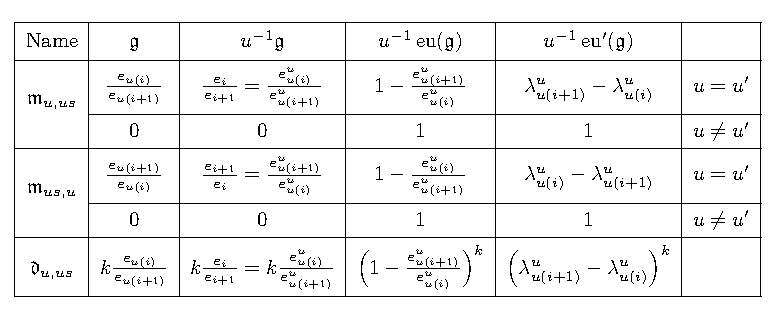
\includegraphics[width=12cm]{figures/table/table_euler_class.pdf}
      \caption{}
      \label{table:euler_class_1}        
\end{table}

Theorem \ref{thm:Demazure_operator_1} is our final destination in this part. We will express its importance in Subsection \ref{subsec:miscellaneous}, see some generalizations in Section \ref{sec:generalization} and compute some examples in Section \ref{sec:diagram}.

\subsection{Miscellaneous}\label{subsec:miscellaneous}
In this subsection, we collect some more results. The arguments in reference work for both $K$-theory and cohomology theory.

\begin{proposition}\label{prop:faithfulness}
The action of $K^{G_{\dimvec{d}}}(\St_{\dimvec{d}})$ on $K^{G_{\dimvec{d}}}(\RRep_{\dimvec{d}}(Q))$ is faithful.
\end{proposition}
\begin{proof}[Sketch of proof]
Reduce the problem to the faithfulness for the action of $\Kcurl^{T_{\dimvec{d}}}(\St_{\dimvec{d}})$ on $\Kcurl^{T_{\dimvec{d}}}(\RRep_{\dimvec{d}}(Q))$. For details, see \cite[Theorem 10.10]{przezdziecki2015geometric}.
\end{proof}

\begin{proposition}\label{prop:generators}
The elements $\{D_{i}^{u,u'}\}_{u,u',i}$ generate $K^{G_{\dimvec{d}}}(\St_{\dimvec{d}})$ as a $K^{G_{\dimvec{d}}}(\RRep_{\dimvec{d}}(Q))$-algebra.
\end{proposition}
\begin{proof}[Sketch of proof]
See \cite[Theorem 11.3]{przezdziecki2015geometric}. The key observation is \cite[Lemma 7.30, 11.4]{przezdziecki2015geometric}.
\end{proof}
Combining these propositions with Theorem \ref{thm:Demazure_operator_1}, we understand the convolution structure of $K^{G_{\dimvec{d}}}(\St_{\dimvec{d}})$ theoretically.


%%%%%%%%%%%%%%%%%%%%%%%%%%%%%%%%%%%%%%%%%%%%%%%%%%%%%%%%%%%%%%%%%%%%%%%%%%%%%%%%%%%%%%%%%%%%%
\chapter{Generalizations, examples and connections}\label{chap:applications}
This chapter is devoted for further discussions of Theorem \ref{thm:Demazure_operator_1}. Generalizations of Theorem \ref{thm:Demazure_operator_1} are discussed in Section \ref{sec:generalization}, while examples are shown by strands in Section \ref{sec:diagram}. Finally, we will mention about the connection between equivariant $K$-theory and equivariant cohomology in Section \ref{sec:AScompletion}. 

\section{Generalizations}\label{sec:generalization}
In this section we generalize Theorem \ref{thm:Demazure_operator_1} in different directions. Quivers with loops are allowed, and the group actions can be replaced by $G \times \mathbb{C}^{\times}$-actions. After the generalization, we are able to cover the result in \cite[Theorem 7.2.5]{chriss1997representation}.

\subsection{Quiver with loops}
In this section we still assume the quiver has no cycles. For quiver with loops, we need to redefine Definition \ref{def:incidence_variety} in a strict version:
\begin{defn}[Incidence variety for strict flags]\label{def:incidence_variety_str}
For a quiver $Q$ with flag-type dimension vector $\ftdimvec{d}$, define
\begin{equation*}
\begin{aligned}
  \RRep_{\ftdimvec{d},\str}(Q):=\;& \left\{ (\rho,F) \in \Rep_{\dimvec{d}}(Q) \times \mathcal{F}_{\ftdimvec{d}}  \,\middle|\, \rho(M_j) \subseteq M_{j-1} \text{ for any } j \right\} \\
  \RRep_{\dimvec{d},\str}(Q):=\;& \left\{ (\rho,F) \in \Rep_{\dimvec{d}}(Q) \times \mathcal{F}_{\dimvec{d}}  \,\middle|\, \rho(M_j) \subseteq M_{j-1} \text{ for any } j \right\} \\
  =\;& \bigsqcup_{\ftdimvec{d}} \RRep_{\ftdimvec{d},\str}(Q)
\end{aligned}
\end{equation*}
and $\mu_{\ftdimvec{d},\str}$, $\pi_{\ftdimvec{d},\str}$, $\mu_{\dimvec{d},\str}$, $\pi_{\dimvec{d},\str}$ to be the natural morphisms from the incidence varieties to $\Rep_{\dimvec{d}}(Q)$ or flag varieties.
\end{defn}
We then replace $\RRep_{\dimvec{d}}(Q)$ by $\RRep_{\dimvec{d},\str}(Q)$. The Lie algebra $\mathfrak{r}_{\ww}$ (in Definition \ref{def:Lie_alg_with_rep}) is redefined by
\begin{equation*}
\begin{aligned}
  \mathfrak{r}_{\ww}:=\;& \left\{ (f_a)_{a\in Q_1} \in \Rep_{\dimvec{d}}(Q) \;\middle| \;  f_a(V_{\ww,j} \cap V_{s(a)}) \subseteq V_{\ww,j} \text{ for any } j \right\}\\
  \cong\;& \pi_{\dimvec{d},\str}^{-1}(\{F_{\ww} \})
\end{aligned}
\end{equation*}
then the same formula in \eqref{eq:final_destination} still works.
\begin{theorem}\label{thm:Demazure_operator_1.5}
We obtain a formula for the Demazure operator:
\begin{equation*}\label{eq:Demazure_operator_1.5}
D_i^{u,u'} \star f^{u'}=\begin{cases}
\left[\left( \raisebox{1mm}{$\displaystyle\frac{s_i f}{ 1-\frac{e_{i+1}}{e_{i}}}     + \frac{f}{1-\frac{e_{i}}{e_{i+1}}}$}  \right)\left(\displaystyle 1-\frac{e_{i+1}}{e_{i}}\right)^{k} \right]^{u} & u=u',\\[8mm]
\left[s_i f  \left(\displaystyle 1-\frac{e_{i+1}}{e_{i}}\right)^{k} \right]^{u} & u \neq u'.
\end{cases}
\end{equation*}
and similarly in equivariant cohomology:
\begin{equation*}\label{eq:Demazure_operator_cth_1.5}
\partial_i^{u,u'} \star f^{u'}=\begin{cases}
\left[\left( \displaystyle\frac{s_i f}{ \lambda_{i+1}-\lambda_{i}}     + \frac{f}{\lambda_{i}-\lambda_{i+1} }  \right)\left(\lambda_{i+1}-\lambda_{i}\right)^{k} \right]^{u} & u=u',\\[8mm]
\left[s_i f  \left(\lambda_{i+1}-\lambda_{i}\right)^{k} \right]^{u} & u \neq u'.
\end{cases}
\end{equation*}
\end{theorem}

\subsection{$G \times \mathbb{C}^{\times}$-action}\label{subsec:Cstar_action}


The second generalization is about $G \times \mathbb{C}^{\times}$-actions. Recall the Remark \ref{rmk:action_on_flag}. Following the same arguments as in Example \ref{eg:K-initial-1}-\ref{eg:K-initial-4} and \ref{eg:H-initial-1}-\ref{eg:H-initial-4}, we get (in the Setting \ref{set:initial_case})
\begin{equation*}
\begin{aligned}
 &\Rpt(N \times \mathbb{C}^{\times}) \cong \Rpt(\mathbb{C}^{\times}) \cong \mathbb{Z}[q^{\pm 1 }]&&\Spt(N \times \mathbb{C}^{\times}) \cong \Spt(\mathbb{C}^{\times}) \cong \mathbb{Q}[t] \\
 &\Rpt(B \times \mathbb{C}^{\times}) \cong \Rpt(T \times \mathbb{C}^{\times}) \cong \mathbb{Z}[q^{\pm 1 }]\!\left[ e_1^{\pm 1},\ldots,e_n^{\pm 1} \right]&&\Spt(B \times \mathbb{C}^{\times}) \cong \Spt(T \times \mathbb{C}^{\times}) \cong \mathbb{Q}[t]\!\left[ \lambda_1,\ldots,\lambda_n \right]\\
 &\Rpt(G \times \mathbb{C}^{\times})  \cong \mathbb{Z}[q^{\pm 1}]\!\left[ e_1^{\pm 1},\ldots,e_n^{\pm 1} \right]^{S_n}&&\Spt(G \times \mathbb{C}^{\times}) \cong \mathbb{Q}[t]\!\left[ \lambda_1,\ldots,\lambda_n \right]^{S_n}\\ 
\end{aligned}
\end{equation*}

So everything remains the same except for the change of coefficient ring. In particular, for $D_i^{u,u'}:=[\St_{s_{i}}^{u,u'}]^{G_{\dimvec{d}} \times \mathbb{C}^{\times}}$, $f^{u}:=f \cdot \left[\RRep_{\ftdimvec{d},\str}(Q) \right]^{G_{\dimvec{d}}}$, we have formula \eqref{eq:final_destination}, with informations in Table \ref{table:euler_class_2}.

\begin{table}[ht]
  \vspace{0cm}
    \centering  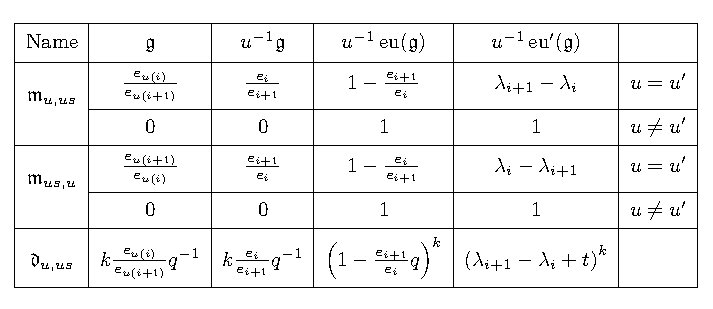
\includegraphics[width=12cm]{figures/table/table_euler_class_q.pdf}
      \caption{}
      \label{table:euler_class_2}        
\end{table}

\begin{theorem}\label{thm:Demazure_operator_2}
When the quiver has no cycle, we have a formula of Demazure operator for the $G_{\dimvec{d}} \times \mathbb{C}^{\times}$-action:
\begin{equation*}\label{eq:Demazure_operator_C*action}
D_i^{u,u'} \star f^{u'}=\begin{cases}
\left[\left( \raisebox{1mm}{$\displaystyle\frac{s_i f}{ 1-\frac{e_{i+1}}{e_{i}}}     + \frac{f}{1-\frac{e_{i}}{e_{i+1}}}$}  \right)\left(\displaystyle 1-\frac{e_{i+1}}{e_{i}} q\right)^{k} \right]^{u} & u=u',\\[8mm]
\left[s_i f  \left(\displaystyle 1-\frac{e_{i+1}}{e_{i}} q\right)^{k} \right]^{u} & u \neq u'.
\end{cases}
\end{equation*}
and similar for the equivariant cohomology:
\begin{equation*}\label{eq:Demazure_operator_cth_C*action}
\partial_i^{u,u'} \star f^{u'}=\begin{cases}
\left[\left( \displaystyle\frac{s_i f}{ \lambda_{i+1}-\lambda_{i}}     + \frac{f}{\lambda_{i}-\lambda_{i+1} }  \right)\left(\lambda_{i+1}-\lambda_{i} +t \right)^{k} \right]^{u} & u=u',\\[8mm]
\left[s_i f  \left(\lambda_{i+1}-\lambda_{i} +t\right)^{k} \right]^{u} & u \neq u'.
\end{cases}
\end{equation*}
\end{theorem}
%%%%%%%%%%%%%%%%%%%%%%%%%%%%%%%%%%%%%%%%%%%%%%%%%%%%%%%%%%%%%%%%%%%%%%%%%%%%%%%%%%%%%%%%%%%%%
\section{From formula to diagram}\label{sec:diagram}
This section is designed for showing examples. Recall Proposition \ref{prop:5-case-0.05} that every $\ftdimvec{d}$ or $u$ corresponds to an ordered set of colored points. It can be imagined that the lines connecting two ordered sets represents one element in $K^{G_{\dimvec{d}}}(\St_{\dimvec{d}})$. Actually, we draw the picture of generators of $K^{G_{\dimvec{d}}}(\St_{\dimvec{d}})$ in Figure \ref{fig:generators}, where
$$e_{i}^{u}=:e_{u^{-1}(i)} \left[ \RRep_{u}(Q) \right]^{G_{\dimvec{d}}} \in K^{G_{\dimvec{d}}} \left( \RRep_{u}(Q) \right) \hookrightarrow K^{G_{\dimvec{d}}} \left( \St^{u,u} \right).$$

\begin{figure}[ht]
  \vspace{0cm}
    \centering  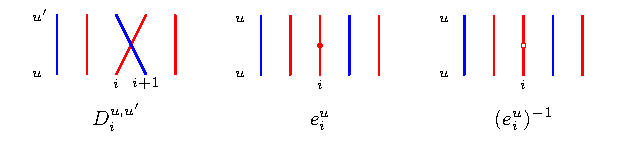
\includegraphics[width=12cm]{figures/strands/generators.pdf}
      \caption{}
      \label{fig:generators}        
\end{figure}

The convolution product can be then viewed as pictures gluing vertically, where the incompatibility of colors gives $0$. For example,

\begin{figure}[ht]
  \vspace{0cm}
    \centering  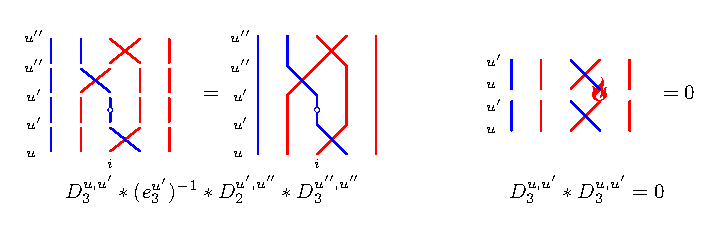
\includegraphics[width=12cm]{figures/strands/glue_vertically.pdf}
      \label{fig:glue_vertically}        
\end{figure}

By Proposition \ref{prop:generators}, every element in $K^{G_{\dimvec{d}}}(\St_{\dimvec{d}})= \oplus_{u,u'} K^{G_{\dimvec{d}}}(\St^{u,u'})$  can be expressed as a $\mathbb{Z}$-linear combination of strands. The expressions are not unique, so we need to find out their relations. Some relations are clear from the picture (but still need to check), for example,

\begin{figure}[ht]
  \vspace{0cm}
    \centering  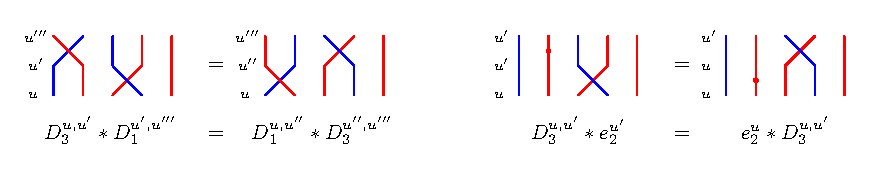
\includegraphics[width=15cm]{figures/strands/clear_relations.pdf}
      \label{fig:clear_relations}        
\end{figure}

We won't draw these ``obvious" relations later. The first nontrivial relation comes from the following lemma.

\begin{lemma}\label{lem:convolution_product_1}
For $f \in \Rpt(T_{\dimvec{d}})$, denote $D_i^{u,u'} =\left[\St_{s_{i}}^{u,u'}\right]^{G_{\dimvec{d}}}$, $f^{u}=f \cdot \left[ \RRep_{\dimvec{d}}(Q) \right]^{G_{\dimvec{d}}} \in K^{G_{\dimvec{d}}} (\St_{\dimvec{d}})$, we have
$$D_i^{u,u'} \fakestar f^{u'}= (s_i f)^{u} \fakestar D_i^{u,u'} +  \delta_{u,u'}\left[\left(s_i f-f\right) \frac{e_{i+1}}{e_i}  \left(\displaystyle 1-\frac{e_{i+1}}{e_{i}}\right)^{k-1} \right]^{u}.$$
Similarly, for the $G_{\dimvec{d}}$-equivariant cohomology, we have
$$\partial_i^{u,u'} \fakestar f^{u'}= (s_i f)^{u} \fakestar \partial_i^{u,u'} +  \delta_{u,u'}\left[\left(s_i f-f\right)   \left(\lambda_{i+1}-\lambda_{i}\right)^{k-1} \right]^{u}.$$
In the formula, $k$ stands for the number of arrows from the vertex associated to $v_{u(i+1)}$ to the vertex associated to $v_{u(i)}$.
\end{lemma}
\begin{proof}
By Proposition \ref{prop:generators}, we only need to show, for any $g \in \Rpt(T_{\dimvec{d}})$,
$$D_i^{u,u'} \fakestar f^{u'} \star g^{u'}= (s_i f)^{u} \fakestar D_i^{u,u'} \star g^{u'} +  \delta_{u,u'}\left[\left(s_i f-f\right) \frac{e_{i+1}}{e_i}  \left(\displaystyle 1-\frac{e_{i+1}}{e_{i}}\right)^{k-1} \right]^{u} \star g^{u'}.$$
Now we apply Theorem \ref{thm:Demazure_operator_1}. The same argument works for equivariant cohomology.
\end{proof}
Lemma \ref{lem:convolution_product_1} explains ``what happens when a point walk through a crossing". The convolution algebra $H_{G_{\dimvec{d}}}^{*}(\St_{\dimvec{d}})$ is called the \textbf{KLR algebra}. The relations of the KLR algebra can be found in \cite[Definition 3.2.2]{seiffarth2017klr}, and we will only show the relations of $K$-theoretic version.
\begin{warning}
In the following examples, $\fakestar$ is often omitted for simplicity.
\end{warning}
\subsection{One point quiver}
We begin with the trivial quiver, which has only one vertex and no arrows. Everything is simplified: 
$$\WWd=\Wd,\quad \MinWd =\{\Id \}, \quad \RRep_{\dimvec{d}}(Q) \cong \mathcal{F}_{\dimvec{d}}, \quad \St_{\dimvec{d}} \cong\mathcal{F}_{\dimvec{d}} \times \mathcal{F}_{\dimvec{d}},$$
$$K^{G_{\dimvec{d}}} (\mathcal{F}_{\dimvec{d}}) \cong \mathbb{Z}\!\left[ e_1^{\pm 1},\ldots,e_{\abdimvec{d}}^{\pm 1} \right], \qquad H_{G_{\dimvec{d}}}^{*}(\mathcal{F}_{\dimvec{d}}) \cong \mathbb{Q}[\lambda_1,\ldots,\lambda_{\abdimvec{d}}].$$
In this case, $K^{G_{\dimvec{d}}} (\mathcal{F}_{\dimvec{d}} \times  \mathcal{F}_{\dimvec{d}})$ is called the \textbf{$\boldsymbol{K}$-theoretic NilHecke algebra}, and $H_{G_{\dimvec{d}}}^{*}(\mathcal{F}_{\dimvec{d}} \times  \mathcal{F}_{\dimvec{d}})$ is called the \textbf{(cohomological) NilHecke algebra}.

The formulas in Theorem \ref{thm:Demazure_operator_1} and Lemma \ref{lem:convolution_product_1} are simplified: (superscripts are omitted, and functions $f$ in four formulas lie in $K^{G_{\dimvec{d}}} (\mathcal{F}_{\dimvec{d}})$, $K^{G_{\dimvec{d}}} (\mathcal{F}_{\dimvec{d}} \times  \mathcal{F}_{\dimvec{d}})$, $H_{G_{\dimvec{d}}}^{*}(\mathcal{F}_{\dimvec{d}})$ and $H_{G_{\dimvec{d}}}^{*}(\mathcal{F}_{\dimvec{d}} \times  \mathcal{F}_{\dimvec{d}})$, respectively)
\begin{equation*}
\begin{aligned}
  D_i \star f =\;& \frac{s_i f}{1- \frac{e_{i+1}}{e_i}} + \frac{f}{1- \frac{e_{i}}{e_{i+1}}}\\ 
  \partial_i \star f =\;& \frac{s_i f}{\lambda_{i+1}-\lambda_{i}}+\frac{ f}{\lambda_{i}-\lambda_{i+1}}=\frac{f -s_i f}{\lambda_{i}-\lambda_{i+1}}\\
  D_i f =\;& (s_i f) D_i + \frac{f- s_i f}{1- \frac{e_{i}}{e_{i+1}}}\\ 
  \partial_i f =\;& (s_i f) \partial_i + \frac{f- s_i f}{\lambda_{i}-\lambda_{i+1}}\\   
\end{aligned}
\end{equation*}

The relations for $D_i$ are shown in Figure \ref{fig:relations_1}.
\begin{figure}[ht]
  \vspace{0cm}
    \centering 
    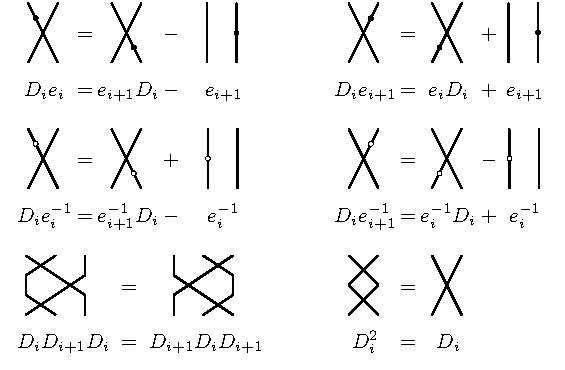
\includegraphics[width=10cm]{figures/strands/relations_1.pdf} 
    \caption{}
      \label{fig:relations_1}        
\end{figure}
\subsection{$A_2$-quiver}
Now let us consider the $A_2$-quiver $\begin{tikzcd}[ampersand replacement=\&]
	\textcolor{red}{\bullet} \& \textcolor{blue}{\bullet} 
	\arrow[from=1-1, to=1-2]
 \end{tikzcd}$. This time we have to color the dots and strands. In this case,
$$K^{G_{\dimvec{d}}} \left(\RRep_{\dimvec{d}}(Q)\right) \cong \bigoplus_{u} \mathbb{Z}\!\left[ e_1^{u,\pm 1},\ldots,e_{\abdimvec{d}}^{u,\pm 1} \right], \qquad H_{G_{\dimvec{d}}}^{*}\!\!\left(\RRep_{\dimvec{d}}(Q)\right) \cong \bigoplus_{u} \mathbb{Q}\left[\lambda_1^{u},\ldots,\lambda_{\abdimvec{d}}^{u}\right].$$
The formulas in Theorem \ref{thm:Demazure_operator_1} and Lemma \ref{lem:convolution_product_1} are simplified: 
\begingroup
\allowdisplaybreaks
\begin{align*}
  D_i^{u,u'} \star f^{u'}=\;&\begin{cases}
  \left[ \raisebox{1mm}{$\displaystyle\frac{s_i f}{ 1-\frac{e_{i+1}}{e_{i}}}     + \frac{f}{1-\frac{e_{i}}{e_{i+1}}}$}   \right]^{u} & \text{\small\raisebox{-0.5mm}{\ding{192}}}\begin{tikzcd}[ampersand replacement=\&]
    	u=u'
     \end{tikzcd},\\[4mm]
  \left[s_i f  \left(\displaystyle 1-\frac{e_{i+1}}{e_{i}}\right) \right]^{u} & \text{\small\raisebox{-0.5mm}{\ding{193}}}\begin{tikzcd}[ampersand replacement=\&]
  	\textcolor{red}{u(i+1)} \& \textcolor{blue}{u(i)} 
  	\arrow[from=1-1, to=1-2]
   \end{tikzcd},\\[3mm]
  \left(s_i f \right)^{u} & \text{\small\raisebox{-0.5mm}{\ding{194}}}\begin{tikzcd}[ampersand replacement=\&]
    	\textcolor{red}{u(i)} \& \textcolor{blue}{u(i+1)} 
    	\arrow[from=1-1, to=1-2]
     \end{tikzcd}.\\
  \end{cases}\\ 
  \partial_i^{u,u'} \star f^{u'}=\;&\begin{cases}
  \left[\displaystyle\frac{f - s_i f}{ \lambda_i-\lambda_{i+1}}  \right]^{u} \hspace{16mm}$\,$& \text{\small\raisebox{-0.5mm}{\ding{192}}}\begin{tikzcd}[ampersand replacement=\&]
      	u=u'
       \end{tikzcd},\\[3mm]
  \left[s_i f  \left(\lambda_{i+1}-\lambda_i\right) \right]^{u} & \text{\small\raisebox{-0.5mm}{\ding{193}}}\begin{tikzcd}[ampersand replacement=\&]
  	\textcolor{red}{u(i+1)} \& \textcolor{blue}{u(i)} 
  	\arrow[from=1-1, to=1-2]
   \end{tikzcd},\\[3mm]
  \left(s_i f \right)^{u} &\text{\small\raisebox{-0.5mm}{\ding{194}}} \begin{tikzcd}[ampersand replacement=\&]
    	\textcolor{red}{u(i)} \& \textcolor{blue}{u(i+1)} 
    	\arrow[from=1-1, to=1-2]
     \end{tikzcd}.\\
  \end{cases}\\ 
  D_i^{u,u'} f^{u'} =\;& (s_i f)^{u} D_i^{u,u'} + \left[\frac{f- s_i f}{1- \frac{e_{i}}{e_{i+1}}}\right]^{u}\\ 
  \partial_i^{u,u'} f^{u'} =\;& (s_i f)^{u} \partial_i^{u,u'} + \left[\frac{f- s_i f}{\lambda_{i}-\lambda_{i+1}}\right]^{u}\\   
\end{align*}
\endgroup

Part of relations for $D_i$ are shown in Figure \ref{fig:relations_2}.
\begin{figure}[ht]
  \vspace{0cm}
    \centering  
    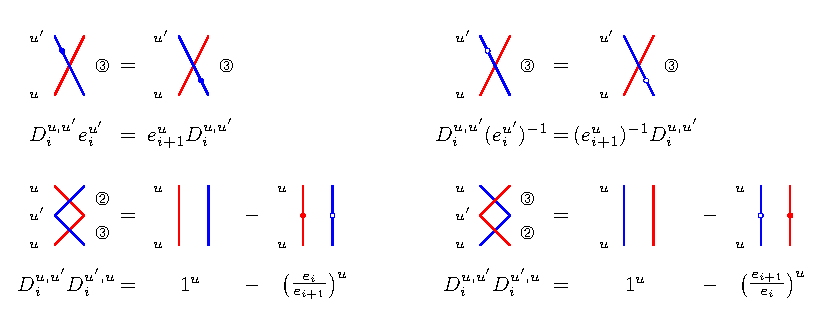
\includegraphics[width=13cm]{figures/strands/relations_2.pdf} 
    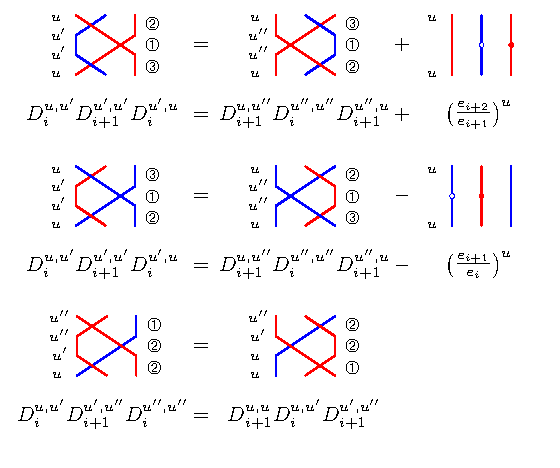
\includegraphics[width=10cm]{figures/strands/relations_3.pdf} 
    \caption{}
      \label{fig:relations_2}        
\end{figure}
\subsection{$1$-loop quiver}
In this subsection we try to give a simplest example for Section \ref{sec:generalization}, which is the $1$-loop quiver. In this case,
$$K^{G_{\dimvec{d}}} \left(\RRep_{\dimvec{d},\str}(Q)\right) \cong  \mathbb{Z}\!\left[ e_1^{\pm 1},\ldots,e_{\abdimvec{d}}^{\pm 1} \right], \qquad H_{G_{\dimvec{d}}}^{*}\!\!\left(\RRep_{\dimvec{d},\str}(Q)\right) \cong  \mathbb{Q}\left[\lambda_1,\ldots,\lambda_{\abdimvec{d}}\right].$$
The formulas in Theorem \ref{thm:Demazure_operator_1} and Lemma \ref{lem:convolution_product_1} are simplified:

\begin{equation*}
\begin{aligned}
  D_i \star f =\;& s_i f + f\cdot \frac{e_{i+1}}{e_{i}}\\ 
  \partial_i \star f =\;& f -s_i f\\
  D_i f =\;& (s_i f) D_i + (s_i f-f) \frac{e_{i+1}}{e_i}\\ 
  \partial_i f =\;& (s_i f) \partial_i + (s_i f-f)\\   
\end{aligned}
\end{equation*}

Now for the $G_{\dimvec{d}} \times \mathbb{C}^{\times}$-action. We have analog of Lemma \ref{lem:convolution_product_1} for $G_{\dimvec{d}} \times \mathbb{C}^{\times}$-action:
\begin{lemma}\label{lem:convolution_product_2}
For $f \in \Rpt(T_{\dimvec{d}} \times \mathbb{C}^{\times})$, denote $D_i^{u,u'} =\left[\St_{s_{i}}^{u,u'}\right]^{G_{\dimvec{d}}\times \mathbb{C}^{\times}}$, $f^{u}=f \cdot \left[ \RRep_{\dimvec{d}}(Q) \right]^{G_{\dimvec{d}}\times \mathbb{C}^{\times}} \in K^{G_{\dimvec{d}}\times \mathbb{C}^{\times}} (\St_{\dimvec{d}})$, we have
$$D_i^{u,u'} \fakestar f^{u'}= (s_i f)^{u} \fakestar D_i^{u,u'} +  \delta_{u,u'}\left[\left(f-s_i f\right) \raisebox{-1mm}{$\displaystyle\frac{\left( 1-\frac{e_{i+1}}{e_{i}} q\right)^{k}}{ 1-\frac{e_{i}}{e_{i+1}}}$}\right]^{u}.$$
Similarly, for the $(G_{\dimvec{d}}\times \mathbb{C}^{\times})$-equivariant cohomology, we have
$$\partial_i^{u,u'} \fakestar f^{u'}= (s_i f)^{u} \fakestar \partial_i^{u,u'} +  \delta_{u,u'}\left[\left(f-s_i f\right) 
\frac{\left(\lambda_{i+1}-\lambda_{i}+t\right)^{k}}{\lambda_{i}-\lambda_{i+1}}   \right]^{u}.$$
In the formula, $k$ stands for the number of arrows from the vertex associated to $v_{u(i+1)}$ to the vertex associated to $v_{u(i)}$.
\end{lemma}
In the $1$-loop quiver case, notice that
$$K^{G_{\dimvec{d}} \times \mathbb{C}^{\times}} \left(\RRep_{\dimvec{d},\str}(Q)\right) \cong  \mathbb{Z}\left[q^{\pm 1}\right]\!\left[ e_1^{\pm 1},\ldots,e_{\abdimvec{d}}^{\pm 1} \right], \quad H_{G_{\dimvec{d}}\times \mathbb{C}^{\times}}^{*}\!\!\left(\RRep_{\dimvec{d},\str}(Q)\right) \cong  \mathbb{Q}[t]\left[\lambda_1,\ldots,\lambda_{\abdimvec{d}}\right].$$

The formulas in Theorem \ref{thm:Demazure_operator_2} and Lemma \ref{lem:convolution_product_2} are simplified:

\begin{equation*}
\begin{aligned}
  D_i \star f=\;&
  \left( \raisebox{1mm}{$\displaystyle\frac{s_i f}{ 1-\frac{e_{i+1}}{e_{i}}}     + \frac{f}{1-\frac{e_{i}}{e_{i+1}}}$}  \right)\left(\displaystyle 1-\frac{e_{i+1}}{e_{i}} q\right)^{k} \\
  \partial_i \star f =\;& (f -s_i f) \frac{\lambda_{i+1}-\lambda_{i}+t}{\lambda_{i}-\lambda_{i+1}}\\
  D_i f =\;& (s_i f) D_i + \left(f-s_i f\right) \displaystyle\frac{ 1-\frac{e_{i+1}}{e_{i}} q}{ 1-\frac{e_{i}}{e_{i+1}}}\\ 
  \partial_i f =\;& (s_i f) \partial_i + (f-s_i f) \frac{\lambda_{i+1}-\lambda_{i}+t}{\lambda_{i}-\lambda_{i+1}}\\   
\end{aligned}
\end{equation*}
Readers are welcomed to write a complete set of relations.
%??? Center of the algebra can be also computed
%%%%%%%%%%%%%%%%%%%%%%%%%%%%%%%%%%%%%%%%%%%%%%%%%%%%%%%%%%%%%%%%%%%%%%%%%%%%%%%%%%%%%%%%%%%%%
\section{Atiyah--Segal completion theorem}\label{sec:AScompletion}

Different cohomology theories are connected in a incredible way. In this section, we describe the Atiyah--Segal completion theorem, which connect $G$-equivariant $K$-theory with $G$-equivariant cohomology. Roughly speaking, they are isomorphic after completion (and base change to $\mathbb{Q}$).

For an algebraic group $G$, we define
$$I:= \ker \left(\Rpt(G) \longrightarrow \Rpt(\Id) \right) \qquad J:= \ker \left(\Spt(G) \longrightarrow \Spt(\Id) \right)$$
as the augmentation ideals in $\Rpt(G)$ and $\Spt(G)$, respectively. We define
$$K^G(X)_I^{\wedge}:= \varprojlim_n K^G(X)/\left(I^n K^G(X) \right) \qquad H_G^{*}(X)_J^{\wedge}:= \varprojlim_n H_G^{*}(X)/\left(J^n H_G^{*}(X) \right)$$
as the $I$-adic (resp. $J$-adic) completion.

\begin{theorem}[Atiyah--Segal completion theorem]\label{thm:Atiyah--Segal_completion_theorem}
For a $G$-variety $X$, the Atiyah--Segal map from the equivariant $K$-theory to the ordinary topological $K$-theory
$$\AS:K^G(X)_I^{\wedge} \longrightarrow K(\EGG G \times^G X ) $$
is an isomorphism, and the (cohomology) Chern class map (defined in \cite[5.8]{chriss1997representation})
$$\chern: K(\EGG G \times^G X ) \longrightarrow H_G^{*}(X)_J^{\wedge}$$
is an isomorphism after base change to $\mathbb{Q}$.
\end{theorem}

Instead of explaining terminologies in Theorem \ref{thm:Atiyah--Segal_completion_theorem}, let us see some examples and get a feeling how that works.

\begin{eg}
For $G=\mathbb{C}^{\times}$,
$$\Rpt(\mathbb{C}^{\times}) \cong \mathbb{Z}\!\left[e^{\pm 1} \right], I=(e-1), \quad \Spt(\mathbb{C}^{\times}) \cong \mathbb{Q}\!\left[\lambda \right], J=(\lambda), $$
we get the following diagram:
% https://q.uiver.app/?q=WzAsMTIsWzEsMCwiS157XFxtYXRoYmJ7Q31ee1xcdGltZXN9fVxcIShcXHB0KV9JXntcXHdlZGdlfSJdLFsyLDAsIksoXFxCR0cgXFxtYXRoYmJ7Q31ee1xcdGltZXN9KSJdLFszLDAsIkhfe1xcbWF0aGJie0N9XntcXHRpbWVzfX1eeyp9XFwhKFxccHQpX0pee1xcd2VkZ2V9Il0sWzAsMCwiS157XFxtYXRoYmJ7Q31ee1xcdGltZXN9fVxcIShcXHB0KSJdLFs0LDAsIkhfe1xcbWF0aGJie0N9XntcXHRpbWVzfX1eeyp9XFwhKFxccHQpIl0sWzAsMSwiXFxtYXRoYmJ7Wn1cXCFcXGxlZnRbZV57XFxwbSAxfSBcXHJpZ2h0XSJdLFsxLDEsIlxcbWF0aGJie1p9XFwhXFxsZWZ0W1xcbGVmdFtlLTFcXHJpZ2h0XSBcXHJpZ2h0XSJdLFsyLDEsIlxcbWF0aGJie1p9XFwhXFxsZWZ0W1xcbGVmdFtlLTFcXHJpZ2h0XSBcXHJpZ2h0XSJdLFszLDEsIlxcbWF0aGJie1F9XFwhXFxsZWZ0W1xcbGVmdFtcXGxhbWJkYVxccmlnaHRdIFxccmlnaHRdIl0sWzQsMSwiXFxtYXRoYmJ7UX1cXCFcXGxlZnRbXFxsYW1iZGEgXFxyaWdodF0iXSxbMiwyLCJlLTEiXSxbMywyLCJlXntcXGxhbWJkYX0tMSJdLFswLDEsIlxcQVMiXSxbMSwyLCJcXGNoZXJuIl0sWzYsN10sWzcsOF0sWzMsMCwiXFxzdWJzZXRlcSIsMSx7InN0eWxlIjp7ImJvZHkiOnsibmFtZSI6Im5vbmUifSwiaGVhZCI6eyJuYW1lIjoibm9uZSJ9fX1dLFs1LDYsIlxcc3Vic2V0ZXEiLDEseyJzdHlsZSI6eyJib2R5Ijp7Im5hbWUiOiJub25lIn0sImhlYWQiOnsibmFtZSI6Im5vbmUifX19XSxbNCwyLCJcXHN1cHNldGVxIiwxLHsic3R5bGUiOnsiYm9keSI6eyJuYW1lIjoibm9uZSJ9LCJoZWFkIjp7Im5hbWUiOiJub25lIn19fV0sWzksOCwiXFxzdXBzZXRlcSIsMSx7InN0eWxlIjp7ImJvZHkiOnsibmFtZSI6Im5vbmUifSwiaGVhZCI6eyJuYW1lIjoibm9uZSJ9fX1dLFsxMCwxMSwiIiwwLHsic3R5bGUiOnsidGFpbCI6eyJuYW1lIjoibWFwcyB0byJ9fX1dXQ==
\[\begin{tikzcd}[column sep={between origins, 30mm}, row sep={between origins, 7mm}]
	{K^{\mathbb{C}^{\times}}\!(\pt)} &[-10mm] {K^{\mathbb{C}^{\times}}\!(\pt)_I^{\wedge}} & {K(\BGG \mathbb{C}^{\times})} & {H_{\mathbb{C}^{\times}}^{*}\!(\pt)_J^{\wedge}} &[-10mm] {H_{\mathbb{C}^{\times}}^{*}\!(\pt)} \\
	{\mathbb{Z}\!\left[e^{\pm 1} \right]} & {\mathbb{Z}\!\left[\left[e-1\right] \right]} & {\mathbb{Z}\!\left[\left[e-1\right] \right]} & {\mathbb{Q}\!\left[\left[\lambda\right] \right]} & {\mathbb{Q}\!\left[\lambda \right]} \\
	&& {e-1} & {e^{\lambda}-1}
	\arrow["\AS", from=1-2, to=1-3]
	\arrow["\chern", from=1-3, to=1-4]
	\arrow[from=2-2, to=2-3]
	\arrow[from=2-3, to=2-4]
	\arrow["\subseteq"{description}, draw=none, from=1-1, to=1-2]
	\arrow["\subseteq"{description}, draw=none, from=2-1, to=2-2]
	\arrow["\supseteq"{description}, draw=none, from=1-5, to=1-4]
	\arrow["\supseteq"{description}, draw=none, from=2-5, to=2-4]
	\arrow[maps to, from=3-3, to=3-4]
\end{tikzcd}\]
This can be generalized to any torus $T$ of rank $n$.
\end{eg}

\begin{eg}\label{eg:AS_initial}
For $G=\GL_n$, $X=\mathcal{F}$,
\begin{equation*}
\begin{aligned}
   \Rpt(\GL_n) \cong\;& \mathbb{Z}\!\left[ e_1^{\pm 1},\ldots,e_n^{\pm 1} \right]^{S_n}, &&I'=\left\{ f \in \Rpt(\GL_n)  \;\middle|\;\rule{0mm}{3.6mm} f(1,\ldots, 1)=0 \right\}\\ 
  \Spt(\GL_n) \cong\;&  \mathbb{Q}\!\left[ \lambda_1,\ldots,\lambda_n \right]^{S_n},&&J'=\left\{ f \in \Spt(\GL_n)  \;\middle|\;\rule{0mm}{3.6mm} f(0,\ldots, 0)=0 \right\}.
\end{aligned}
\end{equation*}
We have the commutative diagram
% https://q.uiver.app/?q=WzAsMTAsWzEsMCwiS157XFxHTF9ufSAoXFxtYXRoY2Fse0Z9KV97SSd9XntcXHdlZGdlfSJdLFsyLDAsIksoXFxFR0cgR0xfbiBcXHRpbWVzXntcXEdMX259XFxtYXRoY2Fse0Z9KSJdLFszLDAsIkhfe0dMX259XnsqfVxcIShcXG1hdGhjYWx7Rn0pX3tKJ31ee1xcd2VkZ2V9Il0sWzAsMCwiS157XFxHTF9ufSAoXFxtYXRoY2Fse0Z9KSJdLFs0LDAsIkhfe0dMX259XnsqfVxcIShcXG1hdGhjYWx7Rn0pIl0sWzAsMSwiS157VH0gKFxccHQpIl0sWzEsMSwiS157VH0gKFxccHQpX3tJfV57XFx3ZWRnZX0iXSxbMiwxLCJLKEJUKSJdLFszLDEsIkhfe1R9XnsqfVxcIShcXHB0KV97Sn1ee1xcd2VkZ2V9Il0sWzQsMSwiSF97VH1eeyp9XFwhKFxccHQpIl0sWzAsMSwiXFxBUyJdLFsxLDIsIlxcY2hlcm4iXSxbNiw3LCJcXEFTIl0sWzcsOCwiXFxjaGVybiJdLFszLDAsIlxcc3Vic2V0ZXEiLDEseyJzdHlsZSI6eyJib2R5Ijp7Im5hbWUiOiJub25lIn0sImhlYWQiOnsibmFtZSI6Im5vbmUifX19XSxbNSw2LCJcXHN1YnNldGVxIiwxLHsic3R5bGUiOnsiYm9keSI6eyJuYW1lIjoibm9uZSJ9LCJoZWFkIjp7Im5hbWUiOiJub25lIn19fV0sWzQsMiwiXFxzdXBzZXRlcSIsMSx7InN0eWxlIjp7ImJvZHkiOnsibmFtZSI6Im5vbmUifSwiaGVhZCI6eyJuYW1lIjoibm9uZSJ9fX1dLFs5LDgsIlxcc3Vwc2V0ZXEiLDEseyJzdHlsZSI6eyJib2R5Ijp7Im5hbWUiOiJub25lIn0sImhlYWQiOnsibmFtZSI6Im5vbmUifX19XSxbNCw5XSxbMiw4XSxbMSw3XSxbMCw2XSxbMyw1XV0=
\[\begin{tikzcd}[
  row sep=small,column sep={between origins, 40mm},
  ar symbol/.style = {draw=none,"\textstyle#1" description,sloped},
  isomorphic/.style = {ar symbol={\cong}},
  ]
	{K^{\GL_n} (\mathcal{F})} &[-19mm] {K^{\GL_n} (\mathcal{F})_{I'}^{\wedge}} & {K\left(\EGG GL_n \times^{\GL_n}\mathcal{F}\right)} & {H_{GL_n}^{*}\!(\mathcal{F})_{J'}^{\wedge}} &[-20mm] {H_{GL_n}^{*}\!(\mathcal{F})} \\
	{K^{T} (\pt)} & {K^{T} (\pt)_{I}^{\wedge}} & {K(BT)} & {H_{T}^{*}\!(\pt)_{J}^{\wedge}} & {H_{T}^{*}\!(\pt)}
	\arrow["\AS", from=1-2, to=1-3]
	\arrow["\chern", from=1-3, to=1-4]
	\arrow["\AS", from=2-2, to=2-3]
	\arrow["\chern", from=2-3, to=2-4]
	\arrow["\subseteq"{description}, draw=none, from=1-1, to=1-2]
	\arrow["\subseteq"{description}, draw=none, from=2-1, to=2-2]
	\arrow["\supseteq"{description}, draw=none, from=1-5, to=1-4]
	\arrow["\supseteq"{description}, draw=none, from=2-5, to=2-4]
	\arrow[from=1-5, to=2-5, isomorphic]
	\arrow[from=1-4, to=2-4, isomorphic]
	\arrow[from=1-3, to=2-3, isomorphic]
	\arrow[from=1-2, to=2-2, isomorphic]
	\arrow[from=1-1, to=2-1, isomorphic]
\end{tikzcd}\]
which reduce to Example \ref{eg:AS_initial}.

Under this isomorphism, the Demazure operator $D_i$ is sent to $\partial_i \fakestar \displaystyle\frac{\lambda_{i}-\lambda_{i+1}}{1-\exp(\lambda_{i}-\lambda_{i+1})}$, i.e., the diagram \eqref{eq:Todd_class} commutes:
% https://q.uiver.app/?q=WzAsNCxbMCwwLCJLXntcXEdMX259IChcXG1hdGhjYWx7Rn0pX3tJJ31ee1xcd2VkZ2V9IFxcb3RpbWVzX3tcXG1hdGhiYntafX1cXG1hdGhiYntRfSJdLFsyLDAsIkhfe0dMX259XnsqfVxcIShcXG1hdGhjYWx7Rn0pX3tKJ31ee1xcd2VkZ2V9Il0sWzAsMSwiS157XFxHTF9ufSAoXFxtYXRoY2Fse0Z9KV97SSd9XntcXHdlZGdlfSBcXG90aW1lc197XFxtYXRoYmJ7Wn19XFxtYXRoYmJ7UX0iXSxbMiwxLCJIX3tHTF9ufV57Kn1cXCEoXFxtYXRoY2Fse0Z9KV97Sid9XntcXHdlZGdlfSJdLFsxLDMsIlxccGFydGlhbF9pIFxcZmFrZXN0YXIgXFxmcmFje1xcbGFtYmRhX3tpfS1cXGxhbWJkYV97aSsxfX17MS1lXntcXGxhbWJkYV97aX0tXFxsYW1iZGFfe2krMX19fSJdLFswLDIsIkRfaSIsMl0sWzAsMSwiXFxjaGVybiBcXGNpcmMgXFxBUyJdLFsyLDMsIlxcY2hlcm4gXFxjaXJjIFxcQVMiXV0=
\begin{equation}\label{eq:Todd_class}
\begin{tikzcd}[column sep=large]
	{K^{\GL_n} (\mathcal{F})_{I'}^{\wedge} \otimes_{\mathbb{Z}}\mathbb{Q}} && {H_{GL_n}^{*}\!(\mathcal{F})_{J'}^{\wedge}} \\
	{K^{\GL_n} (\mathcal{F})_{I'}^{\wedge} \otimes_{\mathbb{Z}}\mathbb{Q}} && {H_{GL_n}^{*}\!(\mathcal{F})_{J'}^{\wedge}}
	\arrow["{\partial_i \fakestar \frac{\lambda_{i}-\lambda_{i+1}}{1-e^{\lambda_{i}-\lambda_{i+1}}}}", from=1-3, to=2-3]
	\arrow["{D_i}"', from=1-1, to=2-1]
	\arrow["{\chern \circ \AS}", from=1-1, to=1-3]
	\arrow["{\chern \circ \AS}", from=2-1, to=2-3]
\end{tikzcd}
\end{equation}
\end{eg}

As a quotient of two (different types of) Euler class, the \textbf{Todd class}
$$\Td_i:=\frac{\lambda_{i}-\lambda_{i+1}}{1-e^{\lambda_{i}-\lambda_{i+1}}}$$
measures the noncommutativity of \eqref{eq:Todd_class} when $\partial_i \fakestar \displaystyle\frac{\lambda_{i}-\lambda_{i+1}}{1-\exp(\lambda_{i}-\lambda_{i+1})}$ is replaced by $\partial_i$.
\include{chapters/chapter7}
\part{Affine pavings of partial flag varieties}\label{part:partial_flag_varieties}

\setlist{itemsep=-0.4em}



%%%%%%%%%%%%%%%%%%%%%%%%%%%%%%%%%%%%%%%%%%%%%%%%%%%%%%%%%%%%%%%%%%%%%%%%%%%%%%%%%%%%%%%%%%%%%
%quiver partial flag varieties



\chapter{Preliminaries for Affine Pavings}\label{chap:flag=gr}

The goal of the two chapters is to find an affine paving of the partial flag variety $\Flag{\ftdimvec{f}}(X)$, which generalizes the variety $\Flag{\ftdimvec{d}}(X)$ defined in \ref{rmk:flag_variety_FlagX}. We have constructed some stratifications of most varieties by orbits in Subsection \ref{subsec:stratification_flag_variety} and \ref{subsec:stratification:_incidence_variety}, and some are even affine pavings. For $\Flag{\ftdimvec{f}}(X)$, we have no natural group actions, so we can not find affine pavings by methods in Subsection \ref{subsec:stratification_flag_variety} and \ref{subsec:stratification:_incidence_variety}. To achieve our goal, we extend methods from \cite{irelli2019cell}
 and \cite{maksimau2019flag} as well as techniques from Auslander--Reiten theory.

In this chapter, we realize the partial flag variety $\Flag{\ftdimvec{f}}(X)$ as a quiver Grassmannian of the extended quiver, prove some $\Ext$-vanishing properties, and also give a short introduction of Auslander--Reiten theory. 

\begin{setting}
Throughout Chapter \ref{chap:flag=gr} and \ref{chap:affine_pavings}, $R$ is a $\mathbb{C}$-algebra with unit, and $\catmod(R)$ denotes the category of $R$-modules of finite dimension. For a representation $X\in \rep(Q)$, we denote by $X_i:=e_iX$ the $\mathbb{C}$-linear space at the vertex $i\in v(Q)$. We denote by $P(i)$, $I(i)$ and $S(i)$ the indecomposable projective, injective, simple modules corresponding to the vertex $i$, respectively.
\end{setting}

\section{Extended quiver}
In this section, we introduce the notion of extended quiver which allows to view partial flag varieties as quiver Grassmannians. Intuitively, a flag of quiver representations can be encoded as a subspace of a representation of the extended quiver.

\begin{defn}[Extended quiver]
For a quiver $Q$ and an integer $d \geqslant 1$, the extended quiver\index{extended quiver} $Q_{d}$ is defined as follows:
\begin{itemize}
	\item The vertex set of $Q_d$ is defined as the Cartesian product of the vertex set of $Q$ and $\{1,\ldots,d\}$, i.e.,
	$$v(Q_d)=v(Q) \times \{1,\ldots,d\}.$$
	\item  There are two types of arrows: for each $(i,r) \in v(Q) \times \{1,\ldots,d-1\}$, there is one arrow from $(i,r)$ to $(i,r+1)$; for each arrow $i \longrightarrow j$ in $Q$ and $r \in \{1,\ldots,d\}$, there is one arrow from $(i,r)$ to $(j,r)$.
\end{itemize}
\end{defn}

The extended quiver $Q_d$ is exactly the same quiver as $\hat{\Gamma}_d$ in \cite[Definition 2.2]{maksimau2019flag}. The next definition is a small variation:

\begin{defn}[Strict extended quiver]
For a quiver $Q$ and an integer $d \geqslant 2$, the strict extended quiver $Q_{d,\str}$ is defined as follows:
\begin{itemize}
	\item The vertex set of $Q_d$ is defined as the Cartesian product of the vertex set of $Q$ and $\{1,\ldots,d\}$, i.e.,
	$$v(Q_{d,\str})=v(Q) \times \{1,\ldots,d\}.$$
	\item  We have two types of arrows: for each $(i,r) \in v(Q) \times \{1,\ldots,d-1\}$, there is one arrow from $(i,r)$ to $(i,r+1)$; for each arrow $i \longrightarrow j$ in quiver $Q$ and $r \in \{2,\ldots,d\}$, there is one arrow from $(i,r)$ to $(j,r-1)$.
\end{itemize}
\end{defn}


\begin{eg}\label{eg:ext_quiver}
The (strict) extended quiver for a Dynkin quiver $Q$ of type $A_4$ looks as follows.
% https://q.uiver.app/?q=WzAsMzEsWzAsMiwiXFxidWxsZXQiXSxbMiwyLCJcXGJ1bGxldCJdLFs0LDIsIlxcYnVsbGV0Il0sWzYsMiwiXFxidWxsZXQiXSxbNywyLCJcXGJ1bGxldCJdLFs5LDIsIlxcYnVsbGV0Il0sWzExLDIsIlxcYnVsbGV0Il0sWzEzLDIsIlxcYnVsbGV0Il0sWzcsMSwiXFxidWxsZXQiXSxbOSwxLCJcXGJ1bGxldCJdLFsxMSwxLCJcXGJ1bGxldCJdLFsxMywxLCJcXGJ1bGxldCJdLFs3LDAsIlxcYnVsbGV0Il0sWzksMCwiXFxidWxsZXQiXSxbMTEsMCwiXFxidWxsZXQiXSxbMTMsMCwiXFxidWxsZXQiXSxbMTQsMiwiXFxidWxsZXQiXSxbMTYsMiwiXFxidWxsZXQiXSxbMTQsMSwiXFxidWxsZXQiXSxbMTQsMCwiXFxidWxsZXQiXSxbMTYsMSwiXFxidWxsZXQiXSxbMTgsMSwiXFxidWxsZXQiXSxbMTgsMCwiXFxidWxsZXQiXSxbMjAsMSwiXFxidWxsZXQiXSxbMjAsMiwiXFxidWxsZXQiXSxbMjAsMCwiXFxidWxsZXQiXSxbMTgsMiwiXFxidWxsZXQiXSxbMTYsMCwiXFxidWxsZXQiXSxbMywzLCJcXGhzcGFjZXstMWNtfVFcXGhzcGFjZXstMWNtfSJdLFsxMCwzLCJcXGhzcGFjZXstMWNtfVFfM1xcaHNwYWNley0xY219Il0sWzE3LDMsIlxcaHNwYWNley0xY219UV97MyxzdHJ9XFxoc3BhY2V7LTFjbX0iXSxbMCwxXSxbMiwxXSxbMiwzXSxbNCw1XSxbNiw1XSxbNiw3XSxbOCw5XSxbMTAsOV0sWzEwLDExXSxbMTIsMTNdLFsxNCwxM10sWzE0LDE1XSxbOCwxMl0sWzQsOF0sWzUsOV0sWzksMTNdLFsxMCwxNF0sWzYsMTBdLFs3LDExXSxbMTEsMTVdLFsxOCwxN10sWzE5LDIwXSxbMjEsMTddLFsyMiwyMF0sWzIyLDIzXSxbMjEsMjRdLFsyMywyNV0sWzI0LDIzXSxbMjYsMjFdLFsyMSwyMl0sWzE3LDIwXSxbMjAsMjddLFsxOCwxOV0sWzE2LDE4XV0=
\[\begin{tikzcd}[column sep=3mm, row sep=5mm]
	&&&&&&&[5mm] \bullet && \bullet && \bullet && \bullet &[5mm] \bullet && \bullet && \bullet && \bullet \\
	&&&&&&& \bullet && \bullet && \bullet && \bullet & \bullet && \bullet && \bullet && \bullet \\
	\bullet && \bullet && \bullet && \bullet & \bullet && \bullet && \bullet && \bullet & \bullet && \bullet && \bullet && \bullet \\[-5mm]
	&&& {\hspace{-1cm}Q\hspace{-1cm}} &&&&&&& {\hspace{-1cm}Q_3\hspace{-1cm}} &&&&&&& {\hspace{-1cm}Q_{3,\str}\hspace{-1cm}}
	\arrow[from=3-1, to=3-3]
	\arrow[from=3-5, to=3-3]
	\arrow[from=3-5, to=3-7]
	\arrow[from=3-8, to=3-10]
	\arrow[from=3-12, to=3-10]
	\arrow[from=3-12, to=3-14]
	\arrow[from=2-8, to=2-10]
	\arrow[from=2-12, to=2-10]
	\arrow[from=2-12, to=2-14]
	\arrow[from=1-8, to=1-10]
	\arrow[from=1-12, to=1-10]
	\arrow[from=1-12, to=1-14]
	\arrow[from=2-8, to=1-8]
	\arrow[from=3-8, to=2-8]
	\arrow[from=3-10, to=2-10]
	\arrow[from=2-10, to=1-10]
	\arrow[from=2-12, to=1-12]
	\arrow[from=3-12, to=2-12]
	\arrow[from=3-14, to=2-14]
	\arrow[from=2-14, to=1-14]
	\arrow[from=2-15, to=3-17]
	\arrow[from=1-15, to=2-17]
	\arrow[from=2-19, to=3-17]
	\arrow[from=1-19, to=2-17]
	\arrow[from=1-19, to=2-21]
	\arrow[from=2-19, to=3-21]
	\arrow[from=2-21, to=1-21]
	\arrow[from=3-21, to=2-21]
	\arrow[from=3-19, to=2-19]
	\arrow[from=2-19, to=1-19]
	\arrow[from=3-17, to=2-17]
	\arrow[from=2-17, to=1-17]
	\arrow[from=2-15, to=1-15]
	\arrow[from=3-15, to=2-15]
\end{tikzcd}\]
\end{eg}

Next, we define the quiver algebras for later use.
\begin{defn}[Algebra of an extended quiver]\label{def:bqa}
For an extended quiver $Q_d$, let $\mathbb{C}Q_d$ be the corresponding path algebra, and $I$ be the ideal of $\mathbb{C}Q_d$ identifying all the paths with the same sources and targets. The algebra of the extended quiver $Q_d$ is defined as
$$R_d:= \mathbb{C}Q_d/I.$$
Similarly, we define the algebra $R_{d,\str}:= \mathbb{C}Q_{d,\str}/I$ for the strict extended quiver.
\end{defn}
By abuse of notation, we often abbreviate $R_d$ and $R_{d,\str}$ by $R$. 
\section{Canonical functor $\Phi$}
We follow \cite[2.3]{maksimau2019flag} in this section with a few variations. 
\begin{defn}[Partial flag variety]\label{def:pf}\index{flag variety!partial flag variety}
For a quiver representation $X \in \rep(Q)$ and an integer $d \geqslant 1$, we define
$$\Flagd(X):=\left\{ 0 \subseteq M_1 \subseteq \cdots M_d \subseteq X \right\}$$
as the collection of all partial flags of length $d$, and call it the partial flag variety associated to $X$. 
\end{defn}
\begin{defn}[Strict partial flag variety]\label{def:spf}
For a quiver representation $X \in \rep(Q)$ and an integer $d \geqslant 2$, we define
$$\Flagdstr(X):=\left\{ 0 \subseteq M_1 \subseteq \cdots M_d \subseteq X\mid x.M_{k+1} \subseteq M_k \right\}$$
as the collection of all strict partial flags of length $d$, and call it the strict partial flag variety associated to $X$. 
\end{defn}
\begin{defn}[Grassmannian]
Let $R$ be the bounded quiver algebra defined in Definition \ref{def:pf} or \ref{def:spf}. For a module $T \in \catmod(R)$, the Grassmannian\index{Grassmannian} $\Gralg{R}(T)$ is defined as the set of all submodules of $T$, i.e.,
$$\Gralg{R}(T):=\{T' \subseteq T \text{ as the submodule}  \}.$$
\end{defn}
\begin{defn}[Canonical functor $\Phi$]
The canonical functor\index{canonical functor} $\Phi:\rep(Q) \longrightarrow \catmod(R) $ is defined as follows:
\begin{itemize}
\item $\left(\Phi(X)\right)_{(i,r)}:=X_i$;
\item $\left(\Phi(X)\right)_{(i,r) \rightarrow (i,r+1)}:=\Id_{X_i}$;
\item Either $\left(\Phi(X)\right)_{(i,r) \rightarrow (j,r)}:=X_{i \rightarrow j}$ for $R=R_d$, \\or $\left(\Phi(X)\right)_{(i,r) \rightarrow (j,r-1)}:=X_{i \rightarrow j}$ for $R=R_{d,\str}$.
\end{itemize}
\end{defn}
The functor $\Phi$ helps to realize a partial flag as a quiver subrepresentation. 
\begin{proposition}\label{prop:flag=gr}
For a representation $X\in \rep(Q)$, the canonical functor $\Phi$ induces isomorphisms
$$\Flagd(X)\cong \Gralg{R_d}(\Phi(X)) \qquad \Flagdstr(X)\cong \Gralg{R_{d,\str}}(\Phi(X)).$$
\end{proposition}
\begin{proof}
The isomorphism maps a flag $M:M_1 \subseteq \cdots \subseteq M_d$ to a representation $\Phi'(M)$ with $\Phi'(M)_{(i,r)}=M_{i,r}$ and obvious morphisms for arrows. The non-strict case is mentioned in \cite[page 4]{maksimau2019flag} and the strict case works similarly.
\end{proof}
%https://tex.stackexchange.com/questions/495252/i-want-to-get-a-big-subset
\begin{eg}\label{eg:bigpic}
Consider the quiver $Q\colon x \longrightarrow y \longleftarrow z \longrightarrow w$, and let $X\colon X_x \longrightarrow X_y \longleftarrow X_z \longrightarrow X_w$ be a representation. The varieties $\Flag{3}(X),\Flagstr{3}(X)$ then arise as quiver Grassmannian as shown in Figure \ref{fig:flagasgr}.
	\begin{figure}[ht]
	\centering
		\vspace{0cm}
		\centering
		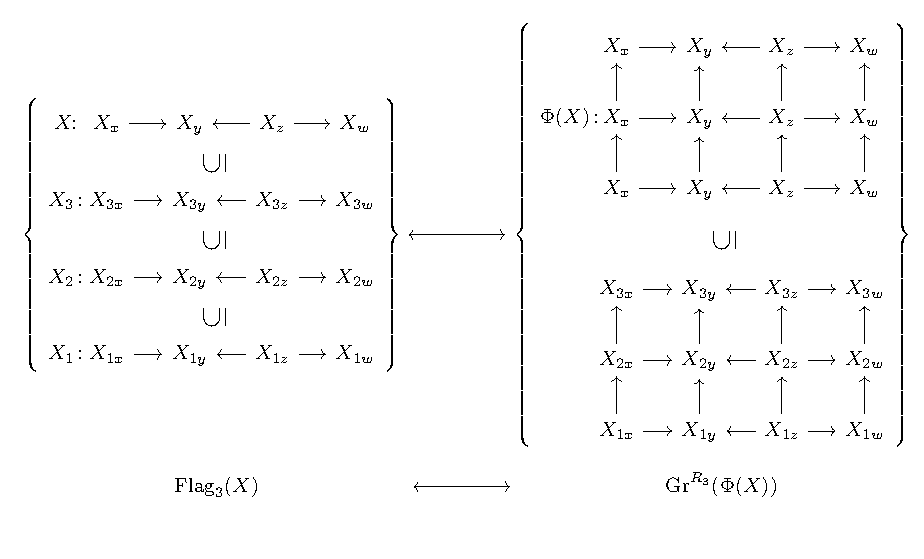
\includegraphics[width=0.81\linewidth]{figures/affine_paving/bigpic.pdf}
		\vspace{-0.5cm}
		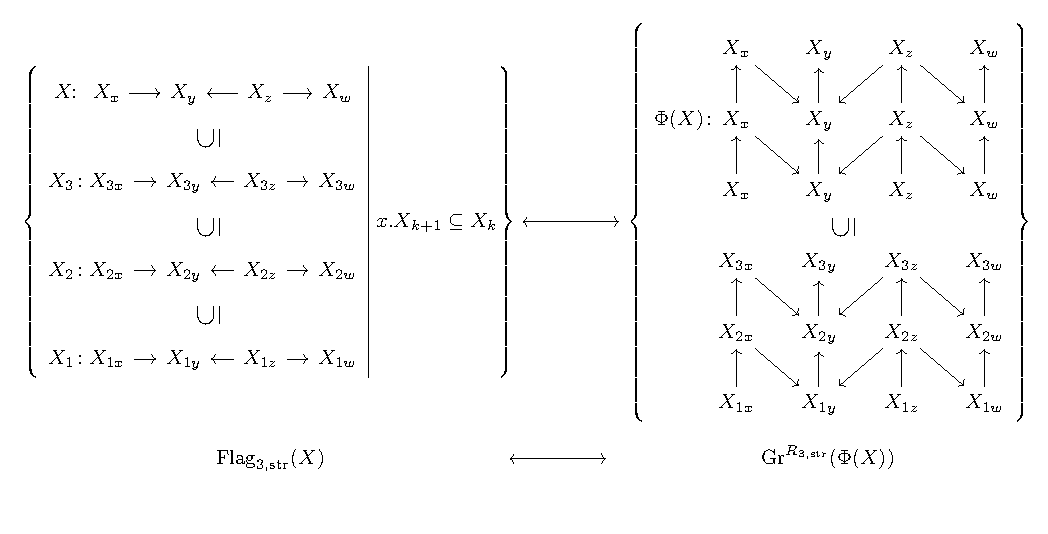
\includegraphics[width=0.9\linewidth]{figures/affine_paving/bigpic2.pdf}
		\vspace{-0.35cm}
%		\captionsetup{labelformat=empty}
		\caption[Realize flag as quiver Grassmannian]{}
		\vspace{0.3cm}
		\label{fig:flagasgr}
	\end{figure}
\end{eg}
In many cases, the proof of the strict case and the non-strict case is the same, so we often treat them in the same way. For example, we may abbreviate the formula in Proposition \ref{prop:flag=gr} as 
$$\Flag{}(X)\cong \Gr(\Phi(X)).$$
\section{Dimension vector}In this section we define some varieties indexed by dimension vectors. Recall Definition \ref{def:Q-vs} and \ref{def:ftdv}. Notice that every module $T \in \catmod(\mathbb{C}Q/I)$ can be viewed as a representation of $Q$, so we automatically have a notion of dimension vector for $T$.

We can write the (strict) partial flag variety and Grassmannian as disjoint union of several pieces. Since $v(Q_{d,(\str)})=v(Q) \times \{1,\ldots,d\}$, any dimension vector $\ftdimvec{f}$ of $R$ can be viewed as $d$ dimension vectors $(\ftdimvec{f}_1,\ldots,\ftdimvec{f}_d)$. Define
\begin{equation*}
\begin{aligned}
  \Flag{\ftdimvec{f}}(X):=\;&\left\{ 0 \subseteq M_1 \subseteq \cdots M_d \subseteq X \;\middle|\; \dimv M_k=\ftdimvec{f}_k \right\} && \subseteq  \Flagd(X), \\ 
  \Flag{\ftdimvec{f},\str}(X):=\;&\left\{ 0 \subseteq M_1 \subseteq \cdots M_d \subseteq X \;\middle|\; x.M_{k+1} \subseteq M_k,\, \dimv M_k=\ftdimvec{f}_k \right\} && \subseteq  \Flagdstr(X), \\ 
  \Gralg{R}_{\ftdimvec{f}}(T):=\;&\{T' \subseteq T \text{ with } \dimv T'=\ftdimvec{f}\} && \subseteq  \Gralg{R}(T). 
\end{aligned}
\end{equation*}
Then from the Proposition \ref{prop:flag=gr} we get 
$$\Flag{\ftdimvec{f}}(X) \cong \Gralg{R_d}_{\ftdimvec{f}}(\Phi(X)) \qquad \Flag{\ftdimvec{f},\str}(X) \cong \Gralg{R_{d,\str}}_{\ftdimvec{f}}(\Phi(X)).$$


Finally, we need to define the Euler form of two dimension vectors. For this we need to define the set of virtual arrows of the quivers $Q_d$ and $Q_{d,\str}$. Following Example \ref{example:virtualarrow}, the virtual arrows of the quivers $Q_3$ and $Q_{3,\str}$ are depicted in red.
\begin{defn}[Virtual arrows of the quiver $Q_d$]
For $d \geqslant 1$, the virtual arrows of the quiver $Q_d$ is defined as a triple $\big(va(Q_d),s,t\big)$, where
$$va(Q_d):=a(Q) \times \{1,\ldots, d-1 \}$$
is a finite set, and $s,t: va(Q_d) \longrightarrow v(Q_d)$ are maps defined by
$$s\big((i\rightarrow j,r)\big)=(i,r) \qquad t \big((i\rightarrow j,r)\big)=(j,r+1).$$
\end{defn}
\begin{defn}[Virtual arrows of the quiver $Q_{d,\str}$]
For $d \geqslant 2$, the virtual arrows\index{virtual arrow} of the quiver $Q_{d,\str}$ is defined as a triple $\big(va(Q_{d,\str}),s,t\big)$, where
$$va(Q_{d,\str}):=a(Q) \times \{2,\ldots, d-1 \}$$
is a finite set, and $s,t: va(Q_{d,\str}) \longrightarrow v(Q_{d,\str})$ are maps defined by
$$s\big((i\rightarrow j,r)\big)=(i,r) \qquad t \big((i\rightarrow j,r)\big)=(j,r).$$
\end{defn}
\begin{eg}\label{example:virtualarrow}
$\qquad$
	\begin{figure}[!ht]
		\vspace{0cm}
		\centering
% https://q.uiver.app/?q=WzAsMzEsWzAsMiwiXFxidWxsZXQiXSxbMiwyLCJcXGJ1bGxldCJdLFs0LDIsIlxcYnVsbGV0Il0sWzYsMiwiXFxidWxsZXQiXSxbNywyLCJcXGJ1bGxldCJdLFs5LDIsIlxcYnVsbGV0Il0sWzExLDIsIlxcYnVsbGV0Il0sWzEzLDIsIlxcYnVsbGV0Il0sWzcsMSwiXFxidWxsZXQiXSxbOSwxLCJcXGJ1bGxldCJdLFsxMSwxLCJcXGJ1bGxldCJdLFsxMywxLCJcXGJ1bGxldCJdLFs3LDAsIlxcYnVsbGV0Il0sWzksMCwiXFxidWxsZXQiXSxbMTEsMCwiXFxidWxsZXQiXSxbMTMsMCwiXFxidWxsZXQiXSxbMTQsMiwiXFxidWxsZXQiXSxbMTYsMiwiXFxidWxsZXQiXSxbMTQsMSwiXFxidWxsZXQiXSxbMTQsMCwiXFxidWxsZXQiXSxbMTYsMSwiXFxidWxsZXQiXSxbMTgsMSwiXFxidWxsZXQiXSxbMTgsMCwiXFxidWxsZXQiXSxbMjAsMSwiXFxidWxsZXQiXSxbMjAsMiwiXFxidWxsZXQiXSxbMjAsMCwiXFxidWxsZXQiXSxbMTgsMiwiXFxidWxsZXQiXSxbMTYsMCwiXFxidWxsZXQiXSxbMywzLCJcXGhzcGFjZXstMWNtfVFcXGhzcGFjZXstMWNtfSJdLFsxMCwzLCJcXGhzcGFjZXstMWNtfVFfM1xcaHNwYWNley0xY219Il0sWzE3LDMsIlxcaHNwYWNley0xY219UV97MyxzdHJ9XFxoc3BhY2V7LTFjbX0iXSxbMCwxXSxbMiwxXSxbMiwzXSxbNCw1XSxbNiw1XSxbNiw3XSxbOCw5XSxbMTAsOV0sWzEwLDExXSxbMTIsMTNdLFsxNCwxM10sWzE0LDE1XSxbOCwxMl0sWzQsOF0sWzUsOV0sWzksMTNdLFsxMCwxNF0sWzYsMTBdLFs3LDExXSxbMTEsMTVdLFsxOCwxN10sWzE5LDIwXSxbMjEsMTddLFsyMiwyMF0sWzIyLDIzXSxbMjEsMjRdLFsyMywyNV0sWzI0LDIzXSxbMjYsMjFdLFsyMSwyMl0sWzE3LDIwXSxbMjAsMjddLFsxOCwxOV0sWzE2LDE4XSxbOCwxMywiIiwxLHsiY29sb3VyIjpbMCwxMDAsNjBdfV0sWzQsOSwiIiwxLHsiY29sb3VyIjpbMCwxMDAsNjBdfV0sWzEwLDEzLCIiLDEseyJjb2xvdXIiOlswLDEwMCw2MF19XSxbNiw5LCIiLDEseyJjb2xvdXIiOlswLDEwMCw2MF19XSxbNiwxMSwiIiwxLHsiY29sb3VyIjpbMCwxMDAsNjBdfV0sWzEwLDE1LCIiLDEseyJjb2xvdXIiOlswLDEwMCw2MF19XSxbMTgsMjAsIiIsMSx7ImNvbG91ciI6WzAsMTAwLDYwXX1dLFsyMSwyMCwiIiwxLHsiY29sb3VyIjpbMCwxMDAsNjBdfV0sWzIxLDIzLCIiLDEseyJjb2xvdXIiOlswLDEwMCw2MF19XV0=
\[\begin{tikzcd}[column sep=3mm, row sep=5mm]
	&&&&&&&[5mm] \bullet && \bullet && \bullet && \bullet &[5mm] \bullet && \bullet && \bullet && \bullet \\
	&&&&&&& \bullet && \bullet && \bullet && \bullet & \bullet && \bullet && \bullet && \bullet \\
	\bullet && \bullet && \bullet && \bullet & \bullet && \bullet && \bullet && \bullet & \bullet && \bullet && \bullet && \bullet \\[-5mm]
	&&& {\hspace{-1cm}Q\hspace{-1cm}} &&&&&&& {\hspace{-1cm}Q_3\hspace{-1cm}} &&&&&&& {\hspace{-1cm}Q_{3,\str}\hspace{-1cm}}
	\arrow[from=3-1, to=3-3]
	\arrow[from=3-5, to=3-3]
	\arrow[from=3-5, to=3-7]
	\arrow[from=3-8, to=3-10]
	\arrow[from=3-12, to=3-10]
	\arrow[from=3-12, to=3-14]
	\arrow[from=2-8, to=2-10]
	\arrow[from=2-12, to=2-10]
	\arrow[from=2-12, to=2-14]
	\arrow[from=1-8, to=1-10]
	\arrow[from=1-12, to=1-10]
	\arrow[from=1-12, to=1-14]
	\arrow[from=2-8, to=1-8]
	\arrow[from=3-8, to=2-8]
	\arrow[from=3-10, to=2-10]
	\arrow[from=2-10, to=1-10]
	\arrow[from=2-12, to=1-12]
	\arrow[from=3-12, to=2-12]
	\arrow[from=3-14, to=2-14]
	\arrow[from=2-14, to=1-14]
	\arrow[from=2-15, to=3-17]
	\arrow[from=1-15, to=2-17]
	\arrow[from=2-19, to=3-17]
	\arrow[from=1-19, to=2-17]
	\arrow[from=1-19, to=2-21]
	\arrow[from=2-19, to=3-21]
	\arrow[from=2-21, to=1-21]
	\arrow[from=3-21, to=2-21]
	\arrow[from=3-19, to=2-19]
	\arrow[from=2-19, to=1-19]
	\arrow[from=3-17, to=2-17]
	\arrow[from=2-17, to=1-17]
	\arrow[from=2-15, to=1-15]
	\arrow[from=3-15, to=2-15]
	\arrow[dashed,color={rgb,255:red,255;green,51;blue,51}, from=2-8, to=1-10]
	\arrow[dashed,color={rgb,255:red,255;green,51;blue,51}, from=3-8, to=2-10]
	\arrow[dashed,color={rgb,255:red,255;green,51;blue,51}, from=2-12, to=1-10]
	\arrow[dashed,color={rgb,255:red,255;green,51;blue,51}, from=3-12, to=2-10]
	\arrow[dashed,color={rgb,255:red,255;green,51;blue,51}, from=3-12, to=2-14]
	\arrow[dashed,color={rgb,255:red,255;green,51;blue,51}, from=2-12, to=1-14]
	\arrow[dashed,color={rgb,255:red,255;green,51;blue,51}, from=2-15, to=2-17]
	\arrow[dashed,color={rgb,255:red,255;green,51;blue,51}, from=2-19, to=2-17]
	\arrow[dashed,color={rgb,255:red,255;green,51;blue,51}, from=2-19, to=2-21]
\end{tikzcd}\]
\vspace{-5mm}
		\label{fig:virtualarrow}
		\vspace{2mm}
	\end{figure}
\end{eg}
\begin{defn}[Euler form of $R$]
Let $R$ be a bounded quiver algebra defined in Definition \ref{def:bqa}. We denote
\begin{equation*}
\begin{aligned}
	v(R):&= \{\text{vertices in $Q_d$ or $Q_{d,\str}$}\}, \\
	a(R):&= \{\text{arrows in $Q_d$ or $Q_{d,\str}$}\}, \\
	va(R):&= \{\text{virtual arrows in $Q_d$ or $Q_{d,\str}$}\}. \\
\end{aligned}
\end{equation*}

For two dimension vectors $\ftdimvec{f},\ftdimvec{g}$ of $R$, the Euler form\index{Euler form} $\left< \ftdimvec{f},\ftdimvec{g}\right>_R$ is defined by
	$$\left< \ftdimvec{f},\ftdimvec{g}\right>_R:= \sum_{i \in v(R)} f_ig_i - \sum_{b \in a(R)} f_{s(b)}g_{t(b)}+ \sum_{c \in va(R)} f_{s(c)}g_{t(c)}.$$
\end{defn}
\section{Ext-vanishing properties}
We will show that some higher rank extension group are zero, which will be a key ingredient in the proofs of Section \ref{sec:mainthm}.

For a bounded quiver algebra $R$ defined in Definition \ref{def:bqa}, we have a standard resolution for every $R$-module $T$: 
% https://q.uiver.app/?q=WzAsMTIsWzAsMCwiMCJdLFsxLDAsIlxcYmlnb3BsdXNfe1xcc3Vic3RhY2t7YyBcXGluIHZhKFEpXFxcXGM9Yl8xY18xPWJfMmNfMn19IFJlX3t0KGMpfSBcXG90aW1lc19LIGVfe3MoYyl9VCJdLFsyLDAsIlxcYmlnb3BsdXNfe2IgXFxpbiBhKFEpfSBSZV97dChiKX0gXFxvdGltZXNfSyBlX3tzKGIpfVQiXSxbMywwLCJcXGJpZ29wbHVzX3tpIFxcaW4gdihRKX0gUmVfe2l9IFxcb3RpbWVzX0sgZV97aX1UIl0sWzQsMCwiVCJdLFs1LDAsIjAiXSxbMSwxLCJyIFxcb3RpbWVzIHgiXSxbMiwxLCJcXHN1YnN0YWNre1xccGhhbnRvbXsrfXJjXzEgXFxvdGltZXMgeCArciBcXG90aW1lcyBiXzF4XFxcXC1yY18yIFxcb3RpbWVzIHggLXIgXFxvdGltZXMgYl8yeH0iXSxbMywxLCJyIFxcb3RpbWVzIHgiXSxbNCwxLCJyeCJdLFsyLDIsInIgXFxvdGltZXMgeCJdLFszLDIsInJiIFxcb3RpbWVzIHgtciBcXG90aW1lcyBieCJdLFswLDFdLFsxLDJdLFsyLDNdLFszLDRdLFs0LDVdLFs2LDcsIiIsMCx7InN0eWxlIjp7InRhaWwiOnsibmFtZSI6Im1hcHMgdG8ifX19XSxbOCw5LCIiLDAseyJzdHlsZSI6eyJ0YWlsIjp7Im5hbWUiOiJtYXBzIHRvIn19fV0sWzEwLDExLCIiLDAseyJzdHlsZSI6eyJ0YWlsIjp7Im5hbWUiOiJtYXBzIHRvIn19fV1d
\[
\begin{tikzcd}[row sep=0mm,column sep=3mm]
	0 & {\displaystyle\bigoplus_{c \in va(Q)} \hspace{-3mm}Re_{t(c)} \otimes_\mathbb{C} e_{s(c)}T} & {\displaystyle\bigoplus_{b \in a(Q)}\hspace{-2mm} Re_{t(b)} \otimes_\mathbb{C} e_{s(b)}T} & {\displaystyle\bigoplus_{i \in v(Q)}\hspace{-2mm} Re_{i} \otimes_\mathbb{C} e_{i}T} & T & 0 \\
	& {\hspace{10mm} r \otimes x} & {\substack{\phantom{+}rc_1 \otimes x +r \otimes b_1x\\-rc_2 \otimes x -r \otimes b_2x}\hspace{-5mm}} & {\hspace{6mm}r \otimes x} & rx \\
	&& {\hspace{6mm}r \otimes x} & {rb \otimes x-r \otimes bx\hspace{-3mm}}
	\arrow[from=1-1, to=1-2]
	\arrow[from=1-2, to=1-3]
	\arrow[from=1-3, to=1-4]
	\arrow[from=1-4, to=1-5]
	\arrow[from=1-5, to=1-6]
	\arrow[maps to, from=2-2, to=2-3]
	\arrow[maps to, from=2-4, to=2-5]
	\arrow[maps to, from=3-3, to=3-4]
\end{tikzcd}
\]
There are exactly two paths of length two from $s(c)$ to $t(c)$ for any virtual arrow $c$, which we denoted by $b_1c_1$ and $b_2c_2$ in the above. By definition, these paths are identified in $R$.

\begin{lemma}\label{lm:Extvan}
Let $M,N \in \rep(Q)$.\\[-8mm]
\begingroup
\upshape
\begin{enumerate}[(1)]
	\item $\gldim R \leqslant 2$;\label{lm:gldim}
	\item The functor $\Phi:\rep(Q) \longrightarrow \catmod(R)$ is exact and fully faithful;\label{lm:functorisexact}
	\item $\Phi$ maps projective module to projective module, and maps injective module to injective module;\label{lm:toproj}
	\item $\Ext^i_{\mathbb{C}Q}(M,N) \cong \Ext^i_{R}(\Phi(M),\Phi(N))$;\label{lm:isoofext}
	\item $\projdim \Phi(M) \leqslant 1. \injdim \Phi(M) \leqslant 1$;\label{lm:projdim}
\end{enumerate}
\endgroup
\end{lemma}
\begin{proof}$\,$

For \ref{lm:gldim}, this follows from the standard resolution.

For \ref{lm:functorisexact}, it follows by direct inspection, see \cite[Lemma 2.3]{maksimau2019flag}.
%if we have the short exact sequence in $\rep(Q)$:
%$$0\longrightarrow X \longrightarrow Y \longrightarrow S \longrightarrow 0$$
%then for each vector $i\in v(Q)$, we have the short exact sequence 
%$$0\longrightarrow X_i \longrightarrow Y_i \longrightarrow S_i \longrightarrow 0,$$
%which is equivalent to the short exact sequence 
%$$0\longrightarrow \Phi(X)_{(i,r)} \longrightarrow \Phi(Y)_{(i,r)} \longrightarrow \Phi(S)_{(i,r)} \longrightarrow 0,$$
%for every vector $(i,r)$ in the extended quiver, so the complex
%$$0\longrightarrow \Phi(X) \longrightarrow \Phi(Y) \longrightarrow \Phi(S) \longrightarrow 0$$
%is exact.

For \ref{lm:toproj}, we reduce to the case of indecomposable projective modules, and observe that $$\Phi(P(i))=P\big((i,1)\big),\qquad\Phi(I(i))=I\big((i,d)\big).$$

For \ref{lm:isoofext}, it comes from the fact that $\Phi$ is fully faithful and maps projective module to projective module.
%the isomorphism 
%$$\Ext^i_{\mathbb{C}Q}(M,N) \cong \Ext^i_{R}(\Phi(M),\Phi(N))$$
%follows by the projective resolution of $M$.
%the surjection of map
%$$\Hom_{\mathbb{C}Q}(M,N) \longrightarrow \Hom_{R}(\Phi(M),\Phi(N))$$
%follows by the commutative diagram:
%
%\begin{center}
%% https://tikzcd.yichuanshen.de/#N4Igdg9gJgpgziAXAbVABwnAlgFyxMJZABgBpiBdUkANwEMAbAVxiRAFkB9LEAX1PSZc+QijIBGKrUYs2XHv0HY8BIuPJT6zVohAA5bnwEgMykWtKTqW2boMKpMKAHN4RUADMAThAC2SdRAcCCQAZmsZHRAAHWi0AAssTmAACixSLwBKXiNPH39EQOCkMmltNliASShckG8-MOpixAAmCPLdKprFOvySppDW9tsYuMTktIyAanFsvgpeIA
%\begin{tikzcd}
%M_i \arrow[r, "{\phi_{(i,r+1)}}"]                & N_i                  \\
%M_i \arrow[r, "{\phi_{(i,r)}}"] \arrow[u, "\Id"] & N_i \arrow[u, "\Id"]
%\end{tikzcd}
%\end{center}

For \ref{lm:projdim}, notice that the minimal projective resolution of $M$ is of length 1, and $\Phi(-)$ sends the projective resolution of $M$ to the projective resolution of $\Phi(M)$ by  \ref{lm:toproj}, thus we get $\projdim \Phi(M) \leqslant 1$. The injective dimension of $\Phi(M)$ is computed in a similar way.
\end{proof}
The following key lemma will be crucial later.
\begin{lemma}\label{lm:Ext2van}
Let $X,S \in \rep(Q)$ and $V \subseteq \Phi(X), W \subseteq \Phi(S)$, $T \in \catmod(R)$. Then $\Ext^2_{R}(W,T)=0$ and $\Ext^2_{R}(T,\Phi(X)/V)=0$.
\end{lemma}
\begin{proof}
The short exact sequence 
$$0 \longrightarrow W \longrightarrow \Phi(S) \longrightarrow \Phi(S)/W \longrightarrow 0$$
induces the long exact sequence 
$$\cdots \longrightarrow \Ext^2_{R}(\Phi(S),T) \longrightarrow \Ext^2_{R}(W,T) \longrightarrow \Ext^3_{R}(\Phi(S)/W,T) \longrightarrow \cdots.$$
By Lemma \ref{lm:Extvan} \ref{lm:gldim} and \ref{lm:projdim}, $\Ext^3_{R}(\Phi(S)/W,T)$ and $\Ext^2_{R}(\Phi(S),T)$ are both $0$, so $\Ext^2_{R}(W,T)=0$.

Similarly, from the short exact sequence
$$0 \longrightarrow V \longrightarrow \Phi(X) \longrightarrow \Phi(X)/V \longrightarrow 0$$
we get the induced long exact sequence
$$\cdots \longrightarrow \Ext^2_{R}(T,\Phi(X)) \longrightarrow \Ext^2_{R}(T,\Phi(X)/V) \longrightarrow \Ext^3_{R}(T,V) \longrightarrow \cdots,$$
so $\Ext^2_{R}(T,\Phi(X)/V)=0$.
\end{proof}
We will frequently use extension groups as well as long exact sequences, so we introduce some abbreviations. For $Q$-representations $M,N$ and $R$-modules $T,T'$, we denote  
\begin{equation*}
\begin{aligned}[]
	[M,N]^i:&=\dim_\mathbb{C} \Ext^i_{\mathbb{C}Q} (M,N)\qquad [M,N]:=\dim_\mathbb{C} \Hom_{\mathbb{C}Q} (M,N)\\
	[T,T']^i:&=\dim_\mathbb{C} \Ext^i_R (T,T')\qquad\hspace{0.5cm} [T,T']:=\dim_\mathbb{C} \Hom_R (T,T')
\end{aligned}
\end{equation*}
and write the Euler form as
$$\left< T,T'\right>_R:= \sum_{i=0}^{\infty} (-1)^i [T,T']^i \quad=[T,T']-[T,T']^1+[T,T']^2.$$
\begin{lemma}[Homological interpretation of the Euler form]\index{Euler form!homological interpretation}
	For two $R$-modules $T,T'$, we have
	$$	\left< T,T'\right>_R = 	\left< \dimv T,\dimv T'\right>_R.$$
\end{lemma}
\begin{proof}
Compute $\left< T,T'\right>_R$ by applying the functor $\Hom_R(-,T')$ to the standard resolution of the $R$-module $T$.
\end{proof}
%\section{How much do we understand the quiver representation?}
%To understand the category $\rep(Q)$, one should understand indecomposable modules(as well as their relations). This has almost been done in the Auslander--Reiten theory. For example, when the quiver $Q$ is of Dynkin type, then there are only finite indecomposable representations(up to isomorphism) and each indecomposable representation corresponds to the positive root of Dynkin diagram. One can compute the Auslander--Reiten quiver by knitting algorithm and get the structure of indecomposable representations. Moreover, one can directly get Hom space between $M$ and $N$ by looking at nontrivial paths from $M$ to $N$.\footnote{These paths may be linear dependent, so it's not too easy.}
%
%We will use the Auslander--Reiten quiver to find ``good monomorphisms" in Section \ref{sec:Dynkin},\ref{sec:affine}. For more informations about Auslander--Reiten theory, one can see \cite{crawley1992lectures}.


%%%%%%%%%%%%%%%%%%%%%%%%%%%%%%%%%%%%%%%%%%%%%%%%%%%%%%%%%%
\section{A crash course on Auslander--Reiten theory}\label{appendix:arth}

In this section, we will introduce concepts in Auslander--Reiten theory\index{Auslander--Reiten theory} one by one: indecomposable representation, irreducible morphism, Auslander--Reiten translation, Auslander--Reiten sequence, Auslander--Reiten quiver, and minimal sectional mono. The main references for the material covered in this section are \cite{crawley1992lectures,maksimau2019flag}.

\begin{defn}[Indecomposable module]
Fix an algebra $R$. A non-zero module $M \in \catmod(R)$ is called indecomposable\index{indecomposable module} if $M$ can not be written as a direct sum of two non-zero submodules. The set of all indecomposable modules is denoted by $\ind(R)$.
\end{defn}
There are several descriptions of the indecomposable representations in special cases. For instance:
\begin{itemize}
\item By Gabriel's theorem\index{Gabriel's theorem} \cite[Theorem  2.1]{article}, the functor $\dimv$ yields a bijection from the indecomposable representations of a Dynkin quiver to the positive roots of the associated Lie algebra.

There is a unique indecomposable representation of maximal dimension vector which corresponds to the unique maximal positive root. This is shown in Table \ref{table:importantroots}.

\item By \cite[Theorem 2, p34]{crawley1992lectures}, in the affine case, the functor $\dimv$ yields a surjective map from the indecomposable representations to the positive roots of the associated affine diagram. The map is $\infty$-to-$1$ when the root is imaginary, and is $1$-to-$1$ when the root is real.\footnote{The root $\alpha \in \dimv(Q)$ is called real if $\left< \alpha,\alpha \right>=1$, and called imaginary if $\left< \alpha,\alpha \right>=0$.}
%See Jan's lecture notes about Theorem 11.4(Kac)

We also have a unique minimal imaginary root\index{minimal imaginary root} $\delta$ which controls the whole indecomposable representation theory, as shown in Table \ref{table:importantroots}.

\item All indecomposable representations of Dynkin quivers and all indecomposable representations of affine quivers corresponding to the positive real roots $\alpha$ with $\alpha < \delta$ or $\left< \alpha,\delta \right> \neq 0$ are rigid, i.e., $[M,M]^1=0$. They are also bricks, i.e., $[M,M]^1=0$ and $[M,M]=1$.\footnote{Any rigid indecomposable module of a hereditary algebra is a brick.}
%This is a result coming from Jan Cor 15.2
% Sadly, not every indecomposable representation of affine quivers have $[M,M]=1$, see https://math.stackexchange.com/questions/966646/endomorphism-ring-of-indecomposable-representations.
\end{itemize}

\renewcommand{\arraystretch}{1.2}
\begin{table}
\centering
\begin{tabular}{|c|c|c|}
\hline
Type & maximal positive real root(Dynkin) & minimal positive imaginary root $\delta$(affine) \\
\hline
$A$ & \begin{tikzcd}[sep=4mm]
	&& {} \\
	1 & 1 & \cdots & 1 & 1
	\arrow[no head, from=2-1, to=2-2]
	\arrow[no head, from=2-2, to=2-3]
	\arrow[no head, from=2-3, to=2-4]
	\arrow[no head, from=2-4, to=2-5]
\end{tikzcd} &
\begin{tikzcd}[sep=4mm]
	&& 1 \\
	1 & 1 & \cdots & 1 & 1
	\arrow[no head, from=2-1, to=2-2]
	\arrow[no head, from=2-2, to=2-3]
	\arrow[no head, from=2-3, to=2-4]
	\arrow[no head, from=2-4, to=2-5]
	\arrow[no head, from=2-1, to=1-3]
	\arrow[no head, from=1-3, to=2-5]
\end{tikzcd}
  \\
\hline
$D$ & \begin{tikzcd}[sep=4mm]
	&&& 1 \\
	1 & 1 & \cdots & 2 & 1
	\arrow[no head, from=2-1, to=2-2]
	\arrow[no head, from=2-2, to=2-3]
	\arrow[no head, from=2-3, to=2-4]
	\arrow[no head, from=2-4, to=2-5]
	\arrow[no head, from=1-4, to=2-4]
\end{tikzcd} &
\begin{tikzcd}[sep=4mm]
	& 1 && 1 \\
	1 & 2 & \cdots & 2 & 1
	\arrow[no head, from=2-1, to=2-2]
	\arrow[no head, from=2-2, to=2-3]
	\arrow[no head, from=2-3, to=2-4]
	\arrow[no head, from=2-4, to=2-5]
	\arrow[no head, from=1-4, to=2-4]
	\arrow[no head, from=1-2, to=2-2]
\end{tikzcd}
  \\
\hline
$E_6$ &\begin{tikzcd}[sep=4mm]
	&& 2 \\
	1 & 2 & 3 & 2 & 1
	\arrow[no head, from=2-1, to=2-2]
	\arrow[no head, from=2-2, to=2-3]
	\arrow[no head, from=2-3, to=2-4]
	\arrow[no head, from=2-4, to=2-5]
	\arrow[no head, from=1-3, to=2-3]
\end{tikzcd}  & 
\begin{tikzcd}[sep=4mm]
	& 1 & 2 \\
	1 & 2 & 3 & 2 & 1
	\arrow[no head, from=2-1, to=2-2]
	\arrow[no head, from=2-2, to=2-3]
	\arrow[no head, from=2-3, to=2-4]
	\arrow[no head, from=2-4, to=2-5]
	\arrow[no head, from=1-3, to=2-3]
	\arrow[no head, from=1-2, to=1-3]
\end{tikzcd} \\
\hline
$E_7$ & \begin{tikzcd}[sep=4mm]
	&&& 2 \\
	1 & 2 & 3 & 4 & 3 & 2
	\arrow[no head, from=2-2, to=2-3]
	\arrow[no head, from=2-3, to=2-4]
	\arrow[no head, from=2-4, to=2-5]
	\arrow[no head, from=2-5, to=2-6]
	\arrow[no head, from=1-4, to=2-4]
	\arrow[no head, from=2-1, to=2-2]
\end{tikzcd}
 &
 \begin{tikzcd}[sep=4mm]
 	&&& 2 \\
 	1 & 2 & 3 & 4 & 3 & 2 & 1
 	\arrow[no head, from=2-2, to=2-3]
 	\arrow[no head, from=2-3, to=2-4]
 	\arrow[no head, from=2-4, to=2-5]
 	\arrow[no head, from=2-5, to=2-6]
 	\arrow[no head, from=1-4, to=2-4]
 	\arrow[no head, from=2-1, to=2-2]
 	\arrow[no head, from=2-6, to=2-7]
 \end{tikzcd}  \\
\hline
$E_8$ & \begin{tikzcd}[sep=4mm]
	&&&& 3 \\
	2 & 3 & 4 & 5 & 6 & 4 & 2
	\arrow[no head, from=2-3, to=2-4]
	\arrow[no head, from=2-4, to=2-5]
	\arrow[no head, from=2-5, to=2-6]
	\arrow[no head, from=2-6, to=2-7]
	\arrow[no head, from=1-5, to=2-5]
	\arrow[no head, from=2-2, to=2-3]
	\arrow[no head, from=2-1, to=2-2]
\end{tikzcd} & 
\begin{tikzcd}[sep=4mm]
	&&&&& 3 \\
	1 & 2 & 3 & 4 & 5 & 6 & 4 & 2
	\arrow[no head, from=2-4, to=2-5]
	\arrow[no head, from=2-5, to=2-6]
	\arrow[no head, from=2-6, to=2-7]
	\arrow[no head, from=2-7, to=2-8]
	\arrow[no head, from=1-6, to=2-6]
	\arrow[no head, from=2-3, to=2-4]
	\arrow[no head, from=2-2, to=2-3]
	\arrow[no head, from=2-1, to=2-2]
\end{tikzcd}
\\
\hline
\end{tabular}
\vspace{1mm}
\caption{Roots which control all other roots.}
\label{table:importantroots}
\vspace{3mm}
\end{table}
Indecomposable representations form the vertices of Auslander–Reiten quiver, while irreducible morphisms form the arrows.
\begin{defn}[Irreducible morphism]\index{irreducible morphism}
Given two indecomposable representations $T,T' \in \catmod(R)$, let
\begin{equation*}
\begin{aligned}
  \rad(T,T'):=\;& \left\{ f \in \Hom_{R}(T,T')  \middle|  f \text{ is not invertible}  \right\} \\
  =\;& \begin{cases}
  \Hom_{R}(T,T') & T \ncong T',\\
  \Jac(\End_R(T)) & T \cong T'.
  \end{cases} 
\end{aligned}
\end{equation*}
be the radical, and let
$$\rad^2(T,T'):= \bigcup_{S \in \ind(R)} \Img \big[ \rad(T,S) \times \rad(S,T') \longrightarrow \rad(T,T')  \big]$$
be the subspace of $\rad(T,T')$. A morphism $f\in \Hom_{R}(T,T')$ is called irreducible if $f \in \rad(T,T') \setminus \rad^2(T,T')$.
\end{defn}

The definition of irreducible morphism applies to any representation, and one can easily show that any irreducible morphism is either injective or surjective.

\begin{defn}\label{def:Auslander--Reiten translation}
Let $R=\mathbb{C}Q/I$ be a bounded quiver algebra. We define the Nakayama functor\index{Nakayama functor} $\nu_R$, Auslander--Reiten translation\index{Auslander--Reiten translation} $\tau_R$, and inverse Auslander--Reiten translation $\tau_R^{-1}$, as follows:
% https://q.uiver.app/?q=WzAsMTIsWzAsMCwiXFxudV9SOiJdLFsxLDAsIlxcTW9kKFIpIl0sWzMsMCwiXFxNb2QoUikiXSxbMiwwLCJcXE1vZChSXntvcH0pIl0sWzEsMSwiXFxNb2Rkb3duKFIpIl0sWzMsMSwiXFxNb2R1cChSKSJdLFsyLDEsIlxcTW9kZG93bihSXntvcH0pIl0sWzAsMSwiXFx0YXVfUjoiXSxbMCwyLCJcXHRhdV9SXnstMX06Il0sWzMsMiwiXFxNb2Rkb3duKFIpIl0sWzIsMiwiXFxNb2Rkb3duKFJee29wfSkiXSxbMSwyLCJcXE1vZHVwKFIpIl0sWzEsMywiXFxIb21fUigtLF9SXFwhUikiXSxbMywyLCJcXEhvbV9LKC0sSykiXSxbNCw2LCJcXEV4dF4xX1IoLSxfUlxcIVIpIl0sWzYsNSwiXFxIb21fSygtLEspIl0sWzExLDEwLCJcXEhvbV9LKC0sSykiXSxbMTAsOSwiXFxFeHReMV97Ul57b3B9fSgtLFJfUikiXV0=
\[\begin{tikzcd}[row sep=0mm, column sep=2cm]
	{\nu_R:} &[-1.8cm] {\catmod(R)} & {\catmod(R^{op})} & {\catmod(R)}, \\
	{\tau_R:} & {\Moddown(R)} & {\Moddown(R^{op})} & {\Modup(R)}, \\
	{\tau_R^{-1}:} & {\Modup(R)} & {\Moddown(R^{op})} & {\Moddown(R)}.
	\arrow["{\Hom_R(-,_R\!R)}", from=1-2, to=1-3]
	\arrow["{\Hom_\mathbb{C}(-,\mathbb{C})}", from=1-3, to=1-4]
	\arrow["{\Ext^1_R(-,_R\!R)}", from=2-2, to=2-3]
	\arrow["{\Hom_\mathbb{C}(-,\mathbb{C})}", from=2-3, to=2-4]
	\arrow["{\Hom_\mathbb{C}(-,\mathbb{C})}", from=3-2, to=3-3]
	\arrow["{\Ext^1_{R^{op}}(-,R_R)}", from=3-3, to=3-4]
\end{tikzcd}\]
Here $\Moddown(R)$ and $\Modup(R)$ denote the stable module categories\index{stable module category}. The objects are the same as in $\catmod(R)$, and their morphisms are modified by ``collapsing'' the morphisms passing through projective/injective modules to zero, i.e.,
\begin{equation*}
\begin{aligned}
  \Mor_{\Moddown(R)}(T,T'):=\;& \Mor_{\catmod(R)}(T,T')/(f:T \rightarrow P \rightarrow T', P \text{ is projective}), \\ 
  \Mor_{\Modup(R)}(T,T'):=\;& \Mor_{\catmod(R)}(T,T')/(f:T \rightarrow I \rightarrow T', I \text{ is injective}).
\end{aligned}
\end{equation*}
These modifications guarantee that the Auslander--Reiten translation $\tau_R$ is indeed a functor. For convenience, we abbreviate $\Mor_{\Moddown(R)}$, $\Mor_{\Modup(R)}$, $\Mor_{\catmod(R)}$ as $\Homdown_R$, $\Homup_R$, $\Hom_R$, and ignore the subscription $R$ in the symbol $\tau_R$.
\end{defn}
The Auslander--Reiten translation has many magical properties. For example, $\tau_R$ induces the one-to-one correspondence between non-projective indecomposable representations and non-injective indecomposable representations. We would also frequently use the Auslander--Reiten formulas: ($(-)^{\vee}=\Hom_\mathbb{C}(-,\mathbb{C})$ is the dual)
$$\left(\Homup_R (T,\tau T') \right)^{\vee} \stackrel{\sim}{\longrightarrow} \Ext_R^1(T',T)$$
$$\left(\Homdown_R (\tau^{-1}T,T') \right)^{\vee} \stackrel{\sim}{\longrightarrow} \Ext_R^1(T',T)$$
which is functorial for any $T,T' \in \catmod(R)$. Especially, when $T$ is not injective, $\Homup_R (T,\tau T')=\Hom_R (T,\tau T')$, we get $[T',T]^1=[T,\tau T']$; when $T'$ is not projective, $\Homdown_R (\tau^{-1}T,T')=\Hom_R (\tau^{-1}T,T')$, we get $[T',T]^1=[\tau^{-1}T, T']$.

For the Auslander–Reiten sequence there can be many equivalent definitions, and we only present one due to limitations of space. 
\begin{defn}[Auslander–Reiten sequence]
For $X \in \ind (R)$ non-projective, an epimorphism $g:E \longrightarrow X$ is called \textbf{right almost split}\index{right almost split} if $g$ is not split epi and every homomorphism $h:T \longrightarrow X$ which is not split epi factors through $E$. The short exact sequence 
$$0 \longrightarrow \tau X \longrightarrow E \stackrel{g}{\longrightarrow} X \longrightarrow 0$$
is called an Auslander–Reiten sequence\index{Auslander–Reiten sequence} if $g$ is right almost split.
\end{defn}

All the concepts introduced in this section can be clearly observed from the Auslander–Reiten quiver. In the Auslander–Reiten quiver the vertices are indecomposable representations, the arrows are irreducible morphisms among indecomposable representations, Auslander--Reiten translation is labeled as the dotted arrow, and the Auslander–Reiten sequence can be read by collecting all paths from $\tau X$ to $X$. For instance, in Figure \ref{fig:Auslander–Reiten_quiver} we can get an Auslander–Reiten sequence 
\renewcommand{\arraystretch}{0.5}
$$0 \longrightarrow \begin{matrix}
2\\
12321
\end{matrix} \longrightarrow
\begin{matrix}
1\\
12211
\end{matrix} \oplus
\begin{matrix}
1\\
11110
\end{matrix} \oplus
\begin{matrix}
1\\
01221
\end{matrix}
 \longrightarrow
\begin{matrix}
1\\
12221
\end{matrix} \longrightarrow
0
$$
\renewcommand{\arraystretch}{1}
of the corresponding quiver.

%https://www.math.uni-bielefeld.de/~wcrawley/knitting/?projectives=1:,2:1+3,3:,4:3,5:43,6:3&orientation=vertical&positions=1:(500|0),2:(400|0),3:(300|0),4:(200|0),5:(100|0),6:(320|0)

% https://q.uiver.app/?q=WzAsMzYsWzAsMCwiXFxzdWJzdGFja3swXFxcXDEwMDAwfSJdLFszLDAsIlxcc3Vic3RhY2t7MFxcXFwwMDEwMH0iXSxbMSwxLCJcXHN1YnN0YWNrezBcXFxcMTExMDB9Il0sWzIsMSwiXFxzdWJzdGFja3sxXFxcXDAwMTAwfSJdLFs0LDEsIlxcc3Vic3RhY2t7MFxcXFwwMDExMH0iXSxbMCwyLCJcXHN1YnN0YWNrezBcXFxcMDExMDB9Il0sWzMsMiwiXFxzdWJzdGFja3sxXFxcXDExMjEwfSJdLFs1LDIsIlxcc3Vic3RhY2t7MFxcXFwwMDExMX0iXSxbMSwzLCJcXHN1YnN0YWNrezFcXFxcMDEyMTB9Il0sWzIsMywiXFxzdWJzdGFja3swXFxcXDExMTEwfSJdLFs0LDMsIlxcc3Vic3RhY2t7MVxcXFwxMTIxMX0iXSxbMCw0LCJcXHN1YnN0YWNrezFcXFxcMDAxMTB9Il0sWzMsNCwiXFxzdWJzdGFja3sxXFxcXDEyMzIxfSJdLFs1LDQsIlxcc3Vic3RhY2t7MVxcXFwxMTEwMH0iXSxbMSw1LCJcXHN1YnN0YWNrezFcXFxcMTEyMjF9Il0sWzIsNSwiXFxzdWJzdGFja3sxXFxcXDAxMjExfSJdLFs0LDUsIlxcc3Vic3RhY2t7MVxcXFwxMjIxMH0iXSxbMCw2LCJcXHN1YnN0YWNrezBcXFxcMTExMTF9Il0sWzMsNiwiXFxzdWJzdGFja3syXFxcXDEyMzIxfSJdLFs1LDYsIlxcc3Vic3RhY2t7MFxcXFwwMTExMH0iXSxbMSw3LCJcXHN1YnN0YWNrezFcXFxcMTIyMTF9Il0sWzIsNywiXFxzdWJzdGFja3sxXFxcXDExMTEwfSJdLFs0LDcsIlxcc3Vic3RhY2t7MVxcXFwwMTIyMX0iXSxbMCw4LCJcXHN1YnN0YWNrezFcXFxcMDExMDB9Il0sWzAsMTAsIlxcc3Vic3RhY2t7MFxcXFwwMDAxMH0iXSxbMCwxMiwiXFxzdWJzdGFja3swXFxcXDAwMDAxfSJdLFsxLDExLCJcXHN1YnN0YWNrezBcXFxcMDAwMTF9Il0sWzIsMTEsIlxcc3Vic3RhY2t7MVxcXFwwMDAwMH0iXSxbNCwxMSwiXFxzdWJzdGFja3swXFxcXDAxMDAwfSJdLFszLDEwLCJcXHN1YnN0YWNrezFcXFxcMDExMTF9Il0sWzUsMTAsIlxcc3Vic3RhY2t7MFxcXFwxMTAwMH0iXSxbMSw5LCJcXHN1YnN0YWNrezFcXFxcMDExMTB9Il0sWzIsOSwiXFxzdWJzdGFja3swXFxcXDAxMTExfSJdLFs0LDksIlxcc3Vic3RhY2t7MVxcXFwxMTExMX0iXSxbMyw4LCJcXHN1YnN0YWNrezFcXFxcMTIyMjF9Il0sWzUsOCwiXFxzdWJzdGFja3sxXFxcXDAwMTExfSJdLFswLDJdLFsxLDJdLFsxLDNdLFsxLDRdLFsyLDVdLFsyLDZdLFszLDZdLFs0LDZdLFs0LDddLFs3LDEwXSxbNiwxMF0sWzYsOV0sWzYsOF0sWzUsOF0sWzgsMTFdLFs4LDEyXSxbOSwxMl0sWzEwLDEyXSxbMTAsMTNdLFsxMywxNl0sWzEyLDE2XSxbMTIsMTVdLFsxMiwxNF0sWzExLDE0XSxbMTQsMTddLFsxNCwxOF0sWzE1LDE4XSxbMTYsMThdLFsxNiwxOV0sWzE3LDIwXSxbMTgsMjBdLFsxOCwyMV0sWzE4LDIyXSxbMTksMjJdLFsyMiwzNV0sWzIyLDM0XSxbMjEsMzRdLFsyMCwzNF0sWzIwLDIzXSxbMjMsMzFdLFszNCwzMV0sWzM0LDMyXSxbMzQsMzNdLFszNSwzM10sWzMzLDMwXSxbMzMsMjldLFszMiwyOV0sWzMxLDI5XSxbMzEsMjRdLFsyNCwyNl0sWzI5LDI2XSxbMjksMjddLFsyOSwyOF0sWzMwLDI4XSxbMjYsMjVdLFs1LDAsIiIsMSx7InN0eWxlIjp7ImJvZHkiOnsibmFtZSI6ImRhc2hlZCJ9fX1dLFs2LDEsIiIsMSx7InN0eWxlIjp7ImJvZHkiOnsibmFtZSI6ImRhc2hlZCJ9fX1dLFs4LDIsIiIsMSx7InN0eWxlIjp7ImJvZHkiOnsibmFtZSI6ImRhc2hlZCJ9fX1dLFs5LDMsIiIsMSx7InN0eWxlIjp7ImJvZHkiOnsibmFtZSI6ImRhc2hlZCJ9fX1dLFsxMCw0LCIiLDEseyJzdHlsZSI6eyJib2R5Ijp7Im5hbWUiOiJkYXNoZWQifX19XSxbMTEsNSwiIiwxLHsic3R5bGUiOnsiYm9keSI6eyJuYW1lIjoiZGFzaGVkIn19fV0sWzEyLDYsIiIsMSx7InN0eWxlIjp7ImJvZHkiOnsibmFtZSI6ImRhc2hlZCJ9fX1dLFsxMyw3LCIiLDEseyJzdHlsZSI6eyJib2R5Ijp7Im5hbWUiOiJkYXNoZWQifX19XSxbMTQsOCwiIiwxLHsic3R5bGUiOnsiYm9keSI6eyJuYW1lIjoiZGFzaGVkIn19fV0sWzE1LDksIiIsMSx7InN0eWxlIjp7ImJvZHkiOnsibmFtZSI6ImRhc2hlZCJ9fX1dLFsxNiwxMCwiIiwxLHsic3R5bGUiOnsiYm9keSI6eyJuYW1lIjoiZGFzaGVkIn19fV0sWzE5LDEzLCIiLDEseyJzdHlsZSI6eyJib2R5Ijp7Im5hbWUiOiJkYXNoZWQifX19XSxbMTgsMTIsIiIsMSx7InN0eWxlIjp7ImJvZHkiOnsibmFtZSI6ImRhc2hlZCJ9fX1dLFsxNywxMSwiIiwxLHsic3R5bGUiOnsiYm9keSI6eyJuYW1lIjoiZGFzaGVkIn19fV0sWzIwLDE0LCIiLDEseyJzdHlsZSI6eyJib2R5Ijp7Im5hbWUiOiJkYXNoZWQifX19XSxbMjEsMTUsIiIsMSx7InN0eWxlIjp7ImJvZHkiOnsibmFtZSI6ImRhc2hlZCJ9fX1dLFsyMiwxNiwiIiwxLHsic3R5bGUiOnsiYm9keSI6eyJuYW1lIjoiZGFzaGVkIn19fV0sWzIzLDE3LCIiLDEseyJzdHlsZSI6eyJib2R5Ijp7Im5hbWUiOiJkYXNoZWQifX19XSxbMzQsMTgsIiIsMSx7InN0eWxlIjp7ImJvZHkiOnsibmFtZSI6ImRhc2hlZCJ9fX1dLFszNSwxOSwiIiwxLHsic3R5bGUiOnsiYm9keSI6eyJuYW1lIjoiZGFzaGVkIn19fV0sWzMzLDIyLCIiLDEseyJzdHlsZSI6eyJib2R5Ijp7Im5hbWUiOiJkYXNoZWQifX19XSxbMzEsMjAsIiIsMSx7InN0eWxlIjp7ImJvZHkiOnsibmFtZSI6ImRhc2hlZCJ9fX1dLFszMiwyMSwiIiwxLHsic3R5bGUiOnsiYm9keSI6eyJuYW1lIjoiZGFzaGVkIn19fV0sWzI0LDIzLCIiLDEseyJzdHlsZSI6eyJib2R5Ijp7Im5hbWUiOiJkYXNoZWQifX19XSxbMjUsMjQsIiIsMSx7InN0eWxlIjp7ImJvZHkiOnsibmFtZSI6ImRhc2hlZCJ9fX1dLFsyNiwzMSwiIiwxLHsic3R5bGUiOnsiYm9keSI6eyJuYW1lIjoiZGFzaGVkIn19fV0sWzI3LDMyLCIiLDEseyJzdHlsZSI6eyJib2R5Ijp7Im5hbWUiOiJkYXNoZWQifX19XSxbMjksMzQsIiIsMSx7InN0eWxlIjp7ImJvZHkiOnsibmFtZSI6ImRhc2hlZCJ9fX1dLFsyOCwzMywiIiwxLHsic3R5bGUiOnsiYm9keSI6eyJuYW1lIjoiZGFzaGVkIn19fV0sWzMwLDM1LCIiLDEseyJzdHlsZSI6eyJib2R5Ijp7Im5hbWUiOiJkYXNoZWQifX19XV0=

\begin{figure}[!ht]
  \vspace{0cm}
    \centering  \[\begin{tikzcd}[row sep=5mm, scale=1]
    	{\substack{0\\10000}} &&[-5mm]&[-16mm] {\substack{0\\00100}} \\
    	& {\substack{0\\11100}} & {\substack{1\\00100}} && {\substack{0\\00110}} \\
    	{\substack{0\\01100}} &&& {\substack{1\\11210}} && {\substack{0\\00111}} \\
    	& {\substack{1\\01210}} & {\substack{0\\11110}} && {\substack{1\\11211}} \\
    	{\substack{1\\00110}} &&& {\substack{1\\12321}} && {\substack{1\\11100}} \\
    	& {\substack{1\\11221}} & {\substack{1\\01211}} && {\substack{1\\12210}} \\
    	{\substack{0\\11111}} &&& {\substack{2\\12321}} && {\substack{0\\01110}} \\
    	& {\substack{1\\12211}} & {\substack{1\\11110}} && {\substack{1\\01221}} \\
    	{\substack{1\\01100}} &&& {\substack{1\\12221}} && {\substack{1\\00111}} \\
    	& {\substack{1\\01110}} & {\substack{0\\01111}} && {\substack{1\\11111}} \\
    	{\substack{0\\00010}} &&& {\substack{1\\01111}} && {\substack{0\\11000}} \\
    	& {\substack{0\\00011}} & {\substack{1\\00000}} && {\substack{0\\01000}} \\
    	{\substack{0\\00001}}
    	\arrow[from=1-1, to=2-2]
    	\arrow[from=1-4, to=2-2]
    	\arrow[from=1-4, to=2-3]
    	\arrow[from=1-4, to=2-5]
    	\arrow[from=2-2, to=3-1]
    	\arrow[from=2-2, to=3-4]
    	\arrow[from=2-3, to=3-4]
    	\arrow[from=2-5, to=3-4]
    	\arrow[from=2-5, to=3-6]
    	\arrow[from=3-6, to=4-5]
    	\arrow[from=3-4, to=4-5]
    	\arrow[from=3-4, to=4-3]
    	\arrow[from=3-4, to=4-2]
    	\arrow[from=3-1, to=4-2]
    	\arrow[from=4-2, to=5-1]
    	\arrow[from=4-2, to=5-4]
    	\arrow[from=4-3, to=5-4]
    	\arrow[from=4-5, to=5-4]
    	\arrow[from=4-5, to=5-6]
    	\arrow[from=5-6, to=6-5]
    	\arrow[from=5-4, to=6-5]
    	\arrow[from=5-4, to=6-3]
    	\arrow[from=5-4, to=6-2]
    	\arrow[from=5-1, to=6-2]
    	\arrow[from=6-2, to=7-1]
    	\arrow[from=6-2, to=7-4]
    	\arrow[from=6-3, to=7-4]
    	\arrow[from=6-5, to=7-4]
    	\arrow[from=6-5, to=7-6]
    	\arrow[from=7-1, to=8-2]
    	\arrow[from=7-4, to=8-2]
    	\arrow[from=7-4, to=8-3]
    	\arrow[from=7-4, to=8-5]
    	\arrow[from=7-6, to=8-5]
    	\arrow[from=8-5, to=9-6]
    	\arrow[from=8-5, to=9-4]
    	\arrow[from=8-3, to=9-4]
    	\arrow[from=8-2, to=9-4]
    	\arrow[from=8-2, to=9-1]
    	\arrow[from=9-1, to=10-2]
    	\arrow[from=9-4, to=10-2]
    	\arrow[from=9-4, to=10-3]
    	\arrow[from=9-4, to=10-5]
    	\arrow[from=9-6, to=10-5]
    	\arrow[from=10-5, to=11-6]
    	\arrow[from=10-5, to=11-4]
    	\arrow[from=10-3, to=11-4]
    	\arrow[from=10-2, to=11-4]
    	\arrow[from=10-2, to=11-1]
    	\arrow[from=11-1, to=12-2]
    	\arrow[from=11-4, to=12-2]
    	\arrow[from=11-4, to=12-3]
    	\arrow[from=11-4, to=12-5]
    	\arrow[from=11-6, to=12-5]
    	\arrow[from=12-2, to=13-1]
    	\arrow[dashed, from=3-1, to=1-1]
    	\arrow[dashed, from=3-4, to=1-4]
    	\arrow[dashed, from=4-2, to=2-2]
    	\arrow[dashed, from=4-3, to=2-3]
    	\arrow[dashed, from=4-5, to=2-5]
    	\arrow[dashed, from=5-1, to=3-1]
    	\arrow[dashed, from=5-4, to=3-4]
    	\arrow[dashed, from=5-6, to=3-6]
    	\arrow[dashed, from=6-2, to=4-2]
    	\arrow[dashed, from=6-3, to=4-3]
    	\arrow[dashed, from=6-5, to=4-5]
    	\arrow[dashed, from=7-6, to=5-6]
    	\arrow[dashed, from=7-4, to=5-4]
    	\arrow[dashed, from=7-1, to=5-1]
    	\arrow[dashed, from=8-2, to=6-2]
    	\arrow[dashed, from=8-3, to=6-3]
    	\arrow[dashed, from=8-5, to=6-5]
    	\arrow[dashed, from=9-1, to=7-1]
    	\arrow[dashed, from=9-4, to=7-4]
    	\arrow[dashed, from=9-6, to=7-6]
    	\arrow[dashed, from=10-5, to=8-5]
    	\arrow[dashed, from=10-2, to=8-2]
    	\arrow[dashed, from=10-3, to=8-3]
    	\arrow[dashed, from=11-1, to=9-1]
    	\arrow[dashed, from=13-1, to=11-1]
    	\arrow[dashed, from=12-2, to=10-2]
    	\arrow[dashed, from=12-3, to=10-3]
    	\arrow[dashed, from=11-4, to=9-4]
    	\arrow[dashed, from=12-5, to=10-5]
    	\arrow[dashed, from=11-6, to=9-6]
    \end{tikzcd}\]
    \caption[The Auslander–Reiten quiver of type $E_6$]{The Auslander–Reiten quiver of the quiver}
    \begin{tikzcd}[row sep=3mm, column sep=5mm]
    	                                &                 & \bullet \arrow[d] &                 &                 \\
 E_6:\bullet  & \bullet \arrow[r]\arrow[l] & \bullet           & \bullet \arrow[l] & \bullet \arrow[l]
    	\end{tikzcd}
     \label{fig:Auslander–Reiten_quiver}   
\end{figure} 
Finally we move forward to the definition of minimal sectional mono. The rest can be skipped until Lemma \ref{lem:msm&order}.

\begin{defn}[Sectional morphism]\label{def:sec_morphism}\index{sectional morphism}
Let $Q$ be a quiver of Dynkin/affine type, and $M,N \in \rep(Q)$ be two indecomposable representations of $Q$, which are preprojective\footnote{A representation $M \in \rep(Q)$ is called preprojective\index{preprojective representation} if $\tau^k M$ is projective for some $k \geqslant 0$. Similarly, A representation $M \in \rep(Q)$ is called preinjective\index{preinjective representation} if $\tau^{-k} M$ is injective for some $k \geqslant 0$.} when $Q$ is affine. A morphism $f \in \Hom_{\mathbb{C}Q}(M,N)$ is called sectional if $f$ can be written as the composition
$$f: M=X_0 \stackrel{f_1}{\longrightarrow} X_1 \stackrel{f_2}{\longrightarrow} \cdots \stackrel{f_{t-1}}{\longrightarrow} X_{t-1} \stackrel{f_t}{\longrightarrow} X_t=N$$
where $f_i \in \Hom_{\mathbb{C}Q}(X_{i-1},X_i)$ are irreducible morphisms between indecomposable representations, and $\tau X_{i+2} \ncong X_i$ for any suitable $i$.
\end{defn}
\begin{remark}
Let $f$ be a sectional morphism. If the underlying quiver $Q$ is a Dynkin/affine quiver without oriented cycles, then $X_0,\ldots,X_t$ are uniquely determined, and $f_1,\ldots, f_t$ are unique up to constant.
\end{remark}
\begin{lemma}
Any sectional morphism $f \in \Hom_{\mathbb{C}Q}(M,N)$ is either surjective or injective.
\end{lemma}
\begin{proof}
When $Q$ is a quiver without oriented cycles, then $[N,M]^1 \leqslant [M,\tau N]=0$, thus by \cite[Lemma 7]{maksimau2019flag} we get the result; when $Q$ is of type $\tilde{A}$, the result comes from \cite[Lemma 51]{maksimau2019flag}.
\end{proof}
\begin{defn}[Sectional mono, minimal sectional mono]
Let $Q$ be a quiver without oriented cycles. A sectional morphism $f \in \Hom_{\mathbb{C}Q}(M,N)$ is called as a sectional mono\index{sectional morphism!sectional mono} if $f$ is injective; a sectional mono is called minimal\index{sectional morphism!minimal sectional mono} if $f_t \circ \cdots \circ f_{i+1}:X_i \longrightarrow N$ are surjective for any $i \in \{1,2,\ldots,t \}$.
\end{defn}
Minimal sectional monos can also be clearly seen from the Auslander–Reiten quiver, and we can check if a sectional morphism is mono by comparing the dimension vectors. In the case of Example $E_6$ in Figure \ref{fig:Auslander–Reiten_quiver}, a non-zero morphism from $\substack{1\\00110}$ to $\substack{1\\11110}$ is a minimal sectional mono while a non-zero morphism from $\substack{0\\01100}$ to $\substack{1\\01211}$ is not, since a sectional morphism from $\substack{1\\01210}$ to $\substack{1\\01211}$ is also injective.

%%%%%%%%%%%%%%%%%%%%%%%%%%%%%%%%%%%%%%%%%%%%%%%%%%%%%%%%%%
%%%%%%%%%%%%%%%%%%%%%%%%%%%%%%%%%%%%%%%%%%%%%%%%%%%%%%%%%%
\chapter{Constructions of Affine Pavings}\label{chap:affine_pavings}
%%%%%%%%%%%%%%%%%%%%%%%%%%%%%%%%%%%%%%%%%%%%%%%%%%%%%%%%%%%%%%%%%%%%%%%%%%%%%%%%%%%%%%%%%%%%%

With tools in hand, we prove the main theorem \ref{thm:main1} and \ref{thm:main2} in Part \ref{part:partial_flag_varieties}, and apply them to obtain the affine paving structure of partial flag varieties, see Theorem \ref{thm:affine_paving}.
\section{Main theorem in Part II}\label{sec:mainthm}
In this section we state and prove the main theorems, which are essential in Section \ref{sec:Dynkin} and \ref{sec:affine}.
   
Let $\eta: 0\longrightarrow X \stackrel{\iota}{\longrightarrow} Y \stackrel{\pi}{\longrightarrow} S \longrightarrow 0$ be a short exact sequence in $\rep(Q)$. Consider the canonical \textbf{non-continuous} map
$$\Psi: \Gr(\Phi(Y)) \longrightarrow \Gr(\Phi(X)) \times \Gr(\Phi(S)) \qquad U \longmapsto \left([\Phi(\iota)]^{-1}(U),[\Phi(\pi)](U)   \right).$$
Denote the set
$$\Gr(\Phi(Y))_{\ftdimvec{f},\ftdimvec{g}}:= \Psi^{-1}\Big(\Gr_{\ftdimvec{f}}(\Phi(X)) \times \Gr_{\ftdimvec{g}}(\Phi(S))\Big)$$
and
let $\Psi_{\ftdimvec{f},\ftdimvec{g}}$ be the map $\Psi$ restricted to $\Gr(\Phi(Y))_{\ftdimvec{f},\ftdimvec{g}}$, i.e.,
$$\Psi_{\ftdimvec{f},\ftdimvec{g}}: \Gr(\Phi(Y))_{\ftdimvec{f},\ftdimvec{g}} \longrightarrow \Gr_{\ftdimvec{f}}(\Phi(X)) \times \Gr_{\ftdimvec{g}}(\Phi(S)).$$
\begin{remark}\label{rem:topo}
Even though $\Psi$ is not continuous, $\Psi_{\ftdimvec{f},\ftdimvec{g}}$ is continuous. Moreover, for any dimension vectors $\ftdimvec{f},\ftdimvec{g}$, the set
$$\Gr(\Phi(Y))_{\geqslant \ftdimvec{f}, \leqslant \ftdimvec{g} }:= \left\{ U \in \Gr(\Phi(Y)) \,\middle|\,\begin{aligned}
\dimv [\Phi(\iota)]^{-1}(U) &\geqslant \ftdimvec{f}\\ \dimv [\Phi(\pi)]\phantom{^{0}}(U) &\leqslant \ftdimvec{g}
\end{aligned}  \right\}$$
is closed in $\Gr(\Phi(Y))$. This gives us a filtration 
$$0= Z_0 \subset Z_1 \subset \cdots \subset Z_d=\Gr_{\ftdimvec{h}}(\Phi(Y))$$
with $Z_i$ closed and $Z_{i+1} \setminus Z_i$ isomorphic to $\Gr(\Phi(Y))_{ \ftdimvec{f},\ftdimvec{g}}$ for some $\ftdimvec{f},\ftdimvec{g}$. Therefore, from the affine pavings of $\Gr(\Phi(Y))_{ \ftdimvec{f},\ftdimvec{g}}$ (for every $\ftdimvec{f},\ftdimvec{g}$) one can construct one affine paving of $\Gr_{\ftdimvec{h}}(\Phi(Y))$.
\end{remark} 
%The goal of this section is to prove the following theorems:
\begin{theorem}\label{thm:main1}
	If $\eta$ splits, then $\Psi$ is surjective. Moreover, if $[S,X]^1=0$, then $\Psi_{\ftdimvec{f},\ftdimvec{g}}$ is a Zarisky-locally trivial affine bundle of rank $\left< \ftdimvec{g},\dimv \Phi(X) - \ftdimvec{f}\right>_R$.
\end{theorem}
\begin{theorem}[Generalizes {\cite[Theorem 32]{irelli2019cell}}]\label{thm:main2}
	When $\eta$ does not split and $[S,X]^1=1$, 
	$$\Img \Psi_{\ftdimvec{f},\ftdimvec{g}} = \bigg(\Gr_{\ftdimvec{f}}(\Phi(X)) \times \Gr_{\ftdimvec{g}}(\Phi(S)) \bigg) \setminus \bigg(\Gr_{\ftdimvec{f}}(\Phi(X_S)) \times \Gr_{\ftdimvec{g}-\dimv \Phi(S^X)}\left(\Phi(S/S^X)\right) \bigg)$$
	where 
	\begin{equation*}
	\begin{aligned}
	X_S:&= \max \left\{ M \subseteq X \,\middle|\; [S,X/M ]^1=1 \right\} \subseteq X,\\
	S^X:&= \max \left\{ M \subseteq S \,\middle|\; [M,X]^1=1 \right\} \subseteq S.
	\end{aligned}
	\end{equation*}
Moreover, $\Psi_{\ftdimvec{f},\ftdimvec{g}}$ is a Zarisky-locally trivial affine bundle of rank $\left< \ftdimvec{g},\dimv \Phi(X) - \ftdimvec{f}\right>_R$ over $\Img \Psi_{\ftdimvec{f},\ftdimvec{g}}$.
\end{theorem}

We will spend the rest of the section proving these theorems. We investigate the image as well as the fiber of $\Psi$ respectively.
\begin{lemma}[Follows {\cite[Lemma 21]{irelli2019cell}}]\label{lm:split}
The element $(V,W) \in \Gr(\Phi(X)) \times \Gr(\Phi(S))$ lies in the image of $\Psi$ if and only if the canonical map $\Ext^1(\Phi(S),\Phi(X)) \longrightarrow \Ext^1(W,\Phi(X)/V)$ maps $\eta$ to 0.
\end{lemma}
\begin{proof}
	The canonical map is defined as follows:
% https://q.uiver.app/?q=WzAsMjIsWzQsMCwiXFxQaGkoWCkiXSxbNCwxLCJcXFBoaShYKSJdLFs0LDIsIlxcUGhpKFgpL1YiXSxbNSwxLCJcXHBpXnstMX0oVykiXSxbNSwwLCJcXFBoaShZKSJdLFs1LDIsIlxccGleey0xfShXKS9WIl0sWzYsMSwiVyJdLFs2LDIsIlciXSxbNiwwLCJcXFBoaShTKSJdLFszLDAsIjAiXSxbNywwLCIwIl0sWzMsMSwiMCJdLFs3LDEsIjAiXSxbMywyLCIwIl0sWzcsMiwiMCJdLFsyLDAsIlxcRXh0XjEoXFxQaGkoUyksXFxQaGkoWCkpIl0sWzIsMSwiXFxFeHReMShXLFxcUGhpKFgpKSJdLFsyLDIsIlxcRXh0XjEoVyxcXFBoaShYKS9WKSJdLFswLDAsIlxcZXRhIl0sWzAsMiwiXFxiYXJ7XFxldGF9Il0sWzEsMCwiXFxpbiJdLFsxLDIsIlxcaW4iXSxbMSwyXSxbMSwwLCIiLDIseyJsZXZlbCI6Miwic3R5bGUiOnsiaGVhZCI6eyJuYW1lIjoibm9uZSJ9fX1dLFszLDRdLFszLDVdLFs2LDcsIiIsMCx7ImxldmVsIjoyLCJzdHlsZSI6eyJoZWFkIjp7Im5hbWUiOiJub25lIn19fV0sWzYsOF0sWzksMF0sWzAsNF0sWzQsOCwiXFxwaSJdLFs4LDEwXSxbMTEsMV0sWzEsM10sWzMsNl0sWzYsMTJdLFsxMywyXSxbMiw1XSxbNSw3XSxbNywxNF0sWzE1LDE2XSxbMTYsMTddLFsxOCwxOSwiIiwwLHsic3R5bGUiOnsidGFpbCI6eyJuYW1lIjoibWFwcyB0byJ9fX1dXQ==
\[\begin{tikzcd}
	\eta &[-30pt] \in &[-30pt] {\Ext^1(\Phi(S),\Phi(X))} & 0 & {\Phi(X)} & {\Phi(Y)} & {\Phi(S)} & 0 \\
	&& {\Ext^1(W,\Phi(X))} & 0 & {\Phi(X)} & {\pi^{-1}(W)} & W & 0 \\
	{\bar{\eta}} & \in & {\Ext^1(W,\Phi(X)/V)} & 0 & {\Phi(X)/V} & {\pi^{-1}(W)/V} & W & 0
	\arrow[from=2-5, to=3-5]
	\arrow[Rightarrow, no head, from=2-5, to=1-5]
	\arrow[from=2-6, to=1-6]
	\arrow[from=2-6, to=3-6]
	\arrow[Rightarrow, no head, from=2-7, to=3-7]
	\arrow[from=2-7, to=1-7]
	\arrow[from=1-4, to=1-5]
	\arrow[from=1-5, to=1-6]
	\arrow["\Phi(\pi)", from=1-6, to=1-7]
	\arrow[from=1-7, to=1-8]
	\arrow[from=2-4, to=2-5]
	\arrow[from=2-5, to=2-6]
	\arrow[from=2-6, to=2-7]
	\arrow[from=2-7, to=2-8]
	\arrow[from=3-4, to=3-5]
	\arrow[from=3-5, to=3-6]
	\arrow[from=3-6, to=3-7]
	\arrow[from=3-7, to=3-8]
	\arrow[from=1-3, to=2-3]
	\arrow[from=2-3, to=3-3]
	\arrow[maps to, from=1-1, to=3-1]
\end{tikzcd}\]
so $\bar{\eta}=0$ if and only if the last short exact sequence splits, that means, there exists a submodule $U \subseteq \Phi(Y)$, such that $\Phi(\pi)(U)=W$ and $U \cap \Phi(X) =V$.
\end{proof}

\begin{corollary}\label{cor:img1}
	Resume the notations of Lemma \ref{lm:split} When $\eta$ splits, then $\Psi$ is surjective.
\end{corollary}
\begin{lemma}
	The canonical map $\Ext^1(\Phi(S),\Phi(X)) \longrightarrow \Ext^1(W,\Phi(X)/V)$ is surjective.
\end{lemma}
\begin{proof}
	By using the long exact sequence of extension groups and the fact that $\allowbreak\Ext^2(\Phi(S)/W,\Phi(X))=0$ and $\Ext^2(W,V)=0$ by Lemma \ref{lm:Ext2van}, the maps
	$$\Ext^1(\Phi(S),\Phi(X)) \longrightarrow \Ext^1(W,\Phi(X))\qquad \Ext^1(W,\Phi(X)) \longrightarrow \Ext^1(W,\Phi(X)/V)$$
	are both surjective. Thus the composition is also surjective.
\end{proof}
\begin{corollary}[]\label{cor:0or1}
	Let $W \subseteq \Phi(S), V \subseteq \Phi(X)$ be $R$-submodules, then
	$$[W,\Phi(X)/V]^1 \leqslant [\Phi(S),\Phi(X)]^1=[S,X]^1.$$
	In particular, when $[S,X]^1=1$, we get $[W,\Phi(X)/V]^1=0 \text{ or }1$; when $\eta$ generates $\Ext^1(S,X)$, we get
	$$(V,W) \in \Img \Psi \iff [W,\Phi(X)/V]^1=0.$$	
\end{corollary}
 	
In the case where $\eta$ generates $\Ext^1(S,X)$, we want to describe $\Img \Psi$ more precisely. For this reason we need to introduce two new $R$-modules:
	\begin{equation*}
	\begin{aligned}
	\widetilde{X_S}:&= \max \left\{ V \subseteq \Phi(X) \,\middle|\; [\Phi(S),\Phi(X)/V ]^1=1 \right\} \subseteq \Phi(X),\\
	\widetilde{S^X}:&= \max \left\{ W \subseteq \Phi(S) \,\middle|\; [W,\Phi(X)]^1=1 \right\} \subseteq \Phi(S).
	\end{aligned}
	\end{equation*}
$\widetilde{X_S}$ and $\widetilde{S^X}$ are well-defined because of the following lemma:
\begin{lemma}[Follows {\cite[Lemma 27]{irelli2019cell}}]\
\begingroup
\upshape
\begin{enumerate}[(i)] 
	\item Let $V,V' \subset \Phi(X)$ such that $[\Phi(S),\Phi(X)/V ]^1=[\Phi(S),\Phi(X)/V']^1=1 .$ Then $\allowbreak[\Phi(S),\Phi(X)/(V+V') ]^1=1$.
	\item  Let $W,W' \subset \Phi(S)$ such that $[W,\Phi(X)]^1=[W',\Phi(X)]^1=1 .$ Then $\allowbreak[W\cap W',\Phi(X)]^1=1$.
\end{enumerate}
\endgroup
\end{lemma}
\begin{proof}
We only prove (i). (ii) is similar.

From the short exact sequence 
$$0 \longrightarrow \Phi(X)/(V\cap V') \longrightarrow \Phi(X)/V \oplus \Phi(X)/V' \longrightarrow \Phi(X)/(V+V') \longrightarrow 0,$$
we get the long exact sequence
$$\hspace{-0.4cm}\cdots\rightarrow \Ext^1\!\!\left(\Phi(S),\textstyle\frac{\Phi(X)}{V\cap V'}\right) \rightarrow \Ext^1\!\!\left(\Phi(S),\textstyle\frac{\Phi(X)}{V}\right) \oplus \;\Ext^1\!\!\left(\Phi(S),\textstyle\frac{\Phi(X)}{V'}\right) \rightarrow \Ext^1\!\!\left(\Phi(S),\textstyle\frac{\Phi(X)}{V+ V'}\right) \rightarrow\cdots.$$
By Corollary \ref{cor:0or1}, $[\Phi(S),\Phi(X)/(V\cap V')]^1\leqslant 1, \; [\Phi(S),\Phi(X)/(V+V')]^1\leqslant 1$, and this forces $[\Phi(S),\Phi(X)/(V+V')]^1= 1$.
\end{proof}

\begin{lemma}[Follows {\cite[Lemma 31(1)(2)]{irelli2019cell}}, with the same proof]\label{lemma:second_description_XS}
Let $\tau$ be the Auslander--Reiten translation.\\
Let $f:X \longrightarrow \tau S$ be a non-zero morphism,\footnote{Since $X$ is not injective, $[X,\tau S]=[S,X]^1=1$, $f$ is uniquely determined up to a constant.} then $X_S=\ker (f)$;\\
 also, $\Phi(f): \Phi(X) \longrightarrow \Phi(\tau S)$ is a non-zero morphism, $\widetilde{X_S}=\ker (\Phi(f))$.
\end{lemma}

\begin{proof}
For any $M \subseteq X$, we have
\begin{equation*}
\begin{aligned}
  \Ext^1(S,X/M)^{\vee}\cong\;& \Homup(X/M,\tau S) \\ 
  \cong\;& \left\{ g \in \Hom(X,\tau S) \middle| \,g|_M=0 \right\} \\ 
  \cong\;& \begin{cases}
  \mathbb{C}, & M \subseteq \ker f\\
  0, & M \nsubseteq \ker f.
  \end{cases} \\ 
\end{aligned}
\end{equation*}
so $[S,X/M]^1=1$ exactly when $M \subseteq \ker f$. Thus $X_S=\ker f$.

For $\Phi(f)$ it is similar. For any $V \subseteq \Phi(X)$, we have
\begin{equation*}
\begin{aligned}
  \Ext^1(\Phi(S),\Phi(X)/V)^{\vee}\cong\;& \Homup(\Phi(X)/V,\tau \Phi(S)) \\ 
  \cong\;& \Homup(\Phi(X)/V,\Phi(\tau S)) \\   
  \cong\;& \left\{ g \in \Hom(\Phi(X), \Phi(\tau S)) \middle| \,g|_V=0 \right\} \\ 
  \cong\;& \begin{cases}
  \mathbb{C}, & V \subseteq \ker \Phi(f)\\
  0, & V \nsubseteq \ker \Phi(f).
  \end{cases} \\ 
\end{aligned}
\end{equation*}
so $[\Phi(S),\Phi(X)/V]^1=1$ exactly when $V \subseteq \ker \Phi(f)$. Thus $\widetilde{X_S}=\ker (\Phi(f))$.
\end{proof}
\begin{corollary}
	$\widetilde{X_S}=\Phi(X_S)$.\textcolor{black}{(since $\widetilde{X_S}=\ker (\Phi(f))=\Phi(\ker(f))=\Phi(X_S)$)}
\end{corollary}
By a dual argument, one can show that $\widetilde{S^X}=\Phi(S^X)$.
\begin{lemma}[Follows {\cite[Lemma 31(6)]{irelli2019cell}}]
For $V \subseteq \Phi(X)$ and $W \subseteq \Phi(S)$, we have 
$$[W,\Phi(X)/V]^1=0 \iff V \nsubseteq \Phi(X_S) \text{ or }W \nsupseteq \Phi(S^X).$$
\end{lemma}
\begin{proof}
$\Leftarrow$: Without loss of generality suppose $V \nsubseteq \Phi(X_S)$, then
$$V \nsubseteq \Phi(X_S) \iff [\Phi(S),\Phi(X)/V ]^1=0 \Rightarrow  [W,\Phi(X)/V ]^1=0.$$

\hspace{0.8cm}$\Rightarrow$: If not, then $V \subseteq \Phi(X_S) \text{ and }W \supseteq \Phi(S^X)$, and\footnote{$[S^X,X/X_S]^1=1$ follows from \cite[Lemma 31(5)]{irelli2019cell}.} 
\begin{align*}
        &[W,\Phi(X)/V]^1 \geqslant [\Phi(S^X),\Phi(X)/\Phi(X_S)]^1 =[S^X,X/X_S]^1=1. \qedhere
\end{align*}
\end{proof}
\begin{corollary}\label{cor:img2}
When $\eta$ generates $\Ext^1(S,X)$, we have 
	$$\Img \Psi_{\ftdimvec{f},\ftdimvec{g}} = \bigg(\Gr_{\ftdimvec{f}}(\Phi(X)) \times \Gr_{\ftdimvec{g}}(\Phi(S)) \bigg) \setminus \bigg(\Gr_{\ftdimvec{f}}(\Phi(X_S)) \times \Gr_{\ftdimvec{g}-\dimv \Phi(S^X)}\left(\Phi(S/S^X)\right) \bigg).$$
\end{corollary}

\begin{lemma}\label{lem:torsor}
	For $(V,W) \in \Img \Psi$, the preimage of $(V,W)$ is a torsor of $\,\Hom_{R}(W,\Phi(X)/V)$. Hence, there is a non-canonical isomorphism
	$$\Psi^{-1}((V,W)) \cong \Hom_{R}(W,\Phi(X)/V).$$
\end{lemma}
\begin{proof}Recall the commutative diagram
% https://q.uiver.app/?q=WzAsMjIsWzQsMCwiXFxQaGkoWCkiXSxbNCwxLCJcXFBoaShYKSJdLFs0LDIsIlxcUGhpKFgpL1YiXSxbNSwxLCJcXHBpXnstMX0oVykiXSxbNSwwLCJcXFBoaShZKSJdLFs1LDIsIlxccGleey0xfShXKS9WIl0sWzYsMSwiVyJdLFs2LDIsIlciXSxbNiwwLCJcXFBoaShTKSJdLFszLDAsIjAiXSxbNywwLCIwIl0sWzMsMSwiMCJdLFs3LDEsIjAiXSxbMywyLCIwIl0sWzcsMiwiMCJdLFsyLDAsIlxcRXh0XjEoXFxQaGkoUyksXFxQaGkoWCkpIl0sWzIsMSwiXFxFeHReMShXLFxcUGhpKFgpKSJdLFsyLDIsIlxcRXh0XjEoVyxcXFBoaShYKS9WKSJdLFswLDAsIlxcZXRhIl0sWzAsMiwiXFxiYXJ7XFxldGF9Il0sWzEsMCwiXFxpbiJdLFsxLDIsIlxcaW4iXSxbMSwyXSxbMSwwLCIiLDIseyJsZXZlbCI6Miwic3R5bGUiOnsiaGVhZCI6eyJuYW1lIjoibm9uZSJ9fX1dLFszLDRdLFszLDVdLFs2LDcsIiIsMCx7ImxldmVsIjoyLCJzdHlsZSI6eyJoZWFkIjp7Im5hbWUiOiJub25lIn19fV0sWzYsOF0sWzksMF0sWzAsNF0sWzQsOCwiXFxwaSJdLFs4LDEwXSxbMTEsMV0sWzEsM10sWzMsNl0sWzYsMTJdLFsxMywyXSxbMiw1LCJcXGlvdGEiXSxbNSw3LCJcXHBpJyJdLFs3LDE0XSxbMTUsMTZdLFsxNiwxN10sWzE4LDE5LCIiLDAseyJzdHlsZSI6eyJ0YWlsIjp7Im5hbWUiOiJtYXBzIHRvIn19fV0sWzcsNSwiXFx0aGV0YSIsMix7ImN1cnZlIjotMywiY29sb3VyIjpbMzU4LDEwMCw2MF19LFszNTgsMTAwLDYwLDFdXV0=
\[\begin{tikzcd}
	\eta &[-30pt] \in & [-30pt]{\Ext^1(\Phi(S),\Phi(X))} & 0 & {\Phi(X)} & {\Phi(Y)} & {\Phi(S)} & 0 \\
	&& {\Ext^1(W,\Phi(X))} & 0 & {\Phi(X)} & {\pi^{-1}(W)} & W & 0 \\
	{\bar{\eta}} & \in & {\Ext^1(W,\Phi(X)/V)} & 0 & {\Phi(X)/V} & {\pi^{-1}(W)/V} & W & 0
	\arrow[from=2-5, to=3-5]
	\arrow[Rightarrow, no head, from=2-5, to=1-5]
	\arrow[from=2-6, to=1-6]
	\arrow[from=2-6, to=3-6]
	\arrow[Rightarrow, no head, from=2-7, to=3-7]
	\arrow[from=2-7, to=1-7]
	\arrow[from=1-4, to=1-5]
	\arrow[from=1-5, to=1-6]
	\arrow["\Phi(\pi)", from=1-6, to=1-7]
	\arrow[from=1-7, to=1-8]
	\arrow[from=2-4, to=2-5]
	\arrow[from=2-5, to=2-6]
	\arrow[from=2-6, to=2-7]
	\arrow[from=2-7, to=2-8]
	\arrow[from=3-4, to=3-5]
	\arrow["\iota", from=3-5, to=3-6]
	\arrow["{\pi'}", from=3-6, to=3-7]
	\arrow[from=3-7, to=3-8]
	\arrow[from=1-3, to=2-3]
	\arrow[from=2-3, to=3-3]
	\arrow[maps to, from=1-1, to=3-1]
	\arrow["\theta"', color={rgb,255:red,255;green,51;blue,58}, curve={height=-18pt}, from=3-7, to=3-6]
\end{tikzcd}\]
When $(V,W) \in \Img \Psi$, $\bar{\eta}$ is split, and each split morphism $\theta$ give us an element in $\Psi^{-1}((V,W))$. If we fix one split morphism $\theta_0$, then the other split morphisms are all of the form $\theta_0 + \textcolor{black}{\iota \circ} f$ where $f \in \Hom_{R}(W,\Phi(X)/V)$(and this form is unique). So
\belowdisplayskip=-12pt
$$\Psi^{-1}((V,W)) \cong \{ \theta: \text{ split morphism} \} \cong \Hom_{R}(W,\Phi(X)/V).$$
\end{proof}
\begin{remark}\label{rem:bundleprop}
Any point $(V,W) \in \Img \Psi_{\ftdimvec{f},\ftdimvec{g}}$ can be also viewed as a morphism
$$f: \Spec \mathbb{C} \longrightarrow \Img \Psi_{\ftdimvec{f},\ftdimvec{g}}  \subseteq \Gr_{\ftdimvec{f}}(\Phi(X)) \shorttimes \Gr_{\ftdimvec{g}}(\Phi(S)) $$
where Grassmannian are viewed as moduli spaces over $\mathbb{C}$. Essentially by replacing $\Spec \mathbb{C}$ by any locally closed reduced subscheme $\Spec A$ of $\Img \Psi_{\ftdimvec{f},\ftdimvec{g}}$ in Lemma \ref{lem:torsor}, we can run the machinery of algebraic geometry, and mimic the proof of \cite[Theorem 24]{irelli2019cell} to show that $\Psi_{\ftdimvec{f},\ftdimvec{g}}$ is a Zarisky-locally trivial affine bundle over $\Img \Psi_{\ftdimvec{f},\ftdimvec{g}}$ when $\eta$ generates $\Ext^1(S,X)$. 
\end{remark}
\begin{proof}[{Proof of Theorem \ref{thm:main1} and \ref{thm:main2}}]%\belowdisplayskip=-12pt
We have already computed $\Img \Psi$ in Corollary \ref{cor:img1} and \ref{cor:img2}. In both cases $\eta$ generates $\Ext^1(S,X)$, so by Corollary \ref{cor:0or1} we get
\begin{equation*}
\begin{aligned}
(V,W) \in \Img \Psi_{\ftdimvec{f},\ftdimvec{g}} &\Longleftrightarrow [W,\Phi(X)/V]^1=0\\
& \Longrightarrow [W,\Phi(X)/V]=\left< W,\Phi(X)/V\right>_R=\left< \ftdimvec{f},\dimv \Phi(X)-\ftdimvec{g}\right>_R.
\end{aligned}
\end{equation*}
From Remark \ref{rem:bundleprop}, $\Psi_{\ftdimvec{f},\ftdimvec{g}}$ is a Zarisky-locally trivial affine bundle.
\end{proof}
%%%%%%%%%%%%%%%%%%%%%%%%%%%%%%%%%%%%%%%%%%%%%%%%%%%%%%%%%%%%%%%%%%%%%%%%%%

\section{Application: Dynkin case}\label{sec:Dynkin}
This section (plus Section \ref{appendix:proofcomplement}) mainly focus on the proof of the following result:

\begin{theorem}\label{thm:Dynkincase}
For any Dynkin quiver $Q$ and any representation $M \in \rep(Q)$, the (strict) partial flag variety $\Flag{}(M)\cong\Gr(\Phi(M))$ has an affine paving.
\end{theorem}

Before discussing the proof of the affine paving property, we introduce some numerical concepts, which can be seen as a measure of the ``complexity" of the representation.


\captionsetup[subfigure]{labelformat=empty}
	\begin{figure}[ht]
	\centering
		\vspace{0cm}
			\parbox[t]{.15\textwidth}{\centering
			\vspace{0cm}
			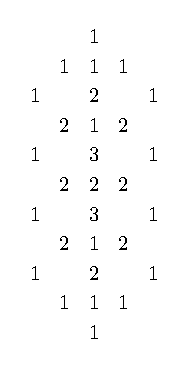
\includegraphics[width=1.7cm]{figures/affine_paving/E6.pdf}
			\vspace{2.9cm}
			\subcaption{$E_6$}
			}
			\parbox[t]{.15\textwidth}{\centering
			\vspace{0cm}
			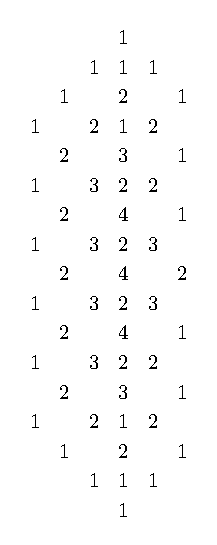
\includegraphics[width=1.7cm]{figures/affine_paving/E7.pdf}
			\vspace{1.95cm}
			\subcaption{$E_7$}
			}
			\parbox[t]{.15\textwidth}{\centering
			\vspace{0cm}
			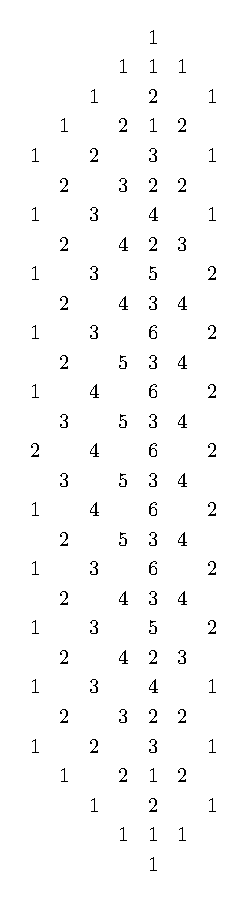
\includegraphics[width=1.7cm]{figures/affine_paving/E8.pdf}
			\subcaption{$E_8$}
			}
		\caption[The quantity $\orde$ for indecomposable representations in type $E$ ]{The quantity $\orde$ for indecomposable representations \\\centering in type $E$ arranged in the Auslander--Reiten quiver \footnotemark}
		\label{fig:startingfunction}
	\end{figure}
\footnotetext{Some representations $M$ are hidden when $\orde(M)=0$. In \cite{bongartz1984critical} the Figure \ref{fig:startingfunction} is called the starting functions\index{starting function|see{order of representation}}.}

For an \textbf{indecomposable} quiver representation $M \in \rep(Q)$, we define the order of $M$\index{order of representation} by
$$\ord(M):= \max_{i \in v(Q)} \dim_{\mathbb{C}} M_i.$$
When the quiver $Q$ is of type $E$, we denote by $e \in v(Q)$ the unique vertex which is connected to three other vertices, and the number 
$$\orde(M):=\dim_\mathbb{C} M_e=[P(e),M]$$
is equal to $\ord(M)$ unless $\orde(M)=0$.

The next lemma shows the affine paving property for representations of small order.

\begin{lemma}[{Follows \cite[Lemma 2.22]{maksimau2019flag}}]\label{lem:smallvecdim}
	Suppose that the underlying graph of $Q$ is a tree. For an indecomposable representation $M \in \rep(Q)$ with $\ord(M) \leqslant 2$, the variety $\Gr_{\ftdimvec{f}}(\Phi(M))$ is either empty or a direct product of some copies of $\mathbb{P}^1$. Especially, the partial flag variety $ \Gr_{\ftdimvec{f}}(\Phi(M))$ has an affine paving.
\end{lemma}
\begin{proof}\belowdisplayskip=-12pt
	For every $i \in v(Q)$, $\dim_\mathbb{C} M_i\leqslant 2$. Since $Q$ is a tree and $M$ is indecomposable, for every $b\in a(Q)$ satisfying $\dim_\mathbb{C} M_{s(b)}= \dim_\mathbb{C} M_{t(b)}=2$, the map $M_{s(b)} \longrightarrow M_{t(b)}$ is an isomorphism. Therefore, when $\Gr_{\ftdimvec{f}}(\Phi(M)) \neq \varnothing$,\footnote{This condition imposes very strong restrictions on $\ftdimvec{f}$.} we get the natural embedding
	$$\Gr_{\ftdimvec{f}}(\Phi(M)) \longrightarrow \prod_{\substack{i \in v(Q) \;s.t.\\ \dim_\mathbb{C} M_i=2 \\ \ftdimvec{f}_{(i,r)}=1 \text{ for some }r}} \mathbb{P}^1,$$\\[0.3cm]
	and the information of non-vertical arrows in the extended quiver (see Example \ref{eg:ext_quiver}) just reduce the number of $\mathbb{P}^1$. Precisely, one need to carefully discuss three cases of $M_i \longrightarrow M_j$:
		% https://q.uiver.app/?q=WzAsNyxbMCwwLCJLIl0sWzMsMCwiSyJdLFsxLDAsIkteMiJdLFsyLDAsIkteMiJdLFs1LDAsIkteMiJdLFs2LDAsIkteMi4iXSxbNCwwLCJcXHRleHR7YW5kfSJdLFs0LDUsIlxcY29uZyJdLFszLDEsIiIsMCx7InN0eWxlIjp7ImhlYWQiOnsibmFtZSI6ImVwaSJ9fX1dLFswLDIsIiIsMCx7InN0eWxlIjp7InRhaWwiOnsibmFtZSI6Imhvb2siLCJzaWRlIjoidG9wIn19fV1d
		\[\begin{tikzcd}
			K & {K^2} & {K^2} & K &[-0.5cm] {\text{and}} &[-0.5cm] {K^2} & {K^2.}
			\arrow["\cong", from=1-6, to=1-7]
			\arrow[two heads, from=1-3, to=1-4]
			\arrow[hook, from=1-1, to=1-2]
		\end{tikzcd}\]
\end{proof}

Now we've nearly prepared every step of the proof of Theorem \ref{thm:Dynkincase}. By following the process in Figure \ref{fig:flowchart}, we now prove Theorem \ref{thm:Dynkincase} assuming Claim \ref{claim:bigorder}. We will prove Claim \ref{claim:bigorder} in Section \ref{appendix:proofcomplement}.

\begin{figure}[ht]
    \centering
    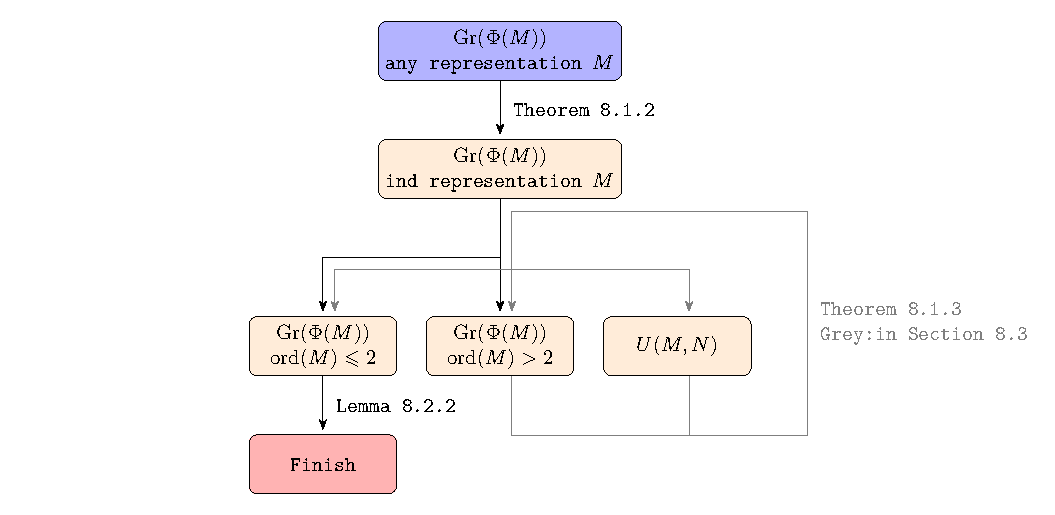
\includegraphics[scale=0.7]{figures/affine_paving/flowchart.pdf}
    \caption[The proof of affine paving in Dynkin case]{The process of induction}
    \vspace{2mm}
    \label{fig:flowchart}
\end{figure}

\begin{claim}\label{claim:bigorder}
Suppose $Q$ is of Dynkin type. For any indecomposable representation $M \in \rep(Q)$ with $\ord(M)>2$, the (strict) partial flag variety $\Gr(\Phi(M))$ has an affine paving.
\end{claim}

\begin{proof}[{Proof of Theorem \ref{thm:Dynkincase}}]
First of all, for any indecomposable representation $M \in \rep(Q)$ we obtain an affine paving. This follows from Claim \ref{claim:bigorder} when $\ord(M)>2$, and follows from Lemma \ref{lem:smallvecdim} when $\ord(M)\leqslant 2$.

The general case follows by induction on the dimension vector. The indecomposable representations $\{N_i\}_{i \in v(Q)}$ of quiver $Q$ can be ordered such that $[N_i,N_j]=0$ for all $i>j$. Therefore, every non-indecomposable representation $M$ can be decomposed as the direct sum of two nonzero representations $M_1, M_2$ satisfying $[M_2,M_1]^1=0$.
By applying Theorem \ref{thm:main1} to the short exact sequence 
$$0 \longrightarrow M_1 \longrightarrow M \longrightarrow M_2 \longrightarrow 0,$$
we get an affine paving from the affine pavings of $M_1$ and $M_2$, see Remark \ref{rem:topo}.
\end{proof}
\begin{remark}\label{rem:smallorder}
By the same technique one can show that, for Dynkin quiver $Q$ and any representation $M$ with $\displaystyle\max_{i \in v(Q)} \dim_\mathbb{C} M_i \leqslant 2$, the variety $\Gr_{\ftdimvec{f}}(\Phi(M))$ has an affine paving. This result does not depend on Claim \ref{claim:bigorder}.
\end{remark}






%%%%%%%%%%%%%%%%%%%%%%%%%%%%%%%%%%%%%%%%%%%%%
%%%%%%%%%%%%%%%%%%%%%%%%%%%%%%%%%%%%%%%%%%%
\section{Proof of Claim \otherrobustref}\label{appendix:proofcomplement}

The task of this section is to prove Claim \ref{claim:bigorder}. When the quiver $Q$ is of type $A$ or $D$, Claim \ref{claim:bigorder} is trivially true since no indecomposable representation can have order bigger than two. So we only concentrate on type $E$.

The idea of the proof is as follows. For any indecomposable representation $Y$ with $\ord(Y)>2$, we put $Y$ into a short exact sequence 
$$\eta:0\longrightarrow X \longrightarrow Y \longrightarrow S \longrightarrow 0$$
fulfilling the assumptions of Theorem \ref{thm:main2}, and then $\Gr(\Phi(Y))$ has an affine paving if $\Img \Psi$ has. If additionally the map $X \hookrightarrow Y$ is a minimal sectional mono, then $\Img \Psi_{\ftdimvec{f},\ftdimvec{g}}$ can be written as the product space, which makes $\Img \Psi$ easier to understand.



\begin{figure}[ht]
\centering
    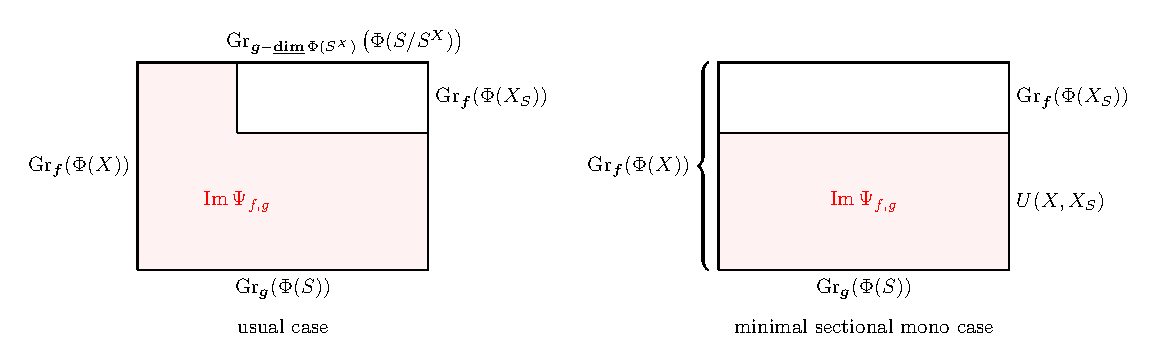
\includegraphics[scale=0.7]{figures/affine_paving/preferredimage.pdf}
\end{figure}

The next two lemmas tell us the existence of the desired short exact sequence.
\begin{lemma}\label{lem:msm&order}
	For every indecomposable representation $Y$ of type $E$ with $\ord(Y)>2$, there is a minimal sectional mono $f:X \longrightarrow Y$.
\end{lemma}
\begin{proof}
	Just observe the Auslander--Reiten quiver. The chosen minimal sectional monos are represented in Figure \ref{fig:minisecmono}. Notice that for the most time $\orde(-)$ is enough to guarantee the map to be a mono.
\end{proof}
		\begin{figure}[ht]
		\centering
			\vspace{0cm}
			\parbox[t]{.15\textwidth}{\centering
			\vspace{0cm}
			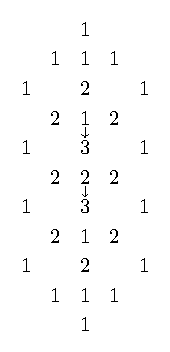
\includegraphics[width=1.7cm]{figures/affine_paving/E6easy.pdf}
			\vspace{4.14cm}
			\subcaption{$E_6$}
			}
			\parbox[t]{.20\textwidth}{\centering
			\vspace{0cm}
			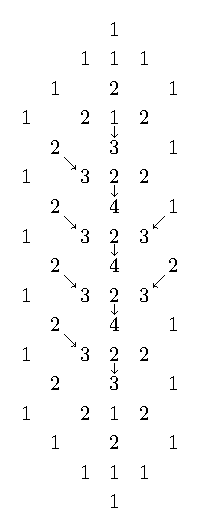
\includegraphics[width=1.7cm]{figures/affine_paving/E7easy.pdf}
			\vspace{3.17cm}
			\subcaption{$E_7$}
			}
			\parbox[t]{.20\textwidth}{\centering
			\vspace{0cm}
			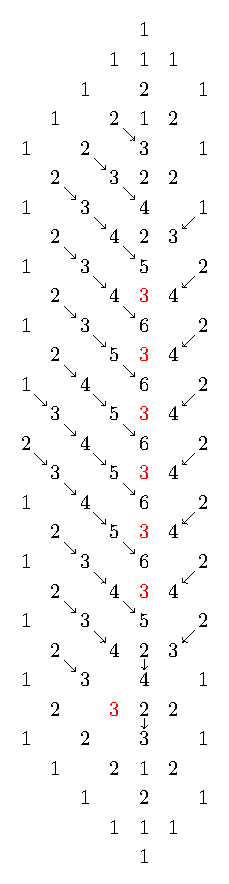
\includegraphics[width=2cm]{figures/affine_paving/E8easy.pdf}
			\subcaption{$E_8$ easy situation}
			}
			\parbox[t]{.2\textwidth}{\centering
			\vspace{0cm}
			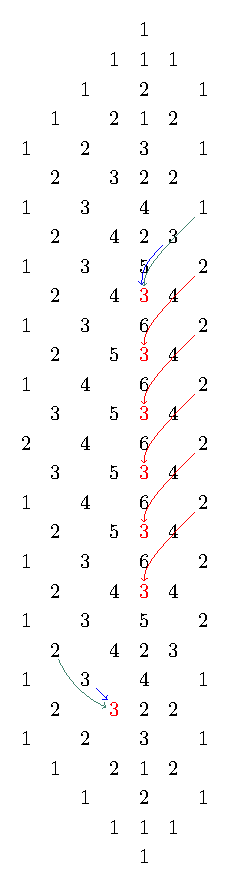
\includegraphics[width=2cm]{figures/affine_paving/E8hard.pdf}
			\subcaption{$E_8$ some exceptions}
			}
			\caption[The chosen minimal sectional monos for complicated indecomposable representations]{Minimal sectional monos}
			\label{fig:minisecmono}
		\end{figure}
\begin{remark}
	The condition $\ord(Y)>2$ in the lemma can not be removed.
\end{remark}
\begin{lemma}\label{lem:value}
Let $X \hookrightarrow Y$ be a minimal sectional mono, and $S:=Y/X$ be the quotient. Then we have the short exact sequence 
$$\eta: 0 \longrightarrow X \longrightarrow Y \longrightarrow S \longrightarrow 0$$
and the dimensions of extension groups among $X,Y,S$ are as shown in the Table \ref{table:dim}.
\renewcommand{\arraystretch}{1.1}
%https://tex.stackexchange.com/questions/552563/centering-on-the-last-column-messes-table-up
\begin{table}
\centering
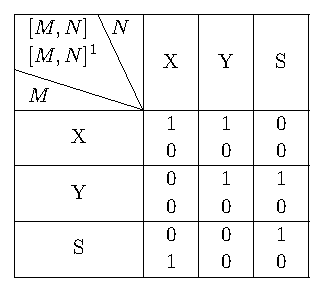
\includegraphics[width=5cm]{figures/affine_paving/dimension_Ext.pdf}
\vspace{1mm}
\caption[Dimension of Extension groups]{}
\label{table:dim}
\end{table}

In particular, $S$ is indecomposable and rigid; $[S,X]^1 =1$, so $X_S$ and $S^X$ are well-defined.
\end{lemma}
\begin{proof}
Since every indecomposable representation of Dynkin quiver is a brick, we get $[X,X]=[Y,Y]=1$ and $[X,X]^1=[Y,Y]^1=0$. By the definition of minimal sectional mono, we get
$[X,Y]=1, [Y,X]=0$ and $[X,Y]^1=[Y,X]^1=0$. By applying the functors $[Y,-],[-,S],[X,-],[-,X],[-Y]$ to the short exact sequence $\eta$ we get the results. 
\end{proof}
In the following two lemmas we will describe the representations $S^X$ and $X_S$ more clearly.

%%%%%%%%%%%%%%%%%%%%%%%%%%%%%%%%???Here we begin to correct mistakes
\begin{lemma} Take the same notations as in Lemma \ref{lem:value}. Then $S^X=S$.
\end{lemma}
\begin{proof}
	Let $\iota:N \longrightarrow S$ be a proper non-zero subrepresentation of $S$, we need to prove that $\iota^* \eta: 0\longrightarrow X \longrightarrow Y' \longrightarrow N \longrightarrow 0$ splits.
	

\[
\begin{tikzcd}
\iota^*\eta: & 0 \arrow[r] & X \arrow[r, hook'] \arrow[d, equal] & Y' \arrow[r] \arrow[d, "h", hook'] & N \arrow[r] \arrow[d, "\iota", hook'] & 0 \\
\eta:        & 0 \arrow[r] & X \arrow[r]                                       & Y \arrow[r]                           & S \arrow[r]                           & 0
\end{tikzcd}
\]
	
	We decompose $Y'=\oplus_i Y_i'$ as the direct sum of indecomposable representations. Since the map $X\longrightarrow Y$ is the minimal sectional mono, we get $Y_i'=X$ or $Y_i'=Y$ or $X\stackrel{0}{\longrightarrow} Y_i'$ for each $i$.
	If there exists $i$ such that $Y_i'=X$, then $\iota^* \eta $ splits; if there exists $i$ such that $Y_i'=Y$, then $h$ is isomorphism, we get $\iota$ is isomorphism; if for every $i$ the map $X \longrightarrow Y_i'$ is $0$, then the map $X \longrightarrow Y'$ is $0$, we also get the contradiction.
\end{proof}

\begin{lemma}[{Follows \cite[Lemma 36]{irelli2019cell}, with the same proof}]\label{lem:descriptionofX_S}
	Let $E \longrightarrow X$ be the minimal right almost split morphism ending in $X$, then we can decompose $E$ as $E=E' \oplus \tau X_1$.\footnote{$X_1$ is defined in Definition \ref{def:sec_morphism}, where we take $M=X$ and $N=Y$.} When $Y$ is not projective, $X_S$ is isomorphic to $\ker (E \longrightarrow \tau Y) \cong E' \oplus \ker (\tau X_1 \longrightarrow \tau Y)$; when $Y$ is projective, $X_S \cong E$.
\end{lemma}
\begin{corollary}
	When $X \longrightarrow Y$ is irreducible monomorphism, the representation $X_S$ is either $0$ or an indecomposable representation with property that $X_S \longrightarrow X$ is also an irreducible monomorphism.
\end{corollary}
\begin{remark}
	We can not copy everything in \cite[Lemma 56]{irelli2019cell}, sometimes it would happen that $X_S=F \oplus T$ with $F$ and $T$ indecomposable, $F \hookrightarrow X$ is irreducible but $T \longrightarrow X/F$ is not a sectional mono. Even when $X_S$ is indecomposable, the map $X_S \longrightarrow X$ can be not a sectional mono.
	
	For example, take the quiver of type $E_7$: 
	\[
	\begin{tikzcd}[row sep=3mm, column sep=5mm]
	                &                 &                 & \bullet \arrow[d] &                 &                 \\
	\bullet \arrow[r] & \bullet \arrow[r] & \bullet \arrow[r] & \bullet           & \bullet \arrow[l] & \bullet \arrow[l]
	\end{tikzcd}
	\]
	 take $Y=\representation{111111}{0}$, $X=\representation{111110}{0}$, then $X_S=\representation{111100}{0}$, the map $X_S \longrightarrow X$ is not a sectional mono.
\end{remark}

Luckily, we can avoid this bad situation by carefully choosing the minimal sectional mono $X \longrightarrow Y$. The minimal sectional monos I chose are presented in Figure \ref{fig:minisecmono}.  We will write down the induction process in detail for some examples.

For convenience, we simplify the notations: write $\Gr_{\ftdimvec{f}}(\Phi(M))$ as $\Gr(M)$, $\Gr_{\ftdimvec{f}}(\Phi(M)) \setminus \Gr_{\ftdimvec{f}}(\Phi(N))$ as $U(M,N)$, where we omit subscripts which indicate the dimension vectors.

\begin{lemma}[{Follows \cite[Theorem 59]{irelli2019cell}}]\label{lem:worst_case}
Let $f:X \hookrightarrow Y$ be a minimal sectional mono and $S:=Y/X$ be the quotient. When $X_S=F \oplus T$ with $F$ and $T$ nonzero indecomposable, $F\hookrightarrow X$ irreducible and $T \hookrightarrow X/F$ sectional mono, we have
$$U(X,X_S)\longrightarrow \Gr(F) \shorttimes U(X/F,T) \oder U(F,F_{X/F})$$
as a Zarisky-locally trivial affine bundle.
\end{lemma}

%https://tex.stackexchange.com/questions/66152/pushing-qed-to-the-right-within-a-displayed-formula
\begin{proof}
We have two short exact sequence satisfying the conditions in \ref{thm:main2}:
\begin{center}
% https://tikzcd.yichuanshen.de/#N4Igdg9gJgpgziAXAbVABwnAlgFyxMJZARgBoAGAXVJADcBDAGwFcYkRyQBfU9TXfIRQAmCtTpNW7AGLdeIDNjwEiAZjE0GLNohAANOXyWCiAFg0Tt7PQHpZPIwJUoArBa1TdnBwv7KhJKTE4h46HIa+xs7IbsGakmHe8opOAaJxlp4gACoRKf5qQSEJ1nZ5fiYo5hmhpXoA+gDK5VEB5O4lugA6XTA49Lo++ZXI7TWdID0AHliD4jBQAObwRKAAZgBOEAC2SG4gOBBIAOw+mzsnNIdIABxnW7uIN1dHiACc8VbdXWhYAOQRc6PD4HV4ANnuF0Q6lBSFMkMeolh0M+WR6v0BDyQZGRwgRSHayOIXEoXCAA
\begin{tikzcd}[row sep=0mm]
\eta: & 0 \arrow[r] & F \arrow[r] & X \arrow[r, "\pi"]    & X/F \arrow[r]   & 0 \\
\xi:  & 0 \arrow[r] & T \arrow[r] & X/F \arrow[r, "\pi'"] & X/X_S \arrow[r] & 0.
\end{tikzcd}
\end{center}
Let $N \in \Gr(X)$ be a subrepresentation, it is obvious that $N \in \Gr(X_S) \iff \pi'\circ \pi(N)=0$, so 
  \begin{equation*}
  \begin{aligned}
  N\in U(X,X_S) & \iff \pi'\circ \pi(N) \neq 0\\
  & \iff \pi(N) \notin \Gr(T)\\
  & \iff \pi(N) \in U(X/F,T)\\
  & \iff \Psi_{\eta}(N) \in \Gr(F) \times U(X/F,T).
  \end{aligned}
  \end{equation*}
Thus the Zarisky-locally trivial affine bundle map
$$U(X,F) \longrightarrow \Gr(F) \shorttimes \Gr(X/F)$$
restricted to the Zarisky-locally trivial affine bundle map

\vspace{\abovedisplayskip}
\hfill $\displaystyle U(X,X_S) \longrightarrow \Gr(F) \times U(X/F,T).$ \qedhere
\end{proof}

We conclude Theorem \ref{thm:main2}, Lemma \ref{lemma:second_description_XS}, \ref{lem:value}, \ref{lem:descriptionofX_S}, \ref{lem:worst_case} in the following proposition.

\begin{proposition}\label{prop:conclusion_for_combinatorics}
Let $f:X \hookrightarrow Y$ be a minimal sectional mono and $S:=Y/X$ be the quotient. One get Zariski-locally affine maps
\begin{equation*}
\begin{aligned}
\Gr(Y) &\longrightarrow \Gr(X) \shorttimes \Gr(S) \oder U(X,X_S), \\
U(Y,X) &\longrightarrow \Gr(X) \shorttimes \Gr(S) \oder U(X,X_S), \\
\end{aligned}
\end{equation*}
where
\begin{equation*}
\begin{aligned}
  X_S:=\;& \max \left\{ M \subseteq X \,\middle|\; [S,X/M ]^1=1 \right\} \\ 
  =\;& \ker (X \longrightarrow \tau S) \\ 
  =\;& \begin{cases}
  E' \oplus \ker (\tau X_1 \longrightarrow \tau Y) & Y \text{ not projective, }\\
  E & Y \text{ projective. }
  \end{cases} \\ 
\end{aligned}
\end{equation*}
Moreover, when $X_S=F \oplus T$ with $F$ and $T$ nonzero indecomposable, $F\hookrightarrow X$ irreducible and $T \hookrightarrow X/F$ sectional mono, one get a Zariski-locally affine map
$$U(X,X_S)\longrightarrow \Gr(F) \shorttimes U(X/F,T) \oder U(F,F_{X/F}).$$
\end{proposition}

With Proposition \ref{prop:conclusion_for_combinatorics} in hand, we prove Claim \ref{claim:bigorder} by cases, which turns out to be a pure combinatorical problem. 

\begin{proof}[{Proof of Claim \ref{claim:bigorder}}]
When the minimal sectional mono $X \longrightarrow Y$ is irreducible, we use Theorem \ref{thm:main2} to get morphism
$$\Gr(Y) \longrightarrow \Gr(X) \shorttimes \Gr(S) \oder U(X,X_S).$$ 
By observation of  Figure \ref{fig:minisecmono}, $\orde(S)=\orde(Y)-\orde(X)$ is smaller or equal to $2$, so by Lemma \ref{lem:smallvecdim} $\Gr(S)$ has the affine paving property. Let $Y':=X$, $X':=X_S$, $S':=Y'/X'$, we again use Theorem \ref{thm:main2} to get Zariski-locally affine maps
\begin{equation*}
\begin{aligned}
\Gr(X) &\longrightarrow \Gr(X') \shorttimes \Gr(S') \oder U(X',X'_{S'}) \\
U(X,X_S)&\longrightarrow \Gr(X') \shorttimes \Gr(S') \oder U(X',X'_{S'}).
\end{aligned}
\end{equation*}
Luckily $\orde(S')$ is still smaller or equal to $2$. We can continue this process until the order of representations are small enough.

The exceptional cases are similar, but the discussion is a bit more complicated. Let us look at some examples. 
\captionsetup[subfigure]{labelfont=rm}
\captionsetup[subfigure]{labelformat=parens}
%https://tex.stackexchange.com/questions/233481/subcaption-defaulting-to-capital-letter-labels

		\begin{figure}[ht]
		\centering
			\vspace{0cm}
			\parbox[b]{.23\textwidth}{\centering
			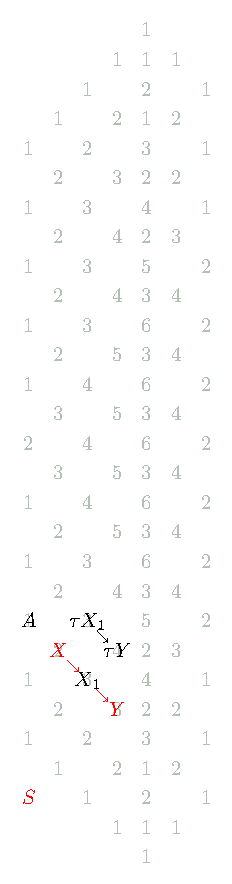
\includegraphics[width=32mm]{figures/affine_paving/E8graypic1.pdf}
			\subcaption{}
			}
			\parbox[b]{.23\textwidth}{\centering
			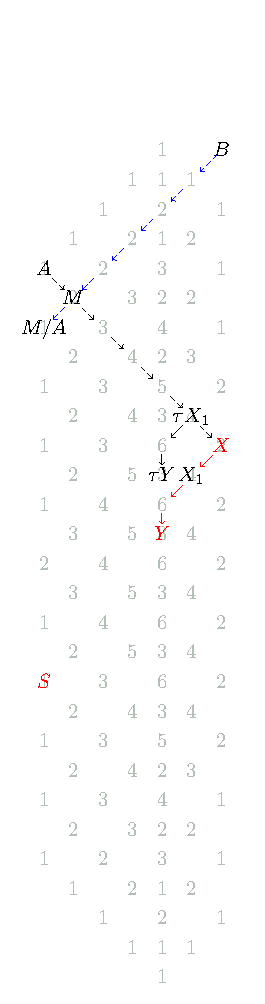
\includegraphics[width=32mm]{figures/affine_paving/E8graypic2.pdf}
			\subcaption{}
			}
			\parbox[b]{.23\textwidth}{\centering
			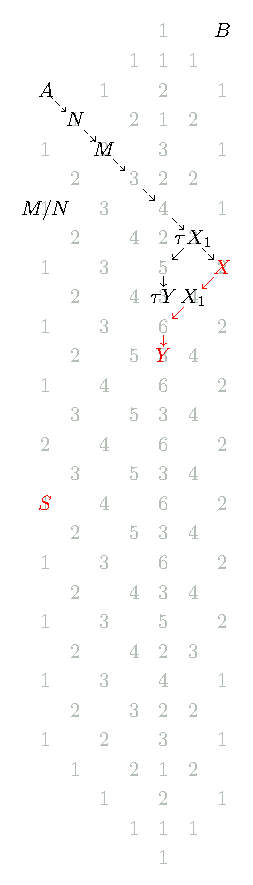
\includegraphics[width=32mm]{figures/affine_paving/E8graypic3.pdf}
			\subcaption{}
			}
			\parbox[b]{.23\textwidth}{\centering
			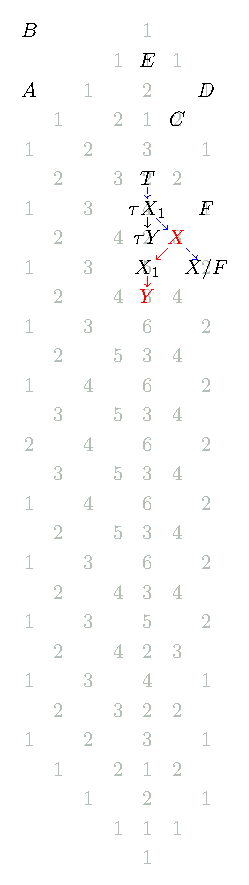
\includegraphics[width=32mm]{figures/affine_paving/E8graypic4.pdf}
			\vspace{-0.75mm}
			\subcaption{}
			}
			\caption[A detailed discussion of the exceptional cases]{Special cases}
			\label{fig:specialcases}
			\vspace{0.2cm}
		\end{figure}

\begin{eg}
In the case of Figure \ref{fig:specialcases}(a), if $X_1 \longrightarrow Y$ is injective, then we obtain some Zariski-locally affine maps
\begin{equation*}
\begin{aligned}
\Gr(Y) &\longrightarrow \Gr(X_1) \shorttimes \Gr(Y/X_1) &&\oder U(X_1,X)\\
\Gr(X_1) &\longrightarrow \Gr(X) \shorttimes \Gr(X_1/X) &&\oder U(X,A)\\
U(X_1,X) &\longrightarrow \Gr(X) \shorttimes \Gr(X_1/X) &&\oder U(X,A)\\
U(X,A) &\longrightarrow \Gr(A) \shorttimes \Gr(X/A) &&\oder U(A,-).\footnotemark \\
\end{aligned}
\end{equation*}
\footnotetext{$\Gr(A)$ is empty or a singleton, so is $U(A,-)$, no matter what representation is in the dash mark.}
When $X_1 \longrightarrow Y$ is not injective, we get
\begin{equation*}
\begin{aligned}
\Gr(Y) &\longrightarrow \Gr(X) \shorttimes \Gr(X/Y)\hspace{3mm} &&\oder U(X,A)\\
U(X,A) &\longrightarrow \Gr(A) \shorttimes \Gr(X/A) &&\oder U(A,-).\\
\end{aligned}
\end{equation*}
These maps give the variety $\Gr(Y)$ an affine paving from bottom to top.
\end{eg}
\begin{eg}
In Figure \ref{fig:specialcases}(b), we would like to prove that  $\Gr(Y)$ has the affine paving property. We have
$$\Gr(Y) \longrightarrow \Gr(X) \shorttimes \Gr(Y/X) \oder U(X,A).$$
When the map $M \longrightarrow X$ is not monomorphism, we get
$$U(X,A) \longrightarrow \Gr(A) \shorttimes \Gr(X/A) \oder U(A,-);$$
when the map $M \longrightarrow X$ is monomorphism, we get
%tex.stackexchange.com/questions/453057/alignment-in-cases-with-text-outside-the-cases
%https://tex.stackexchange.com/questions/483234/align-text-in-a-cases-environment-with-text-outside
\begin{equation*}
\begin{aligned}
&U(X,A)=U(X,M) \bigsqcup U(M,A)\hspace{-30mm}&&\\
U(X,M) &\longrightarrow \Gr(M) \shorttimes \Gr(X/M) && \oder U(M,A \oplus B)\\
U(M,A) &\longrightarrow \Gr(A) \shorttimes \Gr(M/A)&& \oder U(A,-)\\
U(M,A \oplus B)  &\longrightarrow \begin{cases}
\Gr(A) \shorttimes \Gr(M/A)\\
\Gr(A) \shorttimes U(M/A,B)\\
\end{cases} \hspace{-5mm}&& \begin{aligned}
\oder U(A,-), &\qquad B=0,\\
\oder U(A,-), &\qquad B\neq 0.
\end{aligned}\\
\end{aligned}
\end{equation*}

Since the order of $X$, $Y/X$, $A$, $X/A$, $M$, $X/M$, $M/A$ are smaller or equal to $2$ as well as $\ord(A)=\ord(M/A)=1$, the induction process stops, we get an affine paving of $\Gr(Y)$.
\end{eg}
\begin{eg}
In the case of Figure \ref{fig:specialcases}(c), we have 
$$\Gr(Y) \longrightarrow \Gr(X) \shorttimes \Gr(Y/X) \oder U(X,A).$$
If $A=0$, we're done; if not, we decompose $A \longrightarrow Y$ as compositions of minimal sectional monos:\\
Case 1: $M\longrightarrow X$ is not injective, then
 \begin{equation*}
 \begin{aligned}
 &U(X,A)=U(X,N) \bigsqcup U(N,A)\\
 U(X,N) &\longrightarrow \Gr(N) \shorttimes \Gr(X/N) \oder U(N,-)\\
 \end{aligned}
 \end{equation*}
Case 2: $M\longrightarrow X$ is injective, then
  \begin{equation*}
  \begin{aligned}  
  U(X,A)&=U(X,M) \bigsqcup U(M,N) \bigsqcup U(N,A)\hspace{-20mm}&&\\
  U(X,M) &\longrightarrow \Gr(M) \shorttimes \Gr(X/M) &&\hspace{-3mm} \oder U(M,N \oplus T)\\
  U(M,N) &\longrightarrow \Gr(N) \shorttimes \Gr(M/N)&&\hspace{-3mm} \oder U(N,-),\\
  \end{aligned}
  \end{equation*}
  Since $M \longrightarrow X$ is injective, we get $B=0$, thus $C=0$ also, and then the sectional map $T \longrightarrow M/N$ is injective. We get 
  $$  U(M,N \oplus T)  \longrightarrow 
    \Gr(N) \shorttimes U(M/N,T)
    \oder U(N,-).$$
  Since $\Gr(X)$, $\Gr(Y/X)$, $\Gr(N)$, $\ldots$ have the property of affine paving, we conclude that $\Gr(Y)$ also has the property of affine paving.
\end{eg}
\begin{eg}
Finally we begin to tackle the most difficult case(Figure \ref{fig:specialcases}(d)). When $X \longrightarrow Y$ is not injective, we get
$$\Gr(Y) \longrightarrow \Gr(F) \shorttimes \Gr(Y/F) \oder U(F,-),\hspace{8mm}$$
and then we get the result.

When $X \longrightarrow Y$ is injective (i.e., $A=0$), we have
$$\Gr(Y) \longrightarrow \Gr(X) \shorttimes \Gr(Y/X) \oder U(X,F \oplus T).$$
Notice that

$$A=0 \hspace{4mm}\Longrightarrow \begin{cases}
\hspace{4mm}B=0  \hspace{4mm}\Longleftrightarrow\hspace{4mm} T  \longrightarrow X/F \text{ is injective}\\
\hspace{4mm}C=0  \hspace{4mm}\Longleftrightarrow\hspace{4mm} G  \longrightarrow T \text{ is injective}\\
\hspace{4mm}D=0  \hspace{4mm}\Longleftrightarrow \hspace{4mm}I  \longrightarrow G/H \text{ is injective}\\
\end{cases}$$
We get 
\begin{equation*}
\begin{aligned}
U(X,F \oplus T) &\longrightarrow \Gr(F) \shorttimes U(X/F,T) &&\oder U(F,-)\\
U(X/F,T) &\longrightarrow \Gr(T) \shorttimes \Gr(X/X_S) &&\oder U(T,G)\\
U(T,G) &\longrightarrow \Gr(G) \shorttimes \Gr(T/G) &&\oder U(G,H \oplus I)\\
U(G,H \oplus I) &\longrightarrow \Gr(H) \shorttimes U(G/H,I) &&\oder U(H,-). \\
\end{aligned}
\end{equation*}
We conclude that $\Gr(Y)$ has the affine paving property.\qedhere
\end{eg}
\end{proof}

%%%%%%%%%%%%%%%%%%%%%%%%%%%%%%%%%%%%%%%%%%%%%%%%%%%%%%%%%%%%%%%%%%%%%%%%%%%%%%%%%%%%%%%%%%%%%%%
\section{Application: affine case}\label{sec:affine}
This section tries to explain the difficulty of the Conjecture \ref{conj:affinecase}.

\begin{conj}\label{conj:affinecase}
For any affine quiver $Q$ and any indecomposable representation $M \in \rep(Q)$, the (strict) partial flag variety $\Flag{}(M)\cong\Gr(\Phi(M))$ has an affine paving.
\end{conj}

Actually, if readers follow the proof in \cite[Section 6]{irelli2019cell}, and change everything from $\Gr(-)$ to $\Gr(\Phi(-))$, then there is no difference except the Proposition 48, in which the authors proved the affine paving properties of quasi-simple regular representations. So we reduced the question to the case of quasi-simple regular representation. Combined with Lemma \ref{lem:affineADcase}, we've proved the affine paving properties for $\tilde{A},\tilde{D}$ cases.

\begin{lemma}\label{lem:affineADcase}
	Assume that $Q$ is an affine quiver of type $A$ or $D$, $M \in \rep(Q)$ is the \textbf{regular quasi-simple} representation\index{quasi-simple representation}, then the Grassmannian $\Gr(\Phi(M))$ has an affine paving.
\end{lemma}
\begin{proof}
The concept ``quasi-simple'' is defined in \cite[Definition 15]{irelli2019cell}; the concepts ``preprojective'',``preinjective'' and ``regular'' are defined in \cite[2.1.1]{irelli2019cell}. It's shown in \cite[Section 9, Lemma 3]{crawley1992lectures} that the regular quasi-simple representation $M$ have dimension vector smaller or equal to the minimal positive imaginary root, thus $\orde(M) \leqslant 2$ for the quiver of type $\tilde{D}$ and $\orde(M) \leqslant 1$ for the quiver of type $\tilde{A}$.
\end{proof}
%We use rep 2 Cor 18.8.

\begin{theorem}\label{thm:affinecase}\
\begingroup
\upshape
\begin{enumerate}[(1)]
\item Assume that $Q$ is an affine quiver of type $A$ or $D$, then for any indecomposable representation $M$, the Grassmannian $\Gr(\Phi(M))$ has an affine paving;
\item Assume that $Q$ is an affine quiver of type $E$, and $\Gr(\Phi(N))$ has an affine paving for any regular quasi-simple representation $N \in \rep(Q)$. The Grassmannian $\Gr(\Phi(M))$ then has an affine paving for any indecomposable representation $M$.
\end{enumerate}
\endgroup
\end{theorem}

For a regular quasi-simple representation $Y$ of type $\tilde{E}$, it's possible that there's no short exact sequence
$$\eta:0\longrightarrow X \longrightarrow Y \longrightarrow S \longrightarrow 0$$
such that $[S,X]^1 \leqslant 1$. Then we can no longer use Theorem \ref{thm:main1} or \ref{thm:main2}. Hence, the new methods are needed for this case.
%\appendix
%\setcounter{secnumdepth}{0}
%\section{Appendix}





%https://tex.stackexchange.com/questions/14510/how-to-show-listoffigures-and-listoftables-on-one-page-and-in-the-toc
%https://tex.stackexchange.com/questions/30747/remove-newpage-after-tableofcontents-listoffigures-etc-in-book-class


\begingroup
\let\cleardoublepage\relax
%\let\clearpage\relax
\addcontentsline{toc}{chapter}{List of Tables}
\listoftables
\addcontentsline{toc}{chapter}{List of Figures}
\listoffigures
\endgroup

\addcontentsline{toc}{chapter}{Bibliography}
\bibliographystyle{plain}
\bibliography{reference}
\end{document}




